\documentclass[11pt]{article}
\usepackage[paperwidth=8.5in, paperheight=13in, top=0.75in, bottom=0.75in, right=0.75in, left=1.25in]{geometry}
\usepackage[utf8]{inputenc}
\usepackage{amsmath, amssymb, amsfonts, fancybox, xcolor, mathrsfs, verbatim, xspace, tikz, setspace, graphicx, multicol, ifthen, calc, fancyhdr, enumitem, textcomp, pgfplots, mathtools, bm, esvect, harpoon, array, circuitikz,float, xcolor}
\usepackage{enumitem}
\usetikzlibrary{patterns}
\usetikzlibrary{arrows.meta,bending}


\begin{document}
  \thispagestyle{empty} 

  \begin{figure}
    \centering
    \includegraphics[width=0.2\textwidth]{pup logo.jpg}
  \end{figure}

  \begin{center}
    {\Large
    Polytechnic University of the Philippines\\
    College of Engineering\\
    Computer Engineering Department\\
    }
  \end{center}

\vfill

  \begin{center}
    {\Large \textbf{Solved Problems in Feedback and Control Systems}} \\ 
    {\large (Electrical Network Transfer Functions,
Translational Mechanical System Transfer \\Functions,
Rotational Mechanical System Transfer Functions,
Transfer Function \\involving Gears, 
Electromechanical System Transfer Function,
Block Diagram \\Algebra, and Signal Flow Graphs)}
  \end{center}

\vfill

  \begin{center}
    {\large
    Completion requirement for the subject\\
    CMPE 309 - Feedback and Control Systems\\
    }
  \end{center}

\vfill

  \begin{center}
    {\large 
    TUAZON, Ivan Lawrence O. \\
    2022-09851-MN-0\\
    Bachelor of Science in Computer Engineering\\
    }
  \end{center}

\vfill

  \begin{center}
    Engr. John R. Dela Cruz, MSECE, PECE, AAE, 1PHN\\
    Faculty-in-charge
  \end{center}

\vfill

  \begin{center}
    August 2025
  \end{center}



%  Problem 1 - Electrical Network Transfer Functions,

\newpage
  \setcounter{page}{1}  
\noindent\rule{\textwidth}{1pt}
\noindent\textbf{Problem 1} \hfill
\\Find the transfer function, G(s) = VL(s)/V(s) , of the given circuit. Use Mesh Analysis

\begin{figure}[!ht]
\centering
\resizebox{0.5\textwidth}{!}{%
\begin{circuitikz}
\tikzstyle{every node}=[font=\large]
\draw [short] (-2.75,21.75) -- (-0.25,21.75);
\draw (-0.25,21.75) to[L ] (1.75,21.75);
\draw [short] (1.75,21.75) -- (4.25,21.75);
\draw [short] (-2.75,19.25) -- (-2.75,21.75);
\draw (-2.75,19.25) to[R] (0.75,19.25);
\draw [short] (4.25,19.25) -- (4.25,21.75);
\draw (0.75,19.25) to[R] (4.25,19.25);
\draw (0.75,19.25) to[L ] (0.75,15.75);
\draw (4.25,19.25) to[L ] (4.25,15.75);
\draw [short] (-2.75,15.75) -- (4.25,15.75);
\draw (-2.75,19.25) to[american voltage source] (-2.75,15.75);
\node [font=\large] at (0.75,22.5) {1 H};
\node [font=\large] at (0,17.5) {1 H};
\node [font=\large] at (3.5,17.5) {1 H};
\node [font=\large] at (-1,19.75) {1 $\Omega$};
\node [font=\large] at (2.5,19.75) {1 $\Omega$};
\node [font=\large, color={rgb,255:red,46; green,128; blue,163}] at (-3.5,17.5) {v(t)};
\node [font=\large, color={rgb,255:red,46; green,128; blue,163}] at (5.25,17.5) {$v_L(t)$};
\node [font=\large, color={rgb,255:red,46; green,128; blue,163}] at (4.75,18.25) {$+$};
\node [font=\large, color={rgb,255:red,46; green,128; blue,163}] at (4.75,16.75) {$-$};
\end{circuitikz}
}%
\end{figure}

\noindent\rule{\textwidth}{1pt}


\vspace{12pt}

\noindent\textbf{\textit{Given:}}  
\ The electrical circuit converted to the Laplace domain with impedances:
\[
\begin{aligned}
R_1 &= 1\, \Omega, \quad R_2 = 1\, \Omega, \\
L_1 &= 1\, \text{H}, \quad L_2 = 1\, \text{H}, \quad L_3 = 1\, \text{H}
\end{aligned}
\]

\vspace{12pt}

\noindent \textbf{\textit{Required:}}
Find the Transfer Function:
\[
G(s) = \frac{V_L(s)}{V(s)}
\]

\vspace{12pt}

\noindent \textbf{\textit{Solution:}}

\vspace{12pt}

{Let the mesh currents be:}
\[
I_1, \quad I_2, \quad I_3
\]

\vspace{12pt}

{Writing the Mesh Equations}
\[
(s + 1) I_1(s) - s I_2(s) - I_3(s) = V(s)
\]
\[
- s I_1(s) + (2s + 1) I_2(s) - I_3(s) = 0
\]
\[
- I_1(s) - I_2(s) + (s + 2) I_3(s) = 0
\]

{Matrix Representation}
\[
\begin{bmatrix}
s + 1 & -s & -1 \\
-s & 2s + 1 & -1 \\
-1 & -1 & s + 2
\end{bmatrix}
\begin{bmatrix}
I_1 \\ I_2 \\ I_3
\end{bmatrix}
=
\begin{bmatrix}
V(s) \\ 0 \\ 0
\end{bmatrix}
\]

We seek  \(V_L(s) = s I_2(s)\).

\vspace{1em}

\noindent\textbf{Solving for \(I_2(s)\)}

\vspace{1em}

{Using Cramer's rule:}
\[
I_2(s) = \frac{
\begin{vmatrix}
s + 1 & V(s) & -1 \\
-s & 0 & -1 \\
-1 & 0 & s + 2
\end{vmatrix}
}{
\begin{vmatrix}
s + 1 & -s & -1 \\
-s & 2s + 1 & -1 \\
-1 & -1 & s + 2
\end{vmatrix}
}
\]

Solving the determinants:
\[
I_2(s) = \frac{(s^2 + 2s + 1) V(s)}{s(s^2 + 5s + 2)}
\]

Therefore:
\[
V_L(s) = s I_2(s) = \frac{(s^2 + 2s + 1) V(s)}{s^2 + 5s + 2}
\]

\noindent\textbf{Final Transfer Function}

\[
\boxed{
G(s) = \frac{V_L(s)}{V(s)} = \frac{s^2 + 2s + 1}{s^2 + 5s + 2}
}
\]


% Problem 2  Electrical Network Transfer Functions,

\newpage
% command for new page 
  \setcounter{page}{3}  
\noindent\rule{\textwidth}{1pt}
\noindent\textbf{Problem 2} \hfill 
\\ Find the transfer function, $G(s) = \frac{I_1(s)}{V(s)}$, of the given figure.

\begin{figure}[!ht]
\centering
\resizebox{0.6\textwidth}{!}{%
\begin{circuitikz}
\tikzstyle{every node}=[font=\large]

% unified style + size for current loops (Overleaf-friendly)
\tikzset{
  currloop/.style={
    draw,
    color={rgb,255:red,46; green,128; blue,163},
    line width=0.9pt,
    line cap=round,
    -{Stealth[length=2.6mm,width=1.8mm]} % arrow tip sizing
  }
}
\def\rloop{0.70} % loop radius (small + identical)
\newcommand{\loopat}[2]{%
  \draw[currloop] (#1,#2) ++(120:\rloop)
    arc[start angle=120, delta angle=-300, radius=\rloop];
}

% circuit
\draw (3.25,19.5) to[curved capacitor,l={ \large 1 F}] (5.25,19.5);
\draw (1,17.25) to[R,l={ \large 1 $\Omega$}] (2.75,17.25);
\draw (5.5,17.25) to[L,l={ \large 4 H} ] (7.5,17.25);
\draw (4.25,16.75) to[R,l={ \large 1 $\Omega$}] (4.25,15);
\draw (4.25,14.5) to[L,l={ \large 2 H} ] (4.25,12.75);
\draw (8.5,15.75) to[L,l={ \large 3 H} ] (8.5,14);
\draw (0,16) to[american voltage source] (0,14);
\draw [short] (2.75,17.25) -- (5.5,17.25);
\draw [short] (4.25,16.75) -- (4.25,17.25);
\draw [short] (4.25,14.5) -- (4.25,15);
\draw [short] (7.5,17.25) -- (8.5,17.25);
\draw [short] (8.5,17.25) -- (8.5,15.75);
\draw [short] (0,16) -- (0,17.25);
\draw [short] (0,17.25) -- (1,17.25);
\draw [short] (0,14) -- (0,12.75);
\draw [short] (0,12.75) -- (4.25,12.75);
\draw [short] (4.25,12.75) -- (8.5,12.75);
\draw [short] (8.5,12.75) -- (8.5,14);
\draw [short] (5.25,19.5) -- (8.5,19.5);
\draw [short] (8.5,19.5) -- (8.5,17.25);
\draw [short] (3.25,19.5) -- (0,19.5);
\draw [short] (0,19.5) -- (0,17);

% identical current loops
\loopat{2.05}{15.10}  % i1
\loopat{6.35}{15.10}  % i2
\loopat{4.25}{18.20}  % i3

\node [font=\large] at (-1,15.25) {v(t)};
\node [font=\large] at (2,13.75) {$i_1(t)$};
\node [font=\large] at (5.5,18.5) {$i_3(t)$};
\node [font=\large] at (6.5,13.75) {$i_2(t)$};
\end{circuitikz}
}%
\end{figure}
\noindent\rule{\textwidth}{1pt}

\vspace{12pt}


\noindent
\textbf{\textit{Given:}}  
\ The electrical circuit converted to the Laplace domain with impedances:
\[
\begin{aligned}
R_1 &= 1, \quad R_2 = 1, \quad L_1 = 2\, \text{H}, \quad L_2 = 3\, \text{H}, \quad L_3 = 4\, \text{H} \\
C_1 &= 1\, \text{F} \quad \Rightarrow \quad \frac{1}{s} \text{ impedance}
\end{aligned}
\]
\vspace{12pt}

\noindent
\textbf{\textit{Required:}}
    \ Determine the transfer function:
    \[
    G(s) = \frac{I_1(s)}{V(s)}
    \]
\vspace{12pt}

\noindent \textbf{\textit{Solution:}}

\bigskip

{System of Equations:}
\[
\begin{aligned}
(2s + 2)I_1(s) - (2s + 1)I_2(s) - I_3(s) &= V(s) \\
-(2s + 1)I_1(s) + (9s + 1)I_2(s) - 4s I_3(s) &= 0 \\
- I_1(s) - 4s I_2(s) + \left(4s + 1 + \frac{1}{s}\right)I_3(s) &= 0
\end{aligned}
\]

{Matrix Form:}
\[
\begin{bmatrix}
2s + 2 & -(2s + 1) & -1 \\
-(2s + 1) & 9s + 1 & -4s \\
-1 & -4s & 4s + 1 + \frac{1}{s}
\end{bmatrix}
\begin{bmatrix}
I_1(s) \\ I_2(s) \\ I_3(s)
\end{bmatrix}
=
\begin{bmatrix}
V(s) \\ 0 \\ 0
\end{bmatrix}
\]

{Determinant \(\Delta\):}
\[
\Delta =
\begin{vmatrix}
2s + 2 & -(2s + 1) & -1 \\
-(2s + 1) & 9s + 1 & -4s \\
-1 & -4s & 4s + 1 + \frac{1}{s}
\end{vmatrix}
= \frac{24s^4 + 30s^3 + 17s^2 + 16s + 1}{s}
\]

{Using Cramer's Rule for \(I_1(s)\):}
\[
I_1(s) =
\frac{
\begin{vmatrix}
V(s) & -(2s + 1) & -1 \\
0 & 9s + 1 & -4s \\
0 & -4s & 4s + 1 + \frac{1}{s}
\end{vmatrix}
}
{\Delta}
= \frac{V(s)\left(20s^3 + 13s^2 + 10s + 1\right)}{24s^4 + 30s^3 + 17s^2 + 16s + 1}
\]


{Transfer Function:}

\[
\boxed{
G(s) = \frac{I_1(s)}{V(s)} = \frac{20s^3 + 13s^2 + 10s + 1}{24s^4 + 30s^3 + 17s^2 + 16s + 1}
}
\]

% Problem 3  Electrical Network Transfer Functions,
\newpage
  \setcounter{page}{4}
\noindent\rule{\textwidth}{1pt}
\noindent\textbf{Problem 3} \hfill 
\\ Find the transfer function, $\frac{V_O(s)}{V(s)}$, of the given figure.

\begin{figure}[!ht]
\centering
\resizebox{0.6\textwidth}{!}{%
\begin{circuitikz}
\tikzstyle{every node}=[font=\large]

% identical round current loops
\tikzset{
  currloop/.style={
    draw,
    color={rgb,255:red,46; green,128; blue,163},
    line width=0.9pt,
    line cap=round,
    -{Stealth[length=2.6mm,width=1.8mm]}
  }
}
\def\rloop{0.68} % loop radius (all three use this)
\newcommand{\loopat}[2]{%
  \draw[currloop] (#1,#2) ++(120:\rloop)
    arc[start angle=120, delta angle=-300, radius=\rloop];
}

% --- circuit ---
\draw [short] (-2.5,23.5) -- (0,23.5);
\draw [short] (4,23.5) -- (6.5,23.5);
\draw [short] (-2.5,21) -- (-2.5,23.5);
\draw (-2.5,21) to[R] (2,21);
\draw [short] (6.5,21) -- (6.5,23.5);
\draw (2,21) to[R] (4.5,21);
\draw (2,18.5) to[L ] (2,16.75);
\draw [short] (-2.5,16) -- (6.5,16);
\draw (-2.5,21) to[american voltage source] (-2.5,16);
\node [font=\large] at (2,24.25) {9 F};
\node [font=\large] at (1.25,19.75) {2 $\Omega$};
\node [font=\large] at (5.75,18.5) {8$\Omega$};
\node [font=\large] at (-0.25,21.5) {2 $\Omega$};
\node [font=\large] at (3.25,21.5) {4 $\Omega$};
\node [font=\large, color={rgb,255:red,46; green,128; blue,163}] at (-3.5,18.5) {\textit{v(t)}};
\node [font=\large, color={rgb,255:red,46; green,128; blue,163}] at (7.5,18.5) {$v_o (t)$};
\node [font=\large, color={rgb,255:red,46; green,128; blue,163}] at (7,19.25) {$+$};
\node [font=\large, color={rgb,255:red,46; green,128; blue,163}] at (7,17.75) {$-$};
\draw (0,23.5) to[curved capacitor] (4,23.5);
\draw (4.5,21) to[L ] (6.5,21);
\draw (6.5,21) to[R] (6.5,16);
\draw (2,21) to[R] (2,18.5);
\node [font=\large] at (5.5,21.75) {6 H};
\draw [short] (2,16) -- (2,16.75);
\node [font=\large] at (1.25,17.5) {4 H};
\node [font=\large] at (-0.5,17) {$i_1(t)$};
\node [font=\large] at (4.25,17) {$i_2(t)$};
\node [font=\large] at (2,21.25) {$i_3(t)$};

% --- identical round loops (replace your three Bézier arrows) ---
\loopat{-0.20}{18.40}  % i1 loop (bottom-left)
\loopat{ 4.20}{18.40}  % i2 loop (bottom-right)
\loopat{ 2.00}{22.30}  % i3 loop (top)
% ---------------------------------------------------------------
\end{circuitikz}
}%
\end{figure}


\noindent\rule{\textwidth}{1pt}

\vspace{12pt}


\noindent\textbf{\textit{Given:}}  
\ The electrical circuit converted to the Laplace domain with impedances:
\[
\begin{aligned}
R_1 &= 2\, \Omega, \quad R_2 = 4\, \Omega, \quad R_3 = 2\, \Omega, \quad R_4 = 8\, \Omega \\
L_1 &= 4\, \text{H}, \quad L_2 = 6\, \text{H}, \quad C_1 = 9\, \text{F} \quad \Rightarrow \quad \frac{1}{9s} \text{ impedance}
\end{aligned}
\]

 
\vspace{12pt}

\noindent
\textbf{\textit{Required:}}
    \ Determine the transfer function:
    \[
    \frac{V_O(s)}{V(s)}
    \]

\vspace{12pt}

\noindent \textbf{\textit{Solution:}}

\vspace{12pt}

{System of Equations:}
\[
\begin{aligned}
(4s + 4) I_1(s) - (4s + 2) I_2(s) - 2 I_3(s) &= V(s) \\
-(4s + 2) I_1(s) + (10s + 14) I_2(s) - (6s + 4) I_3(s) &= 0 \\
-2 I_1(s) - (6s + 4) I_2(s) + \left(6s + 6 + \frac{9}{s}\right) I_3(s) &= 0
\end{aligned}
\]

\bigskip

{Matrix Form:}
\[
\begin{bmatrix}
4s + 4 & -(4s + 2) & -2 \\
-(4s + 2) & 10s + 14 & -(6s + 4) \\
-2 & -(6s + 4) & 6s + 6 + \frac{9}{s}
\end{bmatrix}
\begin{bmatrix}
I_1(s) \\ I_2(s) \\ I_3(s)
\end{bmatrix}
=
\begin{bmatrix}
V(s) \\ 0 \\ 0
\end{bmatrix}
\]

\bigskip

{Determinant \( \Delta \):}
\[
\Delta = 
\begin{vmatrix}
4s + 4 & -(4s + 2) & -2 \\
-(4s + 2) & 10s + 14 & -(6s + 4) \\
-2 & -(6s + 4) & 6s + 6 + \frac{9}{s}
\end{vmatrix}
= \frac{4\left(48s^3 + 150s^2 + 220s + 117\right)}{s}
\]

\bigskip

{Using Cramer's Rule for \(I_2(s)\):}
\[
I_2(s) = 
\frac{
\begin{vmatrix}
4s + 4 & V(s) & -2 \\
-(4s + 2) & 0 & -(6s + 4) \\
-2 & 0 & 6s + 6 + \frac{9}{s}
\end{vmatrix}
}
{\Delta}
= \frac{V(s)\left(12s^3 + 24s^2 + 28s + 9\right)}{2 \left(48s^3 + 150s^2 + 220s + 117\right)}
\]

\bigskip

{Output Voltage:}
\[
V_O(s) = 8 I_2(s)
\]
\[
V_O(s) = \frac{4V(s)\left(12s^3 + 24s^2 + 28s + 9\right)}{48s^3 + 150s^2 + 220s + 117}
\]

\bigskip

{Transfer Function:}
\[
\boxed{
\frac{V_O(s)}{V(s)} = \frac{4\left(12s^3 + 24s^2 + 28s + 9\right)}{48s^3 + 150s^2 + 220s + 117}
}
\]

% Problem 4  Electrical Network Transfer Functions,
\newpage
  \setcounter{page}{6}  
\noindent\rule{\textwidth}{1pt}
\noindent\textbf{Problem 4} \hfill 
\\ Find the transfer function, $\frac{V_O(s)}{V(s)}$, of the given figure.


\begin{figure}[!ht]
\centering
\resizebox{0.6\textwidth}{!}{%
\begin{circuitikz}
\tikzstyle{every node}=[font=\large]

% styles for arrows
\tikzset{
  currloop/.style={
    draw,
    color={rgb,255:red,46; green,128; blue,163},
    line width=0.9pt,
    line cap=round,
    -{Stealth[length=2.6mm,width=1.8mm]}
  },
  currarrow/.style={
    draw,
    color={rgb,255:red,46; green,128; blue,163},
    line width=0.9pt,
    line cap=round,
    -{Stealth[length=2.6mm,width=1.8mm]}
  }
}
\def\rloop{0.65} % identical loop radius
\newcommand{\loopat}[2]{%
  \draw[currloop] (#1,#2) ++(120:\rloop)
    arc[start angle=120, delta angle=-300, radius=\rloop];
}

% --- original circuit ---
\draw (-0.5,12.75) to[american voltage source] (-0.5,10.75);
\draw [short] (3.75,13) -- (3.75,14);
\draw [short] (7,14) -- (8,14);
\draw [short] (8,14) -- (8,12.5);
\draw [short] (-0.5,12.75) -- (-0.5,14);
\draw [short] (-0.5,14) -- (0.5,14);
\draw [short] (-0.5,10.75) -- (-0.5,9.5);
\draw [short] (-0.5,9.5) -- (3.75,9.5);
\draw [short] (3.75,9.5) -- (8,9.5);
\draw [short] (8,9.5) -- (8,10.75);
\draw [short] (4.75,16.25) -- (8,16.25);
\draw [short] (8,16.25) -- (8,14);
\draw [short] (2.75,16.25) -- (-0.5,16.25);
\draw [short] (-0.5,16.25) -- (-0.5,13.75);

\node [font=\large, color={rgb,255:red,46; green,128; blue,162}] at (-1.5,11.75) {\textit{v(t)}};
\node [font=\large] at (1.5,10.5) {$i_1(t)$};
\node [font=\large] at (3.75,15) {$i_3(t)$};
\node [font=\large] at (6,10.5) {$i_2(t)$};

\draw (2.75,16.25) to[L,l={ \large 1 H} ] (4.75,16.25);
\draw (0.5,14) to[L,l={ \large 1 H} ] (2.5,14);
\draw (3.75,13) to[european resistor, l={\large $\frac{s}{s^2 + 1}$}] (3.75,11);
\draw (8,12.5) to[curved capacitor] (8,10.75);
\draw (5,14) to[R,l={ \large 1$\Omega$}] (7,14);
\draw (2.5,14) to[short] (5,14);
\draw [short] (3.75,11) -- (3.75,9.5);

% straight i3 arrow (meta Stealth tip)
\draw[currarrow] (4.5,14.5) -- (3,14.5);

\node [font=\large, color={rgb,255:red,46; green,128; blue,162}] at (9,11.75) {$v_o(t)$};
\node [font=\normalsize] at (7.25,11.75) {$1/s$};

% --- identical round current loops (replaces your Bézier loops) ---
\loopat{1.65}{11.85}  % i1 loop (bottom-left)
\loopat{6.15}{11.85}  % i2 loop (bottom-right)
% ---------------------------------------------------------------

\end{circuitikz}
}%
\end{figure}

\noindent\rule{\textwidth}{1pt}
\vspace{12pt}

\noindent\textbf{\textit{Given:}}  
\ The electrical circuit converted to the Laplace domain with impedances:
\[
\begin{aligned}
R_1 &= 1\, \Omega, \\
L_1 &= 1\, \text{H}, \quad L_2 = 1\, \text{H},  \\
Z_1 &= \frac{s}{s^2 + 1}, \quad C_1: \frac{1}{s} \ \text{ impedance}
\end{aligned}
\]


\vspace{12pt}


\noindent\textbf{\textit{Required:}}
    \ Determine the transfer function:
    \[
    \frac{V_O(s)}{V(s)}
    \]
    
\vspace{12pt}

\noindent \textbf{\textit{Solution:}}

\vspace{12pt}

{System of Equations:}
\[
\begin{aligned}
\left(s + \frac{s}{s^2 + 1}\right) I_1(s) - \frac{s}{s^2 + 1} I_2(s) - s I_3(s) &= V(s) \\
- \frac{s}{s^2 + 1} I_1(s) + \left( \frac{1}{s} + \frac{s}{s^2 + 1} + 1 \right) I_2(s) - I_3(s) &= 0 \\
- s I_1(s) - I_2(s) + (2s + 1) I_3(s) &= 0
\end{aligned}
\]

\bigskip

Matrix Form:
\begingroup
\renewcommand{\arraystretch}{1.5}
\[
\begin{bmatrix}
\displaystyle s + \frac{s}{s^2 + 1} & \displaystyle - \frac{s}{s^2 + 1} & -s \\
\displaystyle - \frac{s}{s^2 + 1} & \displaystyle \frac{1}{s} + \frac{s}{s^2 + 1} + 1 & -1 \\
-s & -1 & 2s + 1
\end{bmatrix}
\begin{bmatrix}
I_1(s) \\ I_2(s) \\ I_3(s)
\end{bmatrix}
=
\begin{bmatrix}
V(s) \\ 0 \\ 0
\end{bmatrix}
\]
\endgroup

\bigskip

{Determinant \( \Delta \):}
\begingroup
\renewcommand{\arraystretch}{1.5}
\[
\Delta =
\begin{vmatrix}
\displaystyle s + \frac{s}{s^2 + 1} & \displaystyle - \frac{s}{s^2 + 1} & -s \\
\displaystyle - \frac{s}{s^2 + 1} & \displaystyle \frac{1}{s} + \frac{s}{s^2 + 1} + 1 & -1 \\
-s & -1 & 2s + 1
\end{vmatrix}
\]
\endgroup

\bigskip

{Cramer's Rule for \( I_2(s) \):}
\begingroup
\renewcommand{\arraystretch}{1.5}
\[
I_2(s) =
\frac{
\begin{vmatrix}
\displaystyle s + \frac{s}{s^2 + 1} & V(s) & -s \\
\displaystyle - \frac{s}{s^2 + 1} & 0 & -1 \\
-s & 0 & 2s + 1
\end{vmatrix}
}{
\Delta
}
= \frac{s(s^2 + 2s + 2) V(s)}{s^4 + 2s^3 + 3s^2 + 3s + 2}
\]
\endgroup

\bigskip

{Output Voltage:}
\[
V_o(s) = \frac{1}{s} I_2(s)
\]
\[
V_o(s) = \frac{(s^2 + 2s + 2) V(s)}{s^4 + 2s^3 + 3s^2 + 3s + 2}
\]

\bigskip

{Transfer Function:}
\[
\boxed{
\frac{V_o(s)}{V(s)} = \frac{s^2 + 2s + 2}{s^4 + 2s^3 + 3s^2 + 3s + 2}
}
\]

% Problem 5  Electrical Network Transfer Functions,
\newpage
  \setcounter{page}{8}
\noindent\rule{\textwidth}{1pt}
\noindent\textbf{Problem 5} \hfill 
\\ Determine the transfer function, $G(s) =\frac{V_O(s)}{V(s)}$, of the given figure.


\begin{figure}[!ht]
\centering
\resizebox{0.6\textwidth}{!}{%
\begin{circuitikz}
\tikzstyle{every node}=[font=\large]

% unified arrow styles
\tikzset{
  currloop/.style={
    draw,
    color={rgb,255:red,46; green,128; blue,163},
    line width=0.9pt,
    line cap=round,
    -{Stealth[length=2.6mm,width=1.8mm]}
  }
}
\def\rloop{0.62} 
\newcommand{\loopat}[2]{%
  \draw[currloop] (#1,#2) ++(120:\rloop)
    arc[start angle=120, delta angle=-300, radius=\rloop];
}

\draw (-0.5,13) to[american voltage source] (-0.5,11);
\draw [short] (8,14.25) -- (8,12.75);
\draw [short] (-0.5,13) -- (-0.5,14.25);
\draw [short] (-0.5,11) -- (-0.5,9.75);
\draw [short] (-0.5,9.75) -- (3.75,9.75);
\draw [short] (3.75,9.75) -- (8,9.75);
\draw [short] (8,9.75) -- (8,11);
\draw [short] (4.75,17) -- (8,17);
\draw [short] (8,17) -- (8,14.25);
\draw [short] (2.75,17) -- (-0.5,17);
\draw [short] (-0.5,17) -- (-0.5,14);

\node [font=\large, color={rgb,255:red,46; green,128; blue,162}] at (-1.5,12) {\textit{v(t)}};
\node [font=\large] at (1,10.5) {$i_1(t)$};
\node [font=\large] at (5,15.75) {$i_3(t)$};
\node [font=\large] at (5.25,10.5) {$i_2(t)$};
\node [font=\large, color={rgb,255:red,46; green,128; blue,162}] at (8.8,14) {$v_o (t)$};

\draw (2.75,17) to[curved capacitor,l={ \large 1 F}] (4.75,17);
\draw (-0.5,13.75) to[R,l={ \large 1 $\Omega$}] (1.5,13.75);
\draw (2.75,13.75) to[R,l={ \large 2 $\Omega$}] (4.75,13.75);
\draw (6,13.75) to[L,l={ \large 3 H} ] (8,13.75);
\draw (2.25,13.75) to[R,l={ \large 1 $\Omega$}] (2.25,12);
\draw (2.25,12) to[L,l={ \large 2 H} ] (2.25,9.75);
\draw [short] (4.75,13.75) -- (6,13.75);
\draw [short] (1.5,13.75) -- (2.75,13.75);
\draw (8,12.75) to[R,l={ \large 4 $\Omega$}] (8,11);

\loopat{1.10}{11.95}  % i1 loop (bottom-left)
\loopat{5.40}{11.95}  % i2 loop (bottom-right)
\loopat{3.70}{15.55}  % i3 loop (upper loop)
% ---------------------------------------------------------------

\end{circuitikz}
}%
\end{figure}
\noindent\rule{\textwidth}{1pt}

\vspace{12pt}


\noindent\textbf{\textit{Given:}}  
\ The electrical circuit converted to the Laplace domain with impedances:
\[
\begin{aligned}
R_1 &= 1\,\Omega, \quad R_2 = 2\,\Omega, \quad R_3 = 1\,\Omega, \quad R_4 = 4\,\Omega, \\
L_1 &= 2\,\text{H}, \quad L_2 = 3\,\text{H}, \qquad
C_1 = 1\,\text{F} \ \Rightarrow\ \frac{1}{s}\ \text{impedance}
\end{aligned}
\]

\vspace{12pt}

\noindent
\textbf{\textit{Required:}}
    \ Determine the transfer function:
    \[
    G(s) = \frac{V_O(s)}{V(s)}
    \]


\bigskip

\noindent\textbf{\textit{Solution:}}

\vspace{12pt}

{System of Equations:}
\[
\begin{aligned}
2I_1(s) - I_2(s) - I_3(s) &= V(s) \\
-I_1(s) + (2s + 7)I_2(s) - 2I_3(s) &= 0 \\
-I_1(s) - 2I_2(s) + \left(3s + 3 + \frac{1}{s}\right)I_3(s) &= 0
\end{aligned}
\]

\bigskip

{Matrix Form:}
\[
\begin{bmatrix}
2 & -1 & -1 \\
-1 & 2s+7 & -2 \\
-1 & -2 & 3s+3+\frac{1}{s}
\end{bmatrix}
\begin{bmatrix}
I_1(s) \\ I_2(s) \\ I_3(s)
\end{bmatrix}
=
\begin{bmatrix}
V(s) \\ 0 \\ 0
\end{bmatrix}
\]

\bigskip

{Determinant \( \Delta \):}
\[
\Delta = 
\begin{vmatrix}
2 & -1 & -1 \\
-1 & 2s+7 & -2 \\
-1 & -2 & 3s+3+\frac{1}{s}
\end{vmatrix}
= \frac{12s^3 + 49s^2 + 24s + 13}{s}
\]

\bigskip

{Using Cramer's Rule for \(I_2(s)\):}
\[
I_2(s) = 
\frac{
\begin{vmatrix}
2 & V(s) & -1 \\
-1 & 0 & -2 \\
-1 & 0 & 3s+3+\frac{1}{s}
\end{vmatrix}
}
{\Delta}
= V(s) \frac{3s^2+5s+1}{12s^3 + 49s^2 + 24s + 13}
\]

\bigskip

\newpage
{Output Voltage:}
\[
V_o(s) = 4 I_2(s)
\]
\[
V_o(s) = 4 V(s) \frac{3s^2+5s+1}{12s^3 + 49s^2 + 24s + 13}
\]

\bigskip

\textbf{Transfer Function:}

The transfer function in its simplified (factored) form is:
\[
\frac{V_o(s)}{V(s)} = \frac{4(3s^2+5s+1)}{12s^3 + 49s^2 + 24s + 13}
\]

The transfer function in its expanded form is:
\[
\boxed{
\frac{V_o(s)}{V(s)} = \frac{12s^2+20s+4}{12s^3 + 49s^2 + 24s + 13}
}
\]


% Problem 6 - Translational Mechanical System Transfer Functions

\newpage
  \setcounter{page}{10}  
\noindent\rule{\textwidth}{1pt}
\noindent\textbf{Problem 6} \hfill 
\\ Find the transfer function, $G(s)\frac{X_2(s)}{F(s)}$, of the given figure.




\begin{figure}[!ht]
\centering
\resizebox{0.7\textwidth}{!}{%
\begin{circuitikz}
% You may need to add this line to your LaTeX preamble: \usetikzlibrary{patterns}

\tikzstyle{every node}=[font=\LARGE]

% --- BRICK WALLS AND BASE ---
\draw[pattern=bricks, pattern color=black!60] 
    (6, 12.5) -- (6, 15.75) -- (5.25, 15.75) -- (5.25, 11.5) -- (19.5, 11.5) 
    -- (19.5, 15.75) -- (18.75, 15.75) -- (18.75, 12.5) -- cycle;

% --- SYSTEM COMPONENTS ---
\draw (6,14.25) to[L,l={\LARGE $K_1$}] (9,14.25);
\draw (9,12.5) rectangle node {\LARGE $M_1$} (11,15.75);
\draw (11,15) to[short] (12,15);
\draw (12,15) to[short] (12,15.5);
\draw (12,15.5) to[short] (13,15.5);
\draw (12,15) to[short] (12,14.5);
\draw (12,14.5) to[short] (13,14.5);
\draw (11,13.25) to[L,l={\LARGE $K_2$}] (14,13.25);
\draw (12.5,15.25) to[short] (12.5,14.75);
\draw (12.5,15) to[short] (14,15);
\draw (14,12.5) rectangle node {\LARGE $M_2$} (16,15.75);
\draw (16,14.25) to[L,l={\LARGE $K_3$}] (18.75,14.25);

% --- LABELS and FORCES ---
\draw [color={rgb,255:red,46; green,128; blue,163}] (10,15.75) -- (10,16.75);
\draw [color={rgb,255:red,46; green,128; blue,163},->,>=Stealth] (9.5,16.5) -- (10.75,16.5);
\draw [color={rgb,255:red,46; green,128; blue,163}] (15,15.75) -- (15,16.75);
\draw [color={rgb,255:red,46; green,128; blue,163},->,>=Stealth] (14.5,16.5) -- (15.75,16.5);
\draw [color={rgb,255:red,46; green,128; blue,163},->,>=Stealth] (8.25,15.5) -- (9,15.5);

\node [font=\large, color={rgb,255:red,46; green,128; blue,163}] at (8.5,16) {$f(t)$};
\node [font=\Large, color={rgb,255:red,46; green,128; blue,163}] at (11,17) {$x_1(t)$};
\node [font=\Large, color={rgb,255:red,46; green,128; blue,163}] at (16,17) {$x_2(t)$};
\node [font=\Large, color={rgb,255:red,46; green,128; blue,163}] at (12.5,16) {$f_{v_3}$};

% f_v1: friction arrow pointing from the base to the mass, opposing x1(t)
\draw[->,>=Stealth, color={rgb,255:red,46; green,128; blue,163}, thick]
    (8, 12.9) -- (9, 12.5);
\node [font=\Large, color={rgb,255:red,46; green,128; blue,163}] at (7.5, 13) {$f_{v_1}$};

% f_v2: friction arrow pointing from the base to the mass, opposing x2(t)
\draw[->,>=Stealth, color={rgb,255:red,46; green,128; blue,163}, thick]
    (16.9, 12.9) -- (16, 12.5);
\node [font=\Large, color={rgb,255:red,46; green,128; blue,163}] at (17.5, 13) {$f_{v_2}$};

\end{circuitikz}
}
\noindent\rule{\textwidth}{1pt}
\end{figure}

\vspace{12pt}

\noindent \textbf{\textit{Given:}}
    \ A mechanical system with two masses \(M_1\) and \(M_2\), connected via springs \(K_1, K_2, K_3\) and dampers \(f_{v_1}, f_{v_2}, f_{v_3}\).
    \ An external force \(F(s)\) is applied to \(M_1\).

\vspace{12pt}

\noindent
\textbf{\textit{Required:}}
    \ Determine the transfer function:
    \[
    G(s) = \frac{X_2(s)}{F(s)}
    \]

\vspace{12pt}

\noindent \textbf{\textit{Solution:}}

\vspace{12pt}

\noindent \textbf{Deriving the Equations of Motion}
\vspace{12pt}

\noindent We apply Newton's second law ($\sum F = ma$) to each mass, with the positive direction of motion to the right. 

\vspace{12pt}
{For Mass $M_1$:}
\begin{figure}[h!]
\centering
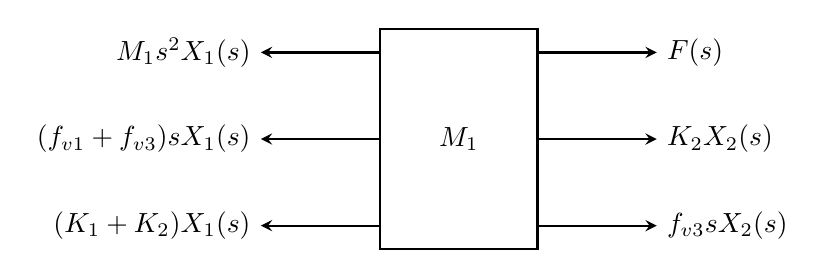
\begin{tikzpicture}[
    force/.style={->,>=stealth,thick}
]
    % Mass M1 block
    \node[draw, thick, minimum width=2cm, minimum height=2.8cm, label=center:$M_1$] (m1) {};

    % --- Left Arrows (Reaction Terms) on Left Side ---
    \draw[force] ([yshift=1.1cm]m1.west) -- ++(-1.5,0) node[left, left] {$M_1s^2X_1(s)$};
    \draw[force] ([yshift=0cm]m1.west) -- ++(-1.5,0) node[left, left] {$(f_{v1}+f_{v3})sX_1(s)$};
    \draw[force] ([yshift=-1.1cm]m1.west) -- ++(-1.5,0) node[left, left] {$(K_1+K_2)X_1(s)$};

    % --- Right Arrows (Input Terms) on Right Side ---
    \draw[force] ([yshift=1.1cm]m1.east) -- ++(1.5,0) node[right, right] {$F(s)$};
    \draw[force] ([yshift=0cm]m1.east) -- ++(1.5,0) node[right, right] {$K_2X_2(s)$};
    \draw[force] ([yshift=-1.1cm]m1.east) -- ++(1.5,0) node[right, right] {$f_{v3}sX_2(s)$};
    
\end{tikzpicture}
\end{figure}

The resulting equation in the Laplace domain is:
\begin{equation}
[M_1s^2 + (f_{v1} + f_{v3})s + (K_1 + K_2)]X_1(s) - (f_{v3}s + K_2)X_2(s) = F(s) \tag{1}
\end{equation}

\vspace{12pt}
{For Mass $M_2$:}
\begin{figure}[h!]
\centering
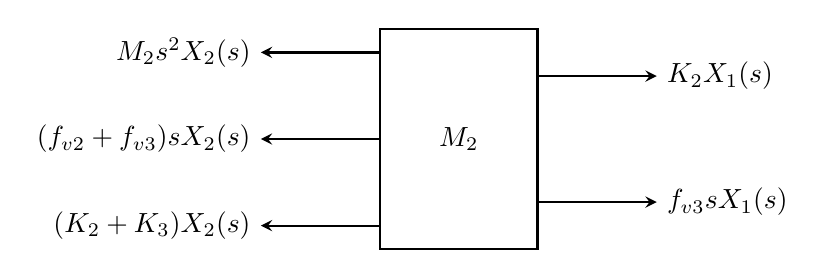
\begin{tikzpicture}[
    force/.style={->,>=stealth,thick}
]
    % Mass M2 block
    \node[draw, thick, minimum width=2cm, minimum height=2.8cm, label=center:$M_2$] (m2) {};

    % --- Left Arrows (Reaction Terms) on Left Side ---
    \draw[force] ([yshift=1.1cm]m2.west) -- ++(-1.5,0) node[left, left] {$M_2s^2X_2(s)$};
    \draw[force] ([yshift=0cm]m2.west) -- ++(-1.5,0) node[left, left] {$(f_{v2}+f_{v3})sX_2(s)$};
    \draw[force] ([yshift=-1.1cm]m2.west) -- ++(-1.5,0) node[left, left] {$(K_2+K_3)X_2(s)$};
    
    % --- Right Arrows (Input Terms) on Right Side ---
    \draw[force] ([yshift=0.8cm]m2.east) -- ++(1.5,0) node[right, right] {$K_2X_1(s)$};
    \draw[force] ([yshift=-0.8cm]m2.east) -- ++(1.5,0) node[right, right] {$f_{v3}sX_1(s)$};
    
\end{tikzpicture}
\end{figure}

The resulting equation in the Laplace domain is:
\begin{equation}
-(f_{v3}s + K_2)X_1(s) + [M_2s^2 + (f_{v2} + f_{v3})s + (K_2 + K_3)]X_2(s) = 0 \tag{2}
\end{equation}

\newpage
\noindent\textbf{Solving the System using Cramer's Rule}
\vspace{12pt}

The system can be expressed in matrix form $A\mathbf{x} = \mathbf{b}$:
$$
\begin{bmatrix}
Z_{1}(s) & -Z_{12}(s) \\
-Z_{12}(s) & Z_{2}(s)
\end{bmatrix}
\begin{bmatrix}
X_1(s) \\
X_2(s)
\end{bmatrix}
=
\begin{bmatrix}
F(s) \\
0
\end{bmatrix}
$$

where the mechanical impedances are:
\begin{align*}
    Z_{1}(s) &= M_1s^2 + (f_{v1} + f_{v3})s + (K_1 + K_2) \\
    Z_{2}(s) &= M_2s^2 + (f_{v2} + f_{v3})s + (K_2 + K_3) \\
    Z_{12}(s) &= f_{v3}s + K_2
\end{align*}

The solution for $X_2(s)$ is $G(s) = \frac{X_2(s)}{F(s)} = \frac{\det(A_2)}{\det(A)} = \frac{\Delta_2}{\Delta}$.

\vspace{12pt}
\noindent\textbf{Calculating the Numerator Determinant, $\Delta_2$}:
$$ \Delta_2 = \det
\begin{bmatrix}
Z_1(s) & F(s) \\
-Z_{12}(s) & 0
\end{bmatrix}
= Z_{12}(s)F(s) $$

{Calculating the Denominator Determinant, $\Delta$}:
$$\Delta = \det(A) = Z_1(s)Z_2(s) - Z_{12}(s)^2$$

{Constructing the Transfer Function}
$$G(s) = \frac{X_2(s)}{F(s)} = \frac{\Delta_2 / F(s)}{\Delta} = \frac{Z_{12}(s)}{Z_1(s)Z_2(s) - Z_{12}(s)^2}$$

Expanding the denominator yields the simplified standard form:
\[
\boxed{
G(s) = \frac{f_{v3}s + K_2}{[M_1s^2 + (f_{v1} + f_{v3})s + K_1 + K_2][M_2s^2 + (f_{v2} + f_{v3})s + K_2 + K_3] - (f_{v3}s + K_2)^2}
}
\]


% Problem 7 - Translational Mechanical System Transfer Functions

\newpage
% command for new page 
  \setcounter{page}{12}  
\noindent\rule{\textwidth}{1pt}
\noindent\textbf{Problem 7} \hfill 
%palagay ulit dito 'yung problem statement
\\ Find the transfer function, $G(s)=\frac{X_2(s)}{F(s)}$, of the given system below.


\begin{figure}[!ht]
\centering
\resizebox{0.8\textwidth}{!}{%
\begin{circuitikz}
\tikzstyle{every node}=[font=\large]


\draw[pattern=bricks, pattern color=black!60]
    (-0.75, 15.75) -- (-0.25, 15.75) -- (-0.25, 11.75) -- (11.75, 11.75)
    -- (11.75, 15.75) -- (12.25, 15.75) -- (12.25, 11.25) -- (-0.75, 11.25) -- cycle;


\draw (-0.25,12.75) to[L,l={ \large 1 N/m } ] (1.5,12.75);
\draw  (1.5,13.5) rectangle  node {\large 1 kg} (3,11.75);
\draw [short] (-0.25,15) -- (1.75,15);
\draw [short] (1.75,15.5) -- (1.75,14.5);
\draw [short] (1.75,14.5) -- (2.75,14.5);
\draw [short] (1.75,15.5) -- (2.75,15.5);
\draw [short] (2.25,15) -- (5.25,15);
\draw [short] (2.25,14.75) -- (2.25,15.25);
\draw [short] (3,12.75) -- (3.75,12.75);
\draw [short] (3.75,13.25) -- (3.75,12.25);
\draw [short] (6.25,13.25) -- (7,13.25);
\draw [short] (3.75,13.25) -- (4.75,13.25);
\draw [short] (4.25,12.75) -- (5.25,12.75);
\draw [short] (4.25,12.5) -- (4.25,13);
\draw  (5.25,15.5) rectangle  node {\large 1 kg} (6.25,11.75);
\draw [short] (3.75,12.25) -- (4.75,12.25);
\draw [short] (7,13.75) -- (7,12.75);
\draw [short] (7,12.75) -- (8,12.75);
\draw [short] (7,13.75) -- (8,13.75);
\draw [short] (7.5,13.25) -- (8.5,13.25);
\draw [short] (7.5,13) -- (7.5,13.5);
\draw (6.25,14.75) to[L ] (8.5,14.75);
\node [font=\large] at (7.25,14) {1 N-s/m};
\draw  (8.5,15.5) rectangle  node {\large 1 kg} (9.5,11.75);
\draw [short] (9.5,13.5) -- (10.25,13.5);
\draw [short] (10.25,14) -- (10.25,13);
\draw [short] (10.25,13) -- (11.25,13);
\draw [short] (10.25,14) -- (11.25,14);
\draw [short] (10.75,13.5) -- (11.75,13.5);
\draw [short] (10.75,13.25) -- (10.75,13.75);

% --- Labels and Arrows ---
\node [font=\large] at (2.25,15.75) {1 N-s/m};
\node [font=\large] at (7.5,15.25) {1 N/m };
\node [font=\large] at (4.25,13.5) {1 N-s/m};
\node [font=\large] at (10.5,14.25) {1 N-s/m};
\draw [ color={rgb,255:red,46; green,128; blue,163}, ->, >=Stealth] (2,14) -- (2.75,14);
\draw [ color={rgb,255:red,46; green,128; blue,163}, ->, >=Stealth] (6.25,12.25) -- (7.25,12.25);
\node [font=\large, color={rgb,255:red,46; green,128; blue,162}] at (7.75,12.25) {\textit{f(t)}};
\draw [ color={rgb,255:red,46; green,128; blue,163}, short] (2.25,13.25) -- (2.25,14.25);
\draw [ color={rgb,255:red,46; green,128; blue,163}, ->, >=Stealth] (5.5,16) -- (6.25,16);
\draw [ color={rgb,255:red,46; green,128; blue,163}, short] (5.75,15.25) -- (5.75,16.25);
\draw [ color={rgb,255:red,46; green,128; blue,163}, ->, >=Stealth] (8.75,16) -- (9.5,16);
\draw [ color={rgb,255:red,46; green,128; blue,163}, short] (9,15.25) -- (9,16.25);
\node [font=\large, color={rgb,255:red,46; green,128; blue,162}] at (3.5,14.25) {$x_1(t)$};
\node [font=\large, color={rgb,255:red,46; green,128; blue,162}] at (7,16.25) {$x_2(t)$};
\node [font=\large, color={rgb,255:red,46; green,128; blue,162}] at (10.25,16.25) {$x_3(t)$};
\draw [->, >=Stealth] (5.75,10.75) -- (5.75,11.75);
\draw [->, >=Stealth] (7,10.75) -- (9,11.75);
\draw [->, >=Stealth] (4.5,10.75) -- (2.25,11.75);
\node [font=\large] at (5.75,10.5) {Frictionless};
\end{circuitikz}
}%
\end{figure}


\noindent\rule{\textwidth}{1pt}

\vspace{12pt}


\noindent \textbf{\textit{Given:}} \ As per drawing

\vspace{12pt}

\noindent
\textbf{\textit{Required:}}
    \ Determine the transfer function:
    \[
    G(s) = \frac{X_2(s)}{F(s)}
    \]

\vspace{12pt}

\noindent \textbf{\textit{Solution:}}

\vspace{12 pt}

\noindent\textbf{Deriving the Equations of Motion}
\vspace{12pt}

\noindent We apply Newton's second law ($\sum F = ma$) to each mass to derive the system equations in the s-domain.
\vspace{12pt}
{For Mass M1:}
\begin{figure}[h!]
\centering
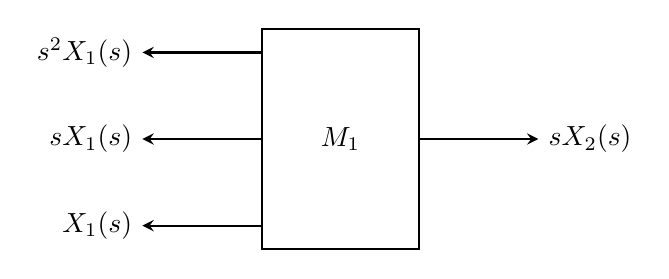
\begin{tikzpicture}[
    force/.style={->,>=stealth,thick}
]
    \node[draw, thick, minimum width=2cm, minimum height=2.8cm, label=center:$M_1$] (m1) {};
    % Left Arrows (Reaction Terms) - Separated
    \draw[force] ([yshift=1.1cm]m1.west) -- ++(-1.5,0) node[left, left] {$s^2X_1(s)$};
    \draw[force] ([yshift=0cm]m1.west) -- ++(-1.5,0) node[left, left] {$sX_1(s)$};
    \draw[force] ([yshift=-1.1cm]m1.west) -- ++(-1.5,0) node[left, left] {$X_1(s)$};
    % Right Arrow (Input Term)
    \draw[force] (m1.east) -- ++(1.5,0) node[right, right] {$sX_2(s)$};
\end{tikzpicture}
\end{figure}

The resulting equation in the Laplace domain is:
\begin{equation}
(s^2+s+1)X_1(s) - sX_2(s) = 0
\end{equation}

{For Mass M2:}
\begin{figure}[h!]
\centering
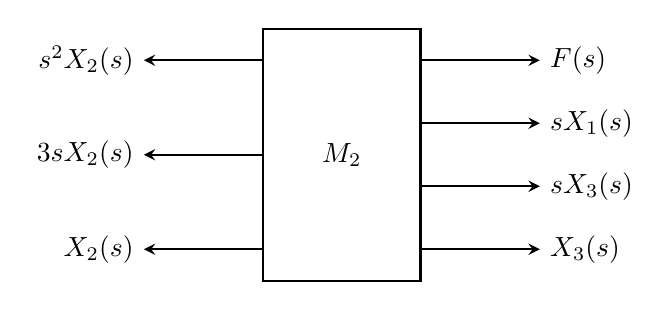
\begin{tikzpicture}[
    force/.style={->,>=stealth,thick}
]
    \node[draw, thick, minimum width=2cm, minimum height=3.2cm, label=center:$M_2$] (m2) {};
    % Left Arrows (Reaction Terms) - Separated
    \draw[force] ([yshift=1.2cm]m2.west) -- ++(-1.5,0) node[left,left] {$s^2X_2(s)$};
    \draw[force] ([yshift=0cm]m2.west) -- ++(-1.5,0) node[left,left] {$3sX_2(s)$};
    \draw[force] ([yshift=-1.2cm]m2.west) -- ++(-1.5,0) node[left,left] {$X_2(s)$};
    % Right Arrows (Input Terms) - Separated
    \draw[force] ([yshift=1.2cm]m2.east) -- ++(1.5,0) node[right,right] {$F(s)$};
    \draw[force] ([yshift=0.4cm]m2.east) -- ++(1.5,0) node[right,right] {$sX_1(s)$};
    \draw[force] ([yshift=-0.4cm]m2.east) -- ++(1.5,0) node[right,right] {$sX_3(s)$};
    \draw[force] ([yshift=-1.2cm]m2.east) -- ++(1.5,0) node[right,right] {$X_3(s)$};
\end{tikzpicture}
\end{figure}


The resulting equation in the Laplace domain is:
\begin{equation}
-sX_1(s) + (s^2+3s+1)X_2(s) - (s+1)X_3(s) = F(s)
\end{equation}

\newpage
{For Mass M3:}
\begin{figure}[h!]
\centering
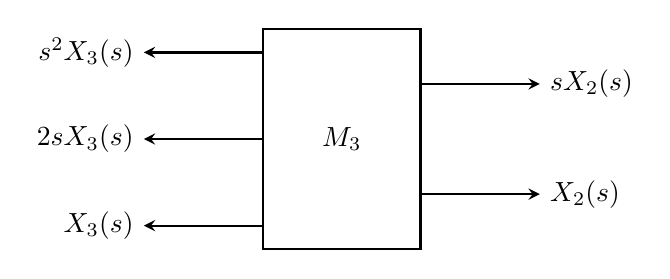
\begin{tikzpicture}[
    force/.style={->,>=stealth,thick}
]
    \node[draw, thick, minimum width=2cm, minimum height=2.8cm, label=center:$M_3$] (m3) {};
    % Left Arrows (Reaction Terms) - Separated
    \draw[force] ([yshift=1.1cm]m3.west) -- ++(-1.5,0) node[left,left] {$s^2X_3(s)$};
    \draw[force] ([yshift=0cm]m3.west) -- ++(-1.5,0) node[left,left] {$2sX_3(s)$};
    \draw[force] ([yshift=-1.1cm]m3.west) -- ++(-1.5,0) node[left,left] {$X_3(s)$};
    % Right Arrows (Input Terms) - Separated
    \draw[force] ([yshift=0.7cm]m3.east) -- ++(1.5,0) node[right,right] {$sX_2(s)$};
    \draw[force] ([yshift=-0.7cm]m3.east) -- ++(1.5,0) node[right,right] {$X_2(s)$};
\end{tikzpicture}
\end{figure}

The resulting equation in the Laplace domain is:
\begin{equation}
-(s+1)X_2(s) + (s^2+2s+1)X_3(s) = 0
\end{equation}

\noindent\textbf{Solving the System using Cramer's Rule}
\vspace{12pt}

The three system equations can be expressed in matrix form $A\mathbf{x} = \mathbf{b}$:
$$
\begin{bmatrix}
(s^2+s+1) & -s & 0 \\
-s & (s^2+3s+1) & -(s+1) \\
0 & -(s+1) & (s^2+2s+1)
\end{bmatrix}
\begin{bmatrix}
X_1(s) \\
X_2(s) \\
X_3(s)
\end{bmatrix}
=
\begin{bmatrix}
0 \\
F(s) \\
0
\end{bmatrix}
$$

The solution is $G(s) = \frac{X_2(s)}{F(s)} = \frac{\det(A_2)}{\det(A)} = \frac{\Delta_2}{\Delta}$.

\vspace{12pt}
\noindent\textbf{Calculating the Numerator Determinant, $\Delta_2$}:
$$ \Delta_2 = \det
\begin{bmatrix}
(s^2+s+1) & 0 & 0 \\
-s & F(s) & -(s+1) \\
0 & 0 & (s^2+2s+1)
\end{bmatrix}
= F(s)(s^2+s+1)(s+1)^2$$

\noindent\textbf{Calculating the Denominator Determinant, $\Delta$}:
$$\Delta = \det(A) = (s+1)^2 \left[ (s^2+s+1)(s^2+3s) + s^2 \right]$$

\vspace{12pt}
\noindent\textbf{Constructing and Simplifying the Transfer Function}
$$G(s) = \frac{\Delta_2 / F(s)}{\Delta} = \frac{(s^2+s+1)(s+1)^2}{(s+1)^2 \left[ (s^2+s+1)(s^2+3s) + s^2 \right]}$$

We cancel the common factor of $(s+1)^2$ to get:
$$G(s) = \frac{s^2+s+1}{(s^2+s+1)(s^2+3s) + s^2}$$

Finally, expanding the denominator gives the most simplified standard form:
\[
\boxed{
G(s) = \frac{s^2+s+1}{s^4 + 4s^3 + 5s^2 + 3s}
}
\]


% Problem 8 - Translational Mechanical System Transfer Functions

\newpage
% command for new page 
  \setcounter{page}{14}  
\noindent\rule{\textwidth}{1pt}
\noindent\textbf{Problem 8} \hfill 
%palagay ulit dito 'yung problem statement
\\ For the given system, find the transfer function $G(s)=\frac{X_1(s)}{F(s)}$.

\begin{figure}[!ht]
\centering
\resizebox{0.7\textwidth}{!}{%
\begin{circuitikz}

\tikzstyle{every node}=[font=\large]


\draw[pattern=bricks, pattern color=black!60] 
    (6, 12.5) -- (6, 15.75) -- (5.25, 15.75) -- (5.25, 11.5) -- (19.5, 11.5) 
    -- (19.5, 15.75) -- (18.75, 15.75) -- (18.75, 12.5) -- cycle;

\draw (6,14.75) to[L,l={\large $K_1 = 4\,\mathrm{N/m}$}] (9,14.75);
\draw (9,12.5) rectangle node {\large $M_1 = 1\,\mathrm{kg}$} (11,15.75);
\draw (11,13.25) to[short] (12,13.25);
\draw (12,13.25) to[short] (12,13.75);
\draw (12,13.75) to[short] (13,13.75);
\draw (12,13.25) to[short] (12,12.75);
\draw (12,12.75) to[short] (13,12.75);

\draw (11,14.75) to[L,l={\large $K_2 = 5\,\mathrm{N/m}$}] (14,14.75);
\draw (12.5,13.5) to[short] (12.5,13);
\draw (12.5,13.25) to[short] (14,13.25);
\draw (14,12.5) rectangle node {\large $M_2 = 2\,\mathrm{kg}$} (16,15.75);
\draw (16,14.75) to[L,l={\large $K_3 = 2\,\mathrm{N/m}$}] (18.75,14.75);

\draw [color={rgb,255:red,46; green,128; blue,163}, short] (10,15.75) -- (10,16.75);
\draw [color={rgb,255:red,46; green,128; blue,163},->,>=Stealth] (9.5,16.5) -- (10.75,16.5);
\draw [color={rgb,255:red,46; green,128; blue,163}, short] (15,15.75) -- (15,16.75);
\draw [color={rgb,255:red,46; green,128; blue,163},->,>=Stealth] (14.5,16.5) -- (15.75,16.5);
\draw [color={rgb,255:red,46; green,128; blue,163},->,>=Stealth] (16,15.75) -- (16.75,15.75);

\node [font=\Large, color={rgb,255:red,46; green,128; blue,163}] at (16.5,16.25) {$f(t)$};
\node [font=\Large, color={rgb,255:red,46; green,128; blue,163}] at (11,17) {$x_1(t)$};
\node [font=\Large, color={rgb,255:red,46; green,128; blue,163}] at (16,17) {$x_2(t)$};

\node [font=\normalsize] at (12.5,14) {$f_{v_2} = 3\,\mathrm{N\cdot s/m}$};

\draw [->, >=Stealth] (8.25,13.25) -- (9,12.5);
\node [font=\normalsize] at (7.5,13.5) {$f_{v_1} = 1\,\mathrm{N\cdot s/m}$};
\node [font=\normalsize] at (17.5,13.5) {$f_{v_3} = 2\,\mathrm{N\cdot s/m}$};
\draw [->, >=Stealth] (16.75,13.25) -- (16,12.5);

\end{circuitikz}
}
\end{figure}


\noindent\rule{\textwidth}{1pt}

\vspace{12pt}

\noindent\textbf{\textit{Given:}}
\[
M_1 = 1\, \text{kg}, \quad M_2 = 2\, \text{kg}
\]
\[
K_1 = 4\, \text{N/m}, \quad K_2 = 5\, \text{N/m}, \quad K_3 = 2\, \text{N/m}
\]
\[
f_{v_1} = 1\, \text{Ns/m}, \quad f_{v_2} = 3\, \text{Ns/m}, \quad f_{v_3} = 2\, \text{Ns/m}
\]
\vspace{12pt}

\noindent\textbf{\textit{Required:}}
\[
\text{Find the transfer function} \quad G(s) = \frac{X_1(s)}{F(s)}
\]


\noindent \textbf{\textit{Solution:}}

\vspace{12 pt}

\noindent\textbf{Deriving the Equations of Motion}
\vspace{12pt}

\noindent We apply Newton's second law ($\sum F = ma$) to each mass to derive the system equations in the s-domain. 
\vspace{12pt}
{For Mass M1:}
\begin{figure}[h!]
\centering
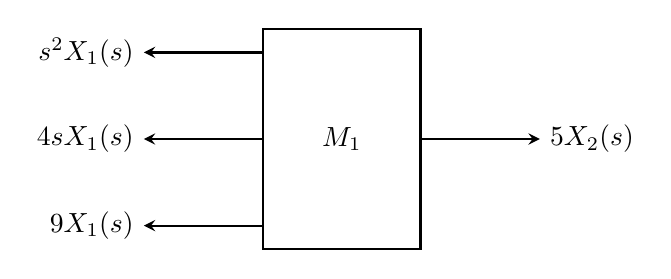
\begin{tikzpicture}[
    force/.style={->,>=stealth,thick}
]
    \node[draw, thick, minimum width=2cm, minimum height=2.8cm, label=center:$M_1$] (m1) {};
    % Left Arrows (Reaction Terms) - Now Separated
    \draw[force] ([yshift=1.1cm]m1.west) -- ++(-1.5,0) node[left,left] {$s^2X_1(s)$};
    \draw[force] ([yshift=0cm]m1.west) -- ++(-1.5,0) node[left,left] {$4sX_1(s)$};
    \draw[force] ([yshift=-1.1cm]m1.west) -- ++(-1.5,0) node[left,left] {$9X_1(s)$};
    % Right Arrow (Input Term)
    \draw[force] (m1.east) -- ++(1.5,0) node[right,right] {$5X_2(s)$};
\end{tikzpicture}
\end{figure}

The resulting equation in the Laplace domain is:
\begin{equation}
(s^2 + 4s + 9)X_1(s) - 5X_2(s) = 0 \tag{1}
\end{equation}

{For Mass M2:}
\begin{figure}[h!]
\centering
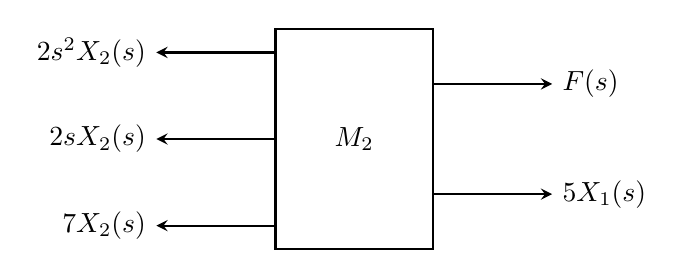
\begin{tikzpicture}[
    force/.style={->,>=stealth,thick}
]
    \node[draw, thick, minimum width=2cm, minimum height=2.8cm, label=center:$M_2$] (m2) {};
    % Left Arrows (Reaction Terms) - Now Separated
    \draw[force] ([yshift=1.1cm]m2.west) -- ++(-1.5,0) node[left,left] {$2s^2X_2(s)$};
    \draw[force] ([yshift=0cm]m2.west) -- ++(-1.5,0) node[left,left] {$2sX_2(s)$};
    \draw[force] ([yshift=-1.1cm]m2.west) -- ++(-1.5,0) node[left,left] {$7X_2(s)$};
    % Right Arrows (Input Terms)
    \draw[force] ([yshift=0.7cm]m2.east) -- ++(1.5,0) node[right,right] {$F(s)$};
    \draw[force] ([yshift=-0.7cm]m2.east) -- ++(1.5,0) node[right,right] {$5X_1(s)$};
\end{tikzpicture}
\end{figure}

The resulting equation in the Laplace domain is:
\begin{equation}
-5X_1(s) + (2s^2 + 2s + 7)X_2(s) = F(s) \tag{2}
\end{equation}

\newpage
\noindent\textbf{Solving the System using Cramer's Rule}
\vspace{12pt}

The two system equations can be expressed in matrix form $A\mathbf{x} = \mathbf{b}$:
$$
\begin{bmatrix}
s^2 + 4s + 9 & -5 \\
-5 & 2s^2 + 2s + 7
\end{bmatrix}
\begin{bmatrix}
X_1(s) \\
X_2(s)
\end{bmatrix}
=
\begin{bmatrix}
0 \\
F(s)
\end{bmatrix}
$$

The solution is $G(s) = \frac{X_1(s)}{F(s)} = \frac{\det(A_1)}{\det(A)} = \frac{\Delta_1}{\Delta}$.

\vspace{12pt}
\noindent\textbf{Calculating the Numerator Determinant, $\Delta_1$}:
\vspace{12pt}

We replace the first column of matrix $A$ with the vector $\mathbf{b}$.
$$ \Delta_1 = \det
\begin{bmatrix}
0 & -5 \\
F(s) & 2s^2 + 2s + 7
\end{bmatrix}
= (0)(2s^2 + 2s + 7) - (-5)F(s) = 5F(s) $$

\vspace{12pt}
\noindent\textbf{Calculating the Denominator Determinant, $\Delta$}:
$$\Delta = (s^2 + 4s + 9)(2s^2 + 2s + 7) - (-5)(-5)$$
$$\Delta = (2s^4 + 2s^3 + 7s^2 + 8s^3 + 8s^2 + 28s + 18s^2 + 18s + 63) - 25$$
$$\Delta = 2s^4 + 10s^3 + 33s^2 + 46s + 38$$

\vspace{12pt}
\noindent\textbf{Constructing the Transfer Function}
$$G(s) = \frac{X_1(s)}{F(s)} = \frac{\Delta_1 / F(s)}{\Delta}$$
\[
\boxed{
G(s) = \frac{5}{2s^4 + 10s^3 + 33s^2 + 46s + 38}
}
\]



% Problem 9 - Translational Mechanical System Transfer Functions

\newpage
% command for new page 
  \setcounter{page}{16}  
\noindent\rule{\textwidth}{1pt}
\noindent\textbf{Problem 9} \hfill 
%palagay ulit dito 'yung problem statement
\\ For the given system, find the transfer function $G(s)=\frac{X_3(s)}{F(s)}$.

\begin{figure}[!ht]
\centering
\resizebox{0.7\textwidth}{!}{%
\begin{circuitikz}
\tikzstyle{every node}=[font=\normalsize]


\draw[pattern=bricks, pattern color=black!60]
    (2, 22) -- (2.75, 22) -- (2.75, 17) -- (12.75, 17)
    -- (12.75, 16.25) -- (2, 16.25) -- cycle;


\node at (4.25,17.25) {$f_{v_2} = 3\,\mathrm{N\cdot s/m}$};
\draw (2.75,19.25) to[L,l={$K_1 = 5\,\mathrm{N/m}$}] (5.75,19.25);
\draw (5.75,17) rectangle node {$M_1 = 1\,\mathrm{kg}$} (7.75,20.25);

\draw (2.75,18) -- (3.75,18) -- (3.75,18.5) -- (4.75,18.5);
\draw (3.75,18) -- (3.75,17.5) -- (4.75,17.5);

\draw (7.75,18.75) to[L,l={$K_3 = 5\,\mathrm{N/m}$}] (10.75,18.75);
\draw (4.25,18.25) -- (4.25,17.75);
\draw (4.25,18) -- (5.75,18);
\draw (10.75,17) rectangle node {$M_2 = 2\,\mathrm{kg}$} (12.75,20.25);

\draw [color={rgb,255:red,46; green,128; blue,163},->,>=Stealth] (12.75,18.75) -- (13.5,18.75);
\node at (4.3,20.75) {$f_{v_1} = 2\,\mathrm{N\cdot s/m}$};

\draw (6.75,22) rectangle node {$M_3 = 4\,\mathrm{kg}$} (11.75,20.25);
\draw (2.75,21.25) to[L,l={$K_1 = 2\,\mathrm{N/m}$}] (6.75,21.25);

\draw [->, >=Stealth] (5.5,20.75) -- (6.75,20.25);
\draw [->, >=Stealth] (13,20.75) -- (11.75,20.25);

\draw (9.25,21.75) -- (9.25,23);
\draw [->, >=Stealth] (9,22.75) -- (10,22.75);
\node at (14.25,20.75) {$f_{v_3} = 2\,\mathrm{N\cdot s/m}$};
\node at (10.5,22.75) {$x_3(t)$};
\node at (13.75,18.75) {$f(t)$};

\draw (6.75,17) -- (8.75,17);
\draw (6.75,17) -- (6.75,15.5);
\draw [->, >=Stealth] (6.5,15.75) -- (7.25,15.75);

\draw (11.75,17) -- (11.75,15.5);
\draw [->, >=Stealth] (11.5,15.75) -- (12.25,15.75);
\draw [->, >=Stealth] (8.75,16) -- (7.75,17);
\node at (9.5,15.75) {Frictionless};
\draw [->, >=Stealth] (10,16) -- (10.75,17);

\node at (7.75,15.5) {$x_1(t)$};
\node at (12.5,15.5) {$x_2(t)$};

\end{circuitikz}
}
\end{figure}


\noindent\rule{\textwidth}{1pt}

\vspace{12pt}

\noindent\textbf{\textit{Given:}}
\[
M_1 = 1\,kg, \quad M_2 = 2\,kg, \quad M_3 = 4\,kg
\]
\[
K_1 = 2\,N/m, \quad K_2 = 5\,N/m, \quad K_3 = 5\,N/m
\]
\[
f_{v_1} = 2\,N\cdot s/m, \quad f_{v_2} = 3\,N\cdot s/m, \quad f_{v_3} = 2\,N\cdot s/m
\]

\vspace{12pt}

\noindent\textbf{\textit{Required:}}
Find the transfer function:
\[
G(s) = \frac{X_3(s)}{F(s)}
\]


\noindent \textbf{\textit{Solution:}}

\vspace{12 pt}

\noindent\textbf{Deriving the Equations of Motion}
\vspace{12pt}



\vspace{12pt}
{For Mass M1:}
\begin{figure}[h!]
\centering
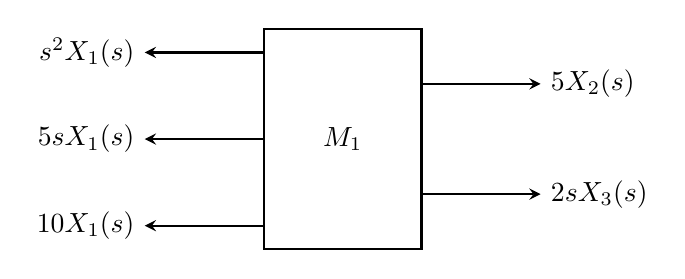
\begin{tikzpicture}[
    force/.style={->,>=stealth,thick}
]
    \node[draw, thick, minimum width=2cm, minimum height=2.8cm, label=center:$M_1$] (m1) {};
    % Left Arrows (Reaction Terms)
    \draw[force] ([yshift=1.1cm]m1.west) -- ++(-1.5,0) node[left,left] {$s^2X_1(s)$};
    \draw[force] ([yshift=0cm]m1.west) -- ++(-1.5,0) node[left,left] {$5sX_1(s)$};
    \draw[force] ([yshift=-1.1cm]m1.west) -- ++(-1.5,0) node[left,left] {$10X_1(s)$};
    % Right Arrows (Input Terms)
    \draw[force] ([yshift=0.7cm]m1.east) -- ++(1.5,0) node[right,right] {$5X_2(s)$};
    \draw[force] ([yshift=-0.7cm]m1.east) -- ++(1.5,0) node[right,right] {$2sX_3(s)$};
\end{tikzpicture}
\end{figure}

The resulting equation in the Laplace domain is:
\begin{equation}
(s^2 + 5s + 10)X_1(s) - 5X_2(s) - 2sX_3(s) = 0 \tag{1}
\end{equation}

\newpage
{For Mass M2:}
\begin{figure}[h!]
\centering
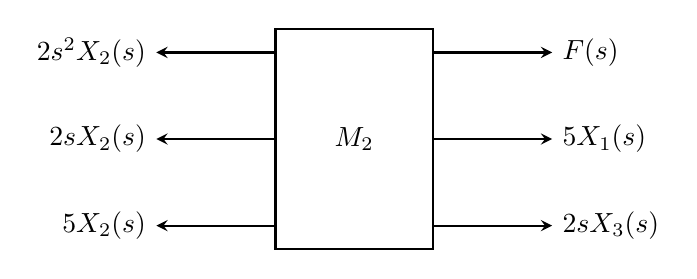
\begin{tikzpicture}[
    force/.style={->,>=stealth,thick}
]
    \node[draw, thick, minimum width=2cm, minimum height=2.8cm, label=center:$M_2$] (m2) {};
    % Left Arrows (Reaction Terms)
    \draw[force] ([yshift=1.1cm]m2.west) -- ++(-1.5,0) node[left,left] {$2s^2X_2(s)$};
    \draw[force] ([yshift=0cm]m2.west) -- ++(-1.5,0) node[left,left] {$2sX_2(s)$};
    \draw[force] ([yshift=-1.1cm]m2.west) -- ++(-1.5,0) node[left,left] {$5X_2(s)$};
    % Right Arrows (Input Terms)
    \draw[force] ([yshift=1.1cm]m2.east) -- ++(1.5,0) node[right,right] {$F(s)$};
    \draw[force] ([yshift=0cm]m2.east) -- ++(1.5,0) node[right,right] {$5X_1(s)$};
    \draw[force] ([yshift=-1.1cm]m2.east) -- ++(1.5,0) node[right,right] {$2sX_3(s)$};
\end{tikzpicture}
\end{figure}

The resulting equation in the Laplace domain is:
\begin{equation}
-5X_1(s) + (2s^2 + 2s + 5)X_2(s) - 2sX_3(s) = F(s) \tag{2}
\end{equation}

{For Mass M3:}
\begin{figure}[h!]
\centering
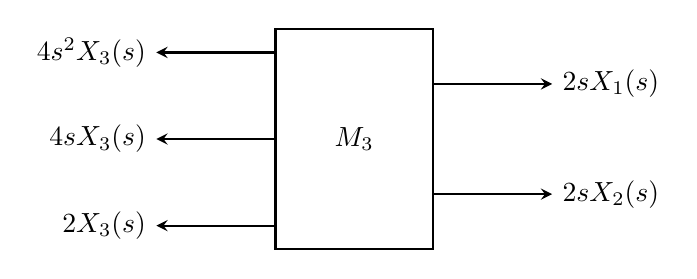
\begin{tikzpicture}[
    force/.style={->,>=stealth,thick}
]
    \node[draw, thick, minimum width=2cm, minimum height=2.8cm, label=center:$M_3$] (m3) {};
    % Left Arrows (Reaction Terms)
    \draw[force] ([yshift=1.1cm]m3.west) -- ++(-1.5,0) node[left,left] {$4s^2X_3(s)$};
    \draw[force] ([yshift=0cm]m3.west) -- ++(-1.5,0) node[left,left] {$4sX_3(s)$};
    \draw[force] ([yshift=-1.1cm]m3.west) -- ++(-1.5,0) node[left,left] {$2X_3(s)$};
    % Right Arrows (Input Terms)
    \draw[force] ([yshift=0.7cm]m3.east) -- ++(1.5,0) node[right,right] {$2sX_1(s)$};
    \draw[force] ([yshift=-0.7cm]m3.east) -- ++(1.5,0) node[right,right] {$2sX_2(s)$};
\end{tikzpicture}
\end{figure}

The resulting equation in the Laplace domain is:
\begin{equation}
-2sX_1(s) - 2sX_2(s) + (4s^2 + 4s + 2)X_3(s) = 0 \tag{3}
\end{equation}

\noindent\textbf{Solving the System using Cramer's Rule}
\vspace{12pt}

The three system equations can be expressed in matrix form $A\mathbf{x} = \mathbf{b}$:
$$
\begin{bmatrix}
s^2+5s+10 & -5 & -2s \\
-5 & 2s^2+2s+5 & -2s \\
-2s & -2s & 4s^2+4s+2
\end{bmatrix}
\begin{bmatrix}
X_1(s) \\
X_2(s) \\
X_3(s)
\end{bmatrix}
=
\begin{bmatrix}
0 \\
F(s) \\
0
\end{bmatrix}
$$

The solution is $G(s) = \frac{X_3(s)}{F(s)} = \frac{\det(A_3)}{\det(A)} = \frac{\Delta_3}{\Delta}$.

\vspace{12pt}
\noindent\textbf{Calculating the Numerator Determinant, $\Delta_3$}:
\vspace{12pt}

We replace the third column of matrix $A$ with the vector $\mathbf{b}$.
$$ \Delta_3 = \det
\begin{bmatrix}
s^2+5s+10 & -5 & 0 \\
-5 & 2s^2+2s+5 & F(s) \\
-2s & -2s & 0
\end{bmatrix}
= -F(s) \det \begin{vmatrix} s^2+5s+10 & -5 \\ -2s & -2s \end{vmatrix} $$
$$ \Delta_3 = -F(s) [-2s(s^2+5s+10) - (-5)(-2s)] = -F(s)[-2s^3 - 10s^2 - 20s - 10s] = F(s)(2s^3 + 10s^2 + 30s)$$

\vspace{12pt}
\noindent\textbf{Calculating the Denominator Determinant, $\Delta$}:
$$\Delta = 8s^6 + 56s^5 + 180s^4 + 316s^3 + 250s^2 + 190s + 50$$

\vspace{12pt}
\noindent\textbf{Constructing the Transfer Function}
$$G(s) = \frac{X_3(s)}{F(s)} = \frac{\Delta_3 / F(s)}{\Delta} = \frac{2s^3 + 10s^2 + 30s}{8s^6 + 56s^5 + 180s^4 + 316s^3 + 250s^2 + 190s + 50}$$

We can simplify by factoring out 2 from the numerator and denominator.
\[
\boxed{
G(s) = \frac{s^3 + 5s^2 + 15s}{4s^6 + 28s^5 + 90s^4 + 158s^3 + 125s^2 + 95s + 25}
}
\]

% Problem 10 - Translational Mechanical System Transfer Functions
\newpage
% command for new page 
  \setcounter{page}{18}  
\noindent\rule{\textwidth}{1pt}
\noindent\textbf{Problem 10} \hfill 
%palagay ulit dito 'yung problem statement
\\ For the given system, find the transfer function $G(s)=\frac{X_1(s)}{F(s)}$.



\begin{figure}[!ht]
\centering
\resizebox{0.9\textwidth}{!}{%
\begin{circuitikz}
\tikzstyle{every node}=[font=\large]


\draw[pattern=bricks, pattern color=black!60]
    (4.25, 13.25) -- (5, 13.25) -- (5, 7.75) -- (18.75, 7.75)
    -- (18.75, 7) -- (4.25, 7) -- cycle;


\draw [short] (2.25,7.25) -- (2.25,7.25); 
\draw (11.25,8.5) to[L ] (15,8.5);
\draw (8.75,7.75) rectangle node {\large $M_1 = 1\,\mathrm{kg}$} (11.25,10.75);
\draw (15,7.75) rectangle node {\large $M_2 = 2\,\mathrm{kg}$} (17.5,10.75);
\draw (10,10.75) rectangle node {\large $M_3 = 2\,\mathrm{kg}$} (16.25,13);
\draw [short] (5,12) -- (6.25,12);
\draw [short] (6.25,12.5) -- (7.5,12.5);
\draw [short] (6.25,11.5) -- (7.5,11.5);
\draw [short] (6.25,12.5) -- (6.25,11.5);
\draw [short] (7,12.25) -- (7,11.75);
\draw [short] (7,12) -- (10,12);
\draw [short] (5,9.5) -- (6.25,9.5);
\draw [short] (6.25,10) -- (7.5,10);
\draw [short] (6.25,9) -- (7.5,9);
\draw [short] (6.25,10) -- (6.25,9);
\draw [short] (7,9.25) -- (7,9.75);
\draw [short] (7,9.5) -- (8.75,9.5);
\draw [short] (11.25,10) -- (12.5,10);
\draw [short] (12.5,9.5) -- (13.5,9.5);
\draw [short] (12.5,10.5) -- (13.5,10.5);
\draw [short] (12.5,10.5) -- (12.5,9.5);
\draw [short] (13.25,10.25) -- (13.25,9.75);
\draw [short] (13.25,10) -- (15,10);
\draw [short] (13,13.75) -- (13,12.75);
\draw [->, >=Stealth] (12.5,13.5) -- (13.75,13.5);
\draw [->, >=Stealth] (18,11) -- (16.25,10.75);
\draw [->, >=Stealth] (17.5,9) -- (18.75,9);
\draw [->, >=Stealth] (8,11) -- (10,10.75);
\draw [->, >=Stealth] (11.75,6.75) -- (10.5,7.75);
\draw [->, >=Stealth] (14.25,6.75) -- (15.75,7.75);
\draw [short] (10,8) -- (10,6.25);
\draw [short] (16.25,8) -- (16.25,6.25);
\draw [->, >=Stealth] (9.25,6.5) -- (10.75,6.5);
\draw [->, >=Stealth] (15.5,6.5) -- (17,6.5);
\node [font=\normalsize] at (13,8) {K = 2 N/m};
\node [font=\large] at (14.25,13.5) {$x_3(t)$};
\node [font=\large] at (6.75,13) {$f_{v_3} = 1\,\mathrm{N\cdot s/m}$};
\node [font=\large] at (6.50,11) {$f_{v_4} = 1\,\mathrm{N\cdot s/m}$};
\node [font=\large] at (6.75,8.5) {$f_{v_1} = 1\,\mathrm{N\cdot s/m}$};
\node [font=\normalsize] at (13,9.25) {$f_{v_2} = 1\,\mathrm{N\cdot s/m}$};
\node [font=\large] at (19.5,11.25) {$f_{v_5} = 1\,\mathrm{N\cdot s/m}$};
\node [font=\large] at (19.25,9) {$f(t)$};
\node [font=\large] at (17.5,6.5) {$x_2(t)$};
\node [font=\large] at (11.25,6.5) {$x_1(t)$};
\node [font=\large] at (13,6.75) {Frictionless};
\end{circuitikz}
}
\end{figure}

\noindent\rule{\textwidth}{1pt}

\vspace{12pt}

\noindent\textbf{\textit{Given:}}

\[
M_1 = 1 \text{ kg}, \quad M_2 = 2 \text{ kg}, \quad M_3 = 2 \text{ kg}
\]
\[
K = 2 \text{ N/m}
\]
\[
f_{v_1} = f_{v_2} = f_{v_3} = f_{v_4} = 1 \text{ Ns/m}
\]

\vspace{12pt}

\noindent\textbf{\textit{Required:}}

\[
\text{Find the transfer function:} \quad G(s) = \frac{X_1(s)}{F(s)}
\]

\noindent \textbf{\textit{Solution:}}

\vspace{12 pt}

\noindent\textbf{Deriving the Equations of Motion}
\vspace{12pt}


\vspace{12pt}
{For Mass M1:}
\begin{figure}[h!]
\centering
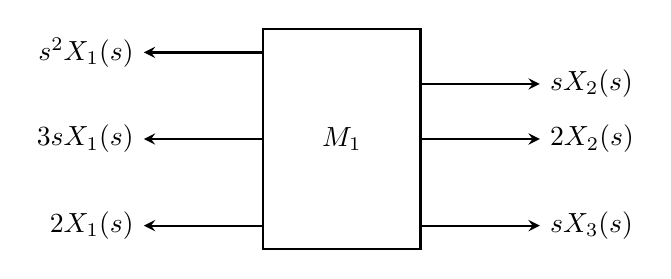
\begin{tikzpicture}[
    force/.style={->,>=stealth,thick}
]
    \node[draw, thick, minimum width=2cm, minimum height=2.8cm, label=center:$M_1$] (m1) {};
    % Left Arrows (Reaction Terms)
    \draw[force] ([yshift=1.1cm]m1.west) -- ++(-1.5,0) node[left,left] {$s^2X_1(s)$};
    \draw[force] ([yshift=0cm]m1.west) -- ++(-1.5,0) node[left,left] {$3sX_1(s)$};
    \draw[force] ([yshift=-1.1cm]m1.west) -- ++(-1.5,0) node[left,left] {$2X_1(s)$};
    % Right Arrows (Input Terms)
    \draw[force] ([yshift=0.7cm]m1.east) -- ++(1.5,0) node[right,right] {$sX_2(s)$};
    \draw[force] ([yshift=-0.0cm]m1.east) -- ++(1.5,0) node[right,right] {$2X_2(s)$};
    \draw[force] ([yshift=-1.1cm]m1.east) -- ++(1.5,0) node[right,right] {$sX_3(s)$};
\end{tikzpicture}
\end{figure}

The resulting equation in the Laplace domain is:
\begin{equation}
(s^2 + 3s + 2)X_1(s) - (s + 2)X_2(s) - sX_3(s) = 0 \tag{1}
\end{equation}

\newpage
{For Mass M2:}
\begin{figure}[h!]
\centering
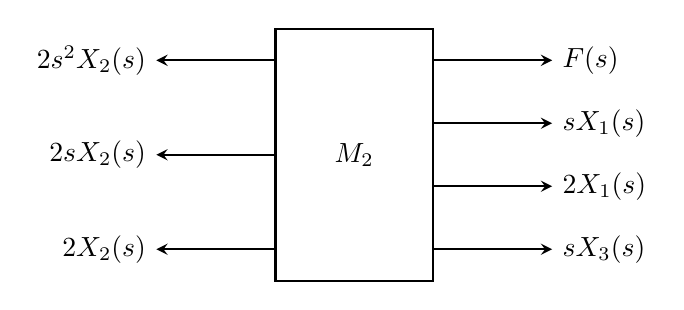
\begin{tikzpicture}[
    force/.style={->,>=stealth,thick}
]
    \node[draw, thick, minimum width=2cm, minimum height=3.2cm, label=center:$M_2$] (m2) {};
    % Left Arrows (Reaction Terms)
    \draw[force] ([yshift=1.2cm]m2.west) -- ++(-1.5,0) node[left,left] {$2s^2X_2(s)$};
    \draw[force] ([yshift=0cm]m2.west) -- ++(-1.5,0) node[left,left] {$2sX_2(s)$};
    \draw[force] ([yshift=-1.2cm]m2.west) -- ++(-1.5,0) node[left,left] {$2X_2(s)$};
    % Right Arrows (Input Terms)
    \draw[force] ([yshift=1.2cm]m2.east) -- ++(1.5,0) node[right,right] {$F(s)$};
    \draw[force] ([yshift=0.4cm]m2.east) -- ++(1.5,0) node[right,right] {$sX_1(s)$};
    \draw[force] ([yshift=-0.4cm]m2.east) -- ++(1.5,0) node[right,right] {$2X_1(s)$};
    \draw[force] ([yshift=-1.2cm]m2.east) -- ++(1.5,0) node[right,right] {$sX_3(s)$};
\end{tikzpicture}
\end{figure}

The resulting equation in the Laplace domain is:
\begin{equation}
-(s + 2)X_1(s) + (2s^2 + 2s + 2)X_2(s) - sX_3(s) = F(s) \tag{2}
\end{equation}

{For Mass M3:}
\begin{figure}[h!]
\centering
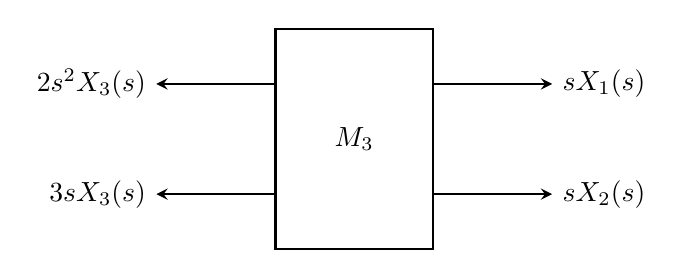
\begin{tikzpicture}[
    force/.style={->,>=stealth,thick}
]
    \node[draw, thick, minimum width=2cm, minimum height=2.8cm, label=center:$M_3$] (m3) {};
    % Left Arrows (Reaction Terms)
    \draw[force] ([yshift=0.7cm]m3.west) -- ++(-1.5,0) node[left,left] {$2s^2X_3(s)$};
    \draw[force] ([yshift=-0.7cm]m3.west) -- ++(-1.5,0) node[left,left] {$3sX_3(s)$};
    % Right Arrows (Input Terms)
    \draw[force] ([yshift=0.7cm]m3.east) -- ++(1.5,0) node[right,right] {$sX_1(s)$};
    \draw[force] ([yshift=-0.7cm]m3.east) -- ++(1.5,0) node[right,right] {$sX_2(s)$};
\end{tikzpicture}
\end{figure}


The resulting equation in the Laplace domain is:
\begin{equation}
-sX_1(s) - sX_2(s) + (2s^2 + 3s)X_3(s) = 0 \tag{3}
\end{equation}

\noindent\textbf{Solving the System using Cramer's Rule}
\vspace{12pt}

The three system equations can be expressed in matrix form $A\mathbf{x} = \mathbf{b}$:
$$
\begin{bmatrix}
s^2+3s+2 & -(s+2) & -s \\
-(s+2) & 2s^2+2s+2 & -s \\
-s & -s & 2s^2+3s
\end{bmatrix}
\begin{bmatrix}
X_1(s) \\
X_2(s) \\
X_3(s)
\end{bmatrix}
=
\begin{bmatrix}
0 \\
F(s) \\
0
\end{bmatrix}
$$

The solution is $G(s) = \frac{X_1(s)}{F(s)} = \frac{\det(A_1)}{\det(A)} = \frac{\Delta_1}{\Delta}$.

\vspace{12pt}
\noindent\textbf{Calculating the Numerator Determinant, $\Delta_1$}:
\vspace{12pt}

We replace the first column of matrix $A$ with the vector $\mathbf{b}$.
$$ \Delta_1 = \det
\begin{bmatrix}
0 & -(s+2) & -s \\
F(s) & 2s^2+2s+2 & -s \\
0 & -s & 2s^2+3s
\end{bmatrix}
= -F(s) \det \begin{vmatrix} -(s+2) & -s \\ -s & 2s^2+3s \end{vmatrix} $$
$$ \Delta_1 = -F(s) [-(s+2)(2s^2+3s) - s^2] = F(s)[(s+2)(2s^2+3s) + s^2] = F(s)(2s^3 + 7s^2 + 6s + s^2)$$
$$ \Delta_1 = F(s)(2s^3 + 8s^2 + 6s)$$

\vspace{12pt}
\noindent\textbf{Calculating the Denominator Determinant, $\Delta$}:
$$\Delta = 4s^6 + 22s^5 + 44s^4 + 42s^3 + 14s^2$$
$$\Delta = 2s^2(2s^4 + 11s^3 + 22s^2 + 21s + 7)$$

\vspace{12pt}
\noindent\textbf{Constructing the Transfer Function}
$$G(s) = \frac{X_1(s)}{F(s)} = \frac{\Delta_1 / F(s)}{\Delta} = \frac{2s^3 + 8s^2 + 6s}{2s^2(2s^4 + 11s^3 + 22s^2 + 21s + 7)}$$

We can simplify by factoring $2s$ from the numerator and denominator.
$$G(s) = \frac{2s(s^2 + 4s + 3)}{2s^2(2s^4 + 11s^3 + 22s^2 + 21s + 7)}$$
\[
\boxed{
G(s) = \frac{s^2 + 4s + 3}{s(2s^4 + 11s^3 + 22s^2 + 21s + 7)}
}
\]
% Problem 11 - Translational Mechanical System Transfer Functions
\newpage
% command for new page 
  \setcounter{page}{20}  
\noindent\rule{\textwidth}{1pt}
\noindent\textbf{Problem 11} \hfill 
%palagay ulit dito 'yung problem statement
\\ For the given system, find the transfer function $G(s)=\frac{X_2(s)}{F(s)}$.
\begin{figure}[!ht]
\centering
\resizebox{0.8\textwidth}{!}{%
\begin{circuitikz}
\tikzstyle{every node}=[font=\Large]

% --- NEW: Brick Wall and Base ---
% This single command replaces the 8 lines that previously drew the U-shaped frame.
\draw[pattern=bricks, pattern color=black!60]
    (-24.75, -12.75) -- (-23.75, -12.75) -- (-23.75, -20.25) -- (-1, -20.25)
    -- (-1, -12.75) -- (0, -12.75) -- (0, -21.75) -- (-24.75, -21.75) -- cycle;

% --- Original System Components (Frame-drawing lines removed) ---
\draw (-19,-13.75) rectangle node {\LARGE $M_1 = 2 kg$} (-14.25,-20.25);
\draw (-10,-13.75) rectangle node {\LARGE $M_2 = 3 kg$} (-5.25,-20.25);
\draw (-23.75,-17) to[L,l={ \Large $K_1 = 2 N/m$} ] (-19,-17);
\draw (-14.25,-15.5) to[L,l={ \Large $K_2 = 1 N/m$} ] (-10,-15.5);
\draw (-14.25,-19.75) to[L,l={ \Large $K_3 = 1 N/m$} ] (-10,-19.75);
\draw [short] (-14.25,-17.75) -- (-12.75,-17.75);
\draw [short] (-12.75,-17.25) -- (-11.5,-17.25);
\draw [short] (-12.75,-18.25) -- (-11.5,-18.25);
\draw [short] (-12,-17.75) -- (-10,-17.75);
\draw [short] (-12,-17.5) -- (-12,-18);
\draw [short] (-12.75,-17.25) -- (-12.75,-18.25);
\draw [->, >=Stealth] (-21,-14.5) -- (-19,-14.5);
\draw [->, >=Stealth] (-17.25,-12.5) -- (-15.25,-12.5);
\draw [->, >=Stealth] (-8,-12.5) -- (-6,-12.5);
\draw [->, >=Stealth] (-20,-19.25) -- (-19,-20.25);
\draw [short] (-16.75,-13.75) -- (-16.75,-12);
\draw [short] (-7.75,-13.75) -- (-7.75,-12);
\node [font=\Large] at (-21.5,-14.5) {f(t)};
\node [font=\Large] at (-14.5,-12.5) {$x_1(t)$};
\node [font=\Large] at (-5.25,-12.5) {$x_2(t)$};
\node [font=\Large] at (-21,-18.75) {$f_{v_1} = 1 N-s/m$};
\node [font=\Large] at (-12,-16.75) {$f_{v_2} = 1 N-s/m$};
\draw [short] (-5.25,-17) -- (-3.75,-17);
\draw [short] (-3.75,-16.5) -- (-2.5,-16.5);
\draw [short] (-3.75,-17.5) -- (-2.5,-17.5);
\draw [short] (-3,-17) -- (-1,-17);
\draw [short] (-3,-16.75) -- (-3,-17.25);
\draw [short] (-3.75,-16.5) -- (-3.75,-17.5);
\node [font=\Large] at (-3,-16) {$f_{v_3} = 1 N-s/m$};
\end{circuitikz}
}%
\end{figure}


\noindent\rule{\textwidth}{1pt}

\vspace{12pt}

\noindent\textbf{\textit{Given:}}

\[
M_1 = 2\, \text{kg}, \quad M_2 = 3\, \text{kg}
\]
\[
K_1 = 2\, \text{N/m}, \quad K_2 = 1\, \text{N/m}, \quad K_3 = 1\, \text{N/m}
\]
\[
f_{v_1} = f_{v_2} = f_{v_3} = 1\, \text{Ns/m}
\]

\vspace{12pt}

\noindent\textbf{\textit{Required:}}

\[
\text{Find the transfer function:} \quad G(s) = \frac{X_2(s)}{F(s)}
\]

\noindent \textbf{\textit{Solution:}}

\vspace{12 pt}

\noindent\textbf{Deriving the Equations of Motion}
\vspace{12pt}

\noindent We derive the system equations from the s-Domain Equation Diagrams below. 
\vspace{12pt}

{For Mass M1:}
\begin{figure}[h!]
\centering
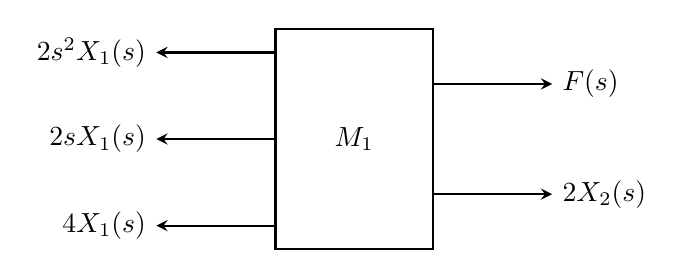
\begin{tikzpicture}[
    force/.style={->,>=stealth,thick}
]
    \node[draw, thick, minimum width=2cm, minimum height=2.8cm, label=center:$M_1$] (m1) {};
    % Left Arrows (Reaction Terms)
    \draw[force] ([yshift=1.1cm]m1.west) -- ++(-1.5,0) node[left,left] {$2s^2X_1(s)$};
    \draw[force] ([yshift=0cm]m1.west) -- ++(-1.5,0) node[left,left] {$2sX_1(s)$};
    \draw[force] ([yshift=-1.1cm]m1.west) -- ++(-1.5,0) node[left,left] {$4X_1(s)$};
    % Right Arrows (Input Terms)
    \draw[force] ([yshift=0.7cm]m1.east) -- ++(1.5,0) node[right,right] {$F(s)$};
    \draw[force] ([yshift=-0.7cm]m1.east) -- ++(1.5,0) node[right,right] {$2X_2(s)$};
\end{tikzpicture}
\end{figure}

The resulting equation in the Laplace domain is:
\begin{equation}
(2s^2 + 2s + 4)X_1(s) - 2X_2(s) = F(s) \tag{1}
\end{equation}

{For Mass M2:}
\begin{figure}[h!]
\centering
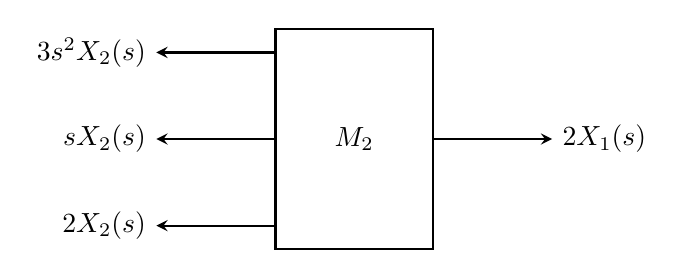
\begin{tikzpicture}[
    force/.style={->,>=stealth,thick}
]
    \node[draw, thick, minimum width=2cm, minimum height=2.8cm, label=center:$M_2$] (m2) {};
    % Left Arrows (Reaction Terms)
    \draw[force] ([yshift=1.1cm]m2.west) -- ++(-1.5,0) node[left,left] {$3s^2X_2(s)$};
    \draw[force] ([yshift=0cm]m2.west) -- ++(-1.5,0) node[left,left] {$sX_2(s)$};
    \draw[force] ([yshift=-1.1cm]m2.west) -- ++(-1.5,0) node[left,left] {$2X_2(s)$};
    % Right Arrows (Input Terms)
    \draw[force] (m2.east) -- ++(1.5,0) node[right,right] {$2X_1(s)$};
\end{tikzpicture}
\end{figure}


The resulting equation in the Laplace domain is:
\begin{equation}
-2X_1(s) + (3s^2 + s + 2)X_2(s) = 0 \tag{2}
\end{equation}

\newpage
\noindent\textbf{Solving the System using Cramer's Rule}
\vspace{12pt}

The two system equations can be expressed in matrix form $A\mathbf{x} = \mathbf{b}$:
$$
\begin{bmatrix}
2s^2 + 2s + 4 & -2 \\
-2 & 3s^2 + s + 2
\end{bmatrix}
\begin{bmatrix}
X_1(s) \\
X_2(s)
\end{bmatrix}
=
\begin{bmatrix}
F(s) \\
0
\end{bmatrix}
$$

The solution is $G(s) = \frac{X_2(s)}{F(s)} = \frac{\det(A_2)}{\det(A)} = \frac{\Delta_2}{\Delta}$.

\vspace{12pt}
\noindent\textbf{Calculating the Numerator Determinant, $\Delta_2$}:
\vspace{12pt}

We replace the second column of matrix $A$ with the vector $\mathbf{b}$.
$$ \Delta_2 = \det
\begin{bmatrix}
2s^2 + 2s + 4 & F(s) \\
-2 & 0
\end{bmatrix}
= (0)(2s^2 + 2s + 4) - (-2)F(s) = 2F(s) $$

\vspace{12pt}
\noindent\textbf{Calculating the Denominator Determinant, $\Delta$}:
$$\Delta = (2s^2 + 2s + 4)(3s^2 + s + 2) - (-2)(-2)$$
$$\Delta = (6s^4 + 2s^3 + 4s^2 + 6s^3 + 2s^2 + 4s + 12s^2 + 4s + 8) - 4$$
$$\Delta = 6s^4 + 8s^3 + 18s^2 + 8s + 4$$

\vspace{12pt}
\noindent\textbf{Constructing the Transfer Function}
$$G(s) = \frac{X_2(s)}{F(s)} = \frac{\Delta_2 / F(s)}{\Delta} = \frac{2}{6s^4 + 8s^3 + 18s^2 + 8s + 4}$$

We can simplify by factoring out 2 from the denominator.
\[
\boxed{
G(s) = \frac{1}{3s^4 + 4s^3 + 9s^2 + 4s + 2}
}
\]

% Problem 12 - Translational Mechanical System Transfer Functions
\newpage
% command for new page 
  \setcounter{page}{22}  
\noindent\rule{\textwidth}{1pt}
\noindent\textbf{Problem 12} \hfill 
%palagay ulit dito 'yung problem statement
\\ For the given system, find the transfer function $G(s)=\frac{X_1(s)}{F(s)}$.


\begin{figure}[!ht]
\centering
\resizebox{0.9\textwidth}{!}{%
\begin{circuitikz}
\tikzstyle{every node}=[font=\Large]

% --- NEW: Brick Wall and Base ---
% This single command replaces the 8 lines that previously drew the U-shaped frame.
\draw[pattern=bricks, pattern color=black!60]
    (-9.25, -5.25) -- (-8.25, -5.25) -- (-8.25, -12.75) -- (14.5, -12.75)
    -- (14.5, -5.25) -- (15.5, -5.25) -- (15.5, -14.25) -- (-9.25, -14.25) -- cycle;

% --- Original System Components (Frame-drawing lines removed) ---
\draw (-3.5,-6.25) rectangle node {\LARGE $M_1 = 1 kg$} (1.25,-12.75);
\draw (5.5,-6.25) rectangle node {\LARGE $M_2 = 1 kg$} (10.25,-12.75);
\draw (-8.25,-9.5) to[L,l={ \Large $K_1 = 1 N/m$} ] (-3.5,-9.5);
\draw (1.25,-8) to[L,l={ \Large $K_2 = 1 N/m$} ] (5.5,-8);
\draw (10.25,-9.25) to[L,l={ \Large $K_3 = 1 N/m$} ] (14.5,-9.25);
\draw [short] (1.25,-11) -- (2.75,-11);
\draw [short] (2.75,-10.5) -- (4,-10.5);
\draw [short] (2.75,-11.5) -- (4,-11.5);
\draw [short] (3.5,-11) -- (5.5,-11);
\draw [short] (3.5,-10.75) -- (3.5,-11.25);
\draw [short] (2.75,-10.5) -- (2.75,-11.5);
\draw [->, >=Stealth] (-5.5,-7) -- (-3.5,-7);
\draw [->, >=Stealth] (-1.75,-5) -- (0.25,-5);
\draw [->, >=Stealth] (7.5,-5) -- (9.5,-5);
\draw [->, >=Stealth] (-4.5,-11.75) -- (-3.5,-12.75);
\draw [->, >=Stealth] (11.25,-11.75) -- (10.25,-12.75);
\draw [short] (-1.25,-6.25) -- (-1.25,-4.5);
\draw [short] (7.75,-6.25) -- (7.75,-4.5);
\node [font=\Large] at (-6,-7) {f(t)};
\node [font=\Large] at (1,-5) {$x_1(t)$};
\node [font=\Large] at (10.25,-5) {$x_2(t)$};
\node [font=\Large] at (-5.5,-11.25) {$f_{v_1} = 1 N-s/m$};
\node [font=\Large] at (12.5,-11) {$f_{v_3} = 1 N-s/m$};
\node [font=\Large] at (3.5,-10) {$f_{v_2} = 1 N-s/m$};
\end{circuitikz}
}%
\end{figure}

\noindent\rule{\textwidth}{1pt}


\vspace{12pt}

\noindent\textbf{\textit{Given:}}

\[
M_1 = 1\, \text{kg}, \quad M_2 = 1\, \text{kg}
\]
\[
K_1 = K_2 = K_3 = 1\, \text{N/m}
\]
\[
f_{v_1} = f_{v_2} = f_{v_3} = 1\, \text{Ns/m}
\]


\vspace{12pt}

\noindent\textbf{\textit{Required:}}

\[
\text{Find the transfer function:} \quad G(s) = \frac{X_1(s)}{F(s)}
\]

\noindent \textbf{\textit{Solution:}}

\vspace{12 pt}

\noindent\textbf{Deriving the Equations of Motion}
\vspace{12pt}

\noindent We derive the system equations from the s-Domain Equation Diagrams below. 
\vspace{12pt}

{For Mass M1:}
\begin{figure}[h!]
\centering
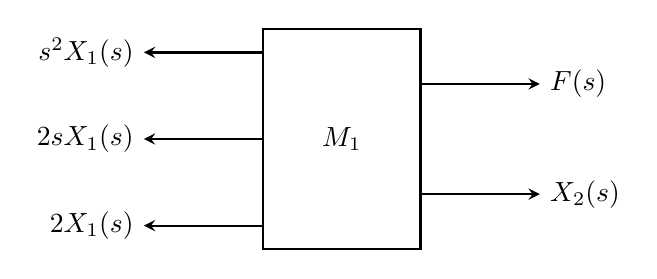
\begin{tikzpicture}[
    force/.style={->,>=stealth,thick}
]
    \node[draw, thick, minimum width=2cm, minimum height=2.8cm, label=center:$M_1$] (m1) {};
    % Left Arrows (Reaction Terms)
    \draw[force] ([yshift=1.1cm]m1.west) -- ++(-1.5,0) node[left,left] {$s^2X_1(s)$};
    \draw[force] ([yshift=0cm]m1.west) -- ++(-1.5,0) node[left,left] {$2sX_1(s)$};
    \draw[force] ([yshift=-1.1cm]m1.west) -- ++(-1.5,0) node[left,left] {$2X_1(s)$};
    % Right Arrows (Input Terms)
    \draw[force] ([yshift=0.7cm]m1.east) -- ++(1.5,0) node[right,right] {$F(s)$};
    \draw[force] ([yshift=-0.7cm]m1.east) -- ++(1.5,0) node[right,right] {$X_2(s)$};
\end{tikzpicture}
\end{figure}

The resulting equation in the Laplace domain is:
\begin{equation}
(s^2 + 2s + 2)X_1(s) - X_2(s) = F(s) \tag{1}
\end{equation}

{For Mass M2:}
\begin{figure}[h!]
\centering
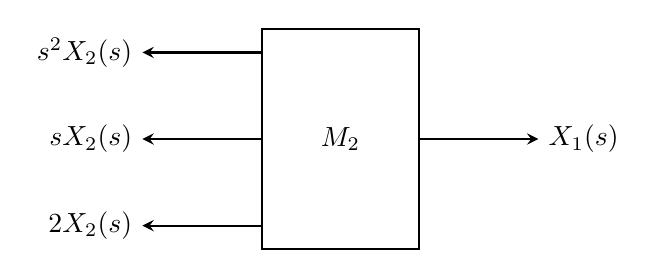
\begin{tikzpicture}[
    force/.style={->,>=stealth,thick}
]
    \node[draw, thick, minimum width=2cm, minimum height=2.8cm, label=center:$M_2$] (m2) {};
    % Left Arrows (Reaction Terms)
    \draw[force] ([yshift=1.1cm]m2.west) -- ++(-1.5,0) node[left,left] {$s^2X_2(s)$};
    \draw[force] ([yshift=0cm]m2.west) -- ++(-1.5,0) node[left,left] {$sX_2(s)$};
    \draw[force] ([yshift=-1.1cm]m2.west) -- ++(-1.5,0) node[left,left] {$2X_2(s)$};
    % Right Arrow (Input Term)
    \draw[force] (m2.east) -- ++(1.5,0) node[right,right] {$X_1(s)$};
\end{tikzpicture}
\end{figure}


The resulting equation in the Laplace domain is:
\begin{equation}
-X_1(s) + (s^2 + s + 2)X_2(s) = 0 \tag{2}
\end{equation}

\newpage
\noindent\textbf{Solving the System using Cramer's Rule}
\vspace{12pt}

The two system equations can be expressed in matrix form $A\mathbf{x} = \mathbf{b}$:
$$
\begin{bmatrix}
s^2 + 2s + 2 & -1 \\
-1 & s^2 + s + 2
\end{bmatrix}
\begin{bmatrix}
X_1(s) \\
X_2(s)
\end{bmatrix}
=
\begin{bmatrix}
F(s) \\
0
\end{bmatrix}
$$

The solution is $G(s) = \frac{X_1(s)}{F(s)} = \frac{\det(A_1)}{\det(A)} = \frac{\Delta_1}{\Delta}$.

\vspace{12pt}
\noindent\textbf{Calculating the Numerator Determinant, $\Delta_1$}:
\vspace{12pt}

We replace the first column of matrix $A$ with the vector $\mathbf{b}$.
$$ \Delta_1 = \det
\begin{bmatrix}
F(s) & -1 \\
0 & s^2 + s + 2
\end{bmatrix}
= F(s)(s^2 + s + 2) - (0)(-1) = F(s)(s^2 + s + 2) $$

\vspace{12pt}
\noindent\textbf{Calculating the Denominator Determinant, $\Delta$}:
$$\Delta = (s^2 + 2s + 2)(s^2 + s + 2) - (-1)(-1)$$
$$\Delta = (s^4 + s^3 + 2s^2 + 2s^3 + 2s^2 + 4s + 2s^2 + 2s + 4) - 1$$
$$\Delta = s^4 + 3s^3 + 6s^2 + 6s + 3$$

\vspace{12pt}
\noindent\textbf{Constructing the Transfer Function}
$$G(s) = \frac{X_1(s)}{F(s)} = \frac{\Delta_1 / F(s)}{\Delta}$$
\[
\boxed{
G(s) = \frac{s^2 + s + 2}{s^4 + 3s^3 + 6s^2 + 6s + 3}
}
\]
% Problem 13 - Translational Mechanical System Transfer Functions
\newpage
% command for new page 
  \setcounter{page}{24}  
\noindent\rule{\textwidth}{1pt}
\noindent\textbf{Problem 13} \hfill 
%palagay ulit dito 'yung problem statement
\\ For the given system, find the transfer function $G(s)=\frac{X_1(s)}{F(s)}$.

\begin{figure}[!ht]
\centering
\resizebox{0.9\textwidth}{!}{%
\begin{circuitikz}
\tikzstyle{every node}=[font=\LARGE]


\draw[pattern=bricks, pattern color=black!60]
    (-14.5, -7.75) -- (-13.5, -7.75) -- (-13.5, -19.75) -- (13.5, -19.75)
    -- (13.5, -21) -- (-14.5, -21) -- cycle;

\draw (-8,-14.5) rectangle node {\huge $M_1 = 2 kg$} (-2,-19.75);
\draw (6,-14.5) rectangle node {\huge $M_2 = 2 kg$} (11.75,-19.75);
\draw (-5.5,-9) rectangle node {\huge $M_3 = 1 kg$} (9.25,-14.5);
\draw (-13.5,-17.25) to[L,l={ \LARGE $K_1 = 1 N/m$} ] (-8,-17.25);
\draw [line width=0.5pt](-2,-17.25) to[L,l={ \LARGE $K_2 = 5 N/m$} ] (6,-17.25);
\draw [->, >=Stealth] (-4.75,-21.5) .. controls (-3.25,-20) and (-4.75,-18.5) .. (-5.25,-19.5) ;
\draw [->, >=Stealth] (9,-21.5) .. controls (10.5,-20) and (9,-18.5) .. (8.5,-19.5) ;
\draw [->, >=Stealth] (0.25,-7.25) -- (3.5,-7.25);
\draw [->, >=Stealth] (10.25,-13.25) -- (12.25,-13.25);
\draw [->, >=Stealth] (-4.75,-13.25) -- (-2.5,-13.25);
\draw [->, >=Stealth] (-7.25,-13) -- (-5.5,-14.5);
\draw [->, >=Stealth] (7.25,-13) -- (9.25,-14.5);
\draw [->, >=Stealth] (11.75,-17.25) -- (14,-17.25);
\draw [short] (1,-6.5) -- (1,-9.5);
\draw [short] (-4.5,-12.75) -- (-4.5,-15);
\draw [short] (10.5,-12.75) -- (10.5,-15);
\node [font=\LARGE] at (-8.25,-12.5) {$f_{v_3} = 1 N-s/m$};
\node [font=\LARGE] at (5.5,-13) {$f_{v_4} = 1 N-s/m$};
\node [font=\LARGE] at (-5.25,-22) {$f_{v_1} = 2 N-s/m$};
\node [font=\LARGE] at (9,-22) {$f_{v_2} = 1 N-s/m$};
\node [font=\LARGE] at (4.5,-7.25) {$x_3(t)$};
\node [font=\LARGE] at (-1.75,-13.25) {$x_1(t)$};
\node [font=\LARGE] at (13.25,-13.25) {$x_2(t)$};
\node [font=\LARGE] at (14.75,-17.25) {$f(t)$};
\end{circuitikz}
}%
\end{figure}



\noindent\rule{\textwidth}{1pt}

\vspace{12pt}

\noindent\textbf{\textit{Given}}

\[
M_1 = 2\, \text{kg}, \quad M_2 = 2\, \text{kg}, \quad M_3 = 1\, \text{kg}
\]
\[
K_1 = 1\, \text{N/m}, \quad K_2 = 5\, \text{N/m}
\]
\[
f_{v_1} = 2\, \text{Ns/m}, \quad f_{v_2} = 1\, \text{Ns/m}, \quad f_{v_3} = 1\, \text{Ns/m}, \quad f_{v_4} = 1\, \text{Ns/m}
\]


\noindent\textbf{\textit{Required}}
\[
G(s) = \frac{X_1(s)}{F(s)}
\]

\noindent \textbf{\textit{Solution:}}

\vspace{12 pt}

\noindent\textbf{Deriving the Equations of Motion}
\vspace{12pt}

\noindent We derive the system equations from the s-Domain Equation Diagrams below. The diagrams are based on the final Laplace equations, with each arrow representing an individual term corresponding to inertia, damping, or spring stiffness.

\vspace{12pt}
{For Mass M1:}
\begin{figure}[h!]
\centering
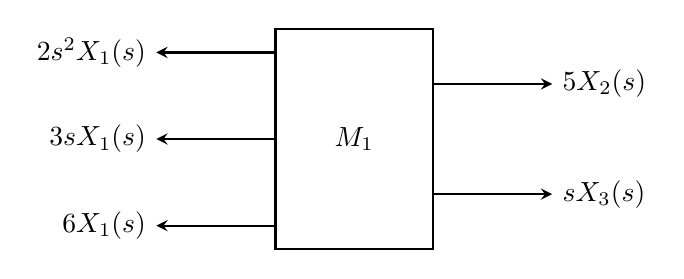
\begin{tikzpicture}[
    force/.style={->,>=stealth,thick}
]
    \node[draw, thick, minimum width=2cm, minimum height=2.8cm, label=center:$M_1$] (m1) {};
    % Left Arrows (Reaction Terms)
    \draw[force] ([yshift=1.1cm]m1.west) -- ++(-1.5,0) node[left,left] {$2s^2X_1(s)$};
    \draw[force] ([yshift=0cm]m1.west) -- ++(-1.5,0) node[left,left] {$3sX_1(s)$};
    \draw[force] ([yshift=-1.1cm]m1.west) -- ++(-1.5,0) node[left,left] {$6X_1(s)$};
    % Right Arrows (Input Terms)
    \draw[force] ([yshift=0.7cm]m1.east) -- ++(1.5,0) node[right,right] {$5X_2(s)$};
    \draw[force] ([yshift=-0.7cm]m1.east) -- ++(1.5,0) node[right,right] {$sX_3(s)$};
\end{tikzpicture}
\end{figure}

The resulting equation in the Laplace domain is:
\begin{equation}
(2s^2 + 3s + 6)X_1(s) - 5X_2(s) - sX_3(s) = 0 \tag{1}
\end{equation}

\newpage
{For Mass M2:}
\begin{figure}[h!]
\centering
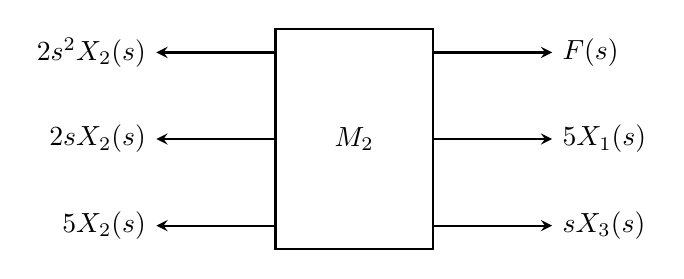
\begin{tikzpicture}[
    force/.style={->,>=stealth,thick}
]
    \node[draw, thick, minimum width=2cm, minimum height=2.8cm, label=center:$M_2$] (m2) {};
    % Left Arrows (Reaction Terms)
    \draw[force] ([yshift=1.1cm]m2.west) -- ++(-1.5,0) node[left,left] {$2s^2X_2(s)$};
    \draw[force] ([yshift=0cm]m2.west) -- ++(-1.5,0) node[left,left] {$2sX_2(s)$};
    \draw[force] ([yshift=-1.1cm]m2.west) -- ++(-1.5,0) node[left,left] {$5X_2(s)$};
    % Right Arrows (Input Terms)
    \draw[force] ([yshift=1.1cm]m2.east) -- ++(1.5,0) node[right,right] {$F(s)$};
    \draw[force] ([yshift=0cm]m2.east) -- ++(1.5,0) node[right,right] {$5X_1(s)$};
    \draw[force] ([yshift=-1.1cm]m2.east) -- ++(1.5,0) node[right,right] {$sX_3(s)$};
\end{tikzpicture}
\end{figure}

The resulting equation in the Laplace domain is:
\begin{equation}
-5X_1(s) + (2s^2 + 2s + 5)X_2(s) - sX_3(s) = F(s) \tag{2}
\end{equation}

{For Mass M3:}
\begin{figure}[h!]
\centering
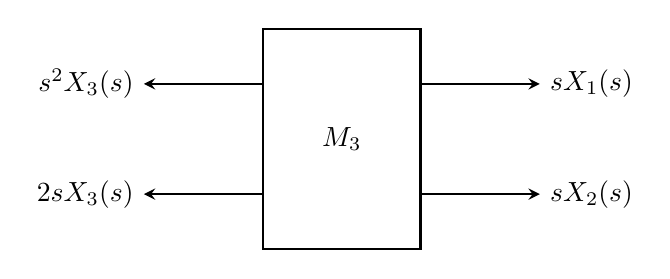
\begin{tikzpicture}[
    force/.style={->,>=stealth,thick}
]
    \node[draw, thick, minimum width=2cm, minimum height=2.8cm, label=center:$M_3$] (m3) {};
    % Left Arrows (Reaction Terms)
    \draw[force] ([yshift=0.7cm]m3.west) -- ++(-1.5,0) node[left,left] {$s^2X_3(s)$};
    \draw[force] ([yshift=-0.7cm]m3.west) -- ++(-1.5,0) node[left,left] {$2sX_3(s)$};
    % Right Arrows (Input Terms)
    \draw[force] ([yshift=0.7cm]m3.east) -- ++(1.5,0) node[right,right] {$sX_1(s)$};
    \draw[force] ([yshift=-0.7cm]m3.east) -- ++(1.5,0) node[right,right] {$sX_2(s)$};
\end{tikzpicture}
\end{figure}


The resulting equation in the Laplace domain is:
\begin{equation}
-sX_1(s) - sX_2(s) + (s^2 + 2s)X_3(s) = 0 \tag{3}
\end{equation}

\noindent\textbf{Solving the System using Cramer's Rule}
\vspace{12pt}

The three system equations can be expressed in matrix form $A\mathbf{x} = \mathbf{b}$:
$$
\begin{bmatrix}
2s^2 + 3s + 6 & -5 & -s \\
-5 & 2s^2 + 2s + 5 & -s \\
-s & -s & s^2 + 2s
\end{bmatrix}
\begin{bmatrix}
X_1(s) \\
X_2(s) \\
X_3(s)
\end{bmatrix}
=
\begin{bmatrix}
0 \\
F(s) \\
0
\end{bmatrix}
$$

The solution is $G(s) = \frac{X_1(s)}{F(s)} = \frac{\det(A_1)}{\det(A)} = \frac{\Delta_1}{\Delta}$.

\vspace{12pt}
\noindent\textbf{Calculating the Numerator Determinant, $\Delta_1$}:
\vspace{12pt}

We replace the first column of matrix $A$ with the vector $\mathbf{b}$.
$$ \Delta_1 = \det
\begin{bmatrix}
0 & -5 & -s \\
F(s) & 2s^2 + 2s + 5 & -s \\
0 & -s & s^2 + 2s
\end{bmatrix}
= -F(s) \det \begin{vmatrix} -5 & -s \\ -s & s^2+2s \end{vmatrix} $$
$$ \Delta_1 = -F(s) [-5(s^2+2s) - (-s)(-s)] = -F(s)[-5s^2 - 10s - s^2] = F(s)(6s^2 + 10s)$$

\vspace{12pt}
\noindent\textbf{Calculating the Denominator Determinant, $\Delta$}:
$$\Delta = s(4s^5 + 18s^4 + 44s^3 + 78s^2 + 38s + 10) = 2s(2s^5 + 9s^4 + 22s^3 + 39s^2 + 19s + 5)$$

\vspace{12pt}
\noindent\textbf{Constructing the Transfer Function}
$$G(s) = \frac{X_1(s)}{F(s)} = \frac{\Delta_1 / F(s)}{\Delta} = \frac{6s^2 + 10s}{2s(2s^5 + 9s^4 + 22s^3 + 39s^2 + 19s + 5)}$$

We can simplify by factoring out $2s$ from the numerator and denominator.
$$G(s) = \frac{2s(3s + 5)}{2s(2s^5 + 9s^4 + 22s^3 + 39s^2 + 19s + 5)}$$
\[
\boxed{
G(s) = \frac{3s + 5}{2s^5 + 9s^4 + 22s^3 + 39s^2 + 19s + 5}
}
\]
% Problem 14 - Translational Mechanical System Transfer Functions
\newpage
  \setcounter{page}{26}  
\noindent\rule{\textwidth}{1pt}
\noindent\textbf{Problem 14} \hfill 
\\ For the given system, find the transfer function $G(s)=\frac{X_1(s)}{F(s)}$.


\begin{figure}[!ht]
\centering
\resizebox{0.9\textwidth}{!}{%
\begin{circuitikz}
\tikzstyle{every node}=[font=\Large]


% Top wall
\filldraw[pattern=bricks, pattern color=black!60] (-11.25, 9.5) rectangle (7.5, 9);
% Bottom wall
\filldraw[pattern=bricks, pattern color=black!60] (-11.25, 1.25) rectangle (7.5, 0.75);
% Left wall
\filldraw[pattern=bricks, pattern color=black!60] (-11.25, 9) rectangle (-10.75, 1.25);
% Right wall
\filldraw[pattern=bricks, pattern color=black!60] (7, 9) rectangle (7.5, 1.25);

\draw (-6.5,4.75) rectangle node {\Large $M_1 = 2\, \text{kg}$} (2,1.25);
\draw (-5.5,9) rectangle node {\Large $M_2 = 1\, \text{kg}$} (-0.5,4.75);
\draw (-10.75,6.75) to[L] (-5.5,6.75);
\draw (2,3.25) to[L] (7,3.25);

\draw [short] (-4,8.5) -- (-4,10.75);
\draw [->, >=Stealth] (-4.75,10.25) -- (-2.5,10.25);
\draw [short] (3.5,9.25) -- (3.5,11);
\draw [->, >=Stealth] (2.75,10.5) -- (5,10.5);
\draw [short] (0.75,4.25) -- (0.75,5.5);
\draw [->, >=Stealth] (0.25,5.25) -- (2,5.25);
\draw [->, >=Stealth] (0.5,7.75) -- (-0.5,9);
\draw [->, >=Stealth] (0.5,6.25) -- (-0.5,4.75);
\draw [->, >=Stealth] (2.75,1.75) -- (2,1.25);
\draw [->, >=Stealth] (-12.75,5.25) -- (-11.25,5.25);

\node at (2.25,7.75) {$f_{v_1} = 1\, \text{N$\cdot$s/m}$};
\node at (2.25,6.25) {$f_{v_2} = 1\, \text{N$\cdot$s/m}$};
\node at (2.75,5.25) {$x_1(t)$};
\node at (4.5,4) {$K_2 = 1\, \text{N/m}$};
\node at (4.5,2) {$f_{v_3} = 1\, \text{N$\cdot$s/m}$};
\node at (-1.75,10.25) {$x_2(t)$};
\node at (5.75,10.5) {$x_3(t)$};
\node at (-8,7.5) {$K_1 = 1\, \text{N/m}$};
\node at (0.25,9.75) {$M_3 = 1\, \text{kg}$};
\node at (-13.5,5.25) {$f(t)$};
\end{circuitikz}
}
\end{figure}

\noindent\rule{\textwidth}{1pt}

\vspace{12pt}


\noindent\textbf{\textit{Given:}}
\[
M_1 = 2\, \text{kg}, \quad M_2 = 1\, \text{kg}, \quad M_3 = 1\, \text{kg}
\]
\[
K_1 = K_2 = 1\, \text{N/m}
\]
\[
f_{v_1} = f_{v_2} = f_{v_3} = 1\, \text{Ns/m}
\]
\[
\text{External force: } F(t) \text{ is applied}
\]

\noindent\textbf{\textit{Required:}}
\[
G(s) = \frac{X_1(s)}{F(s)}
\]

\noindent \textbf{\textit{Solution:}}

\vspace{12 pt}

\noindent\textbf{Deriving the Equations of Motion}
\vspace{12pt}

\noindent We derive the system equations from the s-Domain Equation Diagrams below. 
\vspace{12pt}

{For Mass M1:}
\begin{figure}[h!]
\centering
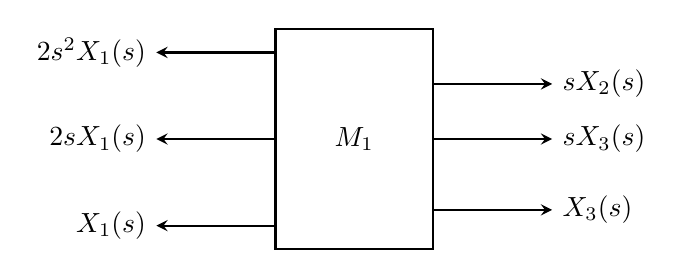
\begin{tikzpicture}[
    force/.style={->,>=stealth,thick}
]
    \node[draw, thick, minimum width=2cm, minimum height=2.8cm, label=center:$M_1$] (m1) {};
    % Left Arrows (Reaction Terms)
    \draw[force] ([yshift=1.1cm]m1.west) -- ++(-1.5,0) node[left,left] {$2s^2X_1(s)$};
    \draw[force] ([yshift=0cm]m1.west) -- ++(-1.5,0) node[left,left] {$2sX_1(s)$};
    \draw[force] ([yshift=-1.1cm]m1.west) -- ++(-1.5,0) node[left,left] {$X_1(s)$};
    % Right Arrows (Input Terms)
    \draw[force] ([yshift=0.7cm]m1.east) -- ++(1.5,0) node[right,right] {$sX_2(s)$};
    \draw[force] ([yshift=-0.0cm]m1.east) -- ++(1.5,0) node[right,right] {$sX_3(s)$};
    \draw[force] ([yshift=-0.9cm]m1.east) -- ++(1.5,0) node[right,right] {$X_3(s)$};
\end{tikzpicture}
\end{figure}

The resulting equation in the Laplace domain is:
\begin{equation}
(2s^2 + 2s + 1)X_1(s) - sX_2(s) - (s+1)X_3(s) = 0 \tag{1}
\end{equation}

{For Mass M2:}
\begin{figure}[h!]
\centering
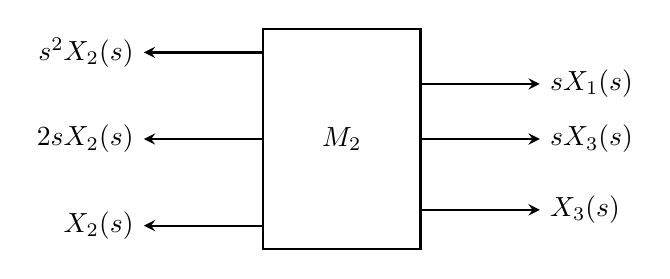
\begin{tikzpicture}[
    force/.style={->,>=stealth,thick}
]
    \node[draw, thick, minimum width=2cm, minimum height=2.8cm, label=center:$M_2$] (m2) {};
    % Left Arrows (Reaction Terms)
    \draw[force] ([yshift=1.1cm]m2.west) -- ++(-1.5,0) node[left,left] {$s^2X_2(s)$};
    \draw[force] ([yshift=0cm]m2.west) -- ++(-1.5,0) node[left,left] {$2sX_2(s)$};
    \draw[force] ([yshift=-1.1cm]m2.west) -- ++(-1.5,0) node[left,left] {$X_2(s)$};
    % Right Arrows (Input Terms)
    \draw[force] ([yshift=0.7cm]m2.east) -- ++(1.5,0) node[right,right] {$sX_1(s)$};
    \draw[force] ([yshift=-0.0cm]m2.east) -- ++(1.5,0) node[right,right] {$sX_3(s)$};
    \draw[force] ([yshift=-0.9cm]m2.east) -- ++(1.5,0) node[right,right] {$X_3(s)$};
\end{tikzpicture}
\end{figure}

The resulting equation in the Laplace domain is:
\begin{equation}
-sX_1(s) + (s^2 + 2s + 1)X_2(s) - (s+1)X_3(s) = 0 \tag{2}
\end{equation}

{For Mass M3:}
\begin{figure}[h!]
\centering
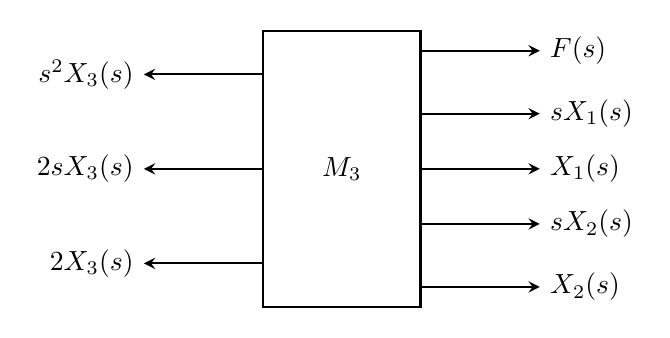
\begin{tikzpicture}[
    force/.style={->,>=stealth,thick}
]
    \node[draw, thick, minimum width=2cm, minimum height=3.5cm, label=center:$M_3$] (m3) {};
    % Left Arrows (Reaction Terms)
    \draw[force] ([yshift=1.2cm]m3.west) -- ++(-1.5,0) node[left,left] {$s^2X_3(s)$};
    \draw[force] ([yshift=0cm]m3.west) -- ++(-1.5,0) node[left,left] {$2sX_3(s)$};
    \draw[force] ([yshift=-1.2cm]m3.west) -- ++(-1.5,0) node[left,left] {$2X_3(s)$};
    % Right Arrows (Input Terms)
    \draw[force] ([yshift=1.5cm]m3.east) -- ++(1.5,0) node[right,right] {$F(s)$};
    \draw[force] ([yshift=0.7cm]m3.east) -- ++(1.5,0) node[right,right] {$sX_1(s)$};
    \draw[force] ([yshift=0cm]m3.east) -- ++(1.5,0) node[right,right] {$X_1(s)$};
    \draw[force] ([yshift=-0.7cm]m3.east) -- ++(1.5,0) node[right,right] {$sX_2(s)$};
    \draw[force] ([yshift=-1.5cm]m3.east) -- ++(1.5,0) node[right,right] {$X_2(s)$};
\end{tikzpicture}
\end{figure}

The resulting equation in the Laplace domain is:
\begin{equation}
-(s+1)X_1(s) - (s+1)X_2(s) + (s^2 + 2s + 2)X_3(s) = F(s) \tag{3}
\end{equation}

\noindent\textbf{Solving the System using Cramer's Rule}
\vspace{12pt}

The three system equations can be expressed in matrix form $A\mathbf{x} = \mathbf{b}$:
$$
\begin{bmatrix}
2s^2 + 2s + 1 & -s & -(s + 1) \\
-s & (s+1)^2 & -(s + 1) \\
-(s+1) & -(s+1) & s^2 + 2s + 2
\end{bmatrix}
\begin{bmatrix}
X_1(s) \\
X_2(s) \\
X_3(s)
\end{bmatrix}
=
\begin{bmatrix}
0 \\
0 \\
F(s)
\end{bmatrix}
$$

The solution is $G(s) = \frac{X_1(s)}{F(s)} = \frac{\det(A_1)}{\det(A)} = \frac{\Delta_1}{\Delta}$.

\vspace{12pt}
\noindent\textbf{Calculating the Numerator Determinant, $\Delta_1$}:
\vspace{12pt}

We replace the first column of matrix $A$ with the vector $\mathbf{b}$.
$$ \Delta_1 = \det
\begin{bmatrix}
0 & -s & -(s + 1) \\
0 & (s+1)^2 & -(s + 1) \\
F(s) & -(s+1) & s^2 + 2s + 2
\end{bmatrix}
= F(s) \det \begin{vmatrix} -s & -(s+1) \\ (s+1)^2 & -(s+1) \end{vmatrix} $$
$$ \Delta_1 = F(s) [(-s)(-(s+1)) - (-(s+1))((s+1)^2)] = F(s)[s(s+1) + (s+1)^3] $$
$$ \Delta_1 = F(s)(s+1)[s + (s+1)^2] = F(s)(s+1)(s^2+3s+1) $$

\vspace{12pt}
\noindent\textbf{Calculating the Denominator Determinant, $\Delta$}:
$$ \Delta = s^2(2s^4 + 10s^3 + 19s^2 + 16s + 4) $$

\vspace{12pt}
\noindent\textbf{Constructing the Transfer Function}
$$G(s) = \frac{X_1(s)}{F(s)} = \frac{\Delta_1 / F(s)}{\Delta}$$
\[
\boxed{
G(s) = \frac{(s+1)(s^2+3s+1)}{s^2(2s^4 + 10s^3 + 19s^2 + 16s + 4)}
}
\]

% Problem 15 - Translational Mechanical System Transfer Functions
\newpage
% command for new page 
  \setcounter{page}{28}  
\noindent\rule{\textwidth}{1pt}
\noindent\textbf{Problem 15} \hfill 
%palagay ulit dito 'yung problem statement
\\ For the given system, find the transfer function $G(s)=\frac{X_1(s)}{F(s)}$.

\begin{figure}[!ht]
\centering
\resizebox{0.9\textwidth}{!}{%
\begin{circuitikz}
\tikzstyle{every node}=[font=\Large]

\draw[pattern=bricks, pattern color=black!60]
    (-21.75, -14.75) -- (-20.75, -14.75) -- (-20.75, -26.75) -- (9.25, -26.75)
    -- (9.25, -28) -- (-21.75, -28) -- cycle;

\draw (-17,-17.25) rectangle node {\Large $M_1 = 1 kg$} (-11.5,-26.75);
\draw (-7.5,-17.25) rectangle node {\Large $M_2 = 2 kg$} (-2,-26.75);
\draw (1.75,-17.25) rectangle node {\Large $M_3 = 1 kg$} (7.25,-26.75);
\draw (-20.75,-20.25) to[L,l={ \Large $K_1 = 1 N/m$} ] (-17,-20.25);
\draw (-11.5,-20.25) to[L,l={ \Large $K_2 = 1 N/m$} ] (-7.5,-20.25);
\draw (-2,-20.25) to[L,l={ \Large $K_3 = 1 N/m$} ] (1.75,-20.25);
\draw [short] (-2,-22.75) -- (-0.25,-22.75);
\draw [short] (-0.25,-22.5) -- (-0.25,-23);
\draw [short] (-0.75,-22.25) -- (0.25,-22.25);
\draw [short] (0.25,-22.25) -- (0.25,-23.25);
\draw [short] (-0.75,-23.25) -- (0.25,-23.25);
\draw [short] (0.25,-22.75) -- (1.75,-22.75);
\draw [short] (-20.75,-22.75) -- (-19,-22.75);
\draw [short] (-19,-22.5) -- (-19,-23);
\draw [short] (-19.5,-22.25) -- (-18.5,-22.25);
\draw [short] (-18.5,-22.25) -- (-18.5,-23.25);
\draw [short] (-19.5,-23.25) -- (-18.5,-23.25);
\draw [short] (-18.5,-22.75) -- (-17,-22.75);
\draw [short] (-11.5,-22.75) -- (-9.5,-22.75);
\draw [short] (-9.5,-22.5) -- (-9.5,-23);
\draw [short] (-10,-22.25) -- (-9,-22.25);
\draw [short] (-9,-22.25) -- (-9,-23.25);
\draw [short] (-10,-23.25) -- (-9,-23.25);
\draw [short] (-9,-22.75) -- (-7.5,-22.75);
\draw [->, >=Stealth] (-15.25,-16) -- (-13,-16);
\draw [short] (-14.5,-15.5) -- (-14.5,-17.25);
\draw [->, >=Stealth] (-6,-16) -- (-3.75,-16);
\draw [short] (-5.25,-15.5) -- (-5.25,-17.25);
\draw [->, >=Stealth] (3.25,-16) -- (5.5,-16);
\draw [short] (4,-15.5) -- (4,-17.25);
\node [font=\Large] at (-12,-16) {$x_1(t)$};
\node [font=\Large] at (-2.75,-16) {$x_2(t)$};
\node [font=\Large] at (6.5,-16) {$x_3(t)$};
\node [font=\Large] at (-18.75,-24) {$f_{v_1} = 1 N-s/m$};
\node [font=\Large] at (-9.25,-24) {$f_{v_2} = 1 N-s/m$};
\node [font=\Large] at (0,-24) {$f_{v_3} = 1 N-s/m$};
\draw [->, >=Stealth] (7.25,-21.75) -- (9,-21.75);
\node [font=\Large] at (9.75,-21.75) {$f(t)$};
\end{circuitikz}
}%
\end{figure}

\noindent\rule{\textwidth}{1pt}

\vspace{12pt}

\noindent\textbf{\textit{Given:}}
\[
M_1 = 1\, \text{kg}, \quad M_2 = 2\, \text{kg}, \quad M_3 = 1\, \text{kg}
\]
\[
K_1 = K_2 = K_3 = 1\, \text{N/m}
\]
\[
f_{v1} = f_{v2} = f_{v3} = 1\, \text{Ns/m}
\]
\[\text {External force } F(t) \text { is applied to } M_3
\]



\vspace{12pt}

\noindent\textbf{\textit{Required:}}
\[
G(s) = \frac{X_1(s)}{F(s)}
\]

\noindent \textbf{\textit{Solution:}}

\vspace{12 pt}

\noindent\textbf{Deriving the Equations of Motion}
\vspace{12pt}

\noindent We derive the system equations from the s-Domain Equation Diagrams below. 

\vspace{12pt}

{For Mass M1:}
\begin{figure}[h!]
\centering
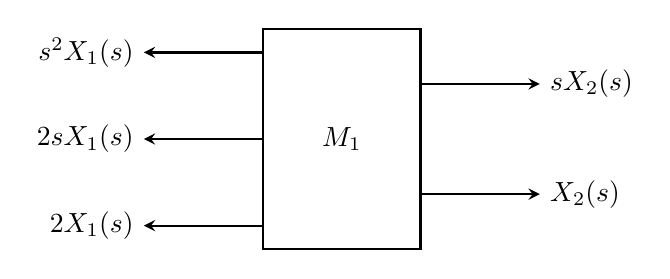
\begin{tikzpicture}[
    force/.style={->,>=stealth,thick}
]
    \node[draw, thick, minimum width=2cm, minimum height=2.8cm, label=center:$M_1$] (m1) {};
    % Left Arrows (Reaction Terms)
    \draw[force] ([yshift=1.1cm]m1.west) -- ++(-1.5,0) node[left,left] {$s^2X_1(s)$};
    \draw[force] ([yshift=0cm]m1.west) -- ++(-1.5,0) node[left,left] {$2sX_1(s)$};
    \draw[force] ([yshift=-1.1cm]m1.west) -- ++(-1.5,0) node[left,left] {$2X_1(s)$};
    % Right Arrows (Input Terms)
    \draw[force] ([yshift=0.7cm]m1.east) -- ++(1.5,0) node[right,right] {$sX_2(s)$};
    \draw[force] ([yshift=-0.7cm]m1.east) -- ++(1.5,0) node[right,right] {$X_2(s)$};
\end{tikzpicture}
\end{figure}

The resulting equation in the Laplace domain is:
\begin{equation}
(s^2 + 2s + 2)X_1(s) - (s+1)X_2(s) = 0 \tag{1}
\end{equation}

{For Mass M2:}
\begin{figure}[h!]
\centering
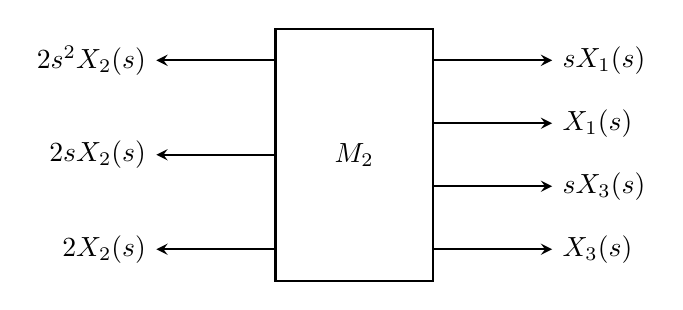
\begin{tikzpicture}[
    force/.style={->,>=stealth,thick}
]
    \node[draw, thick, minimum width=2cm, minimum height=3.2cm, label=center:$M_2$] (m2) {};
    % Left Arrows (Reaction Terms)
    \draw[force] ([yshift=1.2cm]m2.west) -- ++(-1.5,0) node[left,left] {$2s^2X_2(s)$};
    \draw[force] ([yshift=0cm]m2.west) -- ++(-1.5,0) node[left,left] {$2sX_2(s)$};
    \draw[force] ([yshift=-1.2cm]m2.west) -- ++(-1.5,0) node[left,left] {$2X_2(s)$};
    % Right Arrows (Input Terms)
    \draw[force] ([yshift=1.2cm]m2.east) -- ++(1.5,0) node[right,right] {$sX_1(s)$};
    \draw[force] ([yshift=0.4cm]m2.east) -- ++(1.5,0) node[right,right] {$X_1(s)$};
    \draw[force] ([yshift=-0.4cm]m2.east) -- ++(1.5,0) node[right,right] {$sX_3(s)$};
    \draw[force] ([yshift=-1.2cm]m2.east) -- ++(1.5,0) node[right,right] {$X_3(s)$};
\end{tikzpicture}
\end{figure}

The resulting equation in the Laplace domain is:
\begin{equation}
-(s+1)X_1(s) + (2s^2 + 2s + 2)X_2(s) - (s+1)X_3(s) = 0 \tag{2}
\end{equation}
\newpage
{For Mass M3:}
\begin{figure}[h!]
\centering
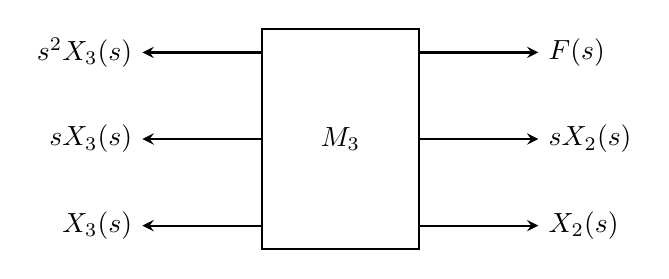
\begin{tikzpicture}[
    force/.style={->,>=stealth,thick}
]
    \node[draw, thick, minimum width=2cm, minimum height=2.8cm, label=center:$M_3$] (m3) {};
    % Left Arrows (Reaction Terms)
    \draw[force] ([yshift=1.1cm]m3.west) -- ++(-1.5,0) node[left,left] {$s^2X_3(s)$};
    \draw[force] ([yshift=0cm]m3.west) -- ++(-1.5,0) node[left,left] {$sX_3(s)$};
    \draw[force] ([yshift=-1.1cm]m3.west) -- ++(-1.5,0) node[left,left] {$X_3(s)$};
    % Right Arrows (Input Terms)
    \draw[force] ([yshift=1.1cm]m3.east) -- ++(1.5,0) node[right,right] {$F(s)$};
    \draw[force] ([yshift=0cm]m3.east) -- ++(1.5,0) node[right,right] {$sX_2(s)$};
    \draw[force] ([yshift=-1.1cm]m3.east) -- ++(1.5,0) node[right,right] {$X_2(s)$};
\end{tikzpicture}
\end{figure}

The resulting equation in the Laplace domain is:
\begin{equation}
-(s+1)X_2(s) + (s^2 + s + 1)X_3(s) = F(s) \tag{3}
\end{equation}

\noindent\textbf{Solving the System using Cramer's Rule}
\vspace{12pt}

The three system equations can be expressed in matrix form $A\mathbf{x} = \mathbf{b}$:
$$
\begin{bmatrix}
s^2 + 2s + 2 & -(s+1) & 0 \\
-(s+1) & 2s^2 + 2s + 2 & -(s+1) \\
0 & -(s+1) & s^2 + s + 1
\end{bmatrix}
\begin{bmatrix}
X_1(s) \\
X_2(s) \\
X_3(s)
\end{bmatrix}
=
\begin{bmatrix}
0 \\
0 \\
F(s)
\end{bmatrix}
$$

The solution is $G(s) = \frac{X_1(s)}{F(s)} = \frac{\det(A_1)}{\det(A)} = \frac{\Delta_1}{\Delta}$.

\vspace{12pt}
\noindent\textbf{Calculating the Numerator Determinant, $\Delta_1$}:
\vspace{12pt}

We replace the first column of matrix $A$ with the vector $\mathbf{b}$.
$$ \Delta_1 = \det
\begin{bmatrix}
0 & -(s+1) & 0 \\
0 & 2s^2 + 2s + 2 & -(s+1) \\
F(s) & -(s+1) & s^2 + s + 1
\end{bmatrix}
= F(s) \det \begin{vmatrix} -(s+1) & 0 \\ 2s^2+2s+2 & -(s+1) \end{vmatrix} $$
$$ \Delta_1 = F(s) (s+1)^2 $$

\vspace{12pt}
\noindent\textbf{Calculating the Denominator Determinant, $\Delta$}:
$$ \Delta = (s^2+2s+2)\big( (2s^2+2s+2)(s^2+s+1) - (s+1)^2 \big) - (-(s+1))\big( (-(s+1))(s^2+s+1) \big) $$
$$ \Delta = 2s^6 + 8s^5 + 16s^4 + 17s^3 + 11s^2 + 3s + 1 $$

\vspace{12pt}
\noindent\textbf{Constructing the Transfer Function}
$$ G(s) = \frac{X_1(s)}{F(s)} = \frac{\Delta_1 / F(s)}{\Delta} = \frac{(s+1)^2}{\Delta} $$
\[
\boxed{
G(s) = \frac{s^2 + 2s + 1}{2s^6 + 8s^5 + 16s^4 + 17s^3 + 11s^2 + 3s + 1} 
}
\]

% Problem 16 - Rotational Mechanical System Transfer Functions
\newpage
  \setcounter{page}{30}  
\noindent\rule{\textwidth}{1pt}
\noindent\textbf{Problem 16} \hfill 
\\ For the given system, find the transfer function $\frac{\theta_1(s)}{T(s)}$.

\begin{figure}[!ht]
\centering
\resizebox{0.8\textwidth}{!}{%
\begin{circuitikz}
\tikzstyle{every node}=[font=\small]


\filldraw[pattern=bricks, pattern color=black!60] (2.75,30) rectangle (3.5,26.25);
\filldraw[pattern=bricks, pattern color=black!60] (15.75,30) rectangle (16.5,26.25);

\draw (5.5,28) ellipse (0.25cm and 0.75cm);
\draw [short] (5.5,28.75) -- (8.25,28.75);
\draw [short] (5.5,27.25) -- (8.25,27.25);
\draw (10.5,28) ellipse (0.25cm and 0.75cm);
\draw [short] (10.5,28.75) -- (13.25,28.75);
\draw [short] (10.5,27.25) -- (13.25,27.25);
\draw (8.5,28.5) to[short] (9,28.5);
\draw (9,28.5) to[short] (9,29);
\draw (9,29) to[short] (10,29);
\draw (9,28.5) to[short] (9,28);
\draw (9,28) to[short] (10,28);
\draw (9.5,28.75) to[short] (9.5,28.25);
\draw (9.5,28.5) to[short] (10.5,28.5);
\draw (8.5,27.5) to[L ] (10.5,27.5);
\node [font=\small] at (12,28) {$ 1\ kg-m^2$};
\node [font=\small] at (7,28) {$ 1\ kg-m^2$};
\node [font=\small] at (9.5,29.25) {$3\ N-m-s/rad$};
\node [font=\small] at (9.25,27) {$4\ N-m/rad$};
\draw [ color={rgb,255:red,46; green,128; blue,163}, ->, >=Stealth] (7,26.75) .. controls (6.25,27.5) and (6.75,30.5) .. (7.25,28.75) ;
\draw [ color={rgb,255:red,46; green,128; blue,163}, ->, >=Stealth] (11.5,26.75) .. controls (10.75,27.5) and (11.25,30.5) .. (11.75,28.75) ;
\draw [ color={rgb,255:red,46; green,128; blue,163}, ->, >=Stealth] (12.5,26.75) .. controls (11.75,27.5) and (12.25,30.5) .. (12.75,28.75) ;
\node [font=\small, color={rgb,255:red,46; green,128; blue,163}] at (7,29.75) {$\theta_1(t)$};
\node [font=\small, color={rgb,255:red,46; green,128; blue,163}] at (11.5,29.75) {\textit{T(t)}};
\node [font=\small, color={rgb,255:red,46; green,128; blue,163}] at (12.5,29.75) {$\theta_2(t)$};
\draw [short] (8.25,28.75) .. controls (8.75,28.5) and (8.5,27.25) .. (8.25,27.25);
\draw [short] (13.25,28.75) .. controls (13.75,28.5) and (13.5,27.25) .. (13.25,27.25);
\draw (3.5,28.5) to[short] (4,28.5);
\draw (4,28.5) to[short] (4,29);
\draw (4,29) to[short] (5,29);
\draw (4,28.5) to[short] (4,28);
\draw (4,28) to[short] (5,28);
\draw (4.5,28.75) to[short] (4.5,28.25);
\draw (4.5,28.5) to[short] (5.5,28.5);
\node [font=\small] at (5,29.25) {$2\ N-m-s/rad$};
\node [font=\small] at (5,26.75) {$2\ N-m/rad$};
\draw (3.5,27.5) to[L ] (5.5,27.5);
\draw (13.5,28.5) to[short] (14,28.5);
\draw (14,28.5) to[short] (14,29);
\draw (14,29) to[short] (15,29);
\draw (14,28.5) to[short] (14,28);
\draw (14,28) to[short] (15,28);
\draw (14.5,28.75) to[short] (14.5,28.25);
\draw (14.5,28.5) to[short] (15.75,28.5);
\node [font=\small] at (14.25,29.25) {$2\ N-m-s/rad$};
\node [font=\small] at (14.25,27) {$1\ N-m/rad$};
\draw (13.5,27.5) to[L ] (15.75,27.5);
\end{circuitikz}
}%

\end{figure}


\noindent\rule{\textwidth}{1pt}

\vspace{12pt}

\noindent\textbf{\textit{Given:}}

\begin{center}
    
    \ $J_1 = 1 \, \text{kg-m}^2$, $J_2 = 1 \, \text{kg-m}^2$
    
    \ $D_1 = 2 \, \text{N-m-s/rad}$, $D_2 = 2 \, \text{N-m-s/rad}$, $D_{3} = 3 \, \text{N-m-s/rad}$
    
    \item $K_1 = 2 \, \text{N-m/rad}$, $K_2 = 1 \, \text{N-m/rad}$, $K_{3} = 4 \, \text{N-m/rad}$
\end{center}


\noindent\textbf{\textit{Required:}}
\[
\frac{\theta_1(s)}{F(s)}
\]


\noindent\textbf{\textit{Solution:}}

\vspace{12pt}

\noindent\textbf{Free-Body Diagrams (FBDs)}

\vspace{12pt}

We assume clockwise rotation is positive.

\begin{figure}[h!]
    \centering
    \begin{minipage}{0.48\textwidth}
        \centering
        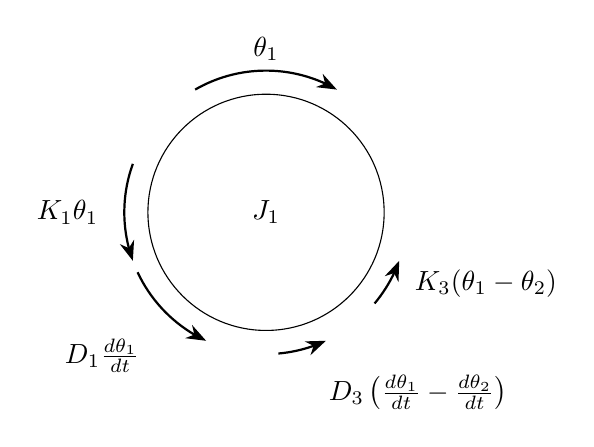
\begin{tikzpicture}[scale=1]
            % Mass J1
            \node[draw, circle, minimum size=3cm] (j1) {$J_1$};
            % Positive direction arrow
            \draw[-{Stealth[length=2.5mm]}, thick] (120:1.8cm) arc (120:60:1.8cm) node[midway, above] {$\theta_1$};
            
            % Torques on the left (from wall) - counter-clockwise
            \draw[{Stealth[length=2.5mm]}-, thick, black] (200:1.8cm) arc(200:160:1.8cm) node[midway, left=2mm]{$K_1\theta_1$};
            \draw[{Stealth[length=2.5mm]}-, thick, black] (245:1.8cm) arc(245:205:1.8cm) node[midway, below left=2mm]{$D_1\frac{d\theta_1}{dt}$};
            
            % Torques on the right (from J2) - counter-clockwise
            \draw[{Stealth[length=2.5mm]}-, thick, black] (340:1.8cm) arc(340:320:1.8cm) node[midway, right=2mm]{$K_3(\theta_1-\theta_2)$};
            \draw[{Stealth[length=2.5mm]}-, thick, black] (295:1.8cm) arc(295:275:1.8cm) node[midway, below right=2mm]{$D_3\left(\frac{d\theta_1}{dt}-\frac{d\theta_2}{dt}\right)$};
            
        \end{tikzpicture}
    \end{minipage}
    \hfill
    \begin{minipage}{0.48\textwidth}
        \centering
        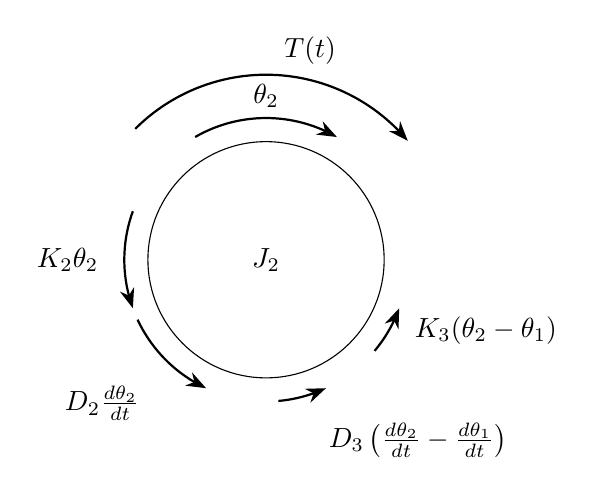
\begin{tikzpicture}[scale=1]
            % Mass J2
            \node[draw, circle, minimum size=3cm] (j2) {$J_2$};
             % Positive direction arrow
            \draw[-{Stealth[length=2.5mm]}, thick] (120:1.8cm) arc (120:60:1.8cm) node[midway, above] {$\theta_2$};
            
            % Applied Torque T(t) - clockwise
            \draw[-{Stealth[length=2.5mm]}, thick, black!50!black] (135:2.35cm) arc (135:40:2.35cm) node[midway, above right] {$T(t)$};
            
            % Torques on the left (from wall) - counter-clockwise
            \draw[{Stealth[length=2.5mm]}-, thick, black] (200:1.8cm) arc(200:160:1.8cm) node[midway, left=2mm]{$K_2\theta_2$};
            \draw[{Stealth[length=2.5mm]}-, thick, black] (245:1.8cm) arc(245:205:1.8cm) node[midway, below left=2mm]{$D_2\frac{d\theta_2}{dt}$};
            
            % Torques on the right (from J1) - counter-clockwise
            \draw[{Stealth[length=2.5mm]}-, thick, black] (340:1.8cm) arc(340:320:1.8cm) node[midway, right=2mm]{$K_{3}(\theta_2-\theta_1)$};
            \draw[{Stealth[length=2.5mm]}-, thick, black] (295:1.8cm) arc(295:275:1.8cm) node[midway, below right=2mm]{$D_3\left(\frac{d\theta_2}{dt}-\frac{d\theta_1}{dt}\right)$};
            
        \end{tikzpicture}
    \end{minipage}
\end{figure}


\noindent\textbf{Equations of Motion}

\vspace{8pt}

\noindent We apply Newton's second law for rotation ($\sum \tau = J \frac{d^2\theta}{dt^2}$) to each mass.

\vspace{8pt}

{For Inertia 1 ($J_1$):}
\begin{align*}
    J_1 \frac{d^2\theta_1}{dt^2} + D_1 \frac{d\theta_1}{dt} + K_1 \theta_1 + D_3\left(\frac{d\theta_1}{dt} - \frac{d\theta_2}{dt}\right) + K_{3}(\theta_1 - \theta_2) &= 0 \\
    J_1 \frac{d^2\theta_1}{dt^2} + (D_1 + D_3)\frac{d\theta_1}{dt} + (K_1 + K_{3})\theta_1 - D_{3}\frac{d\theta_2}{dt} - K_{3}\theta_2 &= 0
\end{align*}

{For Inertia 2 ($J_2$):}
\begin{align*}
    J_2 \frac{d^2\theta_2}{dt^2} + D_2 \frac{d\theta_2}{dt} + K_2 \theta_2 + D_{3}\left(\frac{d\theta_2}{dt} - \frac{d\theta_1}{dt}\right) + K_{3}(\theta_2 - \theta_1) &= T(t) \\
    J_2 \frac{d^2\theta_2}{dt^2} + (D_2 + D_{3})\frac{d\theta_2}{dt} + (K_2 + K_{3})\theta_2 - D_{3}\frac{d\theta_1}{dt} - K_{3}\theta_1 &= T(t)
\end{align*}

\newpage
\noindent\textbf{Laplace Transform}

\vspace{12pt}

We take the Laplace transform of the equations, assuming zero initial conditions.

\vspace{8pt}

Equation for Inertia 1:
\[
[J_1 s^2 + (D_1 + D_{3})s + (K_1 + K_{3})]\Theta_1(s) - [D_{3}s + K_{3}]\Theta_2(s) = 0
\]

Equation for Inertia 2:
\[
-[D_{3}s + K_{3}]\Theta_1(s) + [J_2 s^2 + (D_2 + D_{3})s + (K_2 + K_{3})]\Theta_2(s) = T(s)
\]

Substituting the given numerical values:
\begin{align}
    (s^2 + 5s + 6)\Theta_1(s) - (3s + 4)\Theta_2(s) &= 0 \tag{1} \\
    -(3s + 4)\Theta_1(s) + (s^2 + 5s + 5)\Theta_2(s) &= T(s) \tag{2}
\end{align}

\noindent\textbf{Solving for the Transfer Function}
\vspace{8pt}

From equation (1), we express $\Theta_2(s)$ in terms of $\Theta_1(s)$:
\[
\Theta_2(s) = \frac{s^2 + 5s + 6}{3s + 4} \Theta_1(s)
\]

Substitute this into equation (2):
\[
-(3s + 4)\Theta_1(s) + (s^2 + 5s + 5) \left( \frac{s^2 + 5s + 6}{3s + 4} \Theta_1(s) \right) = T(s)
\]

Factor out $\Theta_1(s)$:
\[
\left[ \frac{-(3s + 4)^2 + (s^2 + 5s + 5)(s^2 + 5s + 6)}{3s + 4} \right] \Theta_1(s) = T(s)
\]

Rearrange to find the transfer function $\dfrac{\Theta_1(s)}{T(s)}$:
\[
\frac{\Theta_1(s)}{T(s)} = \frac{3s + 4}{(s^2 + 5s + 5)(s^2 + 5s + 6) - (3s + 4)^2}
\]

Expand and simplify the denominator:
\begin{align*}
    \text{Denominator} &= (s^4 + 10s^3 + 36s^2 + 55s + 30) - (9s^2 + 24s + 16) \\
    &= s^4 + 10s^3 + (36 - 9)s^2 + (55 - 24)s + (30 - 16) \\
    &= s^4 + 10s^3 + 27s^2 + 31s + 14
\end{align*}

The final transfer function is:
\[
\boxed{\frac{\Theta_1(s)}{T(s)} = \frac{3s + 4}{s^4 + 10s^3 + 27s^2 + 31s + 14}}
\]
% Problem 17 - Rotational Mechanical System Transfer Functions

\newpage
% command for new page 
  \setcounter{page}{32}  
\noindent\rule{\textwidth}{1pt}
\noindent\textbf{Problem 17} \hfill 
%palagay ulit dito 'yung problem statement
\\ For the given system, find the transfer function $\frac{\theta_2(s)}{T(s)}$.

\vspace{-2em}
\begin{figure}[!ht]
\centering
\resizebox{0.9\textwidth}{!}{%
\begin{circuitikz}
\tikzstyle{every node}=[font=\large]


\filldraw[pattern=bricks, pattern color=black!60] (-1.75,13.25) rectangle (-1.25,9.75);
\filldraw[pattern=bricks, pattern color=black!60] (15.25,13.25) rectangle (15.75,9.75);

\draw [short] (-1.25,12) -- (-0.25,12);
\draw [short] (0.5,12.5) -- (-0.25,12.5);
\draw [short] (-0.25,12.5) -- (-0.25,11.5);
\draw [short] (1,12) -- (0.25,12);
\draw [short] (0.5,11.5) -- (-0.25,11.5);
\draw [short] (0.25,12.25) -- (0.25,11.75);
\draw (-1.25,10.75) to[L ] (2.5,10.75);
\draw (1,12) to[L ] (2.5,12);
\draw (2.5,11.5) ellipse (0.25cm and 1cm);
\draw [short] (2.5,10.5) -- (6.25,10.5);
\draw [short] (2.5,12.5) -- (6.25,12.5);
\draw [short] (6.25,12.5) .. controls (6.75,12.25) and (6.5,10.5) .. (6.25,10.5);
\draw [short] (6.5,12) -- (7.5,12);
\draw [short] (8.25,12.5) -- (7.5,12.5);
\draw [short] (7.5,12.5) -- (7.5,11.5);
\draw [short] (9.5,12) -- (8,12);
\draw [short] (8.25,11.5) -- (7.5,11.5);
\draw [short] (8,12.25) -- (8,11.75);
\draw (6.5,10.75) to[L ] (9.5,10.75);
\draw (9.5,11.5) ellipse (0.25cm and 1cm);
\draw [short] (9.5,10.5) -- (13.25,10.5);
\draw [short] (9.5,12.5) -- (13.25,12.5);
\draw [short] (13.25,12.5) .. controls (13.75,12.25) and (13.5,10.5) .. (13.25,10.5);
\draw (13.5,11.5) to[L ] (15.25,11.5);
\node [font=\large] at (0,13.5) {1N-m-s/rad};
\node [font=\large] at (2,13) {1N-m/rad};
\node [font=\large] at (0.5,10) {1N-m/rad};
\node [font=\large] at (11.75,11.5) {$2kg-m^2$};
\node [font=\large] at (4.5,11.5) {$2kg-m^2$};
\node [font=\large] at (8,13) {1N-m-s/rad};
\node [font=\large] at (8,10) {1N-m/rad};
\node [font=\large] at (14.25,12.75) {1N-m/rad};
\draw [ color={rgb,255:red,46; green,128; blue,163}, ->, >=Stealth] (3.75,10.25) .. controls (3,10.5) and (3.25,14.5) .. (3.75,12.5) ;
\draw [ color={rgb,255:red,46; green,128; blue,163}, ->, >=Stealth] (10.5,10.25) .. controls (9.75,10.5) and (10,14.5) .. (10.5,12.5) ;
\draw [ color={rgb,255:red,46; green,128; blue,163}, ->, >=Stealth] (12,10.25) .. controls (11.25,10.5) and (11.5,14.5) .. (12,12.5) ;
\node [font=\large, color={rgb,255:red,46; green,128; blue,163}] at (3.75,13.5) {$\theta_1(t)$};
\node [font=\large, color={rgb,255:red,46; green,128; blue,163}] at (10.25,13.5) {$T(t)$};
\node [font=\large, color={rgb,255:red,46; green,128; blue,163}] at (11.75,13.5) {$\theta_2(t)$};
\end{circuitikz}
}%
\end{figure}


\noindent\rule{\textwidth}{1pt}

\vspace{12pt}

\noindent\textbf{\textit{Given:}}

\begin{center}
    $J_1 = 2\, \text{kg-m}^2$, $J_2 = 2\, \text{kg-m}^2$ \\[6pt]
    $D_1 = 1\, \text{N-m-s/rad}$, $D_2 = 1\, \text{N-m-s/rad}$, $D_3 = 1\, \text{N-m-s/rad}$ \\[6pt]
    $K_1 = 1\, \text{N-m/rad}$, $K_2 = 1\, \text{N-m/rad}$, $K_3 = 1\, \text{N-m/rad}$
\end{center}


\noindent\textbf{\textit{Required:}}
\[
\frac{\theta_2(s)}{F(s)}
\]


\vspace{1.5em}
\noindent\textbf{\textit{Solution:}}

\vspace{8pt}

\noindent\textbf{Free-Body Diagrams (FBDs)}
\vspace{12pt}

We assume clockwise rotation is positive.

\begin{figure}[h!]
    \centering
    \begin{minipage}{0.48\textwidth}
        \centering
        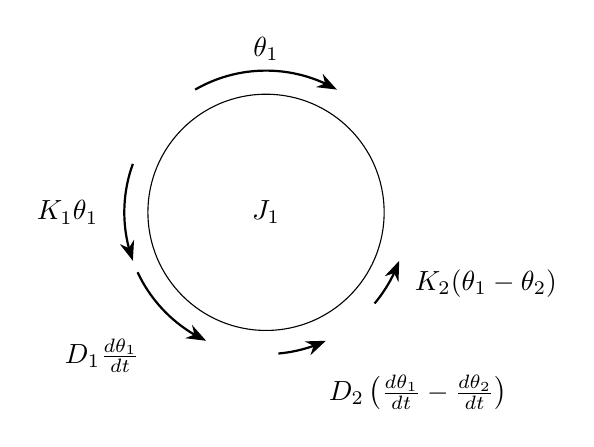
\begin{tikzpicture}[scale=1]
            % J1
            \node[draw, circle, minimum size=3cm] (j1) {$J_1$};
            \draw[-{Stealth[length=2.5mm]}, thick] (120:1.8cm) arc (120:60:1.8cm) node[midway, above] {$\theta_1$};
            % Wall Torques (CCW)
            \draw[{Stealth[length=2.5mm]}-, thick] (200:1.8cm) arc(200:160:1.8cm) node[midway, left=2mm]{$K_1\theta_1$};
            \draw[{Stealth[length=2.5mm]}-, thick] (245:1.8cm) arc(245:205:1.8cm) node[midway, below left=2mm]{$D_1\frac{d\theta_1}{dt}$};
            % Connecting Torques (CCW)
            \draw[{Stealth[length=2.5mm]}-, thick] (340:1.8cm) arc(340:320:1.8cm) node[midway, right=2mm]{$K_2(\theta_1-\theta_2)$};
            \draw[{Stealth[length=2.5mm]}-, thick] (295:1.8cm) arc(295:275:1.8cm) node[midway, below right=2mm]{$D_2\left(\frac{d\theta_1}{dt}-\frac{d\theta_2}{dt}\right)$};
        \end{tikzpicture}
    \end{minipage}
    \hfill
    \begin{minipage}{0.48\textwidth}
        \centering
        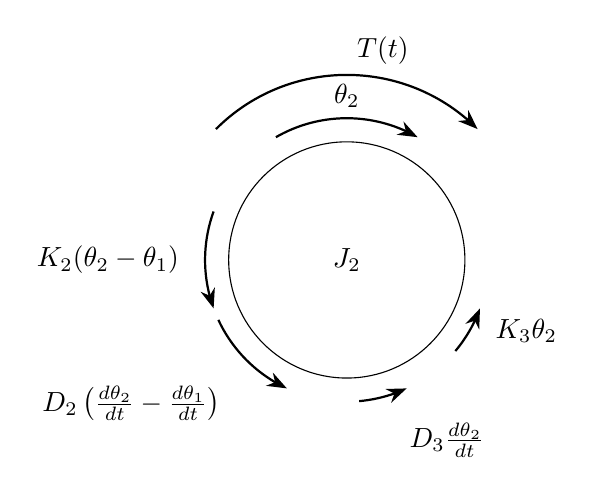
\begin{tikzpicture}[scale=1]
            % J2
            \node[draw, circle, minimum size=3cm] (j2) {$J_2$};
            \draw[-{Stealth[length=2.5mm]}, thick] (120:1.8cm) arc (120:60:1.8cm) node[midway, above] {$\theta_2$};
            % Applied Torque T(t) (CW)
            \draw[-{Stealth[length=2.5mm]}, thick] (135:2.35cm) arc (135:45:2.35cm) node[midway, above right] {$T(t)$};
            % Wall Torques (CCW)
            \draw[{Stealth[length=2.5mm]}-, thick] (340:1.8cm) arc(340:320:1.8cm) node[midway, right=2mm]{$K_3\theta_2$};
            \draw[{Stealth[length=2.5mm]}-, thick] (295:1.8cm) arc(295:275:1.8cm) node[midway, below right=2mm]{$D_3\frac{d\theta_2}{dt}$};
            % Connecting Torques (CCW)
            \draw[{Stealth[length=2.5mm]}-, thick] (200:1.8cm) arc(200:160:1.8cm) node[midway, left=2mm]{$K_2(\theta_2-\theta_1)$};
            \draw[{Stealth[length=2.5mm]}-, thick] (245:1.8cm) arc(245:205:1.8cm) node[midway, below left=2mm]{$D_2\left(\frac{d\theta_2}{dt}-\frac{d\theta_1}{dt}\right)$};
        \end{tikzpicture}
    \end{minipage}
\end{figure}

\noindent\textbf{Equations of Motion}
\vspace{8pt}

\noindent We apply Newton's second law for rotation ($\sum \tau = J \frac{d^2\theta}{dt^2}$) to each inertia.

\vspace{5pt}
{For Inertia 1 ($J_1$):}
\begin{align*}
    J_1 \frac{d^2\theta_1}{dt^2} + D_1 \frac{d\theta_1}{dt} + K_1 \theta_1 + D_2\left(\frac{d\theta_1}{dt} - \frac{d\theta_2}{dt}\right) + K_2(\theta_1 - \theta_2) &= 0 \\
    J_1 \frac{d^2\theta_1}{dt^2} + (D_1 + D_2)\frac{d\theta_1}{dt} + (K_1 + K_2)\theta_1 - D_2\frac{d\theta_2}{dt} - K_2\theta_2 &= 0
\end{align*}

{For Inertia 2 ($J_2$):}
\begin{align*}
    J_2 \frac{d^2\theta_2}{dt^2} + D_3 \frac{d\theta_2}{dt} + K_3 \theta_2 + D_2\left(\frac{d\theta_2}{dt} - \frac{d\theta_1}{dt}\right) + K_2(\theta_2 - \theta_1) &= T(t) \\
    J_2 \frac{d^2\theta_2}{dt^2} + (D_2 + D_3)\frac{d\theta_2}{dt} + (K_2 + K_3)\theta_2 - D_2\frac{d\theta_1}{dt} - K_2\theta_1 &= T(t)
\end{align*}

\newpage
\noindent\textbf{Laplace Transform}
\vspace{12pt}

We take the Laplace transform of the equations, assuming zero initial conditions.

Equation for Inertia 1:
\[
[J_1 s^2 + (D_1 + D_2)s + (K_1 + K_2)]\Theta_1(s) - [D_2s + K_2]\Theta_2(s) = 0
\]

Equation for Inertia 2:
\[
-[D_2s + K_2]\Theta_1(s) + [J_2 s^2 + (D_2 + D_3)s + (K_2 + K_3)]\Theta_2(s) = T(s)
\]

Substituting the numerical values:
\begin{align}
    (2s^2 + 2s + 4)\Theta_1(s) - (s + 2)\Theta_2(s) &= 0 \tag{1} \\
    -(s + 2)\Theta_1(s) + (2s^2 + 2s + 3)\Theta_2(s) &= T(s) \tag{2}
\end{align}

\noindent\textbf{Solving for the Transfer Function}
\vspace{8pt}

From equation (1), we express $\Theta_1(s)$ in terms of $\Theta_2(s)$:
\[
\Theta_1(s) = \frac{s + 2}{2s^2 + 2s + 4} \Theta_2(s)
\]

Substitute this into equation (2):
\[
-(s + 2) \left( \frac{s + 2}{2s^2 + 2s + 4} \Theta_2(s) \right) + (2s^2 + 2s + 3) \Theta_2(s) = T(s)
\]

Factor out $\Theta_2(s)$:
\[
\left[ \frac{-(s + 2)^2 + (2s^2 + 2s + 3)(2s^2 + 2s + 4)}{2s^2 + 2s + 4} \right] \Theta_2(s) = T(s)
\]

Rearrange to find the transfer function $\dfrac{\Theta_2(s)}{T(s)}$:
\[
\frac{\Theta_2(s)}{T(s)} = \frac{2s^2 + 2s + 4}{(2s^2 + 2s + 3)(2s^2 + 2s + 4) - (s + 2)^2}
\]

Expand and simplify the denominator:
\begin{align*}
    \text{Denominator} &= (4s^4 + 8s^3 + 14s^2 + 14s + 12) - (s^2 + 4s + 4) \\
    &= 4s^4 + 8s^3 + (14 - 1)s^2 + (14 - 4)s + (12 - 4) \\
    &= 4s^4 + 8s^3 + 13s^2 + 10s + 8
\end{align*}

The final transfer function is:
\[
\boxed{\frac{\Theta_2(s)}{T(s)} = \frac{2s^2 + 2s + 4}{4s^4 + 8s^3 + 13s^2 + 10s + 8}}
\]


% Problem 18 - Rotational Mechanical System Transfer Functions
\newpage
% command for new page 
  \setcounter{page}{34}  
\noindent\rule{\textwidth}{1pt}
\noindent\textbf{Problem 18} \hfill 
%palagay ulit dito 'yung problem statement
\\ For the given system, find the transfer function $\frac{\theta_1(s)}{T(s)}$.

\begin{figure}[!ht]
\centering
\resizebox{0.8\textwidth}{!}{%
\begin{circuitikz}
\tikzstyle{every node}=[font=\normalsize]


\filldraw [pattern=bricks, pattern color=black!60] (-0.25,40) rectangle (0.5,36.25);
\filldraw [pattern=bricks, pattern color=black!60] (14.75,40) rectangle (15.5,36.25);

\draw (4.5,38) ellipse (0.25cm and 0.75cm);
\draw [short] (4.5,38.75) -- (7.25,38.75);
\draw [short] (4.5,37.25) -- (7.25,37.25);
\draw (9.5,38) ellipse (0.25cm and 0.75cm);
\draw [short] (9.5,38.75) -- (12.25,38.75);
\draw [short] (9.5,37.25) -- (12.25,37.25);
\draw (7.5,38.5) to [short] (8,38.5);
\draw (8,38.5) to [short] (8,39);
\draw (8,39) to [short] (9,39);
\draw (8,38.5) to [short] (8,38);
\draw (8,38) to [short] (9,38);
\draw (8.5,38.75) to [short] (8.5,38.25);
\draw (8.5,38.5) to [short] (9.5,38.5);
\draw (7.5,37.5) to [L ] (9.5,37.5);
\node [font=\normalsize] at (11,38) {$ 2 kg-m^2$};
\node [font=\normalsize] at (6,38) {$ 1 kg-m^2$};
\node [font=\normalsize] at (8.5,39.25) {$1 N-m-s/rad$};
\node [font=\normalsize] at (8.25,37) {$1 N-m/rad$};
\draw [color={rgb,255:red,46; green,128; blue,163}, ->, >=Stealth] (6,36.75) .. controls (5.25,37.5) and (5.75,40.5) .. (6.25,38.75) ;
\draw [color={rgb,255:red,46; green,128; blue,163}, ->, >=Stealth] (5.25,36.75) .. controls (4.5,37.5) and (5,40.5) .. (5.5,38.75) ;
\draw [color={rgb,255:red,46; green,128; blue,163}, ->, >=Stealth] (11.5,36.75) .. controls (10.75,37.5) and (11.25,40.5) .. (11.75,38.75) ;
\node [font=\normalsize, color={rgb,255:red,46; green,128; blue,163}] at (6,39.75) {$\theta_1(t)$};
\node [font=\normalsize, color={rgb,255:red,46; green,128; blue,163}] at (5,39.75) {\textit{T(t)}};
\node [font=\normalsize, color={rgb,255:red,46; green,128; blue,163}] at (11.5,39.75) {$\theta_2(t)$};
\draw [short] (7.25,38.75) .. controls (7.75,38.5) and (7.5,37.25) .. (7.25,37.25);
\draw [short] (12.25,38.75) .. controls (12.75,38.5) and (12.5,37.25) .. (12.25,37.25);
\draw (0.5,38) to [short] (1,38);
\draw (1,38) to [short] (1,38.5);
\draw (1,38.5) to [short] (2,38.5);
\draw (1,38) to [short] (1,37.5);
\draw (1,37.5) to [short] (2,37.5);
\draw (1.5,38.25) to [short] (1.5,37.75);
\draw (1.5,38) to [short] (2.5,38);
\node [font=\normalsize] at (2,38.75) {$1 N-m-s/rad$};
\node [font=\normalsize] at (3.2,37.25) {$1 N-m/rad$};
\draw (2.5,38) to [L ] (4.5,38);
\draw (12.5,38.5) to [short] (13,38.5);
\draw (13,38.5) to [short] (13,39);
\draw (13,39) to [short] (14,39);
\draw (13,38.5) to [short] (13,38);
\draw (13,38) to [short] (14,38);
\draw (13.5,38.75) to [short] (13.5,38.25);
\draw (13.5,38.5) to [short] (14.75,38.5);
\node [font=\normalsize] at (13.3,39.25) {$1 N-m-s/rad$};
\node [font=\normalsize] at (13.30,37) {$1 N-m/rad$};
\draw (12.5,37.5) to [L ] (14.78,37.5);
\end{circuitikz}
}%
\end{figure}

\noindent\rule{\textwidth}{1pt}

\vspace{12pt}


\noindent\textbf{\textit{Given:}}
\[
J_1 = 1\, \text{kg}\cdot\text{m}^2, \quad J_2 = 2\, \text{kg}\cdot\text{m}^2
\]
\[
D_1,D_2,D_3 = 1\, \text{N}\cdot\text{m}\cdot\text{s/rad}, 
\]
\[
K_1,K_2,K_3 = 1\, \text{N}\cdot\text{m/rad} 
\]

\vspace{1em}
\noindent

\noindent\textbf{\textit{Required:}}
\[
\frac{\theta_1(s)}{F(s)}
\]

\vspace{1.5em}
\noindent\textbf{\textit{Solution:}}

\vspace{8pt}

\noindent\textbf{Free-Body Diagrams (FBDs)}
\vspace{5pt}

\noindent We draw the FBD for each mass. The input torque $T(t)$ is applied to mass $J_1$. Clockwise rotation ($\theta$) is considered positive.

\begin{figure}[h!]
    \centering
    \begin{minipage}{0.48\textwidth}
        \centering
        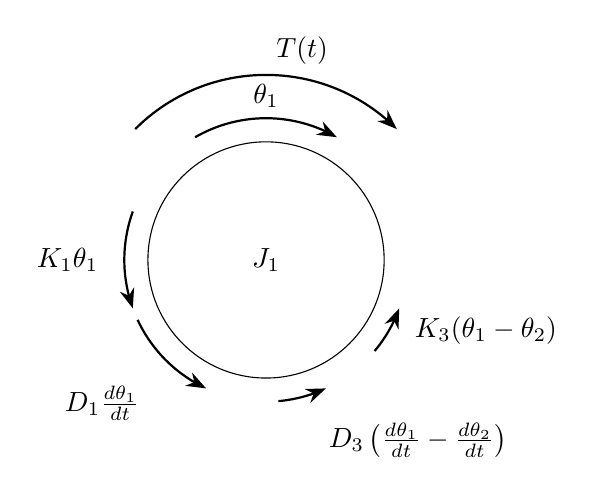
\begin{tikzpicture}[scale=1]
            % Mass J1
            \node[draw, circle, minimum size=3cm] (j1) {$J_1$};
            % Positive direction arrow
            \draw[-{Stealth[length=2.5mm]}, thick] (120:1.8cm) arc (120:60:1.8cm) node[midway, above] {$\theta_1$};
            % Applied Torque T(t) - clockwise
            \draw[-{Stealth[length=2.5mm]}, thick, black!50!black] (135:2.35cm) arc (135:45:2.35cm) node[midway, above right] {$T(t)$};
            % Torques on the left (from wall) - counter-clockwise
            \draw[{Stealth[length=2.5mm]}-, thick, black] (200:1.8cm) arc(200:160:1.8cm) node[midway, left=2mm]{$K_1\theta_1$};
            \draw[{Stealth[length=2.5mm]}-, thick, black] (245:1.8cm) arc(245:205:1.8cm) node[midway, below left=2mm]{$D_1\frac{d\theta_1}{dt}$};
            % Torques on the right (from J2) - counter-clockwise
            \draw[{Stealth[length=2.5mm]}-, thick, black] (340:1.8cm) arc(340:320:1.8cm) node[midway, right=2mm]{$K_3(\theta_1-\theta_2)$};
            \draw[{Stealth[length=2.5mm]}-, thick, black] (295:1.8cm) arc(295:275:1.8cm) node[midway, below right=2mm]{$D_3\left(\frac{d\theta_1}{dt}-\frac{d\theta_2}{dt}\right)$};
        \end{tikzpicture}
    \end{minipage}
    \hfill
    \begin{minipage}{0.48\textwidth}
        \centering
        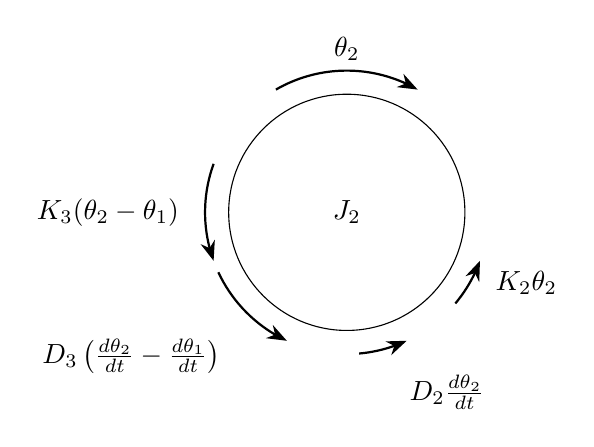
\begin{tikzpicture}[scale=1]
            % Mass J2
            \node[draw, circle, minimum size=3cm] (j2) {$J_2$};
            % Positive direction arrow
            \draw[-{Stealth[length=2.5mm]}, thick] (120:1.8cm) arc (120:60:1.8cm) node[midway, above] {$\theta_2$};
            % Torques on the left (from J1) - counter-clockwise
            \draw[{Stealth[length=2.5mm]}-, thick, black] (200:1.8cm) arc(200:160:1.8cm) node[midway, left=2mm]{$K_3(\theta_2-\theta_1)$};
            \draw[{Stealth[length=2.5mm]}-, thick, black] (245:1.8cm) arc(245:205:1.8cm) node[midway, below left=2mm]{$D_3\left(\frac{d\theta_2}{dt}-\frac{d\theta_1}{dt}\right)$};
            % Torques on the right (from wall) - counter-clockwise
            \draw[{Stealth[length=2.5mm]}-, thick, black] (340:1.8cm) arc(340:320:1.8cm) node[midway, right=2mm]{$K_2\theta_2$};
            \draw[{Stealth[length=2.5mm]}-, thick, black] (295:1.8cm) arc(295:275:1.8cm) node[midway, below right=2mm]{$D_2\frac{d\theta_2}{dt}$};
        \end{tikzpicture}
    \end{minipage}
\end{figure}

\noindent\textbf{Equations of Motion}
\vspace{5pt}

\noindent From the FBDs, we apply Newton's second law for rotation ($\sum \tau = J \frac{d^2\theta}{dt^2}$) to each mass.

\vspace{12pt}
{For Inertia 1 ($J_1$):}
\begin{align*}
% torque balance from FBD
J_1\frac{d^2\theta_1}{dt^2}
+ D_1\frac{d\theta_1}{dt}
+ D_3\!\left(\frac{d\theta_1}{dt}-\frac{d\theta_2}{dt}\right)
+ K_1\theta_1
+ K_3\!\left(\theta_1-\theta_2\right)
- T(t) &= 0 \\[4pt]
% collect terms
J_1\frac{d^2\theta_1}{dt^2}
+ (D_1 + D_3)\frac{d\theta_1}{dt}
+ (K_1 + K_3)\theta_1
- D_3\frac{d\theta_2}{dt}
- K_3\theta_2
- T(t) &= 0 \\[4pt]
J_1\frac{d^2\theta_1}{dt^2}
+ (D_1 + D_3)\frac{d\theta_1}{dt}
+ (K_1 + K_3)\theta_1
- D_3\frac{d\theta_2}{dt}
- K_3\theta_2
&= T(t)
\end{align*}

\newpage
{For Inertia 2 ($J_2$):}
\begin{align*}
% torque balance from FBD
J_2\frac{d^2\theta_2}{dt^2}
+ D_2\frac{d\theta_2}{dt}
+ D_3\!\left(\frac{d\theta_2}{dt}-\frac{d\theta_1}{dt}\right)
+ K_2\theta_2
+ K_3\!\left(\theta_2-\theta_1\right) &= 0 \\[4pt]
% collect terms
J_2\frac{d^2\theta_2}{dt^2}
+ (D_2 + D_3)\frac{d\theta_2}{dt}
- D_3\frac{d\theta_1}{dt}
+ (K_2 + K_3)\theta_2
- K_3\theta_1 &= 0
\end{align*}

\noindent\textbf{Laplace Transform}
\vspace{5pt}

\noindent We take the Laplace transform of the equations, assuming zero initial conditions, and substitute the component values.
\vspace{12pt}

{Substituting values into the transformed equations gives:}
\begin{align}
    (s^2 + 2s + 2)\Theta_1(s) - (s + 1)\Theta_2(s) &= T(s) \tag{1} \\
    -(s + 1)\Theta_1(s) + (2s^2 + 2s + 2)\Theta_2(s) &= 0 \tag{2}
\end{align}

\noindent\textbf{Solving for the Transfer Function}
\vspace{12pt}

\noindent To find $\dfrac{\Theta_1(s)}{T(s)}$, we must eliminate $\Theta_2(s)$. From equation (2), we can express $\Theta_2(s)$ in terms of $\Theta_1(s)$:
\[
\Theta_2(s) = \frac{s + 1}{2s^2 + 2s + 2} \Theta_1(s)
\]

Now, substitute this into equation (1):
\[
(s^2 + 2s + 2)\Theta_1(s) - (s + 1) \left( \frac{s + 1}{2s^2 + 2s + 2} \Theta_1(s) \right) = T(s)
\]

Factor out $\Theta_1(s)$:
\[
\left[ \frac{(s^2 + 2s + 2)(2s^2 + 2s + 2) - (s + 1)^2}{2s^2 + 2s + 2} \right] \Theta_1(s) = T(s)
\]

Rearrange to find the transfer function $\dfrac{\Theta_1(s)}{T(s)}$:
\[
\frac{\Theta_1(s)}{T(s)} = \frac{2s^2 + 2s + 2}{(s^2 + 2s + 2)(2s^2 + 2s + 2) - (s + 1)^2}
\]

Finally, we expand and simplify the denominator:
\begin{align*}
    \text{Term 1: } & (s^2 + 2s + 2)(2s^2 + 2s + 2) = 2s^4 + 6s^3 + 10s^2 + 8s + 4 \\
    \text{Term 2: } & (s + 1)^2 = s^2 + 2s + 1
\end{align*}

Subtracting the two terms gives the final denominator:
\begin{align*}
&= (2s^4 + 6s^3 + 10s^2 + 8s + 4) - (s^2 + 2s + 1) \\
&= 2s^4 + 6s^3 + 9s^2 + 6s + 3
\end{align*}

The final transfer function is:
\[
\boxed{\frac{\Theta_1(s)}{T(s)} = \frac{2s^2 + 2s + 2}{2s^4 + 6s^3 + 9s^2 + 6s + 3}}
\]




% Problem 19 - Rotational Mechanical System Transfer Functions
\newpage
% command for new page 
  \setcounter{page}{36}  
\noindent\rule{\textwidth}{1pt}
\noindent\textbf{Problem 19} \hfill 
%palagay ulit dito 'yung problem statement
\\ For the given system, find the transfer function $\frac{\theta_2(s)}{T(s)}$.

\vspace{-2em}
\begin{figure}[!ht]
\centering
\resizebox{0.9\textwidth}{!}{%
\begin{circuitikz}
\tikzstyle{every node}=[font=\large]

\filldraw[pattern=bricks, pattern color=black!60] (-1.75,13.25) rectangle (-1.25,9.75);
\filldraw[pattern=bricks, pattern color=black!60] (17.75,13.25) rectangle (18.25,9.75);

\draw [short] (0.25,12) -- (1.25,12);
\draw [short] (2,12.5) -- (1.25,12.5);
\draw [short] (1.25,12.5) -- (1.25,11.5);
\draw [short] (2.5,12) -- (1.75,12);
\draw [short] (2,11.5) -- (1.25,11.5);
\draw [short] (1.75,12.25) -- (1.75,11.75);
\draw (-1.25,10.75) to[L ] (2.5,10.75);
\draw (-1.25,12) to[L ] (0.25,12);
\draw (2.5,11.5) ellipse (0.25cm and 1cm);
\draw [short] (2.5,10.5) -- (6.25,10.5);
\draw [short] (2.5,12.5) -- (6.25,12.5);
\draw [short] (6.25,12.5) .. controls (6.75,12.25) and (6.5,10.5) .. (6.25,10.5);
\draw (6.5,11.5) to[L ] (9.5,11.5);
\draw (9.5,11.5) ellipse (0.25cm and 1cm);
\draw [short] (9.5,10.5) -- (13.25,10.5);
\draw [short] (9.5,12.5) -- (13.25,12.5);
\draw [short] (13.25,12.5) .. controls (13.75,12.25) and (13.5,10.5) .. (13.25,10.5);
\node [font=\large] at (2,13) {1N-m-s/rad};
\node [font=\large] at (-0.25,12.75) {2N-m/rad};
\node [font=\large] at (0.5,10) {1N-m/rad};
\node [font=\large] at (11.75,11.5) {$2kg-m^2$};
\node [font=\large] at (4.5,11.5) {$1kg-m^2$};
\node [font=\large] at (8,10.75) {1N-m/rad};
\draw [ color={rgb,255:red,46; green,128; blue,163}, ->, >=Stealth] (3.75,10.25) .. controls (3,10.5) and (3.25,14.5) .. (3.75,12.5) ;
\draw [ color={rgb,255:red,46; green,128; blue,163}, ->, >=Stealth] (10.5,10.25) .. controls (9.75,10.5) and (10,14.5) .. (10.5,12.5) ;
\draw [ color={rgb,255:red,46; green,128; blue,163}, ->, >=Stealth] (12,10.25) .. controls (11.25,10.5) and (11.5,14.5) .. (12,12.5) ;
\node [font=\large, color={rgb,255:red,46; green,128; blue,163}] at (3.75,13.5) {$\theta_1(t)$};
\node [font=\large, color={rgb,255:red,46; green,128; blue,163}] at (10.25,13.5) {$T(t)$};
\node [font=\large, color={rgb,255:red,46; green,128; blue,163}] at (11.75,13.5) {$\theta_2(t)$};
\draw [short] (13.5,12) -- (14.5,12);
\draw [short] (15.25,12.5) -- (14.5,12.5);
\draw [short] (14.5,12.5) -- (14.5,11.5);
\draw [short] (15.75,12) -- (15,12);
\draw [short] (15.25,11.5) -- (14.5,11.5);
\draw [short] (15,12.25) -- (15,11.75);
\draw (15.75,12) to[L ] (17.75,12);
\node [font=\large] at (14.5,12.75) {2N-m-s/rad};
\node [font=\large] at (16.75,13) {1N-m/rad};
\node [font=\large] at (15.25,10) {1N-m/rad};
\draw (13.5,10.75) to[L ] (17.75,10.75);
\end{circuitikz}
}%
\end{figure}

\noindent\rule{\textwidth}{1pt}

\vspace{12pt}


\noindent\textbf{\textit{Given:}}
\[
J_1 = 1\, \text{kg}\cdot\text{m}^2, \quad J_2 = 2\, \text{kg}\cdot\text{m}^2
\]
\[
D_1 = 1\, \text{N}\cdot\text{m}\cdot\text{s/rad}, \quad D_2 = 2\, \text{N}\cdot\text{m}\cdot\text{s/rad}
\]
\[
K_1 = 2\, \text{N}\cdot\text{m/rad}, \quad K_2,K_3K_4 = 1\, \text{N}\cdot\text{m/rad}
\]


\vspace{1em}
\noindent

\noindent\textbf{\textit{Required:}}
\[
\frac{\theta_2(s)}{F(s)}
\]

\vspace{1.5em}
\noindent\textbf{\textit{Solution:}}

\vspace{8pt}

\noindent\textbf{Free-Body Diagrams (FBDs)}
\vspace{12pt}

We assume clockwise rotation is positive. The torques shown are the reaction torques opposing positive motion.

\begin{figure}[h!]
    \centering
    \begin{minipage}{0.48\textwidth}
        \centering
        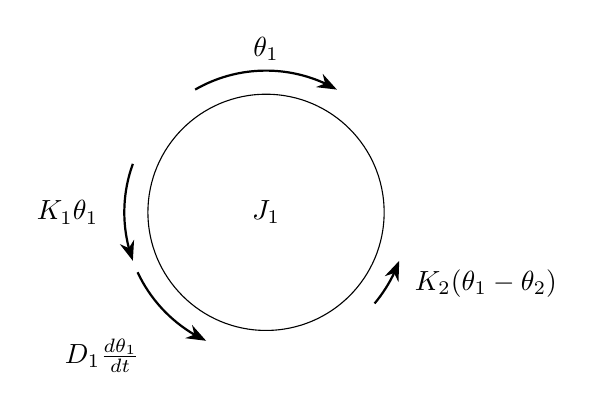
\begin{tikzpicture}[scale=1]
            % J1
            \node[draw, circle, minimum size=3cm] (j1) {$J_1$};
            \draw[-{Stealth[length=2.5mm]}, thick] (120:1.8cm) arc (120:60:1.8cm) node[midway, above] {$\theta_1$};
            % Wall Torques (CCW)
            \draw[{Stealth[length=2.5mm]}-, thick] (200:1.8cm) arc(200:160:1.8cm) node[midway, left=2mm]{$K_1\theta_1$};
            \draw[{Stealth[length=2.5mm]}-, thick] (245:1.8cm) arc(245:205:1.8cm) node[midway, below left=2mm]{$D_1\frac{d\theta_1}{dt}$};
            % Connecting Torques (CCW)
            \draw[{Stealth[length=2.5mm]}-, thick] (340:1.8cm) arc(340:320:1.8cm) node[midway, right=2mm]{$K_2(\theta_1-\theta_2)$};
        \end{tikzpicture}
    \end{minipage}
    \hfill
    \begin{minipage}{0.48\textwidth}
        \centering
        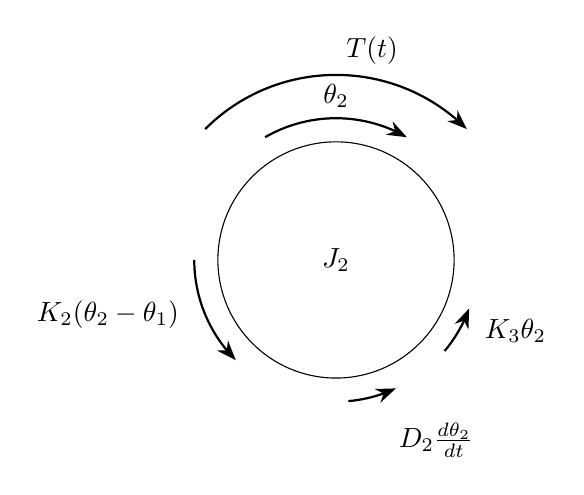
\begin{tikzpicture}[scale=1]
            % J2
            \node[draw, circle, minimum size=3cm] (j2) {$J_2$};
            \draw[-{Stealth[length=2.5mm]}, thick] (120:1.8cm) arc (120:60:1.8cm) node[midway, above] {$\theta_2$};
            % Applied Torque T(t) (CW)
            \draw[-{Stealth[length=2.5mm]}, thick] (135:2.35cm) arc (135:45:2.35cm) node[midway, above right] {$T(t)$};
            % Wall Torques (CCW)
            \draw[{Stealth[length=2.5mm]}-, thick] (340:1.8cm) arc(340:320:1.8cm) node[midway, right=2mm]{$K_3\theta_2$};
            \draw[{Stealth[length=2.5mm]}-, thick] (295:1.8cm) arc(295:275:1.8cm) node[midway, below right=2mm]{$D_2\frac{d\theta_2}{dt}$};
            % Connecting Torques (CCW)
            \draw[{Stealth[length=2.5mm]}-, thick] (225:1.8cm) arc(225:180:1.8cm) node[midway, left=2mm]{$K_2(\theta_2-\theta_1)$};
        \end{tikzpicture}
    \end{minipage}
\end{figure}

\noindent\textbf{Equations of Motion}
\vspace{8pt}

\noindent We apply Newton's second law for rotation ($\sum \tau = J \frac{d^2\theta}{dt^2}$) to each inertia.

\vspace{5pt}
{For Inertia 1 ($J_1$):}
\begin{align*}
    J_1 \frac{d^2\theta_1}{dt^2} + D_1 \frac{d\theta_1}{dt} + K_1 \theta_1 + K_2(\theta_1 - \theta_2) &= 0 \\
    J_1 \frac{d^2\theta_1}{dt^2} + D_1\frac{d\theta_1}{dt} + (K_1 + K_2)\theta_1 - K_2\theta_2 &= 0
\end{align*}

{For Inertia 2 ($J_2$):}
\begin{align*}
    J_2 \frac{d^2\theta_2}{dt^2} + D_2 \frac{d\theta_2}{dt} + K_3 \theta_2 + K_2(\theta_2 - \theta_1) &= T(t) \\
    J_2 \frac{d^2\theta_2}{dt^2} + D_2\frac{d\theta_2}{dt} + (K_2 + K_3)\theta_2 - K_2\theta_1 &= T(t)
\end{align*}

\newpage
\noindent\textbf{Laplace Transform}
\vspace{12pt}

We take the Laplace transform of the equations, assuming zero initial conditions.

Equation for Inertia 1:
\[
[J_1 s^2 + D_1s + (K_1 + K_2)]\Theta_1(s) - K_2\Theta_2(s) = 0
\]

Equation for Inertia 2:
\[
-K_2\Theta_1(s) + [J_2 s^2 + D_2s + (K_2 + K_3)]\Theta_2(s) = T(s)
\]

Substituting the corrected numerical values:
\begin{align}
    (s^2 + s + 4)\Theta_1(s) - \Theta_2(s) &= 0 \tag{1} \\
    -\Theta_1(s) + (2s^2 + 2s + 3)\Theta_2(s) &= T(s) \tag{2}
\end{align}

\noindent\textbf{Solving for the Transfer Function}
\vspace{8pt}

The required transfer function is $G(s) = \dfrac{\Theta_2(s)}{T(s)}$. From equation (1), we express $\Theta_1(s)$ in terms 

of $\Theta_2(s)$:
\[
\Theta_1(s) = \frac{1}{s^2 + s + 4} \Theta_2(s)
\]

Substitute this into equation (2):
\[
- \left( \frac{1}{s^2 + s + 4} \Theta_2(s) \right) + (2s^2 + 2s + 3) \Theta_2(s) = T(s)
\]

Factor out $\Theta_2(s)$:
\[
\left[ \frac{-1 + (2s^2 + 2s + 3)(s^2 + s + 4)}{s^2 + s + 4} \right] \Theta_2(s) = T(s)
\]

Rearrange to find the transfer function $\dfrac{\Theta_2(s)}{T(s)}$:
\[
\frac{\Theta_2(s)}{T(s)} = \frac{s^2 + s + 4}{(2s^2 + 2s + 3)(s^2 + s + 4) - 1}
\]

Expand and simplify the denominator:
\begin{align*}
    \text{Denominator} &= (2s^4 + 2s^3 + 8s^2 + 2s^3 + 2s^2 + 8s + 3s^2 + 3s + 12) - 1 \\
    &= 2s^4 + 4s^3 + 13s^2 + 11s + 11
\end{align*}

The final, corrected transfer function is:
\[
\boxed{\frac{\Theta_2(s)}{T(s)} = \frac{s^2 + s + 4}{2s^4 + 4s^3 + 13s^2 + 11s + 11}}
\]
% Problem 20 - Rotational Mechanical System Transfer Functions
\newpage
% command for new page 
  \setcounter{page}{38}  
\noindent\rule{\textwidth}{1pt}
\noindent\textbf{Problem 20} \hfill 
%palagay ulit dito 'yung problem statement
\\ For the given system, find the transfer function $\frac{\theta_2(s)}{T(s)}$.

\begin{figure}[!ht]
\centering
\resizebox{1\textwidth}{!}{%
\begin{circuitikz}
\tikzstyle{every node}=[font=\normalsize]

\filldraw[pattern=bricks, pattern color=black!60] (-0.25,39.25) rectangle (0.5,35.5);
\filldraw[pattern=bricks, pattern color=black!60] (16.5,39.25) rectangle (17.25,35.5);

\draw (4.5,37.25) ellipse (0.25cm and 0.75cm);
\draw [short] (4.5,38) -- (7.25,38);
\draw [short] (4.5,36.5) -- (7.25,36.5);
\draw (9.5,37.25) ellipse (0.25cm and 0.75cm);
\draw [short] (9.5,38) -- (12.25,38);
\draw [short] (9.5,36.5) -- (12.25,36.5);
\draw (7.5,37.75) to[short] (8,37.75);
\draw (8,37.75) to[short] (8,38.25);
\draw (8,38.25) to[short] (9,38.25);
\draw (8,37.75) to[short] (8,37.25);
\draw (8,37.25) to[short] (9,37.25);
\draw (8.5,38) to[short] (8.5,37.5);
\draw (8.5,37.75) to[short] (9.5,37.75);
\draw (7.5,36.75) to[L ] (9.5,36.75);
\node [font=\normalsize] at (11,37.25) {$ 2 kg-m^2$};
\node [font=\normalsize] at (6,37.25) {$ 4 kg-m^2$};
\node [font=\normalsize] at (8.5,38.5) {$1 N-m-s/rad$};
\node [font=\normalsize] at (8.25,36.25) {$1 N-m/rad$};
\draw [ color={rgb,255:red,46; green,128; blue,163}, ->, >=Stealth] (6,36) .. controls (5.25,36.75) and (5.75,39.75) .. (6.25,38) ;
\draw [ color={rgb,255:red,46; green,128; blue,163}, ->, >=Stealth] (5.25,36) .. controls (4.5,36.75) and (5,39.75) .. (5.5,38) ;
\draw [ color={rgb,255:red,46; green,128; blue,163}, ->, >=Stealth] (11.5,36) .. controls (10.75,36.75) and (11.25,39.75) .. (11.75,38) ;
\node [font=\normalsize, color={rgb,255:red,46; green,128; blue,163}] at (6,39) {$\theta_1(t)$};
\node [font=\normalsize, color={rgb,255:red,46; green,128; blue,163}] at (5,39) {\textit{T(t)}};
\node [font=\normalsize, color={rgb,255:red,46; green,128; blue,163}] at (11.5,39) {$\theta_2(t)$};
\draw [short] (7.25,38) .. controls (7.75,37.75) and (7.5,36.5) .. (7.25,36.5);
\draw [short] (12.25,38) .. controls (12.75,37.75) and (12.5,36.5) .. (12.25,36.5);
\draw (12.5,37.25) to[short] (13,37.25);
\draw (13,37.25) to[short] (13,37.75);
\draw (13,37.75) to[short] (14,37.75);
\draw (13,37.25) to[short] (13,36.75);
\draw (13,36.75) to[short] (14,36.75);
\draw (13.5,37.5) to[short] (13.5,37);
\draw (13.5,37.25) to[short] (14.5,37.25);
\node [font=\normalsize] at (13.8,38) {$2 N-m-s/rad$};
\node [font=\normalsize] at (15.3,36.5) {$1 N-m/rad$};
\draw (14.5,37.25) to[L ] (16.5,37.25);
\draw (0.5,37.25) to[short] (1,37.25);
\draw (1,37.25) to[short] (1,37.75);
\draw (1,37.75) to[short] (2,37.75);
\draw (1,37.25) to[short] (1,36.75);
\draw (1,36.75) to[short] (2,36.75);
\draw (1.5,37.5) to[short] (1.5,37);
\draw (1.5,37.25) to[short] (2.5,37.25);
\node [font=\normalsize] at (2,38) {$2 N-m-s/rad$};
\node [font=\normalsize] at (3.1,36.5) {$1 N-m/rad$};
\draw (2.5,37.25) to[L ] (4.5,37.25);
\end{circuitikz}
}%
\end{figure}

\noindent\rule{\textwidth}{1pt}

\vspace{12pt}


\noindent\textbf{\textit{Given:}}
\[
J_1 = 4\, \text{kg}\cdot\text{m}^2, \quad J_2 = 2\, \text{kg}\cdot\text{m}^2
\]
\[
B_1 = 2\, \text{N}\cdot\text{m}\cdot\text{s/rad}, \quad B_2 = 1\, \text{N}\cdot\text{m}\cdot\text{s/rad}, \quad B_3 = 2\, \text{N}\cdot\text{m}\cdot\text{s/rad}
\]
\[
K_1,K_2,K_3 = 1\, \text{N}\cdot\text{m/rad} 
\]

\vspace{1em}
\noindent

\noindent\textbf{\textit{Required:}}
\[
\frac{\theta_2(s)}{F(s)}
\]

\vspace{1.5em}
\noindent\textbf{\textit{Solution:}}

\vspace{8pt}

\noindent\textbf{Free-Body Diagrams (FBDs)}

\vspace{8pt}
\noindent We draw the FBD for each mass. The input torque $T(t)$ is applied to mass $J_1$. Clockwise rotation ($\theta$) is considered positive.

\begin{figure}[h!]
    \centering
    \begin{minipage}{0.48\textwidth}
        \centering
        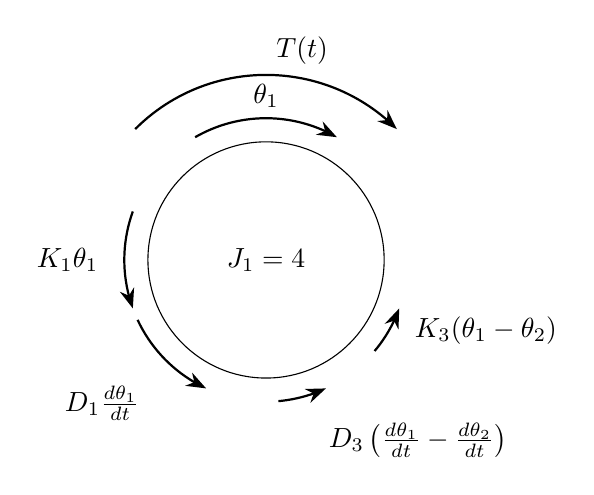
\begin{tikzpicture}[scale=1]
            % Mass J1
            \node[draw, circle, minimum size=3cm] (j1) {$J_1=4$};
            % Positive direction arrow
            \draw[-{Stealth[length=2.5mm]}, thick] (120:1.8cm) arc (120:60:1.8cm) node[midway, above] {$\theta_1$};
            % Applied Torque T(t)
            \draw[-{Stealth[length=2.5mm]}, thick, black!50!black] (135:2.35cm) arc (135:45:2.35cm) node[midway, above right] {$T(t)$};
            % Torques from wall
            \draw[{Stealth[length=2.5mm]}-, thick, black] (200:1.8cm) arc(200:160:1.8cm) node[midway, left=2mm]{$K_1\theta_1$};
            \draw[{Stealth[length=2.5mm]}-, thick, black] (245:1.8cm) arc(245:205:1.8cm) node[midway, below left=2mm]{$D_1\frac{d\theta_1}{dt}$};
            % Torques from J2
            \draw[{Stealth[length=2.5mm]}-, thick, black] (340:1.8cm) arc(340:320:1.8cm) node[midway, right=2mm]{$K_3(\theta_1-\theta_2)$};
            \draw[{Stealth[length=2.5mm]}-, thick, black] (295:1.8cm) arc(295:275:1.8cm) node[midway, below right=2mm]{$D_3\left(\frac{d\theta_1}{dt}-\frac{d\theta_2}{dt}\right)$};
        \end{tikzpicture}
    \end{minipage}
    \hfill
    \begin{minipage}{0.48\textwidth}
        \centering
        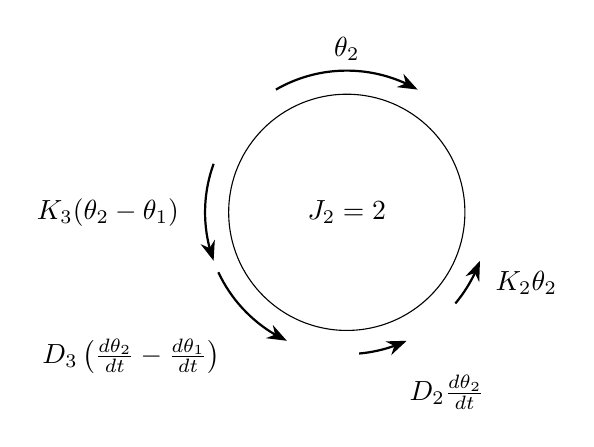
\begin{tikzpicture}[scale=1]
            % Mass J2
            \node[draw, circle, minimum size=3cm] (j2) {$J_2=2$};
            % Positive direction arrow
            \draw[-{Stealth[length=2.5mm]}, thick] (120:1.8cm) arc (120:60:1.8cm) node[midway, above] {$\theta_2$};
            % Torques from J1
            \draw[{Stealth[length=2.5mm]}-, thick, black] (200:1.8cm) arc(200:160:1.8cm) node[midway, left=2mm]{$K_3(\theta_2-\theta_1)$};
            \draw[{Stealth[length=2.5mm]}-, thick, black] (245:1.8cm) arc(245:205:1.8cm) node[midway, below left=2mm]{$D_3\left(\frac{d\theta_2}{dt}-\frac{d\theta_1}{dt}\right)$};
            % Torques from wall
            \draw[{Stealth[length=2.5mm]}-, thick, black] (340:1.8cm) arc(340:320:1.8cm) node[midway, right=2mm]{$K_2\theta_2$};
            \draw[{Stealth[length=2.5mm]}-, thick, black] (295:1.8cm) arc(295:275:1.8cm) node[midway, below right=2mm]{$D_2\frac{d\theta_2}{dt}$};
        \end{tikzpicture}
    \end{minipage}
\end{figure}

\noindent\textbf{Equations of Motion}
\vspace{8pt}

\noindent From the FBDs, we apply Newton's second law for rotation, $\sum \tau = J \frac{d^2\theta}{dt^2}$, to each mass.

\vspace{8pt}
{For Inertia 1 ($J_1$):}
\begin{align*}
% torque balance from FBD
J_1\,\frac{d^2\theta_1}{dt^2}
+ D_1\frac{d\theta_1}{dt}
+ D_3\!\left(\frac{d\theta_1}{dt}-\frac{d\theta_2}{dt}\right)
+ K_1\theta_1
+ K_3\!\left(\theta_1-\theta_2\right)
- T(t) &= 0 \\[4pt]
% collect terms
J_1\,\frac{d^2\theta_1}{dt^2}
+ (D_1+D_3)\frac{d\theta_1}{dt}
+ (K_1+K_3)\theta_1
- D_3\frac{d\theta_2}{dt}
- K_3\theta_2
- T(t) &= 0 \\[4pt]
J_1\,\frac{d^2\theta_1}{dt^2}
+ (D_1+D_3)\frac{d\theta_1}{dt}
+ (K_1+K_3)\theta_1
- D_3\frac{d\theta_2}{dt}
- K_3\theta_2
&= T(t)
\end{align*}

\newpage
{For Inertia 2 ($J_2$):}
\begin{align*}
% torque balance from FBD
J_2\,\frac{d^2\theta_2}{dt^2} 
+ D_2\frac{d\theta_2}{dt}
+ D_3\!\left(\frac{d\theta_2}{dt}-\frac{d\theta_1}{dt}\right)
+ K_2\theta_2
+ K_3\!\left(\theta_2-\theta_1\right) &= 0 \\[4pt]
% collect terms
J_2\,\frac{d^2\theta_2}{dt^2} 
+ (D_2+D_3)\frac{d\theta_2}{dt}
- D_3\frac{d\theta_1}{dt}
+ (K_2+K_3)\theta_2
- K_3\theta_1 &= 0
\end{align*}

\noindent\textbf{Laplace Transform}
\vspace{8pt}

\noindent We take the Laplace transform of the equations, assuming zero initial conditions, and substitute the component values.

\vspace{5pt}
{Substituting values into the transformed equations gives:}
\begin{align}
    (4s^2 + 3s + 2)\Theta_1(s) - (s + 1)\Theta_2(s) &= T(s) \tag{1} \\
    -(s + 1)\Theta_1(s) + (2s^2 + 3s + 2)\Theta_2(s) &= 0 \tag{2}
\end{align}

\noindent\textbf{Solving for the Transfer Function}
\vspace{8pt}

\noindent To find $\dfrac{\Theta_2(s)}{T(s)}$, we must eliminate $\Theta_1(s)$. From equation (2), we can express $\Theta_1(s)$ in terms of $\Theta_2(s)$:
\[
\Theta_1(s) = \frac{2s^2 + 3s + 2}{s + 1} \Theta_2(s)
\]

Now, substitute this into equation (1)
\[
(4s^2 + 3s + 2) \left( \frac{2s^2 + 3s + 2}{s + 1} \Theta_2(s) \right) - (s + 1)\Theta_2(s) = T(s)
\]

Factor out $\Theta_2(s)$:
\[
\left[ \frac{(4s^2 + 3s + 2)(2s^2 + 3s + 2) - (s + 1)^2}{s + 1} \right] \Theta_2(s) = T(s)
\]

Rearrange to find the transfer function $\dfrac{\Theta_2(s)}{T(s)}$:
\[
\frac{\Theta_2(s)}{T(s)} = \frac{s + 1}{(4s^2 + 3s + 2)(2s^2 + 3s + 2) - (s + 1)^2}
\]

Finally, we expand and simplify the denominator:
\begin{align*}
    \text{Term 1: } & (4s^2 + 3s + 2)(2s^2 + 3s + 2) = 8s^4 + 18s^3 + 21s^2 + 12s + 4 \\
    \text{Term 2: } & (s + 1)^2 = s^2 + 2s + 1
\end{align*}

Subtracting the two terms gives the final denominator:
\begin{align*}
&= (8s^4 + 18s^3 + 21s^2 + 12s + 4) - (s^2 + 2s + 1) \\
&= 8s^4 + 18s^3 + 20s^2 + 10s + 3
\end{align*}

The final transfer function is:
\[
\boxed{\frac{\Theta_2(s)}{T(s)} = \frac{s + 1}{8s^4 + 18s^3 + 20s^2 + 10s + 3}}
\]
% Problem 21 - Rotational Mechanical System Transfer Functions
\newpage
  \setcounter{page}{40}  
\noindent\rule{\textwidth}{1pt}
\noindent\textbf{Problem 21} \hfill 
\\ For the given system, find the transfer function $\frac{\theta_1(s)}{T(s)}$.

\begin{figure}[!ht]
\centering
\resizebox{1\textwidth}{!}{%
\begin{circuitikz}
\tikzstyle{every node}=[font=\normalsize]


\filldraw[pattern=bricks, pattern color=black!60] (-0.25,39.25) rectangle (0.5,35.5);
\filldraw[pattern=bricks, pattern color=black!60] (18.75,39.25) rectangle (19.5,35.5);

\draw (4.5,37.25) ellipse (0.25cm and 0.75cm);
\draw [short] (4.5,38) -- (7.25,38);
\draw [short] (4.5,36.5) -- (7.25,36.5);
\draw (11.75,37.25) ellipse (0.25cm and 0.75cm);
\draw [short] (11.75,38) -- (14.5,38);
\draw [short] (11.75,36.5) -- (14.5,36.5);
\node [font=\normalsize] at (13.25,37.25) {$ 3 kg-m^2$};
\node [font=\normalsize] at (6,37.25) {$ 3 kg-m^2$};
\draw [ color={rgb,255:red,46; green,128; blue,163}, ->, >=Stealth] (6,36) .. controls (5.25,36.75) and (5.75,39.75) .. (6.25,38) ;
\draw [ color={rgb,255:red,46; green,128; blue,163}, ->, >=Stealth] (12.5,36) .. controls (11.75,36.75) and (12.25,39.75) .. (12.75,38) ;
\draw [ color={rgb,255:red,46; green,128; blue,163}, ->, >=Stealth] (13.75,36) .. controls (13,36.75) and (13.5,39.75) .. (14,38) ;
\node [font=\normalsize, color={rgb,255:red,46; green,128; blue,163}] at (6,39) {$\theta_1(t)$};
\node [font=\normalsize, color={rgb,255:red,46; green,128; blue,163}] at (12.25,39) {\textit{T(t)}};
\node [font=\normalsize, color={rgb,255:red,46; green,128; blue,163}] at (13.75,39) {$\theta_2(t)$};
\draw [short] (7.25,38) .. controls (7.75,37.75) and (7.5,36.5) .. (7.25,36.5);
\draw [short] (14.5,38) .. controls (15,37.75) and (14.75,36.5) .. (14.5,36.5);
\draw (14.75,37.25) to[short] (15.25,37.25);
\draw (15.25,37.25) to[short] (15.25,37.75);
\draw (15.25,37.75) to[short] (16.25,37.75);
\draw (15.25,37.25) to[short] (15.25,36.75);
\draw (15.25,36.75) to[short] (16.25,36.75);
\draw (15.75,37.5) to[short] (15.75,37);
\draw (15.75,37.25) to[short] (16.75,37.25);
\node [font=\normalsize] at (16,38) {$1 N-m-s/rad$};
\node [font=\normalsize] at (17.50,36.5) {$1 N-m/rad$};
\draw (16.75,37.25) to[L ] (18.75,37.25);
\draw (0.5,37.25) to[short] (1,37.25);
\draw (1,37.25) to[short] (1,37.75);
\draw (1,37.75) to[short] (2,37.75);
\draw (1,37.25) to[short] (1,36.75);
\draw (1,36.75) to[short] (2,36.75);
\draw (1.5,37.5) to[short] (1.5,37);
\draw (1.5,37.25) to[short] (2.5,37.25);
\node [font=\normalsize] at (2,38) {$1 N-m-s/rad$};
\node [font=\normalsize] at (3.2,36.5) {$1 N-m/rad$};
\draw (2.5,37.25) to[L ] (4.5,37.25);
\draw (7.5,37.25) to[short] (8,37.25);
\draw (8,37.25) to[short] (8,37.75);
\draw (8,37.75) to[short] (9,37.75);
\draw (8,37.25) to[short] (8,36.75);
\draw (8,36.75) to[short] (9,36.75);
\draw (8.5,37.5) to[short] (8.5,37);
\draw (8.5,37.25) to[short] (9.5,37.25);
\node [font=\normalsize] at (8.8,38) {$1 N-m-s/rad$};
\node [font=\normalsize] at (10.4,36.5) {$1 N-m/rad$};
\draw (9.5,37.25) to[L ] (11.5,37.25);
\end{circuitikz}
}%
\end{figure}

\noindent\rule{\textwidth}{1pt}

\vspace{12pt}


\noindent\textbf{\textit{Given:}}
\[
J_1,J_2 = 3\, \text{kg}\cdot\text{m}^2
\]
\[
D_1,D_2,D_3 = 1\, \text{N}\cdot\text{m}\cdot\text{s/rad} 
\]
\[
K_1,K_2,K_3 = 1\, \text{N}\cdot\text{m/rad} 
\]

\vspace{1em}
\noindent

\noindent\textbf{\textit{Required:}}
\[
\frac{\theta_1(s)}{F(s)}
\]

\vspace{1.5em}
\noindent\textbf{\textit{Solution:}}

\vspace{8pt}

\noindent\textbf{Free-Body Diagrams (FBDs)}

\vspace{8pt}
\noindent We draw the FBD for each mass. To find the transfer function from the input $T(t)$ on mass $J_2$ to the output $\theta_1(t)$, we assume all other external inputs are zero. Clockwise rotation ($\theta$) is considered positive.

\begin{figure}[h!]
    \centering
    \begin{minipage}{0.48\textwidth}
        \centering
        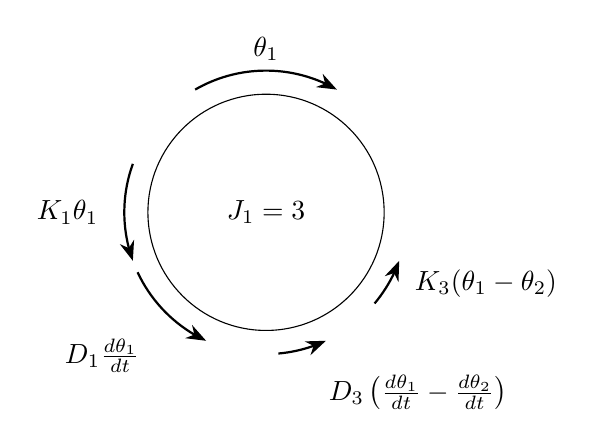
\begin{tikzpicture}[scale=1]
            % Mass J1
            \node[draw, circle, minimum size=3cm] (j1) {$J_1=3$};
            % Positive direction arrow
            \draw[-{Stealth[length=2.5mm]}, thick] (120:1.8cm) arc (120:60:1.8cm) node[midway, above] {$\theta_1$};
            % Torques from wall
            \draw[{Stealth[length=2.5mm]}-, thick, black] (200:1.8cm) arc(200:160:1.8cm) node[midway, left=2mm]{$K_1\theta_1$};
            \draw[{Stealth[length=2.5mm]}-, thick, black] (245:1.8cm) arc(245:205:1.8cm) node[midway, below left=2mm]{$D_1\frac{d\theta_1}{dt}$};
            % Torques from J2
            \draw[{Stealth[length=2.5mm]}-, thick, black] (340:1.8cm) arc(340:320:1.8cm) node[midway, right=2mm]{$K_{3}(\theta_1-\theta_2)$};
            \draw[{Stealth[length=2.5mm]}-, thick, black] (295:1.8cm) arc(295:275:1.8cm) node[midway, below right=2mm]{$D_{3}\left(\frac{d\theta_1}{dt}-\frac{d\theta_2}{dt}\right)$};
        \end{tikzpicture}
    \end{minipage}
    \hfill
    \begin{minipage}{0.48\textwidth}
        \centering
        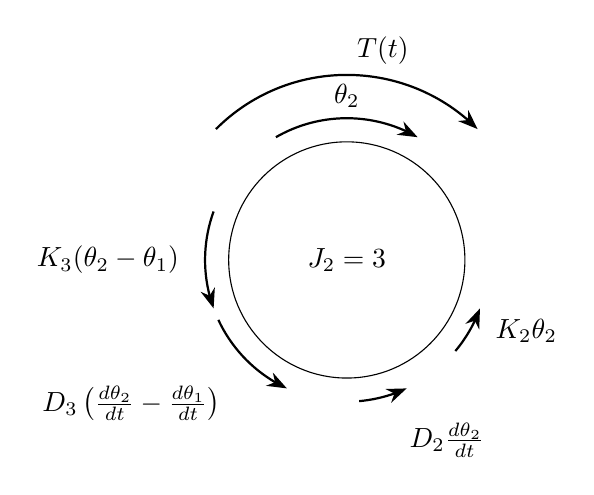
\begin{tikzpicture}[scale=1]
            % Mass J2
            \node[draw, circle, minimum size=3cm] (j2) {$J_2=3$};
            % Positive direction arrow
            \draw[-{Stealth[length=2.5mm]}, thick] (120:1.8cm) arc (120:60:1.8cm) node[midway, above] {$\theta_2$};
            % Applied Torque T(t)
            \draw[-{Stealth[length=2.5mm]}, thick, black!50!black] (135:2.35cm) arc (135:45:2.35cm) node[midway, above right] {$T(t)$};
            % Torques from J1
            \draw[{Stealth[length=2.5mm]}-, thick, black] (200:1.8cm) arc(200:160:1.8cm) node[midway, left=2mm]{$K_{3}(\theta_2-\theta_1)$};
            \draw[{Stealth[length=2.5mm]}-, thick, black] (245:1.8cm) arc(245:205:1.8cm) node[midway, below left=2mm]{$D_{3}\left(\frac{d\theta_2}{dt}-\frac{d\theta_1}{dt}\right)$};
            % Torques from wall
            \draw[{Stealth[length=2.5mm]}-, thick, black] (340:1.8cm) arc(340:320:1.8cm) node[midway, right=2mm]{$K_2\theta_2$};
            \draw[{Stealth[length=2.5mm]}-, thick, black] (295:1.8cm) arc(295:275:1.8cm) node[midway, below right=2mm]{$D_2\frac{d\theta_2}{dt}$};
        \end{tikzpicture}
    \end{minipage}
\end{figure}

\noindent\textbf{Equations of Motion}

\vspace{8pt}

\noindent From the FBDs, we apply Newton's second law for rotation ($\sum \tau = J \frac{d^2\theta}{dt^2}$) to each mass.

{For Inertia 1 ($J_1$):}

\begin{align*}
% torque balance from FBD
J_1\frac{d^2\theta_1}{dt^2}
+ D_1\frac{d\theta_1}{dt}
+ D_3\!\left(\frac{d\theta_1}{dt}-\frac{d\theta_2}{dt}\right)
+ K_1\theta_1
+ K_3\!\left(\theta_1-\theta_2\right) &= 0 \\[4pt]
% collect terms
J_1\frac{d^2\theta_1}{dt^2}
+ (D_1 + D_3)\frac{d\theta_1}{dt}
+ (K_1 + K_3)\theta_1
- D_3\frac{d\theta_2}{dt}
- K_3\theta_2 &= 0
\end{align*}

\newpage
{For Inertia 2 ($J_2$):}
\begin{align*}
% torque balance from FBD (with applied torque)
J_2\frac{d^2\theta_2}{dt^2}
+ D_2\frac{d\theta_2}{dt}
+ D_3\!\left(\frac{d\theta_2}{dt}-\frac{d\theta_1}{dt}\right)
+ K_2\theta_2
+ K_3\!\left(\theta_2-\theta_1\right)
- T(t) &= 0 \\[4pt]
% collect terms
J_2\frac{d^2\theta_2}{dt^2}
+ (D_2 + D_3)\frac{d\theta_2}{dt}
+ (K_2 + K_3)\theta_2
- D_3\frac{d\theta_1}{dt}
- K_3\theta_1
- T(t) &= 0 \\[4pt]
J_2\frac{d^2\theta_2}{dt^2}
+ (D_2 + D_3)\frac{d\theta_2}{dt}
+ (K_2 + K_3)\theta_2
- D_3\frac{d\theta_1}{dt}
- K_3\theta_1
= T(t)
\end{align*}
\noindent\textbf{Laplace Transform}
\vspace{8pt}

\noindent We take the Laplace transform of the equations, assuming zero initial conditions, and substitute the component values.
\vspace{8pt}

{Substituting values into the transformed equations gives:}
\begin{align}
    (3s^2 + 2s + 2)\Theta_1(s) - (s + 1)\Theta_2(s) &= 0 \tag{1} \\
    -(s + 1)\Theta_1(s) + (3s^2 + 2s + 2)\Theta_2(s) &= T(s) \tag{2}
\end{align}

\noindent\textbf{Solving for the Transfer Function}
\vspace{8pt}

\noindent To find $\dfrac{\Theta_1(s)}{T(s)}$, we must eliminate $\Theta_2(s)$. From equation (1,) we can express $\Theta_2(s)$ in terms of $\Theta_1(s)$:
\[
\Theta_2(s) = \frac{3s^2 + 2s + 2}{s + 1} \Theta_1(s)
\]

Now, substitute this into equation (2):
\[
-(s + 1)\Theta_1(s) + (3s^2 + 2s + 2) \left( \frac{3s^2 + 2s + 2}{s + 1} \Theta_1(s) \right) = T(s)
\]

Factor out $\Theta_1(s)$:
\[
\left[ \frac{-(s + 1)^2 + (3s^2 + 2s + 2)^2}{s + 1} \right] \Theta_1(s) = T(s)
\]

Rearrange to find the transfer function $\dfrac{\Theta_1(s)}{T(s)}$:
\[
\frac{\Theta_1(s)}{T(s)} = \frac{s + 1}{(3s^2 + 2s + 2)^2 - (s + 1)^2}
\]

Finally, we expand and simplify the denominator:
\begin{align*}
    \text{Term 1: } & (3s^2 + 2s + 2)^2 = 9s^4 + 12s^3 + 16s^2 + 8s + 4 \\
    \text{Term 2: } & (s + 1)^2 = s^2 + 2s + 1
\end{align*}

Subtracting the two terms gives the final denominator:
\begin{align*}
&= (9s^4 + 12s^3 + 16s^2 + 8s + 4) - (s^2 + 2s + 1) \\
&= 9s^4 + 12s^3 + 15s^2 + 6s + 3
\end{align*}

The final transfer function is:
\[
\boxed{\frac{\Theta_1(s)}{T(s)} = \frac{s + 1}{9s^4 + 12s^3 + 15s^2 + 6s + 3}}
\]




% Problem 22 - Rotational Mechanical System Transfer Functions
\newpage
% command for new page 
  \setcounter{page}{42}  
\noindent\rule{\textwidth}{1pt}
\noindent\textbf{Problem 22} \hfill 
%palagay ulit dito 'yung problem statement
\\ For the given system, find the transfer function $\frac{\theta_2(s)}{T(s)}$.

\begin{figure}[!ht]
\centering
\resizebox{1\textwidth}{!}{%
\begin{circuitikz}
\tikzstyle{every node}=[font=\LARGE]


\filldraw[pattern=bricks, pattern color=black!60] (17.75,34.25) rectangle (18.25,30.5);
\filldraw[pattern=bricks, pattern color=black!60] (5.75,28.5) rectangle (9.5,28);

\draw (13.75,32.5) to[short] (14.25,32.5);
\draw (14.25,32.5) to[short] (14.25,33);
\draw (14.25,33) to[short] (15.25,33);
\draw (14.25,32.5) to[short] (14.25,32);
\draw (14.25,32) to[short] (15.25,32);
\draw (14.75,32.75) to[short] (14.75,32.25);
\draw (14.75,32.5) to[short] (15.75,32.5);
\node [font=\normalsize] at (14.75,33.25) {$1 N-m-s/rad$};
\node [font=\normalsize] at (16,31.75) {$1 N-m/rad$};
\draw (15.75,32.5) to[L ] (17.75,32.5);
\draw (9.25,33.25) to[L ] (11.25,33.25);
\draw (9.25,31.75) to[short] (9.75,31.75);
\draw (9.75,31.75) to[short] (9.75,32.25);
\draw (9.75,32.25) to[short] (10.75,32.25);
\draw (9.75,31.75) to[short] (9.75,31.25);
\draw (9.75,31.25) to[short] (10.75,31.25);
\draw (10.25,32) to[short] (10.25,31.5);
\draw (10.25,31.75) to[short] (11.25,31.75);
\draw [short] (8.25,33.25) -- (9.25,33.25);
\draw [short] (8.25,33.25) -- (8.25,31.75);
\draw [short] (8.25,31.75) -- (9.25,31.75);
\draw [short] (11.25,33.25) -- (12.25,33.25);
\draw [short] (12.25,33.25) -- (12.25,31.75);
\draw [short] (11.25,31.75) -- (12.25,31.75);
\draw (4,32.5) ellipse (0.25cm and 0.75cm);
\draw [short] (4,33.25) -- (6.75,33.25);
\draw [short] (4,31.75) -- (6.75,31.75);
\node [font=\normalsize] at (5.5,32.5) {$ 1 kg-m^2$};
\draw [ color={rgb,255:red,46; green,128; blue,163}, ->, >=Stealth] (4,31.25) .. controls (3.25,32) and (3.75,35) .. (4.25,33.25) ;
\node [font=\normalsize, color={rgb,255:red,46; green,128; blue,163}] at (4.5,34.25) {$\theta_1(t)$};
\draw [short] (6.75,33.25) .. controls (7.25,33) and (7,31.75) .. (6.75,31.75);
\draw (7,30.5) to[short] (7,31);
\draw (8,30) to[short] (8,31);
\draw (7,30.5) to[short] (7,30);
\draw (7,30) to[short] (8,30);
\draw (7.25,30.5) to[short] (7.75,30.5);
\draw (7.5,32.5) to[short] (7.5,30.5);
\draw [short] (7,32.5) -- (8.25,32.5);
\draw [short] (12.25,32.5) -- (13.75,32.5);
\draw [short] (2,32.5) -- (4,32.5);
\draw [ color={rgb,255:red,46; green,128; blue,163}, ->, >=Stealth] (3.25,31.25) .. controls (2.5,32) and (3,35) .. (3.5,33.25) ;
\node [font=\normalsize, color={rgb,255:red,46; green,128; blue,163}] at (3.25,34.25) {\textit{T(t)}};
\node [font=\normalsize] at (10.25,33.75) {$1 N-m/rad$};
\node [font=\normalsize] at (10.25,31) {$1 N-m-s/rad$};
\node [font=\normalsize, color={rgb,255:red,46; green,128; blue,163}] at (13.5,34.25) {$\theta_2(t)$};
\draw [ color={rgb,255:red,46; green,128; blue,163}, ->, >=Stealth] (13.5,31.25) .. controls (12.75,32) and (13.25,35) .. (13.75,33.25) ;
\node [font=\normalsize] at (5,30.5) {$1 N-m-s/rad$};
\draw (7.5,28.5) to[L ] (7.5,30);
\node [font=\normalsize] at (9,29) {$1 N-m/rad$};
\end{circuitikz}
}%
\end{figure}

\noindent\rule{\textwidth}{1pt}

\vspace{12pt}


\noindent\textbf{\textit{Given:}}
\[
J_1 = 1\, \text{kg}\cdot\text{m}^2, J_2 = 0 \ (Mass less\ node)
\]
\[
B_1,B_2,B_3 = 1\, \text{N}\cdot\text{m}\cdot\text{s/rad} 
\]
\[
K_1,K_2,K_3 = 1\, \text{N}\cdot\text{m/rad} 
\]

\vspace{1em}
\noindent

\noindent\textbf{\textit{Required:}}
\[
\frac{\theta_2(s)}{T(s)}
\]

\vspace{1.5em}
\noindent\textbf{\textit{Solution:}}

\vspace{8pt}

\noindent\textbf{Free-Body Diagrams (FBDs)}
\vspace{8pt}

\noindent  Note that the damper $D_{3}$ does not create a torque on $J_1$, and three components create torques on Node $\theta_2$ relative to ground.

\begin{figure}[h!]
    \centering
    \begin{minipage}{0.48\textwidth}
        \centering
        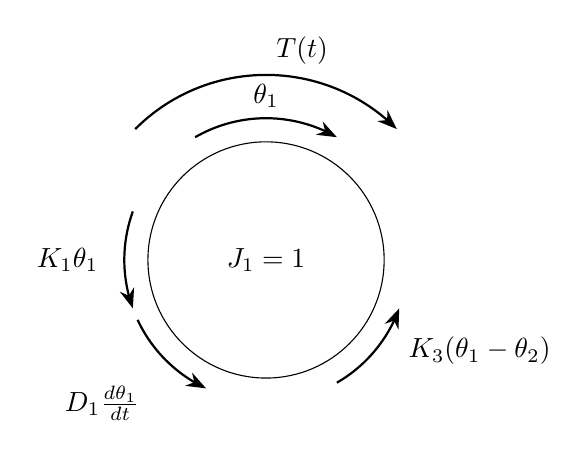
\begin{tikzpicture}[scale=1]
            % Mass J1
            \node[draw, circle, minimum size=3cm] (j1) {$J_1=1$};
            % Positive direction arrow
            \draw[-{Stealth[length=2.5mm]}, thick] (120:1.8cm) arc (120:60:1.8cm) node[midway, above] {$\theta_1$};
            % Applied Torque T(t)
            \draw[-{Stealth[length=2.5mm]}, thick, black!50!black] (135:2.35cm) arc (135:45:2.35cm) node[midway, above right] {$T(t)$};
            % Torques from wall
            \draw[{Stealth[length=2.5mm]}-, thick, black] (200:1.8cm) arc(200:160:1.8cm) node[midway, left=2mm]{$K_1\theta_1$};
            \draw[{Stealth[length=2.5mm]}-, thick, black] (245:1.8cm) arc(245:205:1.8cm) node[midway, below left=2mm]{$D_1\frac{d\theta_1}{dt}$};
            % Coupling Torque (Spring ONLY)
            \draw[{Stealth[length=2.5mm]}-, thick, black] (340:1.8cm) arc(340:300:1.8cm) node[midway, right=3mm]{$K_{3}(\theta_1-\theta_2)$};
        \end{tikzpicture}
    \end{minipage}
    \hfill
    \begin{minipage}{0.48\textwidth}
        \centering
        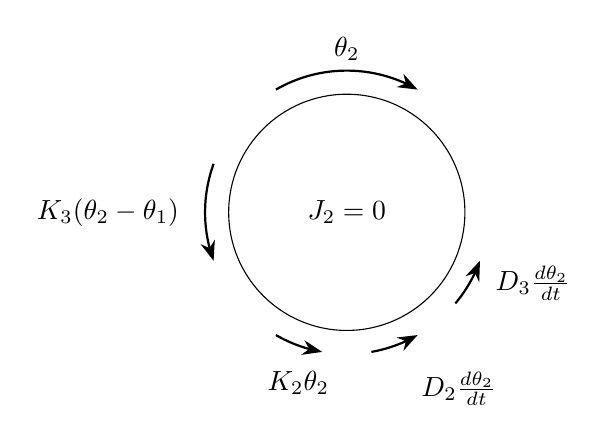
\begin{tikzpicture}[scale=1]
            % Node 2
            \node[draw, circle, minimum size=3cm] (j2) {$J_2=0$};
            % Positive direction arrow
            \draw[-{Stealth[length=2.5mm]}, thick] (120:1.8cm) arc (120:60:1.8cm) node[midway, above] {$\theta_2$};
            % Coupling Torque (Spring ONLY)
            \draw[{Stealth[length=2.5mm]}-, thick, black] (200:1.8cm) arc(200:160:1.8cm) node[midway, left=2mm]{$K_{3}(\theta_2-\theta_1)$};
            % Ground Torques (3 elements)
            \draw[{Stealth[length=2.5mm]}-, thick, black] (340:1.8cm) arc(340:320:1.8cm) node[midway, right=2mm]{$D_{3}\frac{d\theta_2}{dt}$};
            \draw[{Stealth[length=2.5mm]}-, thick, black] (300:1.8cm) arc(300:280:1.8cm) node[midway, below right=2mm]{$D_2\frac{d\theta_2}{dt}$};
            \draw[{Stealth[length=2.5mm]}-, thick, black] (260:1.8cm) arc(260:240:1.8cm) node[midway, below=2mm]{$K_2\theta_2$};
        \end{tikzpicture}
    \end{minipage}
\end{figure}

\noindent\textbf{Equations of Motion}

\vspace{8pt}

\noindent From the FBDs, we write the torque-balance equations for each node.

\vspace{8pt}
{For Node 1 ($J_1$):}
\begin{align*}
    J_1 \frac{d^2\theta_1}{dt^2} + D_1 \frac{d\theta_1}{dt} + K_1 \theta_1 + K_{3}(\theta_1 - \theta_2) &= T(t) \\
    J_1 \frac{d^2\theta_1}{dt^2} + D_1 \frac{d\theta_1}{dt} + (K_1 + K_{3})\theta_1 - K_{3}\theta_2 &= T(t)
\end{align*}

{For Node 2 (massless, $J_2 = 0$):}
\begin{align*}
    K_{3}(\theta_2 - \theta_1) + D_{3} \frac{d\theta_2}{dt} + D_2 \frac{d\theta_2}{dt} + K_2 \theta_2 &= 0 \\
    -K_{3}\theta_1 + (D_2 + D_{3})\frac{d\theta_2}{dt} + (K_2 + K_{3})\theta_2 &= 0
\end{align*}

\noindent\textbf{Laplace Transform}

\vspace{8pt}

\noindent We take the Laplace transform of the equations, assuming zero initial conditions, and substitute the component values.

\vspace{8pt}
{Equation 1 (Node 1):}
\begin{align}
    (s^2 + s + 2)\Theta_1(s) - \Theta_2(s) &= T(s) \tag{1}
\end{align}

{Equation 2 (Node 2):}
\begin{align}
    -\Theta_1(s) + (2s + 2)\Theta_2(s) &= 0 \tag{2}
\end{align}


\noindent\textbf{Solving for the Transfer Function}
\vspace{8pt}

To find $\dfrac{\Theta_2(s)}{T(s)}$, we first solve equation (2) for $\Theta_1(s)$:
\[
\Theta_1(s) = (2s + 2)\Theta_2(s)
\]

Now, substitute this expression for $\Theta_1(s)$ into equation (1):
\[
(s^2 + s + 2)\left[ (2s + 2)\Theta_2(s) \right] - \Theta_2(s) = T(s)
\]

Factor out $\Theta_2(s)$:
\[
\left[ (s^2 + s + 2)(2s + 2) - 1 \right] \Theta_2(s) = T(s)
\]

Expand the polynomial in the brackets:
\begin{align*}
(s^2 + s + 2)(2s + 2) &= 2s^3 + 2s^2 + 2s^2 + 2s + 4s + 4 \\
&= 2s^3 + 4s^2 + 6s + 4
\end{align*}

Substitute the expanded term back into the equation:
\begin{align*}
[ (2s^3 + 4s^2 + 6s + 4) - 1 ] \Theta_2(s) &= T(s) \\
(2s^3 + 4s^2 + 6s + 3) \Theta_2(s) &= T(s)
\end{align*}

The final transfer function is:
\[
\boxed{\frac{\Theta_2(s)}{T(s)} = \frac{1}{2s^3 + 4s^2 + 6s + 3}}
\]



% Problem 23 - Rotational Mechanical System Transfer Functions

\newpage
% command for new page 
  \setcounter{page}{44}  
\noindent\rule{\textwidth}{1pt}
\noindent\textbf{Problem 23} \hfill 
%palagay ulit dito 'yung problem statement
\\ For the given system, find the transfer function $\frac{\theta_2(s)}{T(s)}$.

\begin{figure}[!ht]
\centering
\resizebox{1\textwidth}{!}{%
\begin{circuitikz}
\tikzstyle{every node}=[font=\normalsize]


\filldraw [pattern=bricks, pattern color=black!60] (-0.25,39.25) rectangle (0.5,35.5);
\filldraw [pattern=bricks, pattern color=black!60] (17.75,39.25) rectangle (18.5,35.5);

\node [font=\small] at (1.8,36) {$1 N-m-s/rad$};
\draw  (2.75,37.25) ellipse (0.25cm and 0.75cm);
\draw [short] (2.75,38) -- (5.5,38);
\draw [short] (2.75,36.5) -- (5.5,36.5);
\draw  (7.75,37.25) ellipse (0.25cm and 0.75cm);
\draw [short] (7.75,38) -- (10.5,38);
\draw [short] (7.75,36.5) -- (10.5,36.5);
\draw (5.75,37.75) to [short] (6.25,37.75);
\draw (6.25,37.75) to [short] (6.25,38.25);
\draw (6.25,38.25) to [short] (7.25,38.25);
\draw (6.25,37.75) to [short] (6.25,37.25);
\draw (6.25,37.25) to [short] (7.25,37.25);
\draw (6.75,38) to [short] (6.75,37.5);
\draw (6.75,37.75) to [short] (7.75,37.75);
\draw (5.75,36.75) to [L ] (7.75,36.75);
\node [font=\normalsize] at (9.25,37.25) {$ 1 kg-m^2$};
\node [font=\normalsize] at (4.25,37.25) {$ 1 kg-m^2$};
\node [font=\small] at (6.75,38.5) {$1 N-m-s/rad$};
\node [font=\small] at (6.5,36.25) {$1 N-m/rad$};
\draw [ color={rgb,255:red,46; green,128; blue,163}, ->, >=Stealth] (2.75,36) .. controls (2,36.75) and (2.5,39.75) .. (3,38) ;
\draw [ color={rgb,255:red,46; green,128; blue,163}, ->, >=Stealth] (5.5,36) .. controls (4.75,36.75) and (5.25,39.75) .. (5.75,38) ;
\draw [ color={rgb,255:red,46; green,128; blue,163}, ->, >=Stealth] (8.25,36) .. controls (7.5,36.75) and (8,39.75) .. (8.5,38) ;
\node [font=\normalsize, color={rgb,255:red,46; green,128; blue,163}] at (2.75,39) {$\theta_1(t)$};
\node [font=\normalsize, color={rgb,255:red,46; green,128; blue,163}] at (5.25,39) {\textit{T(t)}};
\node [font=\normalsize, color={rgb,255:red,46; green,128; blue,163}] at (8.25,39) {$\theta_2(t)$};
\draw [short] (5.5,38) .. controls (6,37.75) and (5.75,36.5) .. (5.5,36.5);
\draw [short] (10.5,38) .. controls (11,37.75) and (10.75,36.5) .. (10.5,36.5);
\draw (0.5,37.25) to [short] (1,37.25);
\draw (1,37.25) to [short] (1,37.75);
\draw (1,37.75) to [short] (2,37.75);
\draw (1,37.25) to [short] (1,36.75);
\draw (1,36.75) to [short] (2,36.75);
\draw (1.5,37.5) to [short] (1.5,37);
\draw (1.5,37.25) to [short] (2.5,37.25);
\draw  (12.75,37.25) ellipse (0.25cm and 0.75cm);
\draw [short] (12.75,38) -- (15.5,38);
\draw [short] (12.75,36.5) -- (15.5,36.5);
\draw (10.75,37.75) to [short] (11.25,37.75);
\draw (11.25,37.75) to [short] (11.25,38.25);
\draw (11.25,38.25) to [short] (12.25,38.25);
\draw (11.25,37.75) to [short] (11.25,37.25);
\draw (11.25,37.25) to [short] (12.25,37.25);
\draw (11.75,38) to [short] (11.75,37.5);
\draw (11.75,37.75) to [short] (12.75,37.75);
\draw (10.75,36.75) to [L ] (12.75,36.75);
\node [font=\normalsize] at (14.25,37.25) {$ 1 kg-m^2$};
\node [font=\small] at (11.75,38.5) {$1 N-m-s/rad$};
\node [font=\small] at (11.5,36.25) {$1 N-m/rad$};
\draw [ color={rgb,255:red,46; green,128; blue,163}, ->, >=Stealth] (13.25,36) .. controls (12.5,36.75) and (13,39.75) .. (13.5,38) ;
\node [font=\normalsize, color={rgb,255:red,46; green,128; blue,163}] at (13.25,39) {$\theta_3(t)$};
\draw [short] (15.5,38) .. controls (16,37.75) and (15.75,36.5) .. (15.5,36.5);
\draw (15.75,37.25) to [short] (16.25,37.25);
\draw (16.25,37.25) to [short] (16.25,37.75);
\draw (16.25,37.75) to [short] (17.25,37.75);
\draw (16.25,37.25) to [short] (16.25,36.75);
\draw (16.25,36.75) to [short] (17.25,36.75);
\draw (16.75,37.5) to [short] (16.75,37);
\draw (16.75,37.25) to [short] (17.75,37.25);
\node [font=\small] at (16.1,36) {$1 N-m-s/rad$};
\end{circuitikz}
}%
\end{figure}

\noindent\rule{\textwidth}{1pt}

\vspace{12pt}


\noindent\textbf{\textit{Given:}}
\[
J_1, J_2,J_3 = 1\, \text{kg}\cdot\text{m}^2
\]
\[
B_1,B_{12},B_{23} B_3 = 1\, \text{N}\cdot\text{m}\cdot\text{s/rad} 
\]
\[
K_1,K_{12},K_{23} K_3 = 1\, \text{N}\cdot\text{m/rad} 
\]

\vspace{1em}
\noindent

\noindent\textbf{\textit{Required:}}
\[
\frac{\theta_2(s)}{T(s)}
\]

\vspace{1.5em}
\noindent\textbf{\textit{Solution:}}

\vspace{8pt}

\noindent\textbf{Free-Body Diagrams (FBDs)}

\vspace{8pt}

% ---- J1 ----
\begin{figure}[h!]
  \centering
  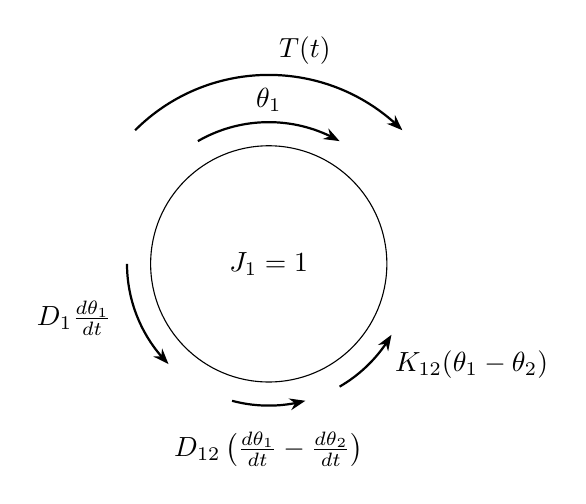
\begin{tikzpicture}[scale=1, every node/.style={font=\normalsize}]
    \node[draw, circle, minimum size=3cm] (j1) {$J_1=1$};
    \draw[-{Stealth[length=2mm]}, thick] (120:1.8cm) arc (120:60:1.8cm) node[midway, above] {$\theta_1$};
    \draw[-{Stealth[length=2mm]}, thick, black!50!black] (135:2.40cm) arc (135:45:2.40cm) node[midway, above right] {$T(t)$};
    \draw[{Stealth[length=2mm]}-, thick, black] (225:1.8cm) arc(225:180:1.8cm) node[midway, left=2mm]{$D_1\frac{d\theta_1}{dt}$};
    \draw[{Stealth[length=2mm]}-, thick, black] (330:1.8cm) arc(330:300:1.8cm) node[midway, right=2mm]{$K_{12}(\theta_1-\theta_2)$};
    \draw[{Stealth[length=2mm]}-, thick, black] (285:1.8cm) arc(285:255:1.8cm) node[midway, below=2mm]{$D_{12}\left(\frac{d\theta_1}{dt}-\frac{d\theta_2}{dt}\right)$};
  \end{tikzpicture}
\end{figure}

\vspace{5pt}

{For Mass 1 ($J_1$):}

\begin{align*}
% torque balance
J_1\frac{d^2\theta_1}{dt^2}
+ D_1\frac{d\theta_1}{dt}
+ D_{12}\!\left(\frac{d\theta_1}{dt}-\frac{d\theta_2}{dt}\right)
+ K_{12}\!\left(\theta_1-\theta_2\right)
- T(t) &= 0 \\[4pt]
% collect terms
J_1\frac{d^2\theta_1}{dt^2}
+ (D_1+D_{12})\frac{d\theta_1}{dt}
+ K_{12}\theta_1
- D_{12}\frac{d\theta_2}{dt}
- K_{12}\theta_2
- T(t) &= 0 \\[4pt]
J_1\frac{d^2\theta_1}{dt^2}
+ (D_1+D_{12})\frac{d\theta_1}{dt}
+ K_{12}\theta_1
- D_{12}\frac{d\theta_2}{dt}
- K_{12}\theta_2
&= T(t)
\end{align*}

\newpage
\begin{figure}[h!]
  \centering
  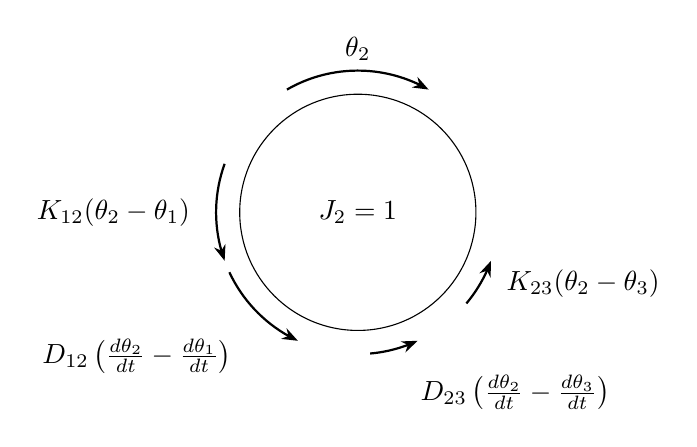
\begin{tikzpicture}[scale=1, every node/.style={font=\normalsize}]
    \node[draw, circle, minimum size=3cm] (j2) {$J_2=1$};
    \draw[-{Stealth[length=2mm]}, thick] (120:1.8cm) arc (120:60:1.8cm) node[midway, above] {$\theta_2$};
    \draw[{Stealth[length=2mm]}-, thick, black] (200:1.8cm) arc(200:160:1.8cm) node[midway, left=2mm]{$K_{12}(\theta_2-\theta_1)$};
    \draw[{Stealth[length=2mm]}-, thick, black] (245:1.8cm) arc(245:205:1.8cm) node[midway, below left=2mm]{$D_{12}\left(\frac{d\theta_2}{dt}-\frac{d\theta_1}{dt}\right)$};
    \draw[{Stealth[length=2mm]}-, thick, black] (340:1.8cm) arc(340:320:1.8cm) node[midway, right=2mm]{$K_{23}(\theta_2-\theta_3)$};
    \draw[{Stealth[length=2mm]}-, thick, black] (295:1.8cm) arc(295:275:1.8cm) node[midway, below right=2mm]{$D_{23}\left(\frac{d\theta_2}{dt}-\frac{d\theta_3}{dt}\right)$};
  \end{tikzpicture}
\end{figure}
\vspace{5pt}

{For Mass 2 ($J_2$):}
\begin{align*}
% torque balance about $J_2$
J_2\frac{d^2\theta_2}{dt^2}
+ D_{12}\!\left(\frac{d\theta_2}{dt}-\frac{d\theta_1}{dt}\right)
+ K_{12}\!\left(\theta_2-\theta_1\right)
+ D_{23}\!\left(\frac{d\theta_2}{dt}-\frac{d\theta_3}{dt}\right)
+ K_{23}\!\left(\theta_2-\theta_3\right) &= 0 \\[4pt]
% collect like terms
J_2\frac{d^2\theta_2}{dt^2}
+ (D_{12}+D_{23})\frac{d\theta_2}{dt}
- D_{12}\frac{d\theta_1}{dt}
- D_{23}\frac{d\theta_3}{dt}
+ (K_{12}+K_{23})\theta_2
- K_{12}\theta_1
- K_{23}\theta_3 &= 0
\end{align*}

\begin{figure}[h!]
  \centering
  \hspace*{-20mm}
  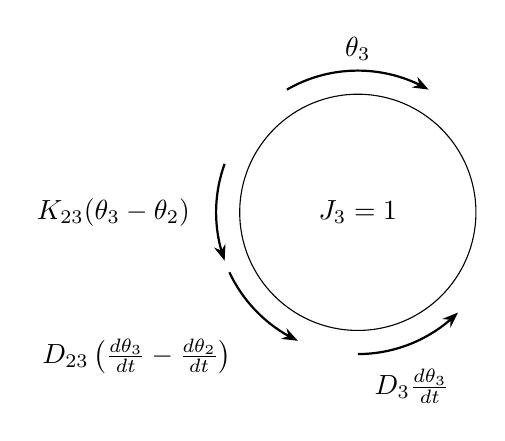
\begin{tikzpicture}[scale=1, every node/.style={font=\normalsize}]
    \node[draw, circle, minimum size=3cm] (j3) {$J_3=1$};
      \draw[-{Stealth[length=2mm]}, thick] (120:1.8cm) arc (120:60:1.8cm) node[midway, above] {$\theta_3$};
      \draw[{Stealth[length=2mm]}-, thick, black] (200:1.8cm) arc(200:160:1.8cm) node[midway, left=2mm]{$K_{23}(\theta_3-\theta_2)$};
      \draw[{Stealth[length=2mm]}-, thick, black] (245:1.8cm) arc(245:205:1.8cm) node[midway, below left=2mm]{$D_{23}\left(\frac{d\theta_3}{dt}-\frac{d\theta_2}{dt}\right)$};
      \draw[{Stealth[length=2mm]}-, thick, black] (315:1.8cm) arc(315:270:1.8cm) node[midway, below=2mm]{$D_3\frac{d\theta_3}{dt}$};
  \end{tikzpicture}
\end{figure}

{For Mass 3 ($J_3$):}
\begin{align*}
% torque balance about $J_3$
J_3\frac{d^2\theta_3}{dt^2}
+ D_3\frac{d\theta_3}{dt}
+ D_{23}\!\left(\frac{d\theta_3}{dt}-\frac{d\theta_2}{dt}\right)
+ K_{23}\!\left(\theta_3-\theta_2\right) &= 0 \\[4pt]
% collect like terms
J_3\frac{d^2\theta_3}{dt^2}
+ (D_3+D_{23})\frac{d\theta_3}{dt}
- D_{23}\frac{d\theta_2}{dt}
+ K_{23}\theta_3
- K_{23}\theta_2 &= 0
\end{align*}


\noindent\textbf{Laplace Transform}
\vspace{8pt}

\noindent We take the Laplace transform and define impedance terms to simplify the notation.

\vspace{5pt}
{Impedance Definitions:}
\begin{align*}
    Z_1(s) &= J_1s^2 + (B_1+B_{12})s + K_{12} = s^2 + 2s + 1 = (s+1)^2 \\
    Z_2(s) &= J_2s^2 + (B_{12}+B_{23})s + (K_{12}+K_{23}) = s^2 + 2s + 2 \\
    Z_3(s) &= J_3s^2 + (B_3+B_{23})s + K_{23} = s^2 + 2s + 1 = (s+1)^2 \\
    Z_{12}(s) &= B_{12}s + K_{12} = s+1 \\
    Z_{23}(s) &= B_{23}s + K_{23} = s+1
\end{align*}

{System of Equations in the s-Domain:}
\begin{align}
    Z_1(s)\Theta_1(s) - Z_{12}(s)\Theta_2(s) &= T(s) \tag{1}\\
    -Z_{12}(s)\Theta_1(s) + Z_2(s)\Theta_2(s) - Z_{23} (s)\Theta_3(s) &= 0 \tag{2}\\
    -Z_{23}(s)\Theta_2(s) + Z_3(s)\Theta_3(s) &= 0 \tag{3}
\end{align}

\newpage
\noindent\textbf{Solving for the Transfer Function}

\vspace{8pt}

We use Cramer's rule on the 3x3 system to solve for $\Theta_2(s)$.
\vspace{5pt}

{System Determinant ($\Delta(s)$):}
\begin{align*}
    \Delta(s) &= Z_1(Z_2Z_3 - Z_{23}^2) - Z_{12}^2Z_3 \\
    &= (s+1)^2(s^2+2s+2)(s+1)^2 - (s+1)^2(s+1)^2 - (s+1)^2(s+1)^2 \\
    &= (s+1)^4(s^2+2s+2) - 2(s+1)^4 \\
    &= (s+1)^4[(s^2+2s+2)-2] = s(s+2)(s+1)^4
\end{align*}

{Numerator for $\Theta_2$ ($N_2(s)$):}
\[
N_2(s) = \begin{vmatrix} Z_1 & T(s) & 0 \\ -Z_{12} & 0 & -Z_{23} \\ 0 & 0 & Z_3 \end{vmatrix}
\]

Expanding along the third row:
\begin{align*}
    N_2(s) &= Z_3 \cdot \begin{vmatrix} Z_1 & T(s) \\ -Z_{12} & 0 \end{vmatrix} \\
    &= Z_3 [Z_1(0) - T(s)(-Z_{12})] = T(s) \cdot Z_{12}Z_3 \\
    &= T(s) \cdot (s+1)(s+1)^2 = T(s)(s+1)^3
\end{align*}

{Final Transfer Function:}
\[
\frac{\Theta_2(s)}{T(s)} = \frac{N_2(s)/T(s)}{\Delta(s)} = \frac{(s+1)^3}{s(s+2)(s+1)^4}
\]

After cancelling the common terms, we get:
\[
\boxed{\frac{\Theta_2(s)}{T(s)} = \frac{1}{s(s+1)(s+2)}}
\]



% Problem 24 - Rotational Mechanical System Transfer Functions
\newpage
  \setcounter{page}{47}  
\noindent\rule{\textwidth}{1pt}
\noindent\textbf{Problem 24} \hfill 
\\ For the given system, find the transfer function $\frac{\theta_1(s)}{T(s)}$.

\begin{figure}[!ht]
\centering
\resizebox{0.9\textwidth}{!}{%
\begin{circuitikz}
\tikzstyle{every node}=[font=\normalsize]


\filldraw [pattern=bricks, pattern color=black!60] (-0.5,39.25) rectangle (0.25,35.5);
\filldraw [pattern=bricks, pattern color=black!60] (17.75,39.25) rectangle (18.5,35.5);

\draw (2.75,37.25) ellipse (0.25cm and 0.75cm);
\draw [short] (2.75,38) -- (5.5,38);
\draw [short] (2.75,36.5) -- (5.5,36.5);
\draw (7.75,37.25) ellipse (0.25cm and 0.75cm);
\draw [short] (7.75,38) -- (10.5,38);
\draw [short] (7.75,36.5) -- (10.5,36.5);
\draw (5.75,37.25) to [L ] (7.75,37.25);
\node [font=\normalsize] at (9.25,37.25) {$ 2 kg-m^2$};
\node [font=\normalsize] at (4.25,37.25) {$ 2 kg-m^2$};
\node [font=\small] at (6.75,36.75) {$1 N-m/rad$};
\draw [ color={rgb,255:red,46; green,128; blue,163}, ->, >=Stealth] (3.25,36) .. controls (2.5,36.75) and (3,39.75) .. (3.5,38) ;
\draw [ color={rgb,255:red,46; green,128; blue,163}, ->, >=Stealth] (8,36) .. controls (7.25,36.75) and (7.75,39.75) .. (8.25,38) ;
\draw [ color={rgb,255:red,46; green,128; blue,163}, ->, >=Stealth] (8.75,36) .. controls (8,36.75) and (8.5,39.75) .. (9,38) ;
\node [font=\normalsize, color={rgb,255:red,46; green,128; blue,163}] at (3.25,39) {$\theta_1(t)$};
\node [font=\normalsize, color={rgb,255:red,46; green,128; blue,163}] at (7.75,39) {\textit{T(t)}};
\node [font=\normalsize, color={rgb,255:red,46; green,128; blue,163}] at (8.75,39) {$\theta_2(t)$};
\draw [short] (5.5,38) .. controls (6,37.75) and (5.75,36.5) .. (5.5,36.5);
\draw [short] (10.5,38) .. controls (11,37.75) and (10.75,36.5) .. (10.5,36.5);
\draw (12.75,37.25) ellipse (0.25cm and 0.75cm);
\draw [short] (12.75,38) -- (15.5,38);
\draw [short] (12.75,36.5) -- (15.5,36.5);
\draw (10.75,37.75) to [short] (11.25,37.75);
\draw (11.25,37.75) to [short] (11.25,38.25);
\draw (11.25,38.25) to [short] (12.25,38.25);
\draw (11.25,37.75) to [short] (11.25,37.25);
\draw (11.25,37.25) to [short] (12.25,37.25);
\draw (11.75,38) to [short] (11.75,37.5);
\draw (11.75,37.75) to [short] (12.75,37.75);
\draw (10.75,36.75) to [L ] (12.75,36.75);
\node [font=\normalsize] at (14.25,37.25) {$ 4 kg-m^2$};
\node [font=\small] at (11.75,38.5) {$3 N-m-s/rad$};
\node [font=\small] at (11.5,36.25) {$3 N-m/rad$};
\draw [ color={rgb,255:red,46; green,128; blue,163}, ->, >=Stealth] (13.25,36) .. controls (12.5,36.75) and (13,39.75) .. (13.5,38) ;
\node [font=\normalsize, color={rgb,255:red,46; green,128; blue,163}] at (13.25,39) {$\theta_3(t)$};
\draw [short] (15.5,38) .. controls (16,37.75) and (15.75,36.5) .. (15.5,36.5);
\draw (15.75,37.25) to [short] (16.25,37.25);
\draw (16.25,37.25) to [short] (16.25,37.75);
\draw (16.25,37.75) to [short] (17.25,37.75);
\draw (16.25,37.25) to [short] (16.25,36.75);
\draw (16.25,36.75) to [short] (17.25,36.75);
\draw (16.75,37.5) to [short] (16.75,37);
\draw (16.75,37.25) to [short] (17.75,37.25);
\node [font=\small] at (16.30,38.25) {$5 N-m-s/rad$};
\draw (0.25,37.75) to [short] (1.25,37.75);
\draw (1.25,37.75) to [short] (1.25,38.25);
\draw (1.25,38.25) to [short] (2.25,38.25);
\draw (1.25,37.75) to [short] (1.25,37.25);
\draw (1.25,37.25) to [short] (2.25,37.25);
\draw (1.75,38) to [short] (1.75,37.5);
\draw (1.75,37.75) to [short] (2.75,37.75);
\draw (0.25,36.75) to [L ] (2.75,36.75);
\node [font=\small] at (1.55,38.5) {$1 N-m-s/rad$};
\node [font=\small] at (1.6,36.25) {$1 N-m/rad$};
\end{circuitikz}
}%
\end{figure}


\noindent\rule{\textwidth}{1pt}

\vspace{12pt}


\noindent\textbf{\textit{Given:}}
\[
J_1 = 2\ \text{kg m}^2, J_2 = 2\ \text{kg m}^2, J_3 = 4\ \text{kg m}^2
\]
\[
D_1 = 1\ \text{N m s/rad}, D_{23} = 3\ \text{N m s/rad},D_3 = 5\ \text{N m s/rad}
\]
\[
K_1 = 1\ \text{N m/rad}, K_{12} = 1\ \text{N m/rad}, K_{23} = 3\ \text{N m/rad}
\]

\vspace{1em}
\noindent

\noindent\textbf{\textit{Required:}}
\[
\frac{\theta_1(s)}{T(s)}
\]

\vspace{1.5em}
\noindent\textbf{\textit{Solution:}}

\vspace{8pt}

\noindent\textbf{Free-Body Diagrams (FBDs)}

\vspace{8pt}

% ------------ J1 ------------
\begin{figure}[h!]
  \centering
  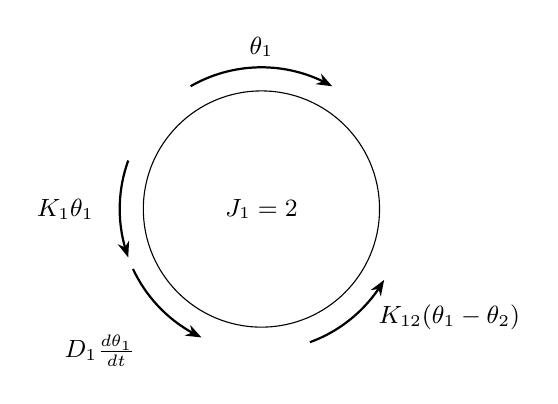
\begin{tikzpicture}[scale=1, every node/.style={font=\small}]
    \node[draw, circle, minimum size=3cm] (j1) {$J_1=2$};
    \draw[-{Stealth[length=2mm]}, thick] (120:1.8cm) arc (120:60:1.8cm) node[midway, above] {$\theta_1$};
    \draw[{Stealth[length=2mm]}-, thick, black] (200:1.8cm) arc(200:160:1.8cm) node[midway, left=2mm]{$K_1\theta_1$};
    \draw[{Stealth[length=2mm]}-, thick, black] (245:1.8cm) arc(245:205:1.8cm) node[midway, below left=2mm]{$D_1\frac{d\theta_1}{dt}$};
    \draw[{Stealth[length=2mm]}-, thick, black] (330:1.8cm) arc(330:290:1.8cm) node[midway, right=2mm]{$K_{12}(\theta_1-\theta_2)$};
  \end{tikzpicture}
\end{figure}

{For ($J_1$):}
\begin{align*}
% sum of torques about $J_1$
J_1\frac{d^2\theta_1}{dt^2}
+ D_1\frac{d\theta_1}{dt}
+ K_1\theta_1
+ K_{12}\!\left(\theta_1-\theta_2\right) &= 0 \\[4pt]
% collect like terms
J_1\frac{d^2\theta_1}{dt^2}
+ D_1\frac{d\theta_1}{dt}
+ (K_1+K_{12})\theta_1
- K_{12}\theta_2 &= 0
\end{align*}

\newpage

{For ($J_2$):}

% ------------ J2 ------------
\begin{figure}[h!]
  \centering
  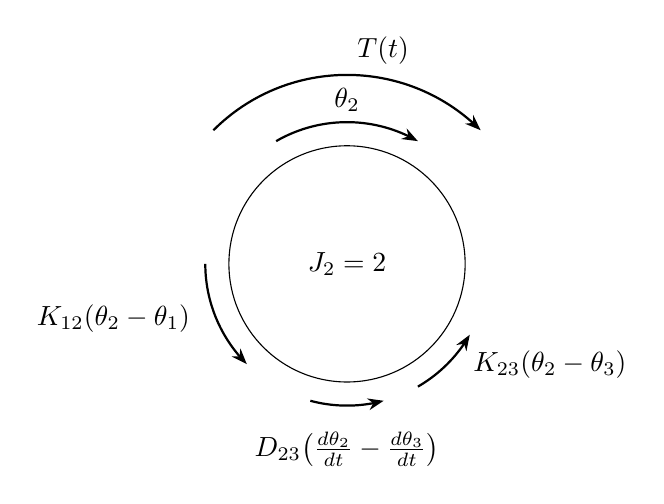
\begin{tikzpicture}[scale=1, every node/.style={font=\normalsize}]
    \node[draw, circle, minimum size=3cm] (j2) {$J_2=2$};
    \draw[-{Stealth[length=2mm]}, thick] (120:1.8cm) arc (120:60:1.8cm) node[midway, above] {$\theta_2$};
    \draw[-{Stealth[length=2mm]}, thick, black!50!black] (135:2.4cm) arc (135:45:2.4cm) node[midway, above right] {$T(t)$};
    \draw[{Stealth[length=2mm]}-, thick, black] (225:1.8cm) arc(225:180:1.8cm) node[midway, left=2mm]{$K_{12}(\theta_2-\theta_1)$};
    \draw[{Stealth[length=2mm]}-, thick, black] (330:1.8cm) arc(330:300:1.8cm) node[midway, right=2mm]{$K_{23}(\theta_2-\theta_3)$};
    \draw[{Stealth[length=2mm]}-, thick, black] (285:1.8cm) arc(285:255:1.8cm) node[midway, below=2mm]{$D_{23}\!\left(\frac{d\theta_2}{dt}-\frac{d\theta_3}{dt}\right)$};
  \end{tikzpicture}
\end{figure}

\begin{align*}
% torque balance from FBD
J_2\frac{d^2\theta_2}{dt^2}
+ D_{23}\!\left(\frac{d\theta_2}{dt}-\frac{d\theta_3}{dt}\right)
+ K_{12}\!\left(\theta_2-\theta_1\right)
+ K_{23}\!\left(\theta_2-\theta_3\right)
- T(t) &= 0 \\[4pt]
% collect terms and move $T(t)$ to RHS
J_2\frac{d^2\theta_2}{dt^2}
+ D_{23}\frac{d\theta_2}{dt}
+ (K_{12}+K_{23})\theta_2
- D_{23}\frac{d\theta_3}{dt}
- K_{12}\theta_1
- K_{23}\theta_3 &= T(t)
\end{align*}

{For ($J_3$):}

% ------------ J3 ------------
\begin{figure}[h!]
  \centering
  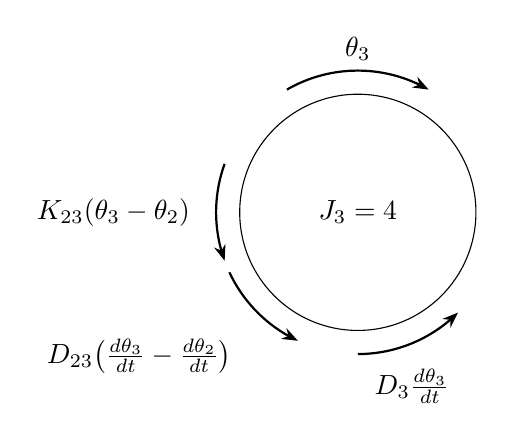
\begin{tikzpicture}[scale=1, every node/.style={font=\normalsize}]
    \node[draw, circle, minimum size=3cm] (j3) {$J_3=4$};
    \draw[-{Stealth[length=2mm]}, thick] (120:1.8cm) arc (120:60:1.8cm) node[midway, above] {$\theta_3$};
    \draw[{Stealth[length=2mm]}-, thick, black] (200:1.8cm) arc(200:160:1.8cm) node[midway, left=2mm]{$K_{23}(\theta_3-\theta_2)$};
    \draw[{Stealth[length=2mm]}-, thick, black] (245:1.8cm) arc(245:205:1.8cm) node[midway, below left=2mm]{$D_{23}\!\left(\frac{d\theta_3}{dt}-\frac{d\theta_2}{dt}\right)$};
    \draw[{Stealth[length=2mm]}-, thick, black] (315:1.8cm) arc(315:270:1.8cm) node[midway, below=2mm]{$D_3\frac{d\theta_3}{dt}$};
  \end{tikzpicture}
\end{figure}


\begin{align*}
% torque balance from FBD
J_3\frac{d^2\theta_3}{dt^2}
+ D_3\frac{d\theta_3}{dt}
+ D_{23}\!\left(\frac{d\theta_3}{dt}-\frac{d\theta_2}{dt}\right)
+ K_{23}\!\left(\theta_3-\theta_2\right) &= 0 \\[4pt]
% collect terms
J_3\frac{d^2\theta_3}{dt^2}
+ (D_3+D_{23})\frac{d\theta_3}{dt}
- D_{23}\frac{d\theta_2}{dt}
+ K_{23}\theta_3
- K_{23}\theta_2 &= 0
\end{align*}


\noindent\textbf{Laplace Transform}
\vspace{8pt}

We take the Laplace transform of the equations, assuming zero initial conditions.
\begin{align}
    (2s^2 + s + 2)\Theta_1(s) - \Theta_2(s) &= 0 \tag{1}\\
    -\Theta_1(s) + (2s^2 + 3s + 4)\Theta_2(s) - (3s+3)\Theta_3(s) &= T(s)\tag{2} \\
    -(3s+3)\Theta_2(s) + (4s^2 + 8s + 3)\Theta_3(s) &= 0 \tag{3}
\end{align}


\noindent\textbf{Solving for the Transfer Function}
\vspace{8pt}

\noindent We use Cramer's rule on the 3x3 system to solve for $\Theta_1(s)$. 

\vspace{8pt}

The transfer function is given by $\dfrac{\Theta_1(s)}{T(s)} = \dfrac{N_1(s)/T(s)}{\Delta(s)}$.

\vspace{8pt}

\noindent\textbf{System Determinant ($\Delta(s)$):}

\vspace{5pt}

The determinant of the system's characteristic matrix is found as follows:
\[
\Delta(s) = \begin{vmatrix} (2s^2+s+2) & -1 & 0 \\ -1 & (2s^2+3s+4) & -(3s+3) \\ 0 & -(3s+3) & (4s^2+8s+3) \end{vmatrix}
\]

Expanding along the first row gives the expression:
\[
\Delta(s) = (2s^2+s+2)\left[(2s^2+3s+4)(4s^2+8s+3) - (3s+3)^2\right] - (-1)\left[(-1)(4s^2+8s+3)\right]
\]

\noindent\textbf{Expanding the Terms:}

\vspace{5pt}

First, we expand the products inside the main bracket:
\begin{align*}
    (2s^2+3s+4)(4s^2+8s+3) &= 8s^4 + 28s^3 + 38s^2 + 41s + 12 \\
    (3s+3)^2 &= 9s^2 + 18s + 9
\end{align*}

Subtracting these gives the value of the main bracket:
\begin{align*}
\text{Bracket Term} &= (8s^4 + 28s^3 + 38s^2 + 41s + 12) - (9s^2 + 18s + 9) \\
&= 8s^4 + 28s^3 + 29s^2 + 23s + 3
\end{align*}

{Final Expansion:}
\vspace{5pt}

Now we substitute this back into the equation for $\Delta(s)$:
\[
\Delta(s) = (2s^2+s+2)(8s^4 + 28s^3 + 29s^2 + 23s + 3) - (4s^2+8s+3)
\]

Completing this final, lengthy multiplication and subtraction yields the result:
\[
\Delta(s) = 16s^6 + 64s^5 + 118s^4 + 139s^3 + 99s^2 + 41s + 3
\]

{Numerator for $\Theta_1$ ($N_1(s)$):}
\[
N_1(s) = \begin{vmatrix} 0 & -1 & 0 \\ T(s) & (2s^2+3s+4) & -(3s+3) \\ 0 & -(3s+3) & (4s^2+8s+3) \end{vmatrix}
\]

Expanding along the first column:
\begin{align*}
    N_1(s) &= -T(s) \cdot \begin{vmatrix} -1 & 0 \\ -(3s+3) & (4s^2+8s+3) \end{vmatrix} \\
    &= -T(s)[(-1)(4s^2+8s+3) - 0] = T(s)(4s^2+8s+3)
\end{align*}

Dividing the numerator by the determinant yields the final result:
\[
\boxed{\frac{\Theta_1(s)}{T(s)} = \frac{4s^2 + 8s + 3}{16s^6 + 64s^5 + 118s^4 + 139s^3 + 99s^2 + 41s + 3}}
\]

% Problem 25 - Rotational Mechanical System Transfer Functions
\newpage
  \setcounter{page}{50}  
\noindent\rule{\textwidth}{1pt}
\noindent\textbf{Problem 25} \hfill 
\\ For the given system, find the transfer function $\frac{\theta_1(s)}{T(s)}$.

\begin{figure}[!ht]
\centering
\resizebox{1\textwidth}{!}{%
\begin{circuitikz}
\tikzstyle{every node}=[font=\LARGE]


\filldraw[pattern=bricks, pattern color=black!60] (-1.75,13.25) rectangle (-1.25,9.75);
\filldraw[pattern=bricks, pattern color=black!60] (19.25,13.25) rectangle (19.75,9.75);

\draw [short] (0.25,12) -- (1.25,12);
\draw [short] (2,12.5) -- (1.25,12.5);
\draw [short] (1.25,12.5) -- (1.25,11.5);
\draw [short] (2.5,12) -- (1.75,12);
\draw [short] (2,11.5) -- (1.25,11.5);
\draw [short] (1.75,12.25) -- (1.75,11.75);
\draw (-1.25,10.75) to[L ] (2.5,10.75);
\draw (-1.25,12) to[L ] (0.25,12);
\draw  (2.5,11.5) ellipse (0.25cm and 1cm);
\draw [short] (2.5,10.5) -- (6.25,10.5);
\draw [short] (2.5,12.5) -- (6.25,12.5);
\draw [short] (6.25,12.5) .. controls (6.75,12.5) and (6.75,10.75) .. (6.25,10.5);
\draw  (11,11.5) ellipse (0.25cm and 1cm);
\draw [short] (11,10.5) -- (14.75,10.5);
\draw [short] (11,12.5) -- (14.75,12.5);
\node [font=\large] at (2,13) {1N-m-s/rad};
\node [font=\large] at (-0.25,12.75) {2N-m/rad};
\node [font=\large] at (0.5,10) {2N-m/rad};
\node [font=\large] at (13.25,11.5) {$2kg-m^2$};
\node [font=\large] at (4.5,11.5) {$4kg-m^2$};
\draw [ color={rgb,255:red,46; green,128; blue,163}, ->, >=Stealth] (5.5,10.25) .. controls (4.75,10.5) and (5,14.5) .. (5.5,12.5) ;
\draw [ color={rgb,255:red,46; green,128; blue,163}, ->, >=Stealth] (4.25,10.25) .. controls (3.5,10.5) and (3.75,14.5) .. (4.25,12.5) ;
\draw [ color={rgb,255:red,46; green,128; blue,163}, ->, >=Stealth] (13.5,10.25) .. controls (12.75,10.5) and (13,14.5) .. (13.5,12.5) ;
\node [font=\large, color={rgb,255:red,46; green,128; blue,163}] at (5.25,13.5) {$\theta_1(t)$};
\node [font=\large, color={rgb,255:red,46; green,128; blue,163}] at (4,13.5) {$T(t)$};
\node [font=\large, color={rgb,255:red,46; green,128; blue,163}] at (13.25,13.5) {$\theta_2(t)$};
\draw [short] (15.1,12) -- (16,12);
\draw [short] (16.75,12.5) -- (16,12.5);
\draw [short] (16,12.5) -- (16,11.5);
\draw [short] (17.25,12) -- (16.5,12);
\draw [short] (16.75,11.5) -- (16,11.5);
\draw [short] (16.5,12.25) -- (16.5,11.75);
\draw (17.25,12) to[L ] (19.25,12);
\node [font=\large] at (16,12.75) {3N-m-s/rad};
\node [font=\large] at (18.25,13) {1N-m/rad};
\node [font=\large] at (16.75,10) {1N-m/rad};
\draw (15,10.75) to[L ] (19.25,10.75);
\draw [short] (6.6,12) -- (7.5,12);
\draw [short] (8.25,12.5) -- (7.5,12.5);
\draw [short] (7.5,12.5) -- (7.5,11.5);
\draw [short] (8.75,12) -- (8,12);
\draw [short] (8.25,11.5) -- (7.5,11.5);
\draw [short] (8,12.25) -- (8,11.75);
\draw (8.75,12) to[L ] (11,12);
\node [font=\large] at (7.5,12.75) {2N-m-s/rad};
\node [font=\large] at (9.75,13) {1N-m/rad};
\draw [short] (6.5,10.75) -- (8.25,10.75);
\draw [short] (9,11.25) -- (8.25,11.25);
\draw [short] (8.25,11.25) -- (8.25,10.25);
\draw [short] (11,10.75) -- (8.75,10.75);
\draw [short] (9,10.25) -- (8.25,10.25);
\draw [short] (8.75,11) -- (8.75,10.5);
\node [font=\large] at (8.75,9.75) {4N-m-s/rad};
\draw [short] (14.75,12.5) .. controls (15.25,12.5) and (15.25,10.75) .. (14.75,10.5);
\end{circuitikz}
}%
\end{figure}

\noindent\rule{\textwidth}{1pt}

\vspace{12pt}


\noindent\textbf{\textit{Given:}}
\[
J_1 = 4\, \text{kg}\cdot\text{m}^2, \quad J_2 = 2\, \text{kg}\cdot\text{m}^2
\]
\[
D_1 = 1\, \text{N}\cdot\text{m}\cdot\text{s/rad}, \quad D_2 = 2\, \text{N}\cdot\text{m}\cdot\text{s/rad}, \quad D_3 = 4\, \text{N}\cdot\text{m}\cdot\text{s/rad}, \quad D_4 = 3\, \text{N}\cdot\text{m}\cdot\text{s/rad}
\]
\[
K_1 = K_2 = 2\, \text{N}\cdot\text{m/rad}, \quad K_3 = K_4 = K_5 = 1\, \text{N}\cdot\text{m/rad}
\]


\vspace{1em}
\noindent

\noindent\textbf{\textit{Required:}}
\[
\frac{\theta_1(s)}{T(s)}
\]

\vspace{1.5em}
\noindent\textbf{\textit{Solution:}}

\vspace{8pt}

\noindent\textbf{Free-Body Diagrams (FBDs)}
\vspace{12pt}

We assume clockwise rotation is positive. The torques shown are the reaction torques opposing

positive motion.

\begin{figure}[h!]
    \centering
    \begin{minipage}{0.48\textwidth}
        \centering
        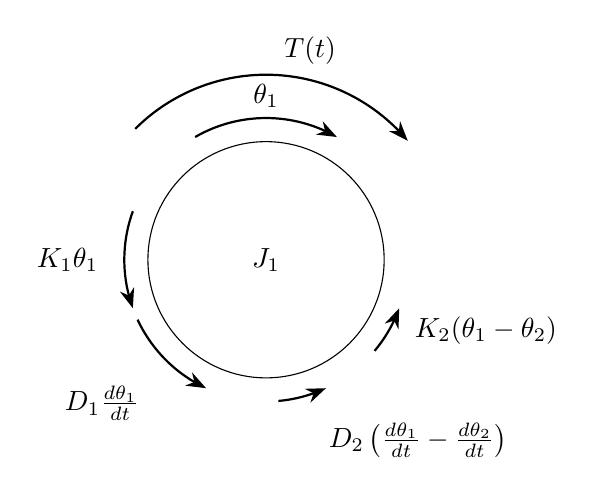
\begin{tikzpicture}[scale=1]
            % J1
            \node[draw, circle, minimum size=3cm] (j1) {$J_1$};
            \draw[-{Stealth[length=2.5mm]}, thick] (120:1.8cm) arc (120:60:1.8cm) node[midway, above] {$\theta_1$};
            \draw[-{Stealth[length=2.5mm]}, thick] (135:2.35cm) arc (135:40:2.35cm) node[midway, above right] {$T(t)$};
            % Wall Torques (CCW)
            \draw[{Stealth[length=2.5mm]}-, thick] (200:1.8cm) arc(200:160:1.8cm) node[midway, left=2mm]{$K_1\theta_1$};
            \draw[{Stealth[length=2.5mm]}-, thick] (245:1.8cm) arc(245:205:1.8cm) node[midway, below left=2mm]{$D_1\frac{d\theta_1}{dt}$};
            % Connecting Torques (CCW)
            \draw[{Stealth[length=2.5mm]}-, thick] (340:1.8cm) arc(340:320:1.8cm) node[midway, right=2mm]{$K_2(\theta_1-\theta_2)$};
            \draw[{Stealth[length=2.5mm]}-, thick] (295:1.8cm) arc(295:275:1.8cm) node[midway, below right=2mm]{$D_2\left(\frac{d\theta_1}{dt}-\frac{d\theta_2}{dt}\right)$};
        \end{tikzpicture}
    \end{minipage}
    \hfill
    \begin{minipage}{0.48\textwidth}
        \centering
        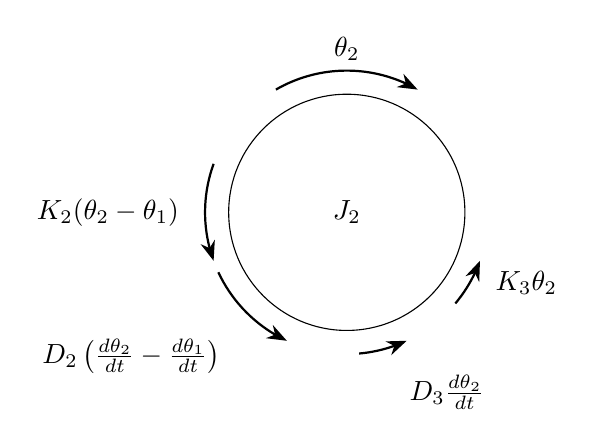
\begin{tikzpicture}[scale=1]
            % J2
            \node[draw, circle, minimum size=3cm] (j2) {$J_2$};
            \draw[-{Stealth[length=2.5mm]}, thick] (120:1.8cm) arc (120:60:1.8cm) node[midway, above] {$\theta_2$};
            % Wall Torques (CCW)
            \draw[{Stealth[length=2.5mm]}-, thick] (340:1.8cm) arc(340:320:1.8cm) node[midway, right=2mm]{$K_3\theta_2$};
            \draw[{Stealth[length=2.5mm]}-, thick] (295:1.8cm) arc(295:275:1.8cm) node[midway, below right=2mm]{$D_3\frac{d\theta_2}{dt}$};
            % Connecting Torques (CCW)
            \draw[{Stealth[length=2.5mm]}-, thick] (200:1.8cm) arc(200:160:1.8cm) node[midway, left=2mm]{$K_2(\theta_2-\theta_1)$};
            \draw[{Stealth[length=2.5mm]}-, thick] (245:1.8cm) arc(245:205:1.8cm) node[midway, below left=2mm]{$D_2\left(\frac{d\theta_2}{dt}-\frac{d\theta_1}{dt}\right)$};
        \end{tikzpicture}
    \end{minipage}
\end{figure}

\noindent\textbf{Equations of Motion}
\vspace{8pt}

\noindent We apply Newton's second law for rotation ($\sum \tau = J \frac{d^2\theta}{dt^2}$) to each inertia.

\vspace{5pt}
{For Inertia 1 ($J_1$):}
\begin{align*}
    J_1 \frac{d^2\theta_1}{dt^2} + D_1 \frac{d\theta_1}{dt} + K_1 \theta_1 + D_2\left(\frac{d\theta_1}{dt} - \frac{d\theta_2}{dt}\right) + K_2(\theta_1 - \theta_2) &= T(t) \\
    J_1 \frac{d^2\theta_1}{dt^2} + (D_1 + D_2)\frac{d\theta_1}{dt} + (K_1 + K_2)\theta_1 - D_2\frac{d\theta_2}{dt} - K_2\theta_2 &= T(t)
\end{align*}

{For Inertia 2 ($J_2$):}
\begin{align*}
    J_2 \frac{d^2\theta_2}{dt^2} + D_3 \frac{d\theta_2}{dt} + K_3 \theta_2 + D_2\left(\frac{d\theta_2}{dt} - \frac{d\theta_1}{dt}\right) + K_2(\theta_2 - \theta_1) &= 0 \\
    J_2 \frac{d^2\theta_2}{dt^2} + (D_2 + D_3)\frac{d\theta_2}{dt} + (K_2 + K_3)\theta_2 - D_2\frac{d\theta_1}{dt} - K_2\theta_1 &= 0
\end{align*}

\newpage
\noindent\textbf{Laplace Transform}
\vspace{12pt}

We take the Laplace transform of the equations, assuming zero initial conditions.
\vspace{5pt}

Equation for Inertia 1:
\[
[J_1 s^2 + (D_1 + D_2)s + (K_1 + K_2)]\Theta_1(s) - [D_2s + K_2]\Theta_2(s) = T(s)
\]

Equation for Inertia 2:
\[
-[D_2s + K_2]\Theta_1(s) + [J_2 s^2 + (D_2 + D_3)s + (K_2 + K_3)]\Theta_2(s) = 0
\]

Substituting the numerical values:
\begin{align}
    (4s^2 + 7s + 5)\Theta_1(s) - (6s + 1)\Theta_2(s) &= T(s) \tag{1} \\
    -(6s + 1)\Theta_1(s) + (2s^2 + 9s + 3)\Theta_2(s) &= 0 \tag{2}
\end{align}

\noindent\textbf{Solving for the Transfer Function}
\vspace{8pt}

The required transfer function is $G(s) = \dfrac{\Theta_1(s)}{T(s)}$. From equation (2), we express $\Theta_2(s)$ in terms

of $\Theta_1(s)$:
\[
\Theta_2(s) = \frac{6s + 1}{2s^2 + 9s + 3} \Theta_1(s)
\]

Substitute this into equation (1):
\[
(4s^2 + 7s + 5)\Theta_1(s) - (6s + 1) \left( \frac{6s + 1}{2s^2 + 9s + 3} \Theta_1(s) \right) = T(s)
\]

Factor out $\Theta_1(s)$:
\[
\left[ \frac{(4s^2 + 7s + 5)(2s^2 + 9s + 3) - (6s + 1)^2}{2s^2 + 9s + 3} \right] \Theta_1(s) = T(s)
\]

Rearrange to find the transfer function $\dfrac{\Theta_1(s)}{T(s)}$:
\[
\frac{\Theta_1(s)}{T(s)} = \frac{2s^2 + 9s + 3}{(4s^2 + 7s + 5)(2s^2 + 9s + 3) - (6s + 1)^2}
\]

Expand and simplify the denominator:
\begin{align*}
    \text{Term 1: } & (4s^2+7s+5)(2s^2+9s+3) = 8s^4 + 50s^3 + 85s^2 + 66s + 15 \\
    \text{Term 2: } & (6s+1)^2 = 36s^2 + 12s + 1 \\
    \text{Denominator} &= (8s^4 + 50s^3 + 85s^2 + 66s + 15) - (36s^2 + 12s + 1) \\
    &= 8s^4 + 50s^3 + 49s^2 + 54s + 14
\end{align*}

The final transfer function is:
\[
\boxed{\frac{\Theta_1(s)}{T(s)} = \frac{2s^2 + 9s + 3}{8s^4 + 50s^3 + 49s^2 + 54s + 14}}
\]


\newpage
% Problem 26 - Transfer Functions involving Gears
  \setcounter{page}{52}  
\noindent\rule{\textwidth}{1pt}
\noindent\textbf{Problem 26} \hfill 
\\ For the given system, find the transfer function $\frac{\theta_2(s)}{T(s)}$.

\begin{figure}[!ht]
\centering
\resizebox{1\textwidth}{!}{%
\begin{circuitikz}
\tikzstyle{every node}=[font=\LARGE]
\filldraw[pattern=bricks, pattern color=black!60] (5.5,9.5) rectangle (7.5,8.75);
\filldraw[pattern=bricks, pattern color=black!60] (20.5,15.5) rectangle (21,9);

\draw [short] (6.75,13.25) -- (6.75,13.25);
\draw [short] (5.5,12.25) -- (7.75,12.25);
\draw (6.5,12.25) to[L ] (6.5,9.5);
\draw (7.75,12.25) ellipse (0.25cm and 0.75cm);
\draw [short] (7.75,13) -- (10.5,13);
\draw [short] (7.75,11.5) -- (10.5,11.5);
\draw [short] (10.5,13) .. controls (11,12.75) and (10.75,11.5) .. (10.5,11.5);
\draw [short] (10.75,12.25) -- (12,12.25);
\draw [short] (12,11.25) -- (12,13.25);
\draw [short] (12,9) -- (12,11);
\draw [short] (12,13.5) -- (12,15.5);
\draw [short] (12,10) -- (13.75,10);
\draw [short] (12,14.5) -- (13.75,14.5);
\draw (13.75,14.5) ellipse (0.25cm and 0.75cm);
\draw [short] (13.75,15.25) -- (16.5,15.25);
\draw [short] (13.75,13.75) -- (16.5,13.75);
\draw [short] (16.5,15.25) .. controls (17,15) and (16.75,13.75) .. (16.5,13.75);
\draw (13.75,10) ellipse (0.25cm and 0.75cm);
\draw [short] (13.75,10.75) -- (16.5,10.75);
\draw [short] (13.75,9.25) -- (16.5,9.25);
\draw [short] (16.5,10.75) .. controls (17,10.5) and (16.75,9.25) .. (16.5,9.25);
\draw [ color={rgb,255:red,46; green,128; blue,163}, ->, >=Stealth] (12.75,9) .. controls (13.5,9) and (13.25,12.5) .. (12.75,10.75) ;
\node [font=\LARGE] at (4.25,11.75) {};
\draw [ color={rgb,255:red,46; green,128; blue,163}, ->, >=Stealth] (6.25,11.25) .. controls (5.5,11.25) and (5.75,14.75) .. (6.25,13) ;
\draw [short] (17.75,15) -- (19,15);
\draw [short] (17.75,14) -- (19,14);
\draw [short] (18.5,14.75) -- (18.5,14.25);
\draw [short] (18.5,14.5) -- (20.5,14.5);
\draw [short] (17.75,15) -- (17.75,14);
\draw [short] (16.75,14.5) -- (17.75,14.5);
\draw (16.75,10) to[L ] (20.5,10);
\node [font=\normalsize] at (18.5,10.75) {300 N-m/rad};
\node [font=\normalsize] at (18.5,15.25) {500 N-m-s/rad};
\node [font=\normalsize] at (7.75,10.75) {3 N-m/rad};
\node [font=\normalsize] at (15.25,10) {$150 kg-m^2$};
\node [font=\normalsize] at (9.25,12.25) {$3 kg-m^2$};
\node [font=\normalsize] at (15.25,14.5) {$100 kg-m^2$};
\node [font=\normalsize] at (11.25,10) {$N_2 = 50$};
\node [font=\normalsize] at (11.25,14.5) {$N_3 = 25$};
\node [font=\normalsize, color={rgb,255:red,46; green,128; blue,163}] at (6,13.75) {$T(t)$};
\node [font=\normalsize, color={rgb,255:red,46; green,128; blue,163}] at (13,11.5) {$\theta_2 (t)$};
\node [font=\normalsize] at (12.75,12.25) {$N_1 = 5$};
\end{circuitikz}
}%
\end{figure}

\noindent\rule{\textwidth}{1pt}

\vspace{12pt}


\noindent\textbf{\textit{Given:}}
\[
J_1 = 3 \text{kg-m}^2, J_2 = 150 \text{kg-m}^2, J_3 = 100 \text{kg-m}^2
\]
\[
K_1 = 3 \text{N-m/rad}, K_2 = 300 \text{N-m/rad}
\]
\[
D_3 = 500 \text{N-m-s/rad}
\]
\[
  N_1 = 5, N_2 = 50, N_3 = 25
\]
\vspace{1em}
\noindent

\noindent\textbf{\textit{Required:}}
\[
\frac{\theta_2(s)}{T(s)}
\]

\vspace{1.5em}
\noindent\textbf{\textit{Solution:}}



\begin{figure}[!ht]
\centering
\resizebox{0.9\textwidth}{!}{%
\begin{circuitikz}
\tikzstyle{every node}=[font=\LARGE]


\filldraw[pattern=bricks, pattern color=black!60] (5.5,2.25) rectangle (7.5,1.5);
\filldraw[pattern=bricks, pattern color=black!60] (20,6.75) rectangle (20.5,2);

\draw [short] (6.75,6) -- (6.75,6);
\draw [short] (5.5,5) -- (7.75,5);
\draw (6.5,5) to[L ] (6.5,2.25);
\draw (7.75,5) ellipse (0.25cm and 0.75cm);
\draw [short] (7.75,5.75) -- (10.5,5.75);
\draw [short] (7.75,4.25) -- (10.5,4.25);
\draw [short] (10.5,5.75) .. controls (11,5.5) and (10.75,4.25) .. (10.5,4.25);
\draw [short] (10.75,5) -- (11.5,5);
\draw [short] (11.5,3) -- (11.5,5);
\draw [short] (11.5,3) -- (13.25,3);
\draw [short] (11.5,5) -- (13.25,5);
\draw (13.25,5) ellipse (0.25cm and 0.75cm);
\draw [short] (13.25,5.75) -- (16,5.75);
\draw [short] (13.25,4.25) -- (16,4.25);
\draw [short] (16,5.75) .. controls (16.5,5.5) and (16.25,4.25) .. (16,4.25);
\draw (13.25,3) ellipse (0.25cm and 0.75cm);
\draw [short] (13.25,3.75) -- (16,3.75);
\draw [short] (13.25,2.25) -- (16,2.25);
\draw [short] (16,3.75) .. controls (16.5,3.5) and (16.25,2.25) .. (16,2.25);
\node [font=\LARGE] at (4.25,4.25) {};
\draw [ color={rgb,255:red,46; green,128; blue,163}, ->, >=Stealth] (6.25,4) .. controls (5.5,4) and (5.75,7.5) .. (6.25,5.75) ;
\draw [short] (17.25,5.5) -- (18.5,5.5);
\draw [short] (17.25,4.5) -- (18.5,4.5);
\draw [short] (18,5.25) -- (18,4.75);
\draw [short] (18,5) -- (20,5);
\draw [short] (17.25,5.5) -- (17.25,4.5);
\draw [short] (16.25,5) -- (17.25,5);
\draw (16.25,3) to[L ] (20,3);
\node [font=\normalsize] at (7.75,3.5) {3 N-m/rad};
\node [font=\normalsize] at (9.25,5) {$3 kg-m^2$};
\node [font=\normalsize, color={rgb,255:red,46; green,128; blue,163}] at (6,6.5) {$T(t)$};
\node [font=\normalsize] at (14.75,6.25) {$100 \left(\frac{5}{25}\right)^2$
};
\node [font=\normalsize] at (18,6.25) {$500 \left(\frac{5}{25}\right)^2$

};
\node [font=\normalsize] at (18,2.25) {$300 \left(\frac{5}{50}\right)^2$

};
\node [font=\normalsize] at (15,1.75) {$150 \left(\frac{5}{25}\right)^2$

};
\end{circuitikz}
}%
\end{figure}


\vspace{8pt}

{Component Reflection to Input Shaft (Shaft 1)}

\vspace{10pt}

{Reflecting Shaft 2 to Shaft 1:}
\begin{align*}
 J_{2,eq} &= J_2\left(\frac{N_1}{N_2}\right)^2 = 150\left(\frac{5}{50}\right)^2 = 1.5 \, \text{kg-m}^2 \\
 K_{2,eq} &= K_2\left(\frac{N_1}{N_2}\right)^2 = 300\left(\frac{5}{50}\right)^2 = 3 \, \text{N-m/rad}
\end{align*}

{Reflecting Shaft 3 to Shaft 1:}
\begin{align*}
 J_{3,eq} &= J_3\left(\frac{N_1}{N_3}\right)^2 = 100\left(\frac{5}{25}\right)^2 = 4 \, \text{kg-m}^2 \\
 D_{3,eq} &= D_3\left(\frac{N_1}{N_3}\right)^2 = 500\left(\frac{5}{25}\right)^2 = 20 \, \text{N-m-s/rad}
\end{align*}

\vspace{10pt}

\newpage
\noindent\textbf{Equation of Motion}
\vspace{5pt}

$\sum M=0 \quad (\circlearrowright +)$
\begin{align*}
    & T(s) - (J_1 + J_{2,eq} + J_{3,eq})s^2\theta_1(s) - (D_1 + D_2 + D_{3,eq})s\theta_1(s) - (K_1 + K_{2,eq} + K_3)\theta_1(s) = 0 \\
    & T(s) - (3 + 1.5 + 4)s^2\theta_1(s) - (0 + 0 + 20)s\theta_1(s) - (3 + 3 + 0)\theta_1(s) = 0 \\
    & T(s) - 8.5s^2\theta_1(s) - 20s\theta_1(s) - 6\theta_1(s) = 0
\end{align*}

\vspace{10pt}

\noindent\textbf{Transfer Function}
\begin{equation*}
 (8.5s^2 + 20s + 6)\theta_1(s) = T(s)
\end{equation*}

The relationship between the output angle $\theta_2(s)$ and the input angle $\theta_1(s)$ is:
\begin{equation*}
    \frac{\theta_2(s)}{\theta_1(s)} = \frac{N_1}{N_2} = \frac{5}{50} = \frac{1}{10}
\end{equation*}

Combining the equations to find the final transfer function:
\begin{equation*}
 \frac{\theta_2(s)}{T(s)} = \frac{\theta_2(s)}{\theta_1(s)} \times \frac{\theta_1(s)}{T(s)} = \frac{1}{10} \left( \frac{1}{8.5s^2 + 20s + 6} \right)
\end{equation*}
\begin{equation*}
 \boxed{
 \frac{\theta_2(s)}{T(s)} = \frac{1}{85s^2 + 200s + 60}
 }
\end{equation*}



% Problem 27 - Transfer Functions involving Gears

\newpage
  \setcounter{page}{54}  
\noindent\rule{\textwidth}{1pt}
\noindent\textbf{Problem 27} \hfill 
\\ For the given system, find the transfer function $\frac{\theta_1(s)}{T(s)}$.

\begin{figure}[!ht]
\centering
\resizebox{0.9\textwidth}{!}{%
\begin{circuitikz}
\tikzstyle{every node}=[font=\large]


\filldraw[pattern=bricks, pattern color=black!60] (-1,9.5) rectangle (0.75,8.75);
\filldraw[pattern=bricks, pattern color=black!60] (17.75,17.25) rectangle (18.5,9);

\node [font=\large] at (15,8.75) {1N-m-s/rad};
\node [font=\large] at (1.5,11.25) {2N-m/rad};
\draw [ color={rgb,255:red,46; green,128; blue,163}, ->, >=Stealth] (-0.5,12) .. controls (-1.25,12.25) and (-1,16.25) .. (-0.5,14.25) ;
\node [font=\large, color={rgb,255:red,46; green,128; blue,163}] at (-0.75,15.25) {$T(t)$};
\node [font=\large] at (16.25,16.75) {2 N-m/rad};
\node [font=\large] at (14,14.75) {300 N-m-s/rad};
\node [font=\large] at (15,12) {400N-m/rad};
\draw (-0.25,13.25) to[L ] (-0.25,9.5);
\draw [short] (-1.25,13.25) -- (0.75,13.25);
\draw  (1,13.25) ellipse (0.25cm and 1cm);
\node [font=\LARGE] at (5.25,13.25) {};
\node [font=\LARGE] at (3,12.25) {};
\draw [short] (1,14.25) -- (4.75,14.25);
\draw [short] (1,12.25) -- (4.75,12.25);
\draw [short] (4.75,14.25) .. controls (5.25,13.75) and (5,12.5) .. (4.75,12.25);
\draw [short] (5,13.25) -- (6.75,13.25);
\draw [short] (6.75,14.5) -- (6.75,12);
\draw [short] (6.75,17.25) -- (6.75,14.75);
\draw [short] (6.75,16) -- (8.5,16);
\draw [short] (8.5,17) -- (12.25,17);
\draw  (8.5,16) ellipse (0.25cm and 1cm);
\draw [short] (8.5,15) -- (12.25,15);
\draw [short] (12.25,17) .. controls (12.75,16.5) and (12.5,15.25) .. (12.25,15);
\draw [short] (8.5,11.5) -- (12.25,11.5);
\draw  (8.5,10.5) ellipse (0.25cm and 1cm);
\draw [short] (8.5,9.5) -- (12.25,9.5);
\draw [short] (12.25,11.5) .. controls (12.75,11) and (12.5,9.75) .. (12.25,9.5);
\draw [short] (6.75,11.75) -- (6.75,9.25);
\draw [short] (6.75,10.5) -- (8.5,10.5);
\draw [short] (12.5,16) -- (13.75,16);
\draw [short] (14.5,16.5) -- (13.75,16.5);
\draw [short] (13.75,16.5) -- (13.75,15.5);
\draw [short] (15,16) -- (14.25,16);
\draw [short] (14.5,15.5) -- (13.75,15.5);
\draw [short] (14.25,16.25) -- (14.25,15.75);
\draw (12.5,11) to[L ] (17.75,11);
\draw [short] (12.5,10) -- (14.75,10);
\draw [short] (15.5,10.5) -- (14.75,10.5);
\draw [short] (14.75,10.5) -- (14.75,9.5);
\draw [short] (17.75,10) -- (15.25,10);
\draw [short] (15.5,9.5) -- (14.75,9.5);
\draw [short] (15.25,10.25) -- (15.25,9.75);
\draw (15,16) to[L ] (17.75,16);
\node [font=\large] at (3,13.25) {$2kg-m^2$};
\node [font=\large] at (10.5,16) {$100kg-m^2$};
\node [font=\large] at (10.5,10.5) {$150kg-m^2$};
\draw [ color={rgb,255:red,46; green,128; blue,163}, ->, >=Stealth] (7.25,14.5) .. controls (8,14.75) and (8,18.75) .. (7.25,16.75) ;
\node [font=\large, color={rgb,255:red,46; green,128; blue,163}] at (7.75,17.75) {$\theta_1(t)$};
\node [font=\large] at (5.75,16) {$N_3 = 25$};
\node [font=\large] at (5.75,10.5) {$N_2 = 50$};
\node [font=\large] at (7.75,13.25) {$N_1 = 5$};
\end{circuitikz}
}%
\end{figure}

\noindent\rule{\textwidth}{1pt}

\vspace{12pt}


\noindent\textbf{\textit{Given:}}
\[
J_1 = 2\,\text{kg} \cdot \text{m}^2, \quad J_2 = 150\,\text{kg} \cdot \text{m}^2, \quad J_3 = 100\,\text{kg} \cdot \text{m}^2
\]
\[
K_1,K_2 = 2\,\text{N} \cdot \text{m/rad}, \quad K_3 = 400\,\text{N} \cdot \text{m/rad}
\]
\[
D_1 = 300\,\text{N} \cdot \text{m} \cdot \text{s/rad}, \quad D_2 = D_3 = 1\,\text{N} \cdot \text{m} \cdot \text{s/rad}
\]
\[
N_1 = 5, \quad N_2 = 50, \quad N_3 = 25
\]



\vspace{1em}
\noindent

\noindent\textbf{\textit{Required:}}
\[
\frac{\theta_1(s)}{T(s)}
\]

\vspace{1.5em}
\noindent\textbf{\textit{Solution:}}

\vspace{8pt}

\begin{figure}[!ht]
\centering
\resizebox{0.9\textwidth}{!}{%
\begin{circuitikz}
\tikzstyle{every node}=[font=\large]


\filldraw [pattern=bricks, pattern color=black!60] (-1,9.75) rectangle (0.75,9);
\filldraw [pattern=bricks, pattern color=black!60] (17,15.5) rectangle (17.75,8.75);

\draw (-0.25,13.5) to[L ] (-0.25,9.75);
\draw [short] (-1.25,13.5) -- (0.75,13.5);
\node [font=\LARGE] at (1,13.5) {};
\draw [short] (1,14.5) -- (4.75,14.5);
\draw [short] (4.75,14.5) .. controls (5.25,14) and (5,12.75) .. (4.75,12.5);
\draw [short] (1,12.5) -- (4.75,12.5);
\node [font=\large] at (3,13.5) {$2kg-m^2$};
\draw  (1,13.5) ellipse (0.25cm and 1cm);
\draw [short] (5,13.5) -- (7.5,13.5);
\draw [short] (7.75,12.5) -- (11.5,12.5);
\draw [short] (11.5,14.5) .. controls (12,14) and (11.75,12.75) .. (11.5,12.5);
\draw [short] (7.75,14.5) -- (11.5,14.5);
\draw  (7.75,13.5) ellipse (0.25cm and 1cm);
\draw [short] (5.75,13.5) -- (5.75,10.75);
\draw [short] (5.75,10.75) -- (7.75,10.75);
\draw [short] (7.75,9.75) -- (11.5,9.75);
\draw [short] (11.5,11.75) .. controls (12,11.25) and (11.75,10) .. (11.5,9.75);
\draw [short] (7.75,11.75) -- (11.5,11.75);
\draw  (7.75,10.75) ellipse (0.25cm and 1cm);
\draw [short] (11.75,10.25) -- (14,10.25);
\draw [short] (14.75,10.75) -- (14,10.75);
\draw [short] (14,10.75) -- (14,9.75);
\draw [short] (17,10.25) -- (14.5,10.25);
\draw [short] (14.5,10.5) -- (14.5,10);
\draw (11.75,11.25) to[L ] (17,11.25);
\draw [short] (14.75,9.75) -- (14,9.75);
\node [font=\large] at (15.5,14.25) {$2(5/25)^2$};
\draw [short] (11.75,13.5) -- (13,13.5);
\draw [short] (13.75,14) -- (13,14);
\draw [short] (13,14) -- (13,13);
\draw [short] (14.25,13.5) -- (13.5,13.5);
\draw [short] (13.75,13) -- (13,13);
\draw [short] (13.5,13.75) -- (13.5,13.25);
\draw (14.25,13.5) to[L ] (17,13.5);
\node [font=\large] at (1.25,11.5) {2N-m/rad};
\node [font=\large] at (9.75,15) {$100(5/25)^2$};
\node [font=\large] at (9.75,9) {$150(5/50)^2$};
\node [font=\large] at (13.25,14.75) {$300(5/25)^2$};
\node [font=\large] at (14.5,12) {$400(5/50)^2$};
\node [font=\large] at (14.5,9.25) {$1(5/50)^2$};
\end{circuitikz}
}%
\end{figure}


\vspace{8pt}


\noindent\textbf{Component Reflection to Input Shaft (Shaft 1)}
\vspace{5pt}

{Reflecting Shaft 2 to Shaft 1:}
\begin{align*}
    J_{2,eq} &= J_2\left(\frac{N_1}{N_2}\right)^2 = 150\left(\frac{5}{50}\right)^2 = 1.5 \, \text{kg-m}^2 \\
    D_{2,eq} &= D_2\left(\frac{N_1}{N_2}\right)^2 = 1\left(\frac{5}{50}\right)^2 = 0.01 \, \text{N-m-s/rad} \\
    K_{2,eq} &= K_2\left(\frac{N_1}{N_2}\right)^2 = 400\left(\frac{5}{50}\right)^2 = 4 \, \text{N-m/rad}
\end{align*}
\vspace{10pt}

{Reflecting Shaft 3 to Shaft 1:}
\begin{align*}
    J_{3,eq} &= J_3\left(\frac{N_1}{N_3}\right)^2 = 100\left(\frac{5}{25}\right)^2 = 4 \, \text{kg-m}^2 \\
    D_{3,eq} &= D_3\left(\frac{N_1}{N_3}\right)^2 = 300\left(\frac{5}{25}\right)^2 = 12 \, \text{N-m-s/rad} \\
    K_{3,eq} &= K_3\left(\frac{N_1}{N_3}\right)^2 = 2\left(\frac{5}{25}\right)^2 = 0.08 \, \text{N-m/rad}
\end{align*}

\noindent\textbf{Equation of Motion}
\vspace{5pt}

\[
\sum M = 0 \quad (\circlearrowright +)
\]
\begin{align*}
    & T(s) - (J_1 + J_{2,eq} + J_{3,eq})s^2\theta_{in}(s) - (D_{2,eq} + D_{3,eq})s\theta_{in}(s) - (K_1 + K_{2,eq} + K_{3,eq})\theta_{in}(s) = 0 \\
    & T(s) - (2 + 1.5 + 4)s^2\theta_{in}(s) - (0.01 + 12)s\theta_{in}(s) - (2 + 4 + 0.08)\theta_{in}(s) = 0 \\
    & T(s) - 7.5s^2\theta_{in}(s) - 12.01s\theta_{in}(s) - 6.08\theta_{in}(s) = 0
\end{align*}

\vspace{10pt} 

\noindent\textbf{Transfer Function}
\begin{equation*}
 (7.5s^2 + 12.01s + 6.08)\theta_{in}(s) = T(s)
\end{equation*}

The relationship between the output angle $\theta_1(s)$ and the equivalent input angle $\theta_{in}(s)$ is:
\begin{equation*}
    \frac{\theta_1(s)}{\theta_{in}(s)} = \frac{N_1}{N_3} = \frac{5}{25} = \frac{1}{5}
\end{equation*}

Combining the equations to find the final transfer function:
\begin{equation*}
 \frac{\theta_1(s)}{T(s)} = \frac{\theta_1(s)}{\theta_{in}(s)} \times \frac{\theta_{in}(s)}{T(s)} = \frac{1}{5} \left( \frac{1}{7.5s^2 + 12.01s + 6.08} \right)
\end{equation*}
\begin{equation*}
 \boxed{
 \frac{\theta_1(s)}{T(s)} = \frac{1}{37.5s^2 + 60.05s + 30.4}
 }
\end{equation*}



% Problem 28 - Transfer Functions involving Gears

\newpage
  \setcounter{page}{56}  
\noindent\rule{\textwidth}{1pt}
\noindent\textbf{Problem 28} \hfill 
\\ For the given system, find the transfer function $\frac{\theta_1(s)}{T(s)}$.

\begin{figure}[!ht]
\centering
\resizebox{0.8\textwidth}{!}{%
\begin{circuitikz}
\tikzstyle{every node}=[font=\normalsize]


\filldraw[pattern=bricks, pattern color=black!60] (23.75,2) rectangle (24.25,-0.5);


\draw [short] (6.5,6.25) -- (6.5,6.25);
\draw [short] (5.25,5.25) -- (7.5,5.25);
\draw (7.5,5.25) ellipse (0.25cm and 0.75cm);
\draw [short] (7.5,6) -- (9.75,6);
\draw [short] (7.5,4.5) -- (9.75,4.5);
\draw [short] (9.75,6) .. controls (10.25,5.75) and (10,4.5) .. (9.75,4.5);
\draw [ color={rgb,255:red,46; green,128; blue,163}, ->, >=Stealth] (6,4.25) .. controls (5.25,4.25) and (5.5,7.75) .. (6,6) ;
\node [font=\normalsize] at (8.75,5.25) {$J_a$};
\node [font=\normalsize, color={rgb,255:red,46; green,128; blue,163}] at (5.75,6.75) {$T(t)$};
\draw [short] (11.25,4.25) -- (11.25,6.25);
\draw [short] (10,5.25) -- (11.25,5.25);
\node [font=\normalsize] at (12,6) {$N_1 $};
\node [font=\normalsize] at (12,4.5) {$J_1 $};
\draw [short] (11.25,2) -- (11.25,4);
\node [font=\normalsize] at (10.5,3.75) {$N_2$};
\node [font=\normalsize] at (10.5,2.25) {$J_2 $};
\draw (11.25,3) to[L ] (13.75,3);
\draw [short] (13.75,3.5) -- (15,3.5);
\draw [short] (14.5,3.25) -- (14.5,2.75);
\draw [short] (14.5,3) -- (15.75,3);
\draw [short] (13.75,3.5) -- (13.75,2.5);
\node [font=\normalsize] at (16.5,3.75) {$N_3 $};
\node [font=\normalsize] at (16.5,2.25) {$J_3 $};
\draw [short] (15.75,2) -- (15.75,4);
\draw [short] (17,4) -- (17,4);
\node [font=\normalsize] at (15,1.5) {$N_4$};
\draw [short] (15.75,-0.25) -- (15.75,1.75);
\node [font=\normalsize] at (15,0) {$J_4$};
\draw [short] (15.75,0.75) -- (18,0.75);
\draw (18,0.75) ellipse (0.25cm and 0.75cm);
\draw [short] (18,1.5) -- (20.25,1.5);
\draw [short] (18,0) -- (20.25,0);
\draw [short] (20.25,1.5) .. controls (20.75,1.25) and (20.5,0) .. (20.25,0);
\node [font=\normalsize] at (19.25,0.75) {$J_L$};
\draw [short] (20.5,0.75) -- (21.75,0.75);
\draw [short] (21.75,1.25) -- (23,1.25);
\draw [short] (13.75,2.5) -- (15,2.5);
\draw [short] (22.5,1) -- (22.5,0.5);
\draw [short] (22.5,0.75) -- (23.75,0.75);
\draw [short] (21.75,1.25) -- (21.75,0.25);
\draw [short] (21.75,0.25) -- (23,0.25);
\node [font=\normalsize, color={rgb,255:red,46; green,128; blue,163}] at (6.5,6.75) {$\theta_1(t)$};
\draw [ color={rgb,255:red,46; green,128; blue,163}, ->, >=Stealth] (6.75,4.25) .. controls (6,4.25) and (6.25,7.75) .. (6.75,6) ;
\node [font=\normalsize] at (14.5,4) {$D$};
\node [font=\normalsize] at (12.5,3.75) {$K$};
\node [font=\normalsize] at (22.5,1.75) {$D_L$};
\end{circuitikz}
}%
\end{figure}

\noindent\rule{\textwidth}{1pt}

\vspace{12pt}


\noindent\textbf{\textit{Given:}}
\[
\text{Inertias:} \quad J_a, \quad J_2, \quad J_3, \quad J_L
\]
\[
\text{Stiffnesses:} \quad K_1, \quad K_2
\]
\[
\text{Dampings:} \quad D, \quad D_L
\]
\[
\text{Gear Ratios:} \quad N_1, \quad N_2, \quad N_3, \quad N_4
\]

\vspace{1em}
\noindent

\noindent\textbf{\textit{Required:}}
\[
\frac{\theta_1(s)}{T(s)}
\]

\vspace{1.5em}
\noindent\textbf{\textit{Solution:}}



\begin{figure}[!ht]
\centering
\resizebox{1\textwidth}{!}{%
\begin{circuitikz}
\tikzstyle{every node}=[font=\normalsize]


\filldraw[pattern=bricks, pattern color=black!60] (24,-3) rectangle (24.5,-5.5);


\draw [short] (5.25,-3.25) -- (5.25,-3.25);
\draw [short] (4,-4.25) -- (6.25,-4.25);
\draw (6.25,-4.25) ellipse (0.25cm and 0.75cm);
\draw [short] (6.25,-3.5) -- (8.5,-3.5);
\draw [short] (6.25,-5) -- (8.5,-5);
\draw [short] (8.5,-3.5) .. controls (9,-3.75) and (8.75,-5) .. (8.5,-5);
\draw [ color={rgb,255:red,46; green,128; blue,163}, ->, >=Stealth] (4.75,-5.25) .. controls (4,-5.25) and (4.25,-1.75) .. (4.75,-3.5) ;
\node [font=\normalsize] at (7.5,-4.25) {$J_a + J_1$};
\node [font=\normalsize, color={rgb,255:red,46; green,128; blue,163}] at (4.5,-2.75) {$T(t)$};
\draw [short] (8.75,-4.25) -- (10,-4.25);
\node [font=\normalsize, color={rgb,255:red,46; green,128; blue,163}] at (5.25,-2.75) {$\theta_1(t)$};
\draw [ color={rgb,255:red,46; green,128; blue,163}, ->, >=Stealth] (5.5,-5.25) .. controls (4.75,-5.25) and (5,-1.75) .. (5.5,-3.5) ;
\draw (10.25,-4.25) ellipse (0.25cm and 0.75cm);
\draw [short] (10.25,-3.5) -- (13,-3.5);
\draw [short] (10.25,-5) -- (13,-5);
\draw [short] (13,-3.5) .. controls (13.5,-3.75) and (13.25,-5) .. (13,-5);
\node [font=\normalsize] at (12,-4.25) {$J_2 + J_3 \left(\frac{N_1}{N_2}\right)^2$};
\draw (13.25,-4.25) to[L ] (15.75,-4.25);
\node [font=\LARGE] at (15.75,-4.25) {};
\draw [short] (15.75,-3.75) -- (17,-3.75);
\draw [short] (16.5,-4) -- (16.5,-4.5);
\draw [short] (16.5,-4.25) -- (17.75,-4.25);
\draw [short] (15.75,-3.75) -- (15.75,-4.75);
\draw [short] (15.75,-4.75) -- (17,-4.75);
\node [font=\LARGE] at (16.25,-4.75) {};
\draw (17.75,-4.25) ellipse (0.25cm and 0.75cm);
\draw [short] (17.75,-3.5) -- (20.5,-3.5);
\draw [short] (17.75,-5) -- (20.5,-5);
\draw [short] (20.5,-3.5) .. controls (21,-3.75) and (20.75,-5) .. (20.5,-5);
\draw [short] (20.75,-4.25) -- (22,-4.25);
\draw [short] (22,-3.75) -- (23.25,-3.75);
\draw [short] (22.75,-4) -- (22.75,-4.5);
\draw [short] (22.75,-4.25) -- (24,-4.25);
\draw [short] (22,-3.75) -- (22,-4.75);
\draw [short] (22,-4.75) -- (23.25,-4.75);
\node [font=\normalsize] at (22.75,-3.25) {$D_L \left(\frac{N_3 N_1}{N_4 N_2}\right)^2$};
\node [font=\LARGE] at (22.5,-4.75) {};
\node [font=\normalsize] at (14.75,-3.5) {$K \left(\frac{N_1}{N_2}\right)^2$};
\node [font=\normalsize] at (16.75,-3.2) {$D \left(\frac{N_1}{N_2}\right)^2$};
\node [font=\small] at (19.4,-4.25) {$J_4 + J_L \left(\frac{N_3 N_1}{N_4 N_2}\right)^2$};
\end{circuitikz}
}%
\end{figure}

\vspace{8pt}





\noindent\textbf{System Equations and Transfer Function}

\vspace{5pt}

\[
\sum M = 0 \quad (\circlearrowright +) \quad 
\]


\begin{center}
\resizebox{0.94\textwidth}{!}{$
T(s) - \left[ J_a + J_1 + (J_2 + J_x) \left( \frac{N_1}{N_2} \right)^2 + (J_y + J_L) \left( \frac{N_3 N_1}{N_4 N_2} \right)^2 \right] s^2 \Theta_1(s)
- D_L \left( \frac{N_3 N_1}{N_4 N_2} \right)^2 s \Theta_1(s)
- K \left( \frac{N_1}{N_2} \right)^2 \Theta_1(s) = 0
$}
\end{center}


\begin{center}
\resizebox{0.94\textwidth}{!}{$
T(s) = \Theta_1(s) \left\{
\left[ J_a + J_1 + (J_2 + J_x) \left( \frac{N_1}{N_2} \right)^2 + (J_y + J_L) \left( \frac{N_3 N_1}{N_4 N_2} \right)^2 \right] s^2
+ D_L \left( \frac{N_3 N_1}{N_4 N_2} \right)^2 s
+ K \left( \frac{N_1}{N_2} \right)^2
\right\}
$}
\end{center}


{Rearranging to solve for the transfer function } G(s):

\begin{center}
\fbox{%
\begin{minipage}{0.94\textwidth}
\begin{equation*}
\frac{\Theta_1(s)}{T(s)} =
\frac{1}{
\left[ J_a + J_1 + (J_2 + J_x) \left( \frac{N_1}{N_2} \right)^2 + (J_y + J_L) \left( \frac{N_3 N_1}{N_4 N_2} \right)^2 \right] s^2
+ D_L \left( \frac{N_3 N_1}{N_4 N_2} \right)^2 s
+ K \left( \frac{N_1}{N_2} \right)^2
}
\end{equation*}
\end{minipage}
}
\end{center}




% Problem 29 - Transfer Functions involving Gears

\newpage
  \setcounter{page}{57}  
\noindent\rule{\textwidth}{1pt}
\noindent\textbf{Problem 29} \hfill 
\\ For the given system, find the transfer function $\frac{\theta_2(s)}{T(s)}$.

\begin{figure}[!ht]
\centering
\resizebox{0.8\textwidth}{!}{%
\begin{circuitikz}
\tikzstyle{every node}=[font=\LARGE]


\filldraw[pattern=bricks, pattern color=black!60] (22.5,2) rectangle (23,-0.5);


\draw [short] (6.75,6) -- (6.75,6);
\draw [short] (5.5,5) -- (7.75,5);
\draw (7.5,5.25) ellipse (0.25cm and 0.75cm);
\draw [short] (7.5,6) -- (9.75,6);
\draw [short] (7.5,4.5) -- (9.75,4.5);
\draw [short] (9.75,6) .. controls (10.25,5.75) and (10,4.5) .. (9.75,4.5);
\draw [ color={rgb,255:red,46; green,128; blue,163}, ->, >=Stealth] (7.25,4.25) .. controls (6.5,4.25) and (6.75,7.75) .. (7.25,6) ;
\node [font=\normalsize, color={rgb,255:red,46; green,128; blue,163}] at (7,6.75) {$T(t)$};
\draw [short] (11.25,4.25) -- (11.25,6.25);
\draw [short] (10,5.25) -- (11.25,5.25);
\node [font=\normalsize] at (12,6) {$N_1 =4$};
\node [font=\normalsize] at (13.2,4.5) {$D_1 = 1 N-m-s/rad $};
\draw [short] (11.25,2) -- (11.25,4);
\node [font=\normalsize] at (10.5,3.75) {$N_2 = 12$};
\node [font=\normalsize] at (9.25,2.25) {$D_2 = 2 N-m-s/rad $};
\node [font=\normalsize] at (16.5,3.75) {$N_3 = 4 $};
\draw [short] (15.75,2) -- (15.75,4);
\draw [short] (17,4) -- (17,4);
\node [font=\normalsize] at (15,1.5) {$N_4 = 16$};
\draw [short] (15.75,-0.25) -- (15.75,1.75);
\node [font=\normalsize] at (13.5,0) {$D_3 = 32 N-m-s/rad$};
\draw [short] (15.75,0.75) -- (17,0.75);
\draw (17.25,0.75) ellipse (0.25cm and 0.75cm);
\draw [short] (17.25,1.5) -- (19.5,1.5);
\draw [short] (17.25,0) -- (19.5,0);
\draw [short] (19.5,1.5) .. controls (20,1.25) and (19.75,0) .. (19.5,0);
\node [font=\normalsize] at (18.5,0.75) {$16kg-m^2$};
\draw [ color={rgb,255:red,46; green,128; blue,163}, ->, >=Stealth] (11.5,1.75) .. controls (12.25,1.75) and (12.25,5.25) .. (11.5,3.5) ;
\node [font=\normalsize, color={rgb,255:red,46; green,128; blue,163}] at (12.5,4) {$\theta_2(t)$};
\draw [short] (11.25,3) -- (12.25,3);
\draw (12.25,3) ellipse (0.25cm and 0.75cm);
\draw [short] (12.25,3.75) -- (14.5,3.75);
\draw [short] (12.25,2.25) -- (14.5,2.25);
\draw [short] (14.5,3.75) .. controls (15,3.5) and (14.75,2.25) .. (14.5,2.25);
\draw [short] (14.75,3) -- (15.75,3);
\draw (19.75,0.75) to[L ] (22.5,0.75);
\node [font=\normalsize] at (21.25,1.25) {$64 N-m/rad $};
\node [font=\normalsize] at (13.5,3) {$1kg-m^2$};
\node [font=\normalsize] at (8.75,5.25) {$1kg-m^2$};
\end{circuitikz}
}%
\end{figure}
\vspace{-1em}

\noindent\rule{\textwidth}{1pt}

\vspace{12pt}


\noindent\textbf{\textit{Given:}}
\[
\text{Inertias:} \quad J_a = 1\,\text{kg}\cdot\text{m}^2, \quad J_2 = 1\,\text{kg}\cdot\text{m}^2, \quad J_L = 16\,\text{kg}\cdot\text{m}^2
\]
\[
\text{Stiffness:} \quad K_2 = 64\,\text{N}\cdot\text{m/rad}
\]
\[
\text{Dampings:} \quad D_1 = 1\,\text{N}\cdot\text{m}\cdot\text{s/rad}, \quad D_2 = 2\,\text{N}\cdot\text{m}\cdot\text{s/rad}, \quad D_3 = 32\,\text{N}\cdot\text{m}\cdot\text{s/rad}
\]
\[
\text{Gear Ratios:} \quad N_1 = 4, \quad N_2 = 12, \quad N_3 = 4, \quad N_4 = 16
\]

\vspace{1em}
\noindent

\noindent\textbf{\textit{Required:}}
\[
\frac{\theta_2(s)}{T(s)}
\]

\vspace{1.5em}
\noindent\textbf{\textit{Solution:}}



\begin{figure}[!ht]
\centering
\resizebox{0.9\textwidth}{!}{%
\begin{circuitikz}
\tikzstyle{every node}=[font=\normalsize]


\filldraw[pattern=bricks, pattern color=black!60] (24.75,-3) rectangle (25.25,-5.5);


\draw [short] (6.25,-3.25) -- (6.25,-3.25);
\draw [short] (5.75,-4.25) -- (7.25,-4.25);
\draw  (7.25,-4.25) ellipse (0.25cm and 0.75cm);
\draw [short] (7.25,-3.5) -- (9.5,-3.5);
\draw [short] (7.25,-5) -- (9.5,-5);
\draw [short] (9.5,-3.5) .. controls (10,-3.75) and (9.75,-5) .. (9.5,-5);
\node [font=\normalsize] at (8.5,-4.25) {$18s^2$};
\node [font=\normalsize, color={rgb,255:red,46; green,128; blue,163}] at (6.5,-2.5) {$3T(s)$};
\node [font=\LARGE] at (10.75,-4.25) {};
\draw [short] (10.75,-3.75) -- (12,-3.75);
\draw [short] (11.5,-4) -- (11.5,-4.5);
\draw [short] (11.5,-4.25) -- (12.75,-4.25);
\draw [short] (10.75,-3.75) -- (10.75,-4.75);
\draw [short] (10.75,-4.75) -- (12,-4.75);
\node [font=\LARGE] at (11.25,-4.75) {};
\draw  (14.75,-4.25) ellipse (0.25cm and 0.75cm);
\draw [short] (14.75,-3.5) -- (17,-3.5);
\draw [short] (14.75,-5) -- (17,-5);
\draw [short] (17,-3.5) .. controls (17.5,-3.75) and (17.25,-5) .. (17,-5);
\draw [short] (12.75,-3.75) -- (14,-3.75);
\draw [short] (13.5,-4) -- (13.5,-4.5);
\draw [short] (13.5,-4.25) -- (14.75,-4.25);
\draw [short] (12.75,-3.75) -- (12.75,-4.75);
\draw [short] (12.75,-4.75) -- (14,-4.75);
\node [font=\normalsize] at (13.5,-3.5) {$2s$};
\node [font=\LARGE] at (13.25,-4.75) {};
\node [font=\normalsize] at (11.5,-3.5) {$9s$};
\draw [short] (9.75,-4.25) -- (10.75,-4.25);
\node [font=\LARGE] at (18.25,-4.25) {};
\draw [short] (18.25,-3.75) -- (19.5,-3.75);
\draw [short] (19,-4) -- (19,-4.5);
\draw [short] (19,-4.25) -- (20.25,-4.25);
\draw [short] (18.25,-3.75) -- (18.25,-4.75);
\draw [short] (18.25,-4.75) -- (19.5,-4.75);
\node [font=\LARGE] at (18.75,-4.75) {};
\node [font=\normalsize] at (19,-3.5) {$2s$};
\draw [short] (17.25,-4.25) -- (18.25,-4.25);
\draw  (20.25,-4.25) ellipse (0.25cm and 0.75cm);
\draw [short] (20.25,-3.5) -- (22.5,-3.5);
\draw [short] (20.25,-5) -- (22.5,-5);
\draw [short] (22.5,-3.5) .. controls (23,-3.75) and (22.75,-5) .. (22.5,-5);
\draw (22.75,-4.25) to[L ] (24.75,-4.25);
\node [font=\normalsize] at (16,-4.25) {$s^2$};
\node [font=\normalsize] at (21.5,-4.25) {$s^2$};
\node [font=\normalsize] at (23.75,-3.5) {$4$};
\draw [ color={rgb,255:red,46; green,128; blue,163}, ->, >=Stealth] (6.25,-5.25) .. controls (7,-5.25) and (7,-1.75) .. (6.25,-3.5) ;
\draw [ color={rgb,255:red,46; green,128; blue,163}, ->, >=Stealth] (14,-5.25) .. controls (14.75,-5.25) and (14.75,-1.75) .. (14,-3.5) ;
\node [font=\normalsize, color={rgb,255:red,46; green,128; blue,163}] at (14.25,-2.5) {$\theta_2(s)$};
\end{circuitikz}
}%
\end{figure}


\vspace{8pt}





\noindent\textbf{Component Reflection}

\[
T_{eq} = T\left(\frac{N_2}{N_1}\right) = T\left(\frac{12}{4}\right) = 3T(s)
\]

\[
J_{1,eq} = J_1\left(\frac{N_2}{N_1}\right)^2 = 2\left(\frac{12}{4}\right)^2 = 18
\]

\[
D_{1,eq} = D_1\left(\frac{N_2}{N_1}\right)^2 = 1\left(\frac{12}{4}\right)^2 = 9
\]

\[
K_{eq} = K\left(\frac{N_3}{N_4}\right)^2 = 64\left(\frac{4}{16}\right)^2 = 4
\]

\[
D_{3,eq} = D_3\left(\frac{N_3}{N_4}\right)^2 = 32\left(\frac{4}{16}\right)^2 = 2
\]

\[
J_{3,eq} = J_3\left(\frac{N_3}{N_4}\right)^2 = 16\left(\frac{4}{16}\right)^2 = 1
\]


\newpage

\noindent\textbf{Equation of Motion}

\vspace{5pt}
\[
\sum M = 0 \quad (\circlearrowright +)
\]
\begin{align*}
& -3T(s) + [18 + 1 + 1]s^2 \Theta_2(s) + [9 + 2 + 2]s \Theta_2(s) + 4 \Theta_2(s) = 0 \\
& -3T(s) + 20s^2 \Theta_2(s) + 13s \Theta_2(s) + 4 \Theta_2(s) = 0 \\
& -3T(s) + \left(20s^2 + 13s + 4\right)\Theta_2(s) = 0
\end{align*}


\noindent\textbf{Transfer Function}

\begin{equation*}
\left(20s^2 + 13s + 4\right)\Theta_2(s) = 3T(s)
\end{equation*}

\begin{equation*}
\boxed{
\frac{\Theta_2(s)}{T(s)} = \frac{3}{20s^2 + 13s + 4}}
\end{equation*}

% Problem 30 - Transfer Functions involving Gears
\newpage
  \setcounter{page}{59}  
\noindent\rule{\textwidth}{1pt}
\noindent\textbf{Problem 30} \hfill 
\\ For the given system, find the transfer function $\frac{\theta_3(s)}{T(s)}$.



\begin{figure}[!ht]
\centering
\resizebox{0.4\textwidth}{!}{%
\begin{circuitikz}
\tikzstyle{every node}=[font=\normalsize]
\draw [short] (10.25,6.5) -- (10.25,6.5);
\draw [short] (9,5.5) -- (11.25,5.5);
\draw [ color={rgb,255:red,46; green,128; blue,163}, ->, >=Stealth] (9.75,4.5) .. controls (9,4.5) and (9.25,8) .. (9.75,6.25) ;
\node [font=\normalsize, color={rgb,255:red,46; green,128; blue,163}] at (9.5,7) {$T(t)$};
\draw [short] (11.25,4.5) -- (11.25,6.5);
\node [font=\normalsize] at (11.75,6.25) {$N_1 $};
\node [font=\normalsize] at (11.75,4.75) {$J_1 D_1$};
\draw [short] (11.25,2.25) -- (11.25,4.25);
\node [font=\normalsize] at (10.75,4) {$N_2$};
\node [font=\normalsize] at (10.75,2.5) {$J_2 D_2 $};
\node [font=\normalsize] at (14,4) {$N_3 $};
\node [font=\normalsize] at (14,2.5) {$J_3 D_3 $};
\draw [short] (13.5,2.25) -- (13.5,4.25);
\draw [short] (14.75,4.25) -- (14.75,4.25);
\node [font=\normalsize] at (12.75,1.75) {$N_4$};
\draw [short] (13.5,0) -- (13.5,2);
\node [font=\normalsize] at (12.75,0.25) {$J_4 D_4$};
\node [font=\normalsize, color={rgb,255:red,46; green,128; blue,163}] at (15,2.25) {$\theta_3(t)$};
\draw [ color={rgb,255:red,46; green,128; blue,163}, ->, >=Stealth] (15.25,-0.25) .. controls (14.5,-0.25) and (14.75,3.25) .. (15.25,1.5) ;
\draw [short] (11.25,3.25) -- (13.5,3.25);
\draw [short] (13.5,1) -- (15.75,1);
\draw [short] (15.75,0) -- (15.75,2);
\node [font=\normalsize] at (16.25,0) {$J_5 D_5$};
\end{circuitikz}
}%
\label{fig:my_label_28}
\end{figure}

\noindent\rule{\textwidth}{1pt}

\vspace{12pt}


\noindent\textbf{\textit{Given:}}
\[
\text{Inertias:} \quad J_1, \quad J_2, \quad J_3, \quad J_4, \quad J_5
\]
\[
\text{Dampings:} \quad D_1, \quad D_2, \quad D_3, \quad D_4, \quad D_5
\]
\[
\text{Gear Ratios:} \quad N_1, \quad N_2, \quad N_3, \quad N_4
\]
\[
\text{Input Torque:} \quad T(t) \qquad \text{Output Angle:} \quad \theta_3(t)
\]

\vspace{1em}
\noindent

\noindent\textbf{\textit{Required:}}
\[
\frac{\theta_3(s)}{T(s)}
\]

\vspace{1.5em}
\noindent\textbf{\textit{Solution:}}



\begin{figure}[!ht]
\centering
\resizebox{1\textwidth}{!}{%
\begin{circuitikz}
\tikzstyle{every node}=[font=\Large]


\filldraw[pattern=bricks, pattern color=black!60] (27.75,-3) rectangle (28.25,-5.5);
\filldraw[pattern=bricks, pattern color=black!60, rotate around={90:(9.5, -7.25)}] (9.25,-6) rectangle (9.75,-8.5);
\filldraw[pattern=bricks, pattern color=black!60, rotate around={90:(13, -7.25)}] (12.75,-6) rectangle (13.25,-8.5);
\filldraw[pattern=bricks, pattern color=black!60, rotate around={90:(20.75, -7.25)}] (20.5,-6) rectangle (21,-8.5);


\draw [short] (4.75,-3.25) -- (4.75,-3.25);
\draw [short] (3.5,-4.25) -- (5.25,-4.25);
\draw  (5.25,-4.25) ellipse (0.25cm and 0.75cm);
\draw [short] (5.25,-3.5) -- (8,-3.5);
\draw [short] (5.25,-5) -- (8,-5);
\draw [short] (8,-3.5) .. controls (8.5,-3.75) and (8.25,-5) .. (8,-5);
\draw [ color={rgb,255:red,46; green,128; blue,163}, ->, >=Stealth] (20,-5.5) .. controls (19.25,-5.5) and (19.5,-2) .. (20,-3.75) ;
\node [font=\Large] at (7,-4.25) {$J_1 \left( \frac{N_2 N_4}{N_1 N_3} \right)^2$};
\node [font=\normalsize, color={rgb,255:red,46; green,128; blue,163}] at (19.75,-3) {$T(s)$};
\draw [short] (8.25,-4.25) -- (16.25,-4.25);
\node [font=\normalsize, color={rgb,255:red,46; green,128; blue,163}] at (21.5,-3) {$\theta_3(s)$};
\draw [ color={rgb,255:red,46; green,128; blue,163}, ->, >=Stealth] (21.75,-5.5) .. controls (21,-5.5) and (21.25,-2) .. (21.75,-3.75) ;
\draw  (16.25,-4.25) ellipse (0.25cm and 0.75cm);
\draw [short] (16.25,-3.5) -- (19,-3.5);
\draw [short] (16.25,-5) -- (19,-5);
\draw [short] (19,-3.5) .. controls (19.5,-3.75) and (19.25,-5) .. (19,-5);
\node [font=\normalsize] at (17.9,-4.25) {$(J_2 + J_3) \left( \frac{N_4}{N_3} \right)^2$};
\draw  (23.5,-4.25) ellipse (0.25cm and 0.75cm);
\draw [short] (23.5,-3.5) -- (26.25,-3.5);
\draw [short] (23.5,-5) -- (26.25,-5);
\draw [short] (26.25,-3.5) .. controls (26.75,-3.75) and (26.5,-5) .. (26.25,-5);
\draw [short] (26.5,-4.25) -- (27.75,-4.25);
\node [font=\Large] at (25,-4.25) {$J_4 + J_a$};
\node [font=\LARGE] at (8.75,-6.5) {};
\draw [short] (10,-5.25) -- (10,-6);
\draw [short] (9.25,-5.75) -- (9.75,-5.75);
\draw [short] (9.5,-4.25) -- (9.5,-5.75);
\draw [short] (10,-6) -- (9,-6);
\draw [short] (9,-6) -- (9,-5.25);
\node [font=\LARGE] at (9.25,-7) {};
\draw [short] (9.5,-6) -- (9.5,-7);
\node [font=\Large] at (7.6,-5.75) {$D_1 \left( \frac{N_2 N_4}{N_1 N_3} \right)^2$};
\node [font=\LARGE] at (12.25,-6.5) {};
\draw [short] (13.5,-5.25) -- (13.5,-6);
\draw [short] (12.75,-5.75) -- (13.25,-5.75);
\draw [short] (13,-4.25) -- (13,-5.75);
\draw [short] (13.5,-6) -- (12.5,-6);
\draw [short] (12.5,-6) -- (12.5,-5.25);
\node [font=\LARGE] at (12.75,-7) {};
\draw [short] (13,-6) -- (13,-7);
\node [font=\Large] at (15.2,-5.75) {$D_2 + D_3 \left( \frac{N_4}{N_3} \right)^2$};
\node [font=\LARGE] at (20,-6.5) {};
\draw [short] (21.25,-5.25) -- (21.25,-6);
\draw [short] (20.5,-5.75) -- (21,-5.75);
\draw [short] (20.75,-4.25) -- (20.75,-5.75);
\draw [short] (21.25,-6) -- (20.25,-6);
\draw [short] (20.25,-6) -- (20.25,-5.25);
\node [font=\LARGE] at (20.5,-7) {};
\draw [short] (20.75,-6) -- (20.75,-7);
\node [font=\Large] at (22.25,-6) {$D_4 + D_a$};
\draw [short] (19.25,-4.25) -- (23.5,-4.25);
\end{circuitikz}
}%
\end{figure}


\vspace{8pt}


\noindent\textbf{System Equations and Transfer Function}

\vspace{5pt}
\[
\sum M = 0 \quad (\circlearrowright +) \quad \theta_3
\]
\begin{center}
\resizebox{0.94\textwidth}{!}{$
T(s) - \left[ J_4 + J_5 + (J_2 + J_3) \left( \frac{N_4}{N_3} \right)^2 + J_1 \left( \frac{N_2 N_4}{N_1 N_3} \right)^2 \right] s^2 \Theta_3(s)
- \left[ D_4 + D_5 + (D_2 + D_3) \left( \frac{N_4}{N_3} \right)^2 + D_1 \left( \frac{N_2 N_4}{N_1 N_3} \right)^2 \right] s \Theta_3(s) = 0
$}
\end{center}

\begin{center}
\resizebox{0.94\textwidth}{!}{$
T(s) = \Theta_3(s) \left\{
\left[ J_4 + J_5 + (J_2 + J_3) \left( \frac{N_4}{N_3} \right)^2 + J_1 \left( \frac{N_2 N_4}{N_1 N_3} \right)^2 \right] s^2
+ \left[ D_4 + D_5 + (D_2 + D_3) \left( \frac{N_4}{N_3} \right)^2 + D_1 \left( \frac{N_2 N_4}{N_1 N_3} \right)^2 \right] s
\right\}
$}
\end{center}

\vspace{5pt}
{Rearranging to solve for the transfer function $G(s)$:}

\begin{center}
\fbox{%
\begin{minipage}{0.94\textwidth}
\begin{center}
\resizebox{0.92\textwidth}{!}{$
\frac{\Theta_3(s)}{T(s)} =
\frac{1}{
\left[ J_4 + J_5 + (J_2 + J_3) \left( \frac{N_4}{N_3} \right)^2 + J_1 \left( \frac{N_2 N_4}{N_1 N_3} \right)^2 \right] s^2
+ \left[ D_4 + D_5 + (D_2 + D_3) \left( \frac{N_4}{N_3} \right)^2 + D_1 \left( \frac{N_2 N_4}{N_1 N_3} \right)^2 \right] s
}
$}
\end{center}
\end{minipage}
}
\end{center}

% Problem 31 - Electromechanical Transfer Functions 
\newpage
  \setcounter{page}{60}  
\noindent\rule{\textwidth}{1pt}
\noindent\textbf{Problem 31} \hfill 
\\ For the given system, find the transfer function $\frac{\theta_L(s)}{E_a(s)}$.

\begin{figure}[!ht]
\centering
\resizebox{1\textwidth}{!}{%
\begin{circuitikz}
\tikzstyle{every node}=[font=\normalsize]


\filldraw[pattern=bricks, pattern color=black!60] (19.5,-0.5) rectangle (20,-3);


\draw [ color={rgb,255:red,46; green,128; blue,163}, ->, >=Stealth] (12.5,-3) .. controls (11.75,-3) and (12,0.5) .. (12.5,-1.25) ;
\node [font=\normalsize, color={rgb,255:red,46; green,128; blue,163}] at (12.25,-0.5) {$\theta_L(t)$};
\node [font=\normalsize, color={rgb,255:red,46; green,128; blue,163}] at (9,1.5) {$\theta_m(t)$};
\draw (5.75,1.75) to[R] (7.75,1.75);
\draw [short] (4.25,1.75) -- (5.75,1.75);
\draw [short] (7.75,1.75) -- (7.75,1);
\draw  (7.75,0) circle (0.5cm);
\draw [short] (7.5,1) -- (8,1);
\draw [short] (7.5,0.5) -- (7.5,1);
\draw [short] (8,1) -- (8,0.5);
\draw [short] (7.75,-1) -- (7.75,-1.75);
\draw [short] (7.5,-1) -- (8,-1);
\draw [short] (8,-1) -- (8,-0.5);
\draw [short] (7.5,-0.5) -- (7.5,-1);
\draw [short] (7.75,-1.75) -- (4.25,-1.75);
\draw (9.5,2) to[L ] (8.25,3.25);
\draw [short] (9.25,4.25) -- (8.25,3.25);
\draw [short] (10.5,3) -- (9.5,2);
\draw [short] (8.25,0) -- (11.25,0);
\draw [short] (11.25,0.75) -- (11.25,-0.75);
\draw [short] (11.25,-1) -- (11.25,-2.5);
\draw [short] (12.5,-0.75) -- (12.5,-0.75);
\draw [short] (11.25,-1.75) -- (13,-1.75);
\draw  (13,-1.75) ellipse (0.25cm and 0.75cm);
\draw [short] (13,-1) -- (15.75,-1);
\draw [short] (13,-2.5) -- (15.75,-2.5);
\draw [short] (15.75,-1) .. controls (16.25,-1.25) and (16,-2.5) .. (15.75,-2.5);
\node [font=\small] at (14.7,-1.75) {$J_L = 700 kg-m^2$};
\draw [short] (17.5,-2.25) -- (18.5,-2.25);
\draw [short] (18,-2) -- (18,-1.5);
\draw [short] (16,-1.75) -- (17.5,-1.75);
\draw [short] (17.5,-1.25) -- (17.5,-2.25);
\draw [short] (17.5,-1.25) -- (18.5,-1.25);
\draw [short] (18,-1.75) -- (19.5,-1.75);
\node [font=\normalsize] at (12.25,0.5) {$N_1 = 100$};
\node [font=\normalsize] at (10.25,-1.25) {$N_2 = 1000$};
\node [font=\normalsize] at (7.5,-2.25) {$J_a = 5 kg-m^2$};
\node [font=\normalsize] at (7.75,-3) {$D_a = 2 N-m-s/rad$};
\node [font=\normalsize] at (9.75,3.5) {$Fixed\ field$};
\node [font=\normalsize] at (18.25,-3.25) {$D_L = 800 N-m-s/rad$};
\draw [ color={rgb,255:red,46; green,128; blue,163}, ->, >=Stealth] (8.75,-1) .. controls (9.5,-1) and (9.5,2.5) .. (8.75,0.75) ;
\draw [ color={rgb,255:red,46; green,128; blue,163}, ->, >=Stealth] (6,0.75) .. controls (7.5,1) and (8,-1.25) .. (5.5,-1) ;
\node [font=\Large, color={rgb,255:red,46; green,128; blue,163}] at (4.5,1.5) {$+$};
\node [font=\Large, color={rgb,255:red,46; green,128; blue,163}] at (4.5,-1.5) {$-$};
\node [font=\large, color={rgb,255:red,46; green,128; blue,163}] at (4.5,0) {$e_a(t)$};
\node [font=\large, color={rgb,255:red,46; green,128; blue,163}] at (5,-1) {$i_a(t)$};
\draw [->, >=Stealth] (21.5,-2) -- (21.5,3);
\node at (21.5,1.75) [circ] {};
\draw [->, >=Stealth] (21.5,-2) -- (26.5,-2);
\node at (25.25,-2) [circ] {};
\draw [short] (21.5,1.75) -- (21.5,1.75);
\draw [short] (21.5,1.75) -- (25.25,-2);
\node [font=\large] at (23.75,1) {$e_a(t) = 100$};
\node [font=\large] at (25.25,-2.5) {$50$};
\node [font=\large] at (21,1.75) {$500$};
\node [font=\large] at (24,-3) {Speed (rad/s)};
\node [font=\large, rotate around={90:(0,0)}] at (20.5,0.5) {Torque};
\node [font=\large, rotate around={90:(0,0)}] at (21,0.5) {(N-m)};
\node [font=\large] at (21.5,3.5) {$T_m$};
\node [font=\large] at (27,-2) {$\omega_m$};
\node [font=\large] at (6.75,2.25) {$R_a$};
\end{circuitikz}
}%
\end{figure}

\noindent\rule{\textwidth}{1pt}

\vspace{12pt}


\noindent\textbf{\textit{Given:}}
\[
\text{Inertias:} \quad J_a = 5\,\text{kg} \cdot \text{m}^2, \quad J_L = 700\,\text{kg} \cdot \text{m}^2
\]
\[
\text{Dampings:} \quad D_a = 2\,\text{N} \cdot \text{m} \cdot \text{s/rad}, \quad D_L = 800\,\text{N} \cdot \text{m} \cdot \text{s/rad}
\]
\[
\text{Gear Ratios:} \quad N_1 = 100, \quad N_2 = 1000
\]
\[
\text{Input:} \quad e_a(t), \quad i_a(t), \quad R_a
\quad\quad
\text{Output:} \quad \theta_L(t)
\]

\vspace{1em}
\noindent

\noindent\textbf{\textit{Required:}}
\[
\frac{\theta_L(s)}{E_a(s)}
\]

\vspace{1.5em}
\noindent\textbf{\textit{Solution:}}



\begin{figure}[!ht]
\centering
\resizebox{0.9\textwidth}{!}{%
\begin{circuitikz}
\tikzstyle{every node}=[font=\Large]

\filldraw[pattern=bricks, pattern color=black!60] (14,-8.75) rectangle (14.5,-11.25);
\filldraw[pattern=bricks, pattern color=black!60, rotate around={90:(1.75, -13)}] (1.5,-11.75) rectangle (2,-14.25);


\draw [short] (2.25,-9) -- (2.25,-9);
\draw [short] (1,-10) -- (2.75,-10);
\draw  (2.75,-10) ellipse (0.25cm and 0.75cm);
\draw [short] (2.75,-9.25) -- (5.5,-9.25);
\draw [short] (2.75,-10.75) -- (5.5,-10.75);
\draw [short] (5.5,-9.25) .. controls (6,-9.5) and (5.75,-10.75) .. (5.5,-10.75);
\node [font=\normalsize] at (4.25,-10) {$J_a$};
\draw  (7.5,-10) ellipse (0.25cm and 0.75cm);
\draw [short] (7.5,-9.25) -- (10.25,-9.25);
\draw [short] (7.5,-10.75) -- (10.25,-10.75);
\draw [short] (10.25,-9.25) .. controls (10.75,-9.5) and (10.5,-10.75) .. (10.25,-10.75);
\node [font=\normalsize] at (9,-10) {$J_L \left( \frac{100}{1000} \right)^2$};
\node [font=\LARGE] at (1,-12.25) {};
\draw [short] (2.25,-11) -- (2.25,-11.75);
\draw [short] (1.5,-11.5) -- (2,-11.5);
\draw [short] (1.75,-10) -- (1.75,-11.5);
\draw [short] (2.25,-11.75) -- (1.25,-11.75);
\draw [short] (1.25,-11.75) -- (1.25,-11);
\node [font=\LARGE] at (1.5,-12.75) {};
\draw [short] (1.75,-11.75) -- (1.75,-12.75);
\node [font=\normalsize] at (2.75,-11.5) {$D_a$};
\draw [short] (5.75,-10) -- (7.5,-10);
\node [font=\normalsize, color={rgb,255:red,46; green,128; blue,163}] at (1.5,-8.5) {$\theta_m(t)$};
\draw (-1.5,-8.25) to[R] (0.5,-8.25);
\draw [short] (-3,-8.25) -- (-1.5,-8.25);
\draw [short] (0.5,-8.25) -- (0.5,-9);
\draw  (0.5,-10) circle (0.5cm);
\draw [short] (0.25,-9) -- (0.75,-9);
\draw [short] (0.25,-9.5) -- (0.25,-9);
\draw [short] (0.75,-9) -- (0.75,-9.5);
\draw [short] (0.5,-11) -- (0.5,-11.75);
\draw [short] (0.25,-11) -- (0.75,-11);
\draw [short] (0.75,-11) -- (0.75,-10.5);
\draw [short] (0.25,-10.5) -- (0.25,-11);
\draw [short] (0.5,-11.75) -- (-3,-11.75);
\draw (2.25,-8) to[L ] (1,-6.75);
\draw [short] (2,-5.75) -- (1,-6.75);
\draw [short] (3.25,-7) -- (2.25,-8);
\node [font=\normalsize] at (2.5,-6.5) {$Fixed\ field$};
\draw [ color={rgb,255:red,46; green,128; blue,163}, ->, >=Stealth] (1.25,-11) .. controls (2,-11) and (2,-7.5) .. (1.25,-9.25) ;
\draw [ color={rgb,255:red,46; green,128; blue,163}, ->, >=Stealth] (-1.25,-9.25) .. controls (0.25,-9) and (0.75,-11.25) .. (-1.75,-11) ;
\node [font=\Large, color={rgb,255:red,46; green,128; blue,163}] at (-2.75,-8.5) {$+$};
\node [font=\Large, color={rgb,255:red,46; green,128; blue,163}] at (-2.75,-11.5) {$-$};
\node [font=\large, color={rgb,255:red,46; green,128; blue,163}] at (-2.75,-10) {$e_a(t)$};
\node [font=\large, color={rgb,255:red,46; green,128; blue,163}] at (-2.25,-11) {$i_a(t)$};
\node [font=\large] at (-0.5,-7.75) {$R_a$};
\draw [ color={rgb,255:red,46; green,128; blue,163}, ->, >=Stealth] (6.25,-11) .. controls (7,-11) and (7,-7.5) .. (6.25,-9.25) ;
\node [font=\normalsize, color={rgb,255:red,46; green,128; blue,163}] at (6.5,-8.5) {$\Theta_L \left( \frac{1000}{100} \right)$};
\draw [short] (12,-10.5) -- (13,-10.5);
\draw [short] (12.5,-10.25) -- (12.5,-9.75);
\draw [short] (10.5,-10) -- (12,-10);
\draw [short] (12,-9.5) -- (12,-10.5);
\draw [short] (12,-9.5) -- (13,-9.5);
\draw [short] (12.5,-10) -- (14,-10);
\node [font=\normalsize] at (12.5,-11.25) {$D_L \left( \frac{100}{1000} \right)^2$};
\end{circuitikz}
}%
\end{figure}


\vspace{8pt}


\noindent\textbf{Motor Constants:}

\[
\frac{K_t}{R_a} = \frac{T_{stall}}{e_a} = \frac{500}{100} \implies \frac{K_t}{R_a} = 5
\]
\[
K_b = \frac{e_a}{\omega_{no-load}} = \frac{100}{50} \implies K_b = 2
\]

\vspace{5pt}
\noindent\textbf{Equivalent Inertia and Damping at Motor Shaft ($J_m$, $D_m$):}

\[
J_m = J_a + J_L \left(\frac{100}{1000}\right)^2 = 5 + 700 \left(\frac{100}{1000}\right)^2 \implies J_m = 12 \text{ kg-m}^2
\]
\[
D_m = D_a + D_L \left(\frac{100}{1000}\right)^2 = 2 + 800 \left(\frac{100}{1000}\right)^2 \implies D_m = 10 \text{ N-m-s/rad}
\]


\newpage
\vspace{5pt}
\noindent\textbf{Motor Transfer Function $\frac{\theta_m(s)}{E_a(s)}$:}

\[
\frac{\theta_m(s)}{E_a(s)} = \frac{\frac{K_t}{R_a J_m}}{s\left[s + \frac{1}{J_m}\left(D_m + \frac{K_t K_b}{R_a}\right)\right]}
\]
\[
\frac{\theta_m(s)}{E_a(s)} = \frac{\frac{5}{12}}{s\left[s + \frac{1}{12}(10 + (5)(2))\right]} = \frac{\frac{5}{12}}{s\left(s + \frac{20}{12}\right)} = \frac{\frac{5}{12}}{s\left(s + \frac{5}{3}\right)}
\]


\vspace{5pt}
\noindent\textbf{Load Transfer Function $\frac{\theta_L(s)}{E_a(s)}$:}

\vspace{5pt}
Note: $\theta_m(s) = \left(\frac{1000}{100}\right) \theta_L(s) \implies \theta_m(s) = 10 \cdot \theta_L(s)$

\[
\frac{10 \cdot \theta_L(s)}{E_a(s)} = \frac{\frac{5}{12}}{s\left(s + \frac{5}{3}\right)}
\]
\[
\frac{\theta_L(s)}{E_a(s)} = \frac{1}{10} \left[ \frac{\frac{5}{12}}{s\left(s + \frac{5}{3}\right)} \right]
= \frac{5}{120 \cdot s\left(s + \frac{5}{3}\right)} = \frac{1}{24s\left(s + \frac{5}{3}\right)}
\]
\[
\frac{\theta_L(s)}{E_a(s)} = \frac{1}{24s\left(\frac{3s+5}{3}\right)} = \frac{1}{8s(3s+5)}
\]


\vspace{5pt}
\noindent\textbf{Final Answer:}

\[
\boxed{
\frac{\theta_L(s)}{E_a(s)} = \frac{1}{8s(3s+5)}
}
\]

% Problem 32 - Electromechanical Transfer Functions 

\newpage
  \setcounter{page}{62}  
\noindent\rule{\textwidth}{1pt}
\noindent\textbf{Problem 32} \hfill 
\\ For the given system, find the transfer function $\frac{\theta_L(s)}{E_a(s)}$.



\begin{figure}[!ht]
\centering
\resizebox{1\textwidth}{!}{%
\begin{circuitikz}
\tikzstyle{every node}=[font=\Large]


\filldraw[pattern=bricks, pattern color=black!60] (24.5,12) rectangle (25,15.5);

\draw (-2.5,19.5) to[R,l={ \Large $R_a$}] (-0.5,19.5);
\draw  (0.5,17.25) circle (0.5cm);
\draw (-0.5,19.5) to[short] (0.5,19.5);
\draw (0.25,17.75) to[short] (0.25,18.25);
\draw (0.25,18.25) to[short] (0.75,18.25);
\draw (0.75,18.25) to[short] (0.75,17.75);
\draw (0.25,16.75) to[short] (0.25,16.25);
\draw (0.25,16.25) to[short] (0.75,16.25);
\draw (0.75,16.25) to[short] (0.75,16.75);
\draw (0.5,18.25) to[short] (0.5,19.5);
\draw (0.5,16.25) to[short] (0.5,15);
\draw (0.5,15) to[short] (-3.5,15);
\draw (-2.5,19.5) to[short] (-3.5,19.5);
\draw (1,17.25) to[short] (4.25,17.25);
\draw (4.25,18) to[short] (4.25,16.5);
\draw (4.25,16.25) to[short] (4.25,14.75);
\draw (4.25,15.5) to[short] (6.5,15.5);
\draw  (6.75,15.5) ellipse (0.25cm and 0.75cm);
\draw [short] (6.75,16.25) -- (10.5,16.25);
\draw [short] (6.75,14.75) -- (10.5,14.75);
\draw [short] (10.5,16.25) .. controls (11,15.75) and (10.75,15) .. (10.5,14.75);
\draw [short] (21.25,13.75) -- (19.25,13.75);
\draw [short] (21.25,14.25) -- (21.25,13.25);
\draw [short] (21.25,13.25) -- (22.5,13.25);
\draw [short] (21.25,14.25) -- (22.5,14.25);
\draw [short] (21.75,13.75) -- (24.5,13.75);
\draw [short] (21.75,14) -- (21.75,13.5);
\draw (2.75,19.75) to[L ] (1,21.5);
\draw (2.75,19.75) to[short] (4,21);
\draw (1,21.5) to[short] (2.25,22.75);
\draw [->, >=Stealth] (17.75,17.75) -- (17.75,23.5);
\draw [->, >=Stealth] (17.75,17.75) -- (23.75,17.75);
\draw [short] (17.75,22) -- (22.25,17.75);
\node at (17.75,22) [circ] {};
\node at (22.25,17.75) [circ] {};
\draw [->, >=Stealth] (-2.25,18) .. controls (-0.5,18.25) and (-0.25,16) .. (-2.25,16.25) ;
\draw [ color={rgb,255:red,46; green,128; blue,163}, ->, >=Stealth] (2,16.25) .. controls (2.5,16.5) and (2.25,19.25) .. (1.75,17.75) ;
\node [font=\Large, color={rgb,255:red,46; green,128; blue,163}] at (-4,17.5) {$e_a (t)$};
\node [font=\large] at (3,21.75) {\textit{Fixed field}};
\node [font=\Large, color={rgb,255:red,46; green,128; blue,163}] at (2,18.75) {$\theta_m (t)$};
\node [font=\Large, color={rgb,255:red,46; green,128; blue,163}] at (-3,16) {$i_a (t)$};
\node [font=\Large] at (5.5,17.75) {$N_1 = 200$};
\node [font=\Large] at (2.75,15.5) {$N_2 = 300$};
\node [font=\large] at (8.75,15.5) {$J_1 = 600 kg - m^2$};
\node [font=\Large] at (21.5,12.5) {$D_L = 600 N - m - s/rad$};
\node [font=\Large, rotate around={90:(0,0)}] at (17.25,19.75) {(N-m)};
\node [font=\LARGE] at (17.75,24.25) {$T_m$};
\node [font=\Large] at (21,20.5) {$e_a (t) = 100$};
\node [font=\Large] at (20.25,16.5) {Speed (rad/s)};
\node [font=\Large] at (22.25,17.25) {40};
\node [font=\LARGE] at (24.5,17.75) {$\omega_m$};
\node [font=\Large] at (-0.75,14) {$J_a = 8 kg - m^2$};
\node [font=\Large] at (-0.25,13) {$D_a = 6N - m - s/rad$};
\draw (10.75,15.5) to[short] (12.75,15.5);
\draw (12.75,16.25) to[short] (12.75,14.75);
\draw (12.75,14.5) to[short] (12.75,13);
\draw (12.75,13.75) to[short] (15,13.75);
\draw  (15.25,13.75) ellipse (0.25cm and 0.75cm);
\draw [short] (15.25,14.5) -- (19,14.5);
\draw [short] (15.25,13) -- (19,13);
\draw [short] (19,14.5) .. controls (19.5,14) and (19.25,13.25) .. (19,13);
\draw [ color={rgb,255:red,45; green,128; blue,163}, ->, >=Stealth] (14,12.5) .. controls (13.25,13.25) and (14,15.25) .. (14.25,14) ;
\node [font=\Large] at (14,16) {$N_3 = 200$};
\node [font=\Large, color={rgb,255:red,45; green,128; blue,163}] at (14.25,15) {$\theta_L (t)$};
\node [font=\large] at (17.25,13.75) {$J_2 = 300 kg - m^2$};
\node [font=\Large] at (11.5,13.75) {$N_4 = 100$};
\node [font=\Large] at (17,22) {400};
\node [font=\Large, rotate around={90:(0,0)}] at (16.5,19.75) {Torque};
\node [font=\Large, color={rgb,255:red,46; green,128; blue,163}] at (-3.5,19) {$+$};
\node [font=\Large, color={rgb,255:red,46; green,128; blue,163}] at (-3.5,15.25) {$-$};
\end{circuitikz}
}%
\end{figure}
\noindent\rule{\textwidth}{1pt}

\vspace{12pt}


\noindent\textbf{\textit{Given:}}
\[
\text{Inertias:} \quad J_a = 8\,\text{kg}\cdot\text{m}^2, \quad J_1 = 600\,\text{kg}\cdot\text{m}^2, \quad J_L = 300\,\text{kg}\cdot\text{m}^2
\]
\[
\text{Dampings:} \quad D_a = 6\,\text{N}\cdot\text{m}\cdot\text{s/rad}, \quad D_L = 600\,\text{N}\cdot\text{m}\cdot\text{s/rad}
\]
\[
\text{Gear Ratios:} \quad N_1 = 200, \quad N_2 = 300, \quad N_3 = 200, \quad N_4 = 100
\]
\[
\text{Input:} \quad e_a(t), \quad i_a(t), \quad R_a
\quad\quad
\text{Output:} \quad \theta_L(t)
\]

\vspace{1em}
\noindent

\noindent\textbf{\textit{Required:}}
\[
\frac{\theta_L(s)}{E_a(s)}
\]

\vspace{1.5em}
\noindent\textbf{\textit{Solution:}}



\begin{figure}[!ht]
\centering
\resizebox{1\textwidth}{!}{%
\begin{circuitikz}
\tikzstyle{every node}=[font=\Large]


\filldraw[pattern=bricks, pattern color=black!60] (25.25,6.5) rectangle (25.75,10);
\filldraw[pattern=bricks, pattern color=black!60] (2.25,3.75) rectangle (4.75,4.25);

\draw (-2,10.5) to[R,l={ \Large $R_a$}] (0,10.5);
\draw  (1,8.25) circle (0.5cm);
\draw (0,10.5) to[short] (1,10.5);
\draw (0.75,8.75) to[short] (0.75,9.25);
\draw (0.75,9.25) to[short] (1.25,9.25);
\draw (1.25,9.25) to[short] (1.25,8.75);
\draw (0.75,7.75) to[short] (0.75,7.25);
\draw (0.75,7.25) to[short] (1.25,7.25);
\draw (1.25,7.25) to[short] (1.25,7.75);
\draw (1,9.25) to[short] (1,10.5);
\draw (1,7.25) to[short] (1,6);
\draw (1,6) to[short] (-3,6);
\draw (-2,10.5) to[short] (-3,10.5);
\draw (1.5,8.25) to[short] (4.75,8.25);
\draw  (10.75,8.25) ellipse (0.25cm and 0.75cm);
\draw [short] (10.75,9) -- (14.5,9);
\draw [short] (10.75,7.5) -- (14.5,7.5);
\draw [short] (14.5,9) .. controls (15,8.5) and (14.75,7.75) .. (14.5,7.5);
\draw [short] (22,8.25) -- (20.75,8.25);
\draw [short] (22,8.75) -- (22,7.75);
\draw [short] (22,7.75) -- (23.25,7.75);
\draw [short] (22,8.75) -- (23.25,8.75);
\draw [short] (22.5,8.25) -- (25.25,8.25);
\draw [short] (22.5,8.5) -- (22.5,8);
\draw [short] (25.25,10) -- (25.25,6.5);
\draw [short] (25.25,10) -- (25.75,10);
\draw [short] (25.75,10) -- (25.75,6.5);
\draw [short] (25.25,6.5) -- (25.75,6.5);
\draw (3.25,10.75) to[L ] (1.5,12.5);
\draw (3.25,10.75) to[short] (4.5,12);
\draw (1.5,12.5) to[short] (2.75,13.75);
\draw [->, >=Stealth] (-1.75,9) .. controls (0,9.25) and (0.25,7) .. (-1.75,7.25) ;
\draw [ color={rgb,255:red,46; green,128; blue,163}, ->, >=Stealth] (2.5,7.25) .. controls (3,7.5) and (2.75,10.25) .. (2.25,8.75) ;
\node [font=\Large, color={rgb,255:red,46; green,128; blue,163}] at (-3.5,8.5) {$e_a (t)$};
\node [font=\large] at (3.5,12.75) {\textit{Fixed field}};
\node [font=\Large, color={rgb,255:red,46; green,128; blue,163}] at (2.5,9.75) {$\theta_m (t)$};
\node [font=\Large, color={rgb,255:red,46; green,128; blue,163}] at (-2.5,7.25) {$i_a (t)$};
\node [font=\LARGE] at (12.75,8.25) {$J_1 \left( \frac{200}{300} \right)^2$};

\node [font=\LARGE] at (22.25,6.75) {$D_L \left( \frac{(200)(200)}{(300)(100)} \right)^2$};
\node [font=\LARGE] at (4.75,6) {$D_a$};
\draw (14.75,8.25) to[short] (16.75,8.25);
\draw  (16.75,8.25) ellipse (0.25cm and 0.75cm);
\draw [short] (16.75,9) -- (20.5,9);
\draw [short] (16.75,7.5) -- (20.5,7.5);
\draw [short] (20.5,9) .. controls (21,8.5) and (20.75,7.75) .. (20.5,7.5);
\node [font=\LARGE, color={rgb,255:red,45; green,128; blue,163}] at (15.5,9.75) {$\theta_L \left( \frac{(100)(300)}{(200)(200)} \right)$};

\node [font=\Large] at (18.75,8.25) {$J_2 \left( \frac{(200)(200)}{(300)(100)} \right)^2$};
\draw (3.5,8.25) to[short] (3.5,6);
\draw (3.25,6) to[short] (3.75,6);
\draw (3,6.75) to[short] (3,5.5);
\draw (3,5.5) to[short] (4,5.5);
\draw (4,5.5) to[short] (4,6.75);
\draw (3.5,5.5) to[short] (3.5,4.25);
\draw (2.25,4.25) to[short] (4.75,4.25);
\draw (4.75,4.25) to[short] (4.75,3.75);
\draw (4.75,3.75) to[short] (2.25,3.75);
\draw (2.25,3.75) to[short] (2.25,4.25);
\draw  (4.75,8.25) ellipse (0.25cm and 0.75cm);
\draw [short] (4.75,9) -- (8.5,9);
\draw [short] (4.75,7.5) -- (8.5,7.5);
\draw [short] (8.5,9) .. controls (9,8.5) and (8.75,7.75) .. (8.5,7.5);
\node [font=\LARGE] at (6.75,8.25) {$J_a$};
\draw (8.75,8.25) to[short] (10.75,8.25);
\draw [ color={rgb,255:red,46; green,128; blue,163}, ->, >=Stealth] (15.5,7.25) .. controls (16,7.5) and (15.75,10.25) .. (15.25,8.75) ;
\node [font=\Large, color={rgb,255:red,46; green,128; blue,163}] at (-2.75,10) {$+$};
\node [font=\Large, color={rgb,255:red,46; green,128; blue,163}] at (-2.75,6.25) {$-$};
\end{circuitikz}
}%
\end{figure}


\vspace{5pt}



\noindent\textbf{Motor Constants:} From the torque-speed curve:
\[
\frac{K_t}{R_a} = \frac{400 \text{ N-m}}{100 \text{ V}} = 4 \text{ N-m/V}
\]
\[
K_b = \frac{100 \text{ V}}{40 \text{ rad/s}} = 2.5 \text{ V-s/rad}
\]

\vspace{5pt}
\noindent\textbf{Equivalent Inertia and Damping ($J_{eq}, D_{eq}$):}

\vspace{5pt}

Reflecting all mechanical properties to the motor shaft:
\[
J_{eq} = J_a + \left(J_1 + J_2\left(\frac{N_3}{N_4}\right)^2\right)\left(\frac{N_1}{N_2}\right)^2 = 8 + \left(600 + 300(2)^2\right)\left(\frac{2}{3}\right)^2 \implies \boldsymbol{J_{eq} = 808 \text{ kg-m}^2}
\]
\[
D_{eq} = D_a + D_L\left(\frac{N_3}{N_4}\right)^2\left(\frac{N_1}{N_2}\right)^2 = 6 + 600(2)^2\left(\frac{2}{3}\right)^2 = 6 + 2400\left(\frac{4}{9}\right) \implies \boldsymbol{D_{eq} = \frac{3218}{3} \text{ N-m-s/rad}}
\]

\vspace{5pt}
\noindent\textbf{Motor Transfer Function $\frac{\theta_m(s)}{E_a(s)}$:}
\vspace{5pt}

With electrical damping $\frac{K_t K_b}{R_a} = (4)(2.5) = 10$:
\[
\frac{\theta_m(s)}{E_a(s)} = \frac{\frac{K_t}{R_a J_{eq}}}{s\left[s + \frac{1}{J_{eq}}\left(D_{eq} + \frac{K_t K_b}{R_a}\right)\right]} = \frac{\frac{4}{808}}{s\left[s + \frac{1}{808}\left(\frac{3218}{3} + 10\right)\right]} = \frac{\frac{1}{202}}{s\left(s + \frac{406}{303}\right)}
\]

\vspace{5pt}
\noindent\textbf{Load Transfer Function $\frac{\theta_L(s)}{E_a(s)}$:}
\vspace{5pt}

The overall gear ratio is $\frac{\theta_L(s)}{\theta_m(s)} = \frac{N_1 N_3}{N_2 N_4} = \frac{4}{3}$, which gives $\theta_m(s) = \frac{3}{4} \theta_L(s)$. 
\vspace{5pt}

Substituting this relation:
\[
\frac{\frac{3}{4}\theta_L(s)}{E_a(s)} = \frac{\frac{1}{202}}{s\left(s + \frac{406}{303}\right)} \implies \frac{\theta_L(s)}{E_a(s)} = \frac{4}{3} \left[ \frac{\frac{1}{202}}{s\left(s + \frac{406}{303}\right)} \right]
\]
\[
\frac{\theta_L(s)}{E_a(s)} = \frac{\frac{2}{303}}{s\left(\frac{303s + 406}{303}\right)} = \frac{2}{s(303s + 406)}
\]

\vspace{5pt}
\noindent\textbf{Final Answer:}
\[
\boxed{
\frac{\theta_L(s)}{E_a(s)} = \frac{2}{s(303s + 406)}
}
\]









% Problem 31 - Electromechanical Transfer Functions 
\newpage
  \setcounter{page}{64}  
\noindent\rule{\textwidth}{1pt}
\noindent\textbf{Problem 33} \hfill 
\\ For the given system, find the transfer function $\frac{\theta_L(s)}{E_a(s)}$. The torque-speed curve is given by $T_{m} = -8\omega_{m} + 200$ when the input voltage is 100 volts.



\begin{figure}[!ht]
\centering
\resizebox{1\textwidth}{!}{%
\begin{circuitikz}
\tikzstyle{every node}=[font=\normalsize]


\filldraw [pattern=bricks, pattern color=black!60] (21.25,-2.25) rectangle (21.75,-4.75);


\draw [ color={rgb,255:red,46; green,128; blue,163}, ->, >=Stealth] (14.25,-4.75) .. controls (13.5,-4.75) and (13.75,-1.25) .. (14.25,-3) ;
\node [font=\normalsize, color={rgb,255:red,46; green,128; blue,163}] at (14.25,-2.25) {$\theta_L(t)$};
\node [font=\normalsize, color={rgb,255:red,46; green,128; blue,163}] at (9,1.5) {$\theta_m(t)$};


\draw [short] (8.25,0) -- (11.25,0);
\draw [short] (11.25,0.75) -- (11.25,-0.75);
\draw [short] (11.25,-1) -- (11.25,-2.5);
\draw [short] (12.5,-0.75) -- (12.5,-0.75);
\draw [short] (13,-3.5) -- (14.75,-3.5);
\draw  (14.75,-3.5) ellipse (0.25cm and 0.75cm);
\draw [short] (14.75,-2.75) -- (17.5,-2.75);
\draw [short] (14.75,-4.25) -- (17.5,-4.25);
\draw [short] (17.5,-2.75) .. controls (18,-3) and (17.75,-4.25) .. (17.5,-4.25);
\node [font=\small] at (16.5,-3.5) {$J_L = 400 kg-m^2$};


\draw [short] (19.25,-4) -- (20.25,-4);
\draw [short] (19.75,-3.75) -- (19.75,-3.25);
\draw [short] (17.75,-3.5) -- (19.25,-3.5);
\draw [short] (19.25,-3) -- (19.25,-4);
\draw [short] (19.25,-3) -- (20.25,-3);
\draw [short] (19.75,-3.5) -- (21.25,-3.5);
\node [font=\normalsize] at (12.25,0.5) {$N_1 = 20$};
\node [font=\normalsize] at (10.25,-1.25) {$N_2 = 100$};
\node [font=\normalsize] at (7.5,-2.25) {$J_a = 1 kg-m^2$};
\node [font=\normalsize] at (7.75,-3) {$D_a = 5 N-m-s/rad$};
\node [font=\small] at (19.5,-5.2) {$D_L = 800 N-m-s/rad$};
\draw [ color={rgb,255:red,46; green,128; blue,163}, ->, >=Stealth] (8.75,-1) .. controls (9.5,-1) and (9.5,2.5) .. (8.75,0.75) ;
\draw [->, >=Stealth] (23.75,-4.25) -- (23.75,0.75);
\node at (23.75,-0.5) [circ] {};
\draw [->, >=Stealth] (23.75,-4.25) -- (28.75,-4.25);
\node at (27.5,-4.25) [circ] {};
\draw [short] (23.75,-0.5) -- (23.75,-0.5);
\draw [short] (23.75,-0.5) -- (27.5,-4.25);
\node [font=\large] at (26,-1.25) {$e_a(t) = 100$};
\node [font=\large] at (27.5,-4.75) {$25$};
\node [font=\large] at (23.25,-0.5) {$200$};
\node [font=\large] at (26.25,-5.25) {Speed (rad/s)};
\node [font=\large, rotate around={90:(0,0)}] at (22.75,-1.75) {Torque};
\node [font=\large, rotate around={90:(0,0)}] at (23.25,-1.75) {(N-m)};
\node [font=\large] at (23.75,1.25) {$T_m = -8\omega_m + 200$};
\node [font=\large] at (29.25,-4.25) {$\omega_m$};
\draw  (5.75,1) rectangle  node {\normalsize $Motor$} (8.25,-1.25);
\node [font=\large, color={rgb,255:red,46; green,128; blue,163}] at (5.25,-0.25) {$e_a(t)$};
\node [font=\Large, color={rgb,255:red,46; green,128; blue,163}] at (5.5,0.75) {$+$};
\node [font=\Large, color={rgb,255:red,46; green,128; blue,163}] at (5.5,-1.25) {$-$};
\draw [short] (11.25,-1.75) -- (13,-1.75);
\draw [short] (13,-1) -- (13,-2.5);
\draw [short] (13,-2.75) -- (13,-4.25);
\node [font=\normalsize] at (13.75,-1.25) {$N_3 = 25$};
\node [font=\normalsize] at (12.25,-3) {$N_4= 100$};
\end{circuitikz}
}%

\end{figure}

\noindent\rule{\textwidth}{1pt}

\vspace{12pt}


\noindent\textbf{\textit{Given:}}
\[
\text{Inertias:} \quad J_a = 1\,\text{kg} \cdot \text{m}^2, \quad J_L = 400\,\text{kg} \cdot \text{m}^2
\]
\[
\text{Dampings:} \quad D_a = 5\,\text{N} \cdot \text{m} \cdot \text{s/rad}, \quad D_L = 800\,\text{N} \cdot \text{m} \cdot \text{s/rad}
\]
\[
\text{Gear Ratios:} \quad N_1 = 20, \quad N_2 = 100, \quad N_3 = 25, \quad N_4 = 100
\]
\[
\text{Input:} \quad e_a(t)
\quad\quad
\text{Output:} \quad \theta_L(t)
\]
\[
\text{Torque-Speed Relationship:} \quad T_m = -8\omega_m + 200 \quad \text{when} \quad e_a(t) = 100
\]

\vspace{1em}
\noindent

\noindent\textbf{\textit{Required:}}
\[
\frac{\theta_L(s)}{E_a(s)}
\]

\vspace{1.5em}
\noindent\textbf{\textit{Solution:}}



\begin{figure}[!ht]
\centering
\resizebox{0.8\textwidth}{!}{%
\begin{circuitikz}
\tikzstyle{every node}=[font=\Large]


\filldraw [pattern=bricks, pattern color=black!60] (21,-7.75) rectangle (21.5,-10.25);
\filldraw [pattern=bricks, pattern color=black!60, rotate around={90:(8.75, -12)}] (8.5,-10.75) rectangle (9,-13.25);


\draw [short] (9.25,-8) -- (9.25,-8);
\draw [short] (8,-9) -- (9.75,-9);
\draw  (9.75,-9) ellipse (0.25cm and 0.75cm);
\draw [short] (9.75,-8.25) -- (12.5,-8.25);
\draw [short] (9.75,-9.75) -- (12.5,-9.75);
\draw [short] (12.5,-8.25) .. controls (13,-8.5) and (12.75,-9.75) .. (12.5,-9.75);
\node [font=\Large] at (11.25,-9) {$J_a$};
\draw  (14.5,-9) ellipse (0.25cm and 0.75cm);
\draw [short] (14.5,-8.25) -- (17.25,-8.25);
\draw [short] (14.5,-9.75) -- (17.25,-9.75);
\draw [short] (17.25,-8.25) .. controls (17.75,-8.5) and (17.5,-9.75) .. (17.25,-9.75);
\node [font=\Large] at (16,-9) {$J_L \left( \frac{1}{20} \right)^2$};
\node [font=\LARGE] at (8,-11.25) {};
\draw [short] (9.25,-10) -- (9.25,-10.75);
\draw [short] (8.5,-10.5) -- (9,-10.5);
\draw [short] (8.75,-9) -- (8.75,-10.5);
\draw [short] (9.25,-10.75) -- (8.25,-10.75);
\draw [short] (8.25,-10.75) -- (8.25,-10);
\node [font=\LARGE] at (8.5,-11.75) {};
\draw [short] (8.75,-10.75) -- (8.75,-11.75);
\node [font=\Large] at (9.75,-10.5) {$D_a$};
\draw [short] (12.75,-9) -- (14.5,-9);
\node [font=\Large, color={rgb,255:red,46; green,128; blue,163}] at (8.5,-7.5) {$\theta_m(t)$};
\draw [ color={rgb,255:red,46; green,128; blue,163}, ->, >=Stealth] (8.25,-10) .. controls (9,-10) and (9,-6.5) .. (8.25,-8.25) ;
\draw [ color={rgb,255:red,46; green,128; blue,163}, ->, >=Stealth] (13.25,-10) .. controls (14,-10) and (14,-6.5) .. (13.25,-8.25) ;
\node [font=\Large] at (13.5,-7.3) {$\theta_L \left( \frac{(20)(25)}{(100)(100)} \right)$};
\draw [short] (19,-9.5) -- (20,-9.5);
\draw [short] (19.5,-9.25) -- (19.5,-8.75);
\draw [short] (17.5,-9) -- (19,-9);
\draw [short] (19,-8.5) -- (19,-9.5);
\draw [short] (19,-8.5) -- (20,-8.5);
\draw [short] (19.5,-9) -- (21,-9);
\node [font=\Large] at (19.25,-10.25) {$D_L \left( \frac{1}{20} \right)^2$};
\draw  (5.5,-8) rectangle  node {\Large $Motor$} (8,-10.25);
\node [font=\large, color={rgb,255:red,46; green,128; blue,163}] at (5,-9.25) {$e_a(t)$};
\node [font=\Large, color={rgb,255:red,46; green,128; blue,163}] at (5.25,-8.25) {$+$};
\node [font=\Large, color={rgb,255:red,46; green,128; blue,163}] at (5.25,-10.25) {$-$};
\end{circuitikz}
}%
\end{figure}


\vspace{5pt}



\noindent\textbf{Find Motor Parameters}

The torque-speed curve is given by the equation:
\[
T_m = -8\omega_m + 200 \quad \text{when } e_a = 100 \text{ V}
\]

We compare this to the general torque-speed equation:
\[
T_m = -\left(\frac{K_t K_b}{R_a}\right)\omega_m + \left(\frac{K_t}{R_a}\right)e_a
\]

By comparing the two equations, we can find the motor constants:

\vspace{5pt}
{From the constant term:}
\[
\left(\frac{K_t}{R_a}\right)e_a = 200 \implies \frac{K_t}{R_a} = \frac{200}{100} = \mathbf{2 \text{ N-m/V}}
\]

\vspace{5pt}
{From the slope (the term with $\omega_m$):}
\[
\frac{K_t K_b}{R_a} = \mathbf{8 \text{ N-m-s/rad}}
\]

\vspace{5pt}
\noindent\textbf{Calculate Gear Ratio and Equivalent Impedance}



\vspace{5pt}
{Overall Gear Ratio:}
\[
\frac{\theta_L}{\theta_m} = \left(\frac{N_1}{N_2}\right) \times \left(\frac{N_3}{N_4}\right)
= \left(\frac{20}{100}\right) \times \left(\frac{25}{100}\right)
= \frac{1}{5} \times \frac{1}{4} = \mathbf{\frac{1}{20}}
\]

\vspace{5pt}
{Equivalent Inertia ($J_{eq}$):}
\[
J_{eq} = J_a + J_L\left(\frac{\theta_L}{\theta_m}\right)^2
= 1 + 400\left(\frac{1}{20}\right)^2 = 1 + \frac{400}{400}
= \mathbf{2\ \text{kg}\cdot\text{m}^2}
\]

\vspace{5pt}
{Equivalent Damping ($D_{eq}$):}
\[
D_{eq} = D_a + D_L\left(\frac{\theta_L}{\theta_m}\right)^2
= 5 + 800\left(\frac{1}{20}\right)^2 = 5 + \frac{800}{400}
= \mathbf{7\ \text{N}\cdot\text{m}\cdot\text{s/rad}}
\]

\vspace{5pt}
\noindent\textbf{Transfer Function}

\vspace{5pt}
We use the standard transfer function formula for $\theta_m(s)$:
\[
\frac{\theta_m(s)}{E_a(s)} = \frac{\frac{K_t}{R_a J_{eq}}}
{s\left[s + \frac{1}{J_{eq}}\left(D_{eq} + \frac{K_t K_b}{R_a}\right)\right]}
\]

Substitute the values:
\[
\frac{\theta_m(s)}{E_a(s)} = \frac{\frac{2}{2}}{s\left[s + \frac{1}{2}(7 + 8)\right]}
= \frac{1}{s\left(s + \frac{15}{2}\right)}
\]

To get the desired transfer function for $\theta_L(s)$, multiply by the gear ratio:
\[
G(s) = \frac{\theta_L(s)}{E_a(s)} = \frac{\theta_m(s)}{E_a(s)} \cdot \frac{\theta_L}{\theta_m}
= \frac{1}{s\left(s + \frac{15}{2}\right)} \cdot \frac{1}{20}
\]

\vspace{5pt}
{Final Answer:}
\[
\boxed{
\frac{\theta_L(s)}{E_a(s)} = \frac{1/20}{s\left(s + \frac{15}{2}\right)}
}
\]


% Problem 34 - Electromechanical Transfer Functions 

\newpage
  \setcounter{page}{66}  
\noindent\rule{\textwidth}{1pt}
\noindent\textbf{Problem 34} \hfill 
\\ For the given system, find the transfer function $\frac{\theta_L(s)}{E_a(s)}$.



\begin{figure}[!ht]
\centering
\resizebox{1\textwidth}{!}{%
\begin{circuitikz}
\tikzstyle{every node}=[font=\LARGE]

\filldraw[pattern=bricks, pattern color=black!60] (27.75,18.5) rectangle (28.25,22);

\draw (-3,25.75) to[short] (1,25.75);
\draw (1,22.25) to[short] (1,25.75);
\draw (1,22.25) to[short] (-3,22.25);
\draw (1,23.75) to[short] (4.25,23.75);
\draw (4.25,24.5) to[short] (4.25,23);
\draw (4.25,22.75) to[short] (4.25,21.25);
\draw (4.25,22) to[short] (6.75,22);
\draw  (6.75,22) ellipse (0.25cm and 0.75cm);
\draw [short] (6.75,22.75) -- (10.5,22.75);
\draw [short] (6.75,21.25) -- (10.5,21.25);
\draw [short] (10.5,22.75) .. controls (11,22.25) and (10.75,21.5) .. (10.5,21.25);
\draw [short] (24.5,20.25) -- (22.5,20.25);
\draw [short] (24.5,20.75) -- (24.5,19.75);
\draw [short] (24.5,19.75) -- (25.75,19.75);
\draw [short] (24.5,20.75) -- (25.75,20.75);
\draw [short] (25,20.25) -- (27.75,20.25);
\draw [short] (25,20.5) -- (25,20);
\draw [->, >=Stealth] (22,25) -- (22,30.75);
\draw [->, >=Stealth] (22,25) -- (28,25);
\draw [short] (22,29.25) -- (26.5,25);
\node at (22,29.25) [circ] {};
\node at (26.5,25) [circ] {};
\draw [ color={rgb,255:red,46; green,128; blue,163}, ->, >=Stealth] (2.25,22.75) .. controls (2.75,23) and (2.5,25.75) .. (2,24.25) ;
\node [font=\LARGE, color={rgb,255:red,46; green,128; blue,163}] at (2.25,25.25) {$\theta_m (t)$};
\node [font=\LARGE] at (5.5,24.25) {$N_1 = 25$};
\node [font=\LARGE] at (3,22.25) {$N_2 = 50$};
\node [font=\Large] at (8.80,22) {$J_1 = 100 kg - m^2$};
\node [font=\Large] at (24.75,19) {$D_2 = 200 N - m - s/rad$};
\node [font=\Large, rotate around={90:(0,0)}] at (21.5,27) {(N-m)};
\node [font=\LARGE] at (22,31.5) {$T_m$};
\node [font=\LARGE] at (25.25,27.75) {$e_a (t) = 100$};
\node [font=\LARGE] at (24.5,23.75) {Speed (rad/s)};
\node [font=\LARGE] at (26.5,24.5) {30};
\node [font=\LARGE] at (28.75,25) {$\omega_m$};
\node [font=\LARGE] at (-0.75,20.5) {$J_a = 3 kg - m^2$};
\node [font=\LARGE] at (-0.25,19.5) {$D_a = 6 N - m - s/rad$};
\draw (10.75,22) to[short] (12.75,22);
\draw (16,22.75) to[short] (16,21.25);
\draw (16,21) to[short] (16,19.5);
\draw (16,20.25) to[short] (18.5,20.25);
\draw  (18.5,20.25) ellipse (0.25cm and 0.75cm);
\draw [short] (18.5,21) -- (22.25,21);
\draw [short] (18.5,19.5) -- (22.25,19.5);
\draw [short] (22.25,21) .. controls (22.75,20.5) and (22.5,19.75) .. (22.25,19.5);
\draw [ color={rgb,255:red,45; green,128; blue,163}, ->, >=Stealth] (17.25,19) .. controls (16.5,19.75) and (17.25,21.75) .. (17.5,20.5) ;
\node [font=\LARGE] at (17.25,22.5) {$N_3 = 25$};
\node [font=\LARGE, color={rgb,255:red,45; green,128; blue,163}] at (17.25,21.5) {$\theta_L (t)$};
\node [font=\Large] at (20.6,20.25) {$J_2 = 200 kg - m^2$};
\node [font=\LARGE] at (14.75,20.5) {$N_4 = 50$};
\node [font=\LARGE] at (21.25,29.25) {300};
\node [font=\LARGE, rotate around={90:(0,0)}] at (20.75,27) {Torque};
\draw [short] (-3,25.75) -- (-3,22.25);
\draw [short] (12.75,22.5) -- (12.75,21.5);
\node [font=\LARGE] at (5,25.75) {};
\draw [short] (13.25,22.25) -- (13.25,21.75);
\node [font=\LARGE] at (5.5,25.75) {};
\node [font=\LARGE] at (12.75,22) {};
\draw [short] (12.75,21.5) -- (14,21.5);
\node [font=\LARGE] at (13.25,22) {};
\draw [short] (12.75,22.5) -- (14,22.5);
\draw [short] (13.25,22) -- (16,22);
\node [font=\LARGE] at (-1,24) {\textit{Motor}};
\node [font=\LARGE, color={rgb,255:red,46; green,128; blue,163}] at (-4,24) {$e_a (t)$};
\node [font=\LARGE, color={rgb,255:red,46; green,128; blue,163}] at (-3.5,25.5) {+};
\node [font=\LARGE, color={rgb,255:red,45; green,128; blue,162}] at (-3.5,22.5) {-};
\node [font=\Large] at (13.5,23) {$D_1 = 200 N - m - s/rad$};
\end{circuitikz}
}%
\end{figure}

\noindent\rule{\textwidth}{1pt}

\vspace{12pt}


\noindent\textbf{\textit{Given:}}
\[
\text{Inertias:} \quad J_a = 3\,\text{kg} \cdot \text{m}^2, \quad J_2 = 100\,\text{kg} \cdot \text{m}^2
\]
\[
\text{Dampings:} \quad D_a = 6\,\text{N} \cdot \text{m} \cdot \text{s/rad}, \quad D_2 = 200\,\text{N} \cdot \text{m} \cdot \text{s/rad}, \quad D_3 = 200\,\text{N} \cdot \text{m} \cdot \text{s/rad}
\]
\[
\text{Gear Ratios:} \quad N_1 = 25, \quad N_2 = 50, \quad N_3 = 25, \quad N_4 = 50
\]
\[
\text{Input:} \quad e_a(t)
\quad\quad
\text{Output:} \quad \theta_L(t)
\]

\vspace{1em}
\noindent

\noindent\textbf{\textit{Required:}}
\[
\frac{\theta_L(s)}{E_a(s)}
\]

\vspace{1.5em}
\noindent\textbf{\textit{Solution:}}



\begin{figure}[!ht]
\centering
\resizebox{1\textwidth}{!}{%
\begin{circuitikz}
\tikzstyle{every node}=[font=\Large]


\filldraw[pattern=bricks, pattern color=black!60] (23.75,4.25) rectangle (24.25,7.75);
\filldraw[pattern=bricks, pattern color=black!60] (1.75,1.5) rectangle (4.25,2);
\filldraw[pattern=bricks, pattern color=black!60] (8.75,1.5) rectangle (11.25,2);
\filldraw[pattern=bricks, pattern color=black!60] (15.25,1.5) rectangle (17.75,2);

\draw (-2.5,8) to[short] (1.5,8);
\draw (1.5,4.5) to[short] (1.5,8);
\draw (1.5,4.5) to[short] (-2.5,4.5);
\draw (1.5,6) to[short] (4.75,6);
\draw  (4.75,6) ellipse (0.25cm and 0.75cm);
\draw [short] (4.75,6.75) -- (8.5,6.75);
\draw [short] (4.75,5.25) -- (8.5,5.25);
\draw [short] (8.5,6.75) .. controls (9,6.25) and (8.75,5.5) .. (8.5,5.25);
\draw [ color={rgb,255:red,46; green,128; blue,163}, ->, >=Stealth] (3.25,5) .. controls (3.75,5.25) and (3.5,8) .. (3,6.5) ;
\node [font=\LARGE, color={rgb,255:red,46; green,128; blue,163}] at (3.25,7.5) {$\theta_m (t)$};
\node [font=\LARGE] at (6.75,6) {$J_a$};
\draw (15.25,6) to[short] (17.75,6);
\draw  (17.75,6) ellipse (0.25cm and 0.75cm);
\draw [short] (17.75,6.75) -- (21.5,6.75);
\draw [short] (17.75,5.25) -- (21.5,5.25);
\draw [short] (21.5,6.75) .. controls (22,6.25) and (21.75,5.5) .. (21.5,5.25);
\node [font=\LARGE, color={rgb,255:red,45; green,128; blue,163}] at (16.75,7.5) {$\theta_L \left( \frac{(50)(50)}{(25)(25)} \right)$};
\node [font=\LARGE] at (19.75,6) {$J_2 \left( \frac{(25)(25)}{(50)(50)} \right)^2$};
\draw [short] (-2.5,8) -- (-2.5,4.5);
\node [font=\LARGE] at (5.5,8) {};
\node [font=\LARGE] at (6,8) {};
\node [font=\LARGE] at (-0.5,6.25) {\textit{Motor}};
\node [font=\LARGE, color={rgb,255:red,46; green,128; blue,163}] at (-3.5,6.25) {$e_a (t)$};
\node [font=\LARGE, color={rgb,255:red,46; green,128; blue,163}] at (-3,7.75) {+};
\node [font=\LARGE, color={rgb,255:red,45; green,128; blue,162}] at (-3,4.75) {-};
\draw [short] (16.5,6) -- (16.5,3.5);
\draw [short] (16.25,3.5) -- (16.75,3.5);
\draw [short] (16,4.25) -- (16,3);
\draw [short] (16,3) -- (17,3);
\draw [short] (17,3) -- (17,4.25);
\draw [short] (16.5,3) -- (16.5,2);
\draw [short] (3,6) -- (3,3.5);
\draw [short] (2.75,3.5) -- (3.25,3.5);
\draw [short] (2.5,4.25) -- (2.5,3);
\draw [short] (2.5,3) -- (3.5,3);
\draw [short] (3.5,3) -- (3.5,4.25);
\draw [short] (3,3) -- (3,2);
\draw [short] (10,6) -- (10,3.5);
\draw [short] (9.75,3.5) -- (10.25,3.5);
\draw [short] (9.5,4.25) -- (9.5,3);
\draw [short] (9.5,3) -- (10.5,3);
\draw [short] (10.5,3) -- (10.5,4.25);
\draw [short] (10,3) -- (10,2);
\draw  (11.25,6) ellipse (0.25cm and 0.75cm);
\draw [short] (11.25,6.75) -- (15,6.75);
\draw [short] (11.25,5.25) -- (15,5.25);
\draw [short] (15,6.75) .. controls (15.5,6.25) and (15.25,5.5) .. (15,5.25);
\node [font=\LARGE] at (13.25,6) {$J_1 \left( \frac{25}{50} \right)^2$};
\draw [short] (8.75,6) -- (11.25,6);
\draw [short] (21.75,6) -- (23.75,6);
\draw [ color={rgb,255:red,46; green,128; blue,163}, ->, >=Stealth] (16.75,4.75) .. controls (17.25,5) and (17,7.75) .. (16.5,6.25) ;
\node [font=\LARGE] at (4,3.5) {$D_a$};
\node [font=\LARGE] at (12,3.5) {$D_1 \left( \frac{25}{50} \right)^2$};
\node [font=\LARGE] at (19,3.5) {$D_2 \left( \frac{(25)(25)}{(50)(50)} \right)^2$};
\end{circuitikz}
}%
\end{figure}


\vspace{5pt}



\noindent\textbf{Find Motor Parameters}
\vspace{5pt}

The general equation is:
\[
T_m = -\left(\frac{K_t K_b}{R_a}\right)\omega_m + \left(\frac{K_t}{R_a}\right)e_a
\]

\vspace{5pt}
{From the stall torque ($T_{stall} = 300$ N-m at $\omega_m = 0$):}
\[
\left(\frac{K_t}{R_a}\right)e_a = 300 \implies \frac{K_t}{R_a} = \frac{300}{100} = \mathbf{3 \text{ N-m/V}}
\]

\vspace{5pt}
{From the no-load speed ($\omega_{no-load} = 30$ rad/s at $T_m = 0$):}
\[
K_b = \frac{e_a}{\omega_{no-load}} = \frac{100}{30} = \mathbf{\frac{10}{3} \text{ V-s/rad}}
\]

\vspace{5pt}
{The electrical damping term is:}
\[
\frac{K_t K_b}{R_a} = \left(\frac{K_t}{R_a}\right)K_b = (3)\left(\frac{10}{3}\right) = \mathbf{10 \text{ N-m-s/rad}}
\]

\vspace{5pt}
\noindent\textbf{Calculate Gear Ratio and Equivalent Impedance}

\vspace{5pt}
{Overall Gear Ratio:}
\[
\frac{\theta_L}{\theta_m} = \left(\frac{N_1}{N_2}\right) \times \left(\frac{N_3}{N_4}\right)
= \left(\frac{25}{50}\right)^2 = \left(\frac{1}{2}\right)^2 = \mathbf{\frac{1}{4}}
\]

\vspace{5pt}
{Equivalent Inertia ($J_{eq}$):}
\[
J_{eq} = J_a + J_L\left(\frac{\theta_L}{\theta_m}\right)^2
= 3 + 100\left(\frac{1}{4}\right)^2 = 3 + \frac{100}{16}
= \mathbf{9.25\ \text{kg}\cdot\text{m}^2}
\]

\vspace{5pt}
{Equivalent Damping ($D_{eq}$):}
\[
D_{eq} = D_a + D_L\left(\frac{\theta_L}{\theta_m}\right)^2
= 6 + 200\left(\frac{1}{4}\right)^2 = 6 + \frac{200}{16}
= \mathbf{18.5\ \text{N}\cdot\text{m}\cdot\text{s/rad}}
\]

\vspace{5pt}
\noindent\textbf{Transfer Function}

\vspace{5pt}
We use the standard formula for $\theta_m(s)$:
\[
\frac{\theta_m(s)}{E_a(s)} = \frac{\frac{K_t}{R_a J_{eq}}}
{s\left[s + \frac{1}{J_{eq}}\left(D_{eq} + \frac{K_t K_b}{R_a}\right)\right]}
\]

Substitute the values:
\[
\frac{\theta_m(s)}{E_a(s)} = \frac{\frac{3}{9.25}}
{s\left[s + \frac{1}{9.25}(18.5 + 10)\right]}
= \frac{\frac{3}{9.25}}{s\left(s + \frac{28.5}{9.25}\right)}
\]

To get the load transfer function, multiply by the gear ratio:
\[
\frac{\theta_L(s)}{E_a(s)} = \frac{\theta_m(s)}{E_a(s)} \cdot \frac{\theta_L}{\theta_m}
= \frac{\frac{3}{9.25}}{s\left(s + \frac{28.5}{9.25}\right)} \cdot \frac{1}{4}
= \frac{3 / 37}{s\left(s + \frac{28.5}{9.25}\right)}
\]

Use exact fractions: $J_{eq} = 37/4$, $D_{eq} = 37/2$:
\[
\frac{\theta_L(s)}{E_a(s)} =
\frac{3 / (37/4)}{4s\left(s + \frac{1}{37/4}(37/2 + 10)\right)}
= \frac{12/37}{4s\left(s + \frac{4}{37}\left(\frac{57}{2}\right)\right)}
= \frac{3/37}{s\left(s + \frac{114}{37}\right)}
\]

\vspace{5pt}
\noindent\textbf{Final Answer:}
\[
\boxed{
\frac{\theta_L(s)}{E_a(s)} = \frac{3}{s(37s + 114)}
}
\]


% Problem 35 - Electromechanical Transfer Functions 

\newpage
\noindent\rule{\textwidth}{1pt}
\noindent\textbf{Problem 35} \hfill 
\\ For the given system, find the transfer function $\frac{\theta_L(s)}{E_a(s)}$.

\begin{figure}[!ht]
\centering
\resizebox{1\textwidth}{!}{%
\begin{circuitikz}
\tikzstyle{every node}=[font=\normalsize]


\filldraw[pattern=bricks, pattern color=black!60] (19.5,-0.5) rectangle (20,-3);


\node [font=\normalsize, color={rgb,255:red,46; green,128; blue,163}] at (16.5,-0.5) {$\theta_L(t)$};
\node [font=\normalsize, color={rgb,255:red,46; green,128; blue,163}] at (9,1.5) {$\theta_m(t)$};
\draw [short] (8.25,0) -- (11.25,0);
\draw [short] (11.25,0.75) -- (11.25,-0.75);
\draw [short] (16.25,-0.75) -- (16.25,-0.75);
\draw [short] (11.25,-1.75) -- (13,-1.75);
\draw  (13,-1.75) ellipse (0.25cm and 0.75cm);
\draw [short] (13,-1) -- (15.75,-1);
\draw [short] (13,-2.5) -- (15.75,-2.5);
\draw [short] (15.75,-1) .. controls (16.25,-1.25) and (16,-2.5) .. (15.75,-2.5);
\node [font=\small] at (14.75,-1.75) {$J_L = 700 kg-m^2$};
\draw [short] (17.5,-2.25) -- (18.5,-2.25);
\draw [short] (18,-2) -- (18,-1.5);
\draw [short] (16,-1.75) -- (17.5,-1.75);
\draw [short] (17.5,-1.25) -- (17.5,-2.25);
\draw [short] (17.5,-1.25) -- (18.5,-1.25);
\draw [short] (18,-1.75) -- (19.5,-1.75);
\node [font=\normalsize] at (12.25,0.5) {$N_1 = 100$};
\node [font=\normalsize] at (7.5,-2.25) {$J_a = 5 kg-m^2$};
\node [font=\normalsize] at (7.75,-3) {$D_a = 2 N-m-s/rad$};
\node [font=\normalsize] at (18,-3.5) {$D_L = 200 N-m-s/rad$};
\draw [->, >=Stealth] (23.75,-4.25) -- (23.75,0.75);
\node at (23.75,-0.5) [circ] {};
\draw [->, >=Stealth] (23.75,-4.25) -- (28.75,-4.25);
\node at (27.5,-4.25) [circ] {};
\draw [short] (23.75,-0.5) -- (23.75,-0.5);
\draw [short] (23.75,-0.5) -- (27.5,-4.25);
\node [font=\large] at (26,-1.25) {$e_a(t) = 150$};
\node [font=\large] at (27.5,-4.75) {$150$};
\node [font=\large] at (23.25,-0.5) {$100$};
\node [font=\large] at (26.25,-5.25) {Speed (rad/s)};
\node [font=\large, rotate around={90:(0,0)}] at (22.75,-1.75) {Torque};
\node [font=\large, rotate around={90:(0,0)}] at (23.25,-1.75) {(N-m)};
\node [font=\large] at (29.25,-4.25) {$\omega_m$};
\draw  (5.75,1) rectangle  node {\normalsize $Motor$} (8.25,-1.25);
\node [font=\large, color={rgb,255:red,46; green,128; blue,163}] at (5.25,-0.25) {$e_a(t)$};
\node [font=\Large, color={rgb,255:red,46; green,128; blue,163}] at (5.5,0.75) {$+$};
\node [font=\Large, color={rgb,255:red,46; green,128; blue,163}] at (5.5,-1.25) {$-$};
\draw [short] (11.25,-1) -- (11.25,-2.5);
\node [font=\normalsize] at (10.25,-1.25) {$N_2 = 500$};
\node [font=\large] at (23.75,1.25) {$T_m $};
\draw [ color={rgb,255:red,46; green,128; blue,163}, ->, >=Stealth] (9.25,-1.25) .. controls (8.5,-1.25) and (8.75,2.25) .. (9.25,0.5) ;
\draw [ color={rgb,255:red,46; green,128; blue,163}, ->, >=Stealth] (16.75,-3) .. controls (16,-3) and (16.25,0.5) .. (16.75,-1.25) ;
\end{circuitikz}
}%
\end{figure}

\noindent\rule{\textwidth}{1pt}

\vspace{12pt}


\noindent\textbf{\textit{Given:}}
\[
\text{Inertias:} \quad J_a = 5\,\text{kg} \cdot \text{m}^2, \quad J_L = 700\,\text{kg} \cdot \text{m}^2
\]
\[
\text{Dampings:} \quad D_a = 2\,\text{N} \cdot \text{m} \cdot \text{s/rad}, \quad D_L = 200\,\text{N} \cdot \text{m} \cdot \text{s/rad}
\]
\[
\text{Gear Ratios:} \quad N_1 = 100, \quad N_2 = 500
\]
\[
\text{Input:} \quad e_a(t)
\quad\quad
\text{Output:} \quad \theta_L(t)
\]

\vspace{1em}
\noindent

\noindent\textbf{\textit{Required:}}
\[
\frac{\theta_L(s)}{E_a(s)}
\]

\vspace{1.5em}
\noindent\textbf{\textit{Solution:}}

\vspace{5pt}

\begin{figure}[!ht]
\centering
\resizebox{0.9\textwidth}{!}{%
\begin{circuitikz}
\tikzstyle{every node}=[font=\LARGE]


\filldraw[pattern=bricks, pattern color=black!60] (21,-7.75) rectangle (21.5,-10.25);
\filldraw[pattern=bricks, pattern color=black!60, rotate around={90:(8.75, -12)}] (8.5,-10.75) rectangle (9,-13.25);


\draw [short] (9.25,-8) -- (9.25,-8);
\draw [short] (8,-9) -- (9.75,-9);
\draw  (9.75,-9) ellipse (0.25cm and 0.75cm);
\draw [short] (9.75,-8.25) -- (12.5,-8.25);
\draw [short] (9.75,-9.75) -- (12.5,-9.75);
\draw [short] (12.5,-8.25) .. controls (13,-8.5) and (12.75,-9.75) .. (12.5,-9.75);
\node [font=\normalsize] at (11.25,-9) {$J_a$};
\draw  (14.5,-9) ellipse (0.25cm and 0.75cm);
\draw [short] (14.5,-8.25) -- (17.25,-8.25);
\draw [short] (14.5,-9.75) -- (17.25,-9.75);
\draw [short] (17.25,-8.25) .. controls (17.75,-8.5) and (17.5,-9.75) .. (17.25,-9.75);
\node [font=\normalsize] at (16,-9) {$J_L (100/500)^2$};
\node [font=\LARGE] at (8,-11.25) {};
\draw [short] (9.25,-10) -- (9.25,-10.75);
\draw [short] (8.5,-10.5) -- (9,-10.5);
\draw [short] (8.75,-9) -- (8.75,-10.5);
\draw [short] (9.25,-10.75) -- (8.25,-10.75);
\draw [short] (8.25,-10.75) -- (8.25,-10);
\node [font=\LARGE] at (8.5,-11.75) {};
\draw [short] (8.75,-10.75) -- (8.75,-11.75);
\node [font=\normalsize] at (9.75,-10.5) {$D_a$};
\draw [short] (12.75,-9) -- (14.5,-9);
\node [font=\normalsize, color={rgb,255:red,46; green,128; blue,163}] at (8.5,-7.5) {$\theta_m(t)$};
\draw [ color={rgb,255:red,46; green,128; blue,163}, ->, >=Stealth] (13.25,-10) .. controls (14,-10) and (14,-6.5) .. (13.25,-8.25) ;
\node [font=\normalsize, color={rgb,255:red,46; green,128; blue,163}] at (13.5,-7.5) {$\theta_L(500/100)^2$};
\draw [short] (19,-9.5) -- (20,-9.5);
\draw [short] (19.5,-9.25) -- (19.5,-8.75);
\draw [short] (17.5,-9) -- (19,-9);
\draw [short] (19,-8.5) -- (19,-9.5);
\draw [short] (19,-8.5) -- (20,-8.5);
\draw [short] (19.5,-9) -- (21,-9);
\node [font=\normalsize] at (19.25,-10.25) {$D_L (100/500)^2$};
\draw  (5.5,-8) rectangle  node {\normalsize $Motor$} (8,-10.25);
\node [font=\large, color={rgb,255:red,46; green,128; blue,163}] at (5,-9.25) {$e_a(t)$};
\node [font=\Large, color={rgb,255:red,46; green,128; blue,163}] at (5.25,-8.25) {$+$};
\node [font=\Large, color={rgb,255:red,46; green,128; blue,163}] at (5.25,-10.25) {$-$};
\draw [ color={rgb,255:red,46; green,128; blue,163}, ->, >=Stealth] (8.75,-10) .. controls (8,-10) and (8.25,-6.5) .. (8.75,-8.25) ;
\end{circuitikz}
}%
\end{figure}




\vspace{5pt}
\noindent\textbf{Find Motor Parameters}

\vspace{5pt}
The general torque-speed relationship is:
\[
T_m = -\left(\frac{K_t K_b}{R_a}\right)\omega_m + \left(\frac{K_t}{R_a}\right)e_a
\]

\vspace{5pt}
{From the stall torque ($T_{stall} = 100$ N-m at $\omega_m = 0$):}
\[
\left(\frac{K_t}{R_a}\right)e_a = 100 \implies \frac{K_t}{R_a} = \frac{100}{150} = \mathbf{\frac{2}{3} \text{ N-m/V}}
\]

\vspace{5pt}
{From the no-load speed ($\omega_{no-load} = 150$ rad/s at $T_m = 0$):}
\[
K_b = \frac{e_a}{\omega_{no-load}} = \frac{150}{150} = \mathbf{1 \text{ V-s/rad}}
\]

\vspace{5pt}
{The electrical damping term is:}
\[
\frac{K_t K_b}{R_a} = \left(\frac{K_t}{R_a}\right)K_b = \left(\frac{2}{3}\right)(1) = \mathbf{\frac{2}{3} \text{ N-m-s/rad}}
\]

\vspace{5pt}
\noindent\textbf{Calculate Gear Ratio and Equivalent Impedance}

\vspace{5pt}
{Overall Gear Ratio:}
\[
\frac{\theta_L}{\theta_m} = \frac{N_1}{N_2} = \frac{100}{500} = \mathbf{\frac{1}{5}}
\]

\vspace{5pt}
{Equivalent Inertia ($J_{eq}$):}
\[
J_{eq} = J_a + J_L\left(\frac{N_1}{N_2}\right)^2
= 5 + 700\left(\frac{1}{5}\right)^2 = 5 + \frac{700}{25}
= \mathbf{33\ \text{kg}\cdot\text{m}^2}
\]

\vspace{5pt}
{Equivalent Damping ($D_{eq}$):}
\[
D_{eq} = D_a + D_L\left(\frac{N_1}{N_2}\right)^2
= 2 + 200\left(\frac{1}{5}\right)^2 = 2 + \frac{200}{25}
= \mathbf{10\ \text{N}\cdot\text{m}\cdot\text{s/rad}}
\]

\vspace{5pt}
\noindent\textbf{Transfer Function}

\vspace{5pt
}
We use the standard transfer function form for $\theta_m(s)$:
\[
\frac{\theta_m(s)}{E_a(s)} = \frac{\frac{K_t}{R_a J_{eq}}}
{s\left[s + \frac{1}{J_{eq}}\left(D_{eq} + \frac{K_t K_b}{R_a}\right)\right]}
\]

Substitute the values:
\[
\frac{\theta_m(s)}{E_a(s)} = \frac{\frac{2/3}{33}}{s\left[s + \frac{1}{33}\left(10 + \frac{2}{3}\right)\right]}
= \frac{2/99}{s\left(s + \frac{32/3}{33}\right)}
= \frac{2/99}{s\left(s + \frac{32}{99}\right)}
\]

Now multiply by the gear ratio to find the load transfer function:
\[
\frac{\theta_L(s)}{E_a(s)} = \frac{\theta_m(s)}{E_a(s)} \cdot \frac{\theta_L}{\theta_m}
= \frac{2/99}{s\left(s + \frac{32}{99}\right)} \cdot \frac{1}{5}
= \frac{2/495}{s\left(\frac{99s + 32}{99}\right)}
\]

Simplify:
\[
\frac{\theta_L(s)}{E_a(s)} = \frac{2/495 \times 99}{s(99s + 32)} = \frac{2/5}{s(99s + 32)}
\]

\vspace{5pt}
\noindent\textbf{Final Answer:}
\[
\boxed{
\frac{\theta_L(s)}{E_a(s)} = \frac{2}{5s(99s + 32)}
}
\]

% Problem 36 - Block Diagram Algebra
\newpage
\noindent\rule{\textwidth}{1pt}
\noindent\textbf{Problem 36} \hfill 
\\ Reduce the block diagram into canonical form and determine its transfer function $\frac{C(s)}{R(s)}$.


\begin{figure}[!ht]
\centering
\resizebox{0.7\textwidth}{!}{%
\begin{circuitikz}
\tikzstyle{every node}=[font=\large]
\node [font=\Large] at (4,7.25) {$+$};
\draw [->, >=Stealth] (2.5,7) -- (4.25,7);
\draw [->, >=Stealth] (5.25,7) -- (6.5,7);
\draw [->, >=Stealth] (7.5,7) -- (8.5,7);
\draw  (8.5,7.75) rectangle  node {\LARGE $G_1$} (10,6.25);
\draw [->, >=Stealth] (10,7) -- (11,7);
\draw  (11,7.75) rectangle  node {\LARGE $G_4$} (12.5,6.25);
\draw [short] (12.5,7) -- (13.25,7);
\node at (13.25,7) [circ] {};
\draw [->, >=Stealth] (13.25,7) -- (14,7);
\draw  (14,7.75) rectangle  node {\LARGE $G_2$} (15.5,6.25);
\draw [->, >=Stealth] (15.5,7) -- (17,7);
\node [font=\normalsize] at (11.25,6.5) {};
\node [font=\LARGE] at (19,6.25) {};
\draw [short] (13.25,7) -- (13.25,9);
\draw  (14,9.75) rectangle  node {\LARGE $G_3$} (15.5,8.25);
\draw [short] (13.25,9) -- (14,9);
\draw [short] (15.5,9) -- (17.5,9);
\draw [->, >=Stealth] (17.5,9) -- (17.5,7.5);
\draw  (17.5,7) circle (0.5cm);
\draw  (7,7) circle (0.5cm);
\draw  (4.75,7) circle (0.5cm);
\draw [short] (18,7) -- (18.75,7);
\node at (18.75,7) [circ] {};
\draw  (13.75,7) circle (0cm);
\draw [->, >=Stealth] (18.75,7) -- (19.75,7);
\draw [short] (18.75,1.5) -- (18.75,7);
\draw [short] (13.25,3.75) -- (13.25,7);
\draw  (9.75,4.5) rectangle  node {\LARGE $H_1$} (11.25,3);
\draw [short] (11.25,3.75) -- (13.25,3.75);
\draw [short] (7,3.75) -- (9.75,3.75);
\draw [->, >=Stealth] (7,3.75) -- (7,6.5);
\node [font=\LARGE] at (10,1.5) {};
\draw  (11.5,2.25) rectangle  node {\LARGE $H_2$} (13,0.75);
\draw [short] (13,1.5) -- (18.75,1.5);
\draw [short] (4.75,1.5) -- (11.5,1.5);
\draw [short] (4.75,1.5) -- (4.75,6.5);
\node [font=\Large] at (4.25,6) {$-$};
\node [font=\Large] at (6.75,6) {$+$};
\node [font=\Large] at (6.25,7.25) {$+$};
\node [font=\Large] at (16.75,7.25) {$+$};
\node [font=\Large] at (17.75,7.75) {$+$};
\node [font=\large] at (3,7.25) {R(s)};
\node [font=\large] at (18.75,7.25) {C(s)};
\end{circuitikz}
}%
\end{figure}
\vspace{-1em}

\noindent\rule{\textwidth}{1pt}

\vspace{12pt}


\noindent\textbf{\textit{Given:}}  
\[
\text{As per drawing}
\]



\vspace{1em}
\noindent

\noindent\textbf{\textit{Required:}}  
\[
\text{Canonical form, transfer function } \frac{C(s)}{R(s)}.
\]

\vspace{1.5em}
\noindent\textbf{\textit{Solution:}}

\vspace{5pt}
Combining elements $G_1$ and $G_4$ in series and elements $G_2$ and $G_3$ in parallel, 
the block diagram 

(applying rules 1 and 2) gets reduced.
\vspace{5pt}

\begin{figure}[!ht]
\centering
\resizebox{0.7\textwidth}{!}{%
\begin{circuitikz}
\tikzstyle{every node}=[font=\LARGE]
\node [font=\Large] at (4,7.25) {$+$};
\draw [->, >=Stealth] (2.5,7) -- (4.25,7);
\draw [->, >=Stealth] (5.25,7) -- (6.5,7);
\draw [->, >=Stealth] (7.5,7) -- (9.5,7);
\draw  (9.5,7.75) rectangle  node {\LARGE $G_1G_4$} (12.5,6.25);
\draw [short] (12.5,7) -- (13.25,7);
\node at (13.25,7) [circ] {};
\draw [->, >=Stealth] (13.25,7) -- (15,7);
\draw  (15,7.75) rectangle  node {\LARGE $G_2+G_3$} (17.5,6.25);
\node [font=\normalsize] at (11.25,6.5) {};
\node [font=\LARGE] at (19,6.25) {};
\draw  (7,7) circle (0.5cm);
\draw  (4.75,7) circle (0.5cm);
\draw [short] (17.5,7) -- (18.75,7);
\node at (18.75,7) [circ] {};
\draw  (13.75,7) circle (0cm);
\draw [->, >=Stealth] (18.75,7) -- (19.75,7);
\draw [short] (18.75,1.5) -- (18.75,7);
\draw [short] (13.25,3.75) -- (13.25,7);
\draw  (9.75,4.5) rectangle  node {\LARGE $H_1$} (11.25,3);
\draw [short] (7,3.75) -- (9.75,3.75);
\draw [->, >=Stealth] (7,3.75) -- (7,6.5);
\node [font=\LARGE] at (10,1.5) {};
\draw  (11.5,2.25) rectangle  node {\LARGE $H_2$} (13,0.75);
\draw [short] (4.75,1.5) -- (11.5,1.5);
\draw [short] (4.75,1.5) -- (4.75,6.5);
\node [font=\Large] at (4.25,6) {$-$};
\node [font=\Large] at (6.75,6) {$+$};
\node [font=\Large] at (6.25,7.25) {$+$};
\node [font=\large] at (3,7.25) {R(s)};
\node [font=\large] at (18.75,7.25) {C(s)};
\draw [->, >=Stealth] (13.25,3.75) -- (11.25,3.75);
\draw [->, >=Stealth] (18.75,1.5) -- (13,1.5);
\end{circuitikz}
}%
\end{figure}

$G_1G_4$ and $H_1$ form the feedback loop. Note that feedback is positive and therefore 
the TF 

will be of the form $\frac{G(s)}{(1 - G(s)H(s))}$.
\vspace{5pt}
\begin{figure}[!ht]
\centering
\resizebox{0.7\textwidth}{!}{%
\begin{circuitikz}
\tikzstyle{every node}=[font=\Large]
\node [font=\Large] at (4,7.25) {$+$};
\draw [->, >=Stealth] (2.5,7) -- (4.25,7);
\draw [->, >=Stealth] (5.25,7) -- (7.25,7);
\draw (7.25,7.75) rectangle node {\huge $\frac{G_1G_4}{1 - H_1G_1G_4}$} (11.5,6.25);
\draw [->, >=Stealth] (11.5,7) -- (13.25,7);
\draw  (13.25,7.75) rectangle  node {\Large $G_2+G_3$} (15.75,6.25);
\node [font=\normalsize] at (11.25,6.5) {};
\node [font=\LARGE] at (17.25,6.25) {};
\draw  (4.75,7) circle (0.5cm);
\draw [short] (15.75,7) -- (17,7);
\node at (17,7) [circ] {};
\draw  (13.75,7) circle (0cm);
\draw [->, >=Stealth] (17,7) -- (18,7);
\draw [short] (17,4.5) -- (17,7);
\node [font=\LARGE] at (10,1.5) {};
\draw  (11,5.25) rectangle  node {\Large $H_2$} (12.5,3.75);
\draw [short] (4.75,4.5) -- (11,4.5);
\draw [short] (4.75,4.5) -- (4.75,6.5);
\node [font=\Large] at (4.25,6.25) {$-$};
\node [font=\large] at (3,7.25) {R(s)};
\node [font=\large] at (17,7.25) {C(s)};
\draw [->, >=Stealth] (17,4.5) -- (12.5,4.5);
\end{circuitikz}
}%
\end{figure}

\newpage

\noindent\textbf{Transfer Function:}

\[
\frac{C(s)}{R(s)} = \frac{\frac{G_1G_4(G_2 + G_3)}{1 - H_1G_1G_4}}{1 + \frac{G_1G_4(G_2 + G_3)}{1 - H_1G_1G_4} H_2}
\]

\[
\boxed{
\frac{C(s)}{R(s)} = \frac{G_1G_4(G_2 + G_3)}{1 - H_1G_1G_4 + H_2G_1G_4(G_2 + G_3)}
}
\]



\noindent\textbf{Canonical Form:}
\begin{figure}[!ht]
\centering
\resizebox{0.7\textwidth}{!}{%
\begin{circuitikz}
\tikzstyle{every node}=[font=\large]
\node [font=\Large] at (2.75,14) {$+$};
\draw [->, >=Stealth] (1.25,13.75) -- (3,13.75);
\draw [->, >=Stealth] (4,13.75) -- (6,13.75);
\draw (6,14.5) rectangle node {\huge $\frac{G_1G_4(G_2+G_3)}{1 - H_1G_1G_4}$} (12.5,13);
\node [font=\normalsize] at (10,13.25) {};
\node [font=\LARGE] at (14,13) {};
\draw  (3.5,13.75) circle (0.5cm);
\draw [short] (12.5,13.75) -- (13.75,13.75);
\node at (13.75,13.75) [circ] {};
\draw  (12.5,13.75) circle (0cm);
\draw [->, >=Stealth] (13.75,13.75) -- (14.75,13.75);
\draw [short] (13.75,11.25) -- (13.75,13.75);
\node [font=\LARGE] at (8.75,8.25) {};
\draw  (7.75,12) rectangle  node {\Large $H_2$} (9.25,10.5);
\draw [short] (3.5,11.25) -- (7.75,11.25);
\draw [short] (3.5,11.25) -- (3.5,13.25);
\node [font=\Large] at (3,13) {$-$};
\node [font=\large] at (1.75,14) {R(s)};
\node [font=\large] at (13.75,14) {C(s)};
\draw [->, >=Stealth] (13.75,11.25) -- (9.25,11.25);
\draw  (1,15.25) rectangle (15.25,10);
\end{circuitikz}
}%
\end{figure}

% Problem 37 - Block Diagram Algebra
\newpage
\noindent\rule{\textwidth}{1pt}
\noindent\textbf{Problem 37} \hfill 
\\ Reduce the block diagram into canonical form and determine its transfer function $\frac{C(s)}{R(s)}$.


\begin{figure}[!ht]
\centering
\resizebox{0.7\textwidth}{!}{%
\begin{circuitikz}
\tikzstyle{every node}=[font=\LARGE]
\node [font=\Large] at (4,7.5) {$+$};
\draw [->, >=Stealth] (2.5,7) -- (4.25,7);
\draw [->, >=Stealth] (5.25,7) -- (6.5,7);
\draw [->, >=Stealth] (7.5,7) -- (8.5,7);
\draw  (8.5,7.75) rectangle  node {\LARGE $G_1$} (10,6.25);
\draw [->, >=Stealth] (10,7) -- (11.5,7);
\draw [->, >=Stealth] (12.5,7) -- (14,7);
\draw  (14,7.75) rectangle  node {\LARGE $G_2$} (15.5,6.25);
\draw [->, >=Stealth] (15.5,7) -- (17,7);
\node [font=\LARGE] at (19,6.25) {};
\draw [short] (12,7.5) -- (12,9.75);
\draw [short] (12,9.75) -- (12.75,9.75);
\draw  (7,7) circle (0.5cm);
\draw  (4.75,7) circle (0.5cm);
\draw [short] (18.5,7) -- (19.5,7);
\node at (19.5,7) [circ] {};
\draw  (13.75,7) circle (0cm);
\draw [->, >=Stealth] (19.5,7) -- (20.5,7);
\draw [short] (19.5,1.5) -- (19.5,7);
\draw [short] (16.25,3.75) -- (16.25,7);
\draw  (9.75,4.5) rectangle  node {\LARGE $H_1$} (11.25,3);
\draw [short] (7,3.75) -- (9.75,3.75);
\draw [->, >=Stealth] (7,3.75) -- (7,6.5);
\node [font=\LARGE] at (10,1.5) {};
\draw  (12.75,10.5) rectangle  node {\LARGE $H_2$} (14.25,9);
\draw [short] (4.75,1.5) -- (19.5,1.5);
\draw [short] (4.75,1.5) -- (4.75,6.5);
\node [font=\Large] at (4.25,6) {$-$};
\node [font=\Large] at (6.25,7.5) {$+$};
\node [font=\large] at (3,7.25) {R(s)};
\node [font=\large] at (20.25,7.5) {C(s)};
\draw  (12,7) circle (0.5cm);
\node at (16.25,7) [circ] {};
\draw  (17,7.75) rectangle  node {\LARGE $G_3$} (18.5,6.25);
\draw [->, >=Stealth] (16.25,3.75) -- (11.25,3.75);
\node [font=\Large] at (11.25,7.5) {$+$};
\node [font=\Large] at (11.75,8) {$-$};
\draw [->, >=Stealth] (19.5,9.75) -- (14.25,9.75);
\draw [short] (19.5,7) -- (19.5,9.75);
\node [font=\Large] at (6.5,6) {$-$};
\end{circuitikz}
}%
\end{figure}
\vspace{-1em}

\noindent\rule{\textwidth}{1pt}

\vspace{12pt}


\noindent\textbf{\textit{Given:}}  
\[
\text{As per drawing}
\]



\vspace{1em}
\noindent

\noindent\textbf{\textit{Required:}}  
\[
\text{Canonical form, transfer function } \frac{C(s)}{R(s)}.
\]

\vspace{1.5em}
\noindent\textbf{\textit{Solution:}}

\vspace{5pt}

\noindent Shifting the take-off point after $G_2$, beyond the block $G_3$.

\vspace{5pt}

\begin{figure}[!ht]
\centering
\resizebox{0.7\textwidth}{!}{%
\begin{circuitikz}
\tikzstyle{every node}=[font=\LARGE]
\node [font=\Large] at (4,7.5) {$+$};
\draw [->, >=Stealth] (2.5,7) -- (4.25,7);
\draw [->, >=Stealth] (5.25,7) -- (6.5,7);
\draw [->, >=Stealth] (7.5,7) -- (8.5,7);
\draw  (8.5,7.75) rectangle  node {\LARGE $G_1$} (10,6.25);
\draw [->, >=Stealth] (10,7) -- (11.5,7);
\draw [->, >=Stealth] (12.5,7) -- (14,7);
\draw  (14,7.75) rectangle  node {\LARGE $G_2$} (15.5,6.25);
\draw [->, >=Stealth] (15.5,7) -- (16.75,7);
\node [font=\LARGE] at (19,6.25) {};
\draw [short] (12,7.5) -- (12,9.75);
\draw [short] (12,9.75) -- (12.75,9.75);
\draw  (7,7) circle (0.5cm);
\draw  (4.75,7) circle (0.5cm);
\node at (19.5,7) [circ] {};
\draw  (13.75,7) circle (0cm);
\draw [->, >=Stealth] (19.5,7) -- (20.5,7);
\draw [short] (19.5,1.5) -- (19.5,7);
\draw  (9.75,4.5) rectangle  node {\LARGE $H_1$} (11.25,3);
\draw [short] (7,3.75) -- (9.75,3.75);
\draw [->, >=Stealth] (7,3.75) -- (7,6.5);
\node [font=\LARGE] at (10,1.5) {};
\draw  (12.75,10.5) rectangle  node {\LARGE $H_2$} (14.25,9);
\draw [short] (4.75,1.5) -- (19.5,1.5);
\draw [short] (4.75,1.5) -- (4.75,6.5);
\node [font=\Large] at (4.25,6) {$-$};
\node [font=\Large] at (6.25,7.5) {$+$};
\node [font=\large] at (3,7.25) {R(s)};
\node [font=\large] at (20.25,7.5) {C(s)};
\draw  (12,7) circle (0.5cm);
\draw  (16.75,7.75) rectangle  node {\LARGE $G_3$} (18.25,6.25);
\draw [->, >=Stealth] (15,3.75) -- (11.25,3.75);
\node [font=\Large] at (11.25,7.5) {$+$};
\node [font=\Large] at (11.75,8) {$-$};
\draw [->, >=Stealth] (19.5,9.75) -- (14.25,9.75);
\draw [short] (19.5,7) -- (19.5,9.75);
\node [font=\Large] at (6.5,6) {$-$};
\node at (19.5,3.75) [circ] {};
\draw (15,4.5) rectangle node {\huge $\frac{1}{G_3}$} (16.5,3);
\draw [short] (16.5,3.75) -- (19.5,3.75);
\draw [->, >=Stealth] (18.25,7) -- (19,7);
\draw [short] (19,7) -- (19.5,7);
\end{circuitikz}
}%
\end{figure}

\vspace{1em}
$G_2$, $G_3$ and $\frac{H_1}{G_3}$ are in series in their individual circuits. $H_2$ and $G_2G_3$ form a feedback loop.

\vspace{5pt}
\begin{figure}[!ht]
\centering
\resizebox{0.7\textwidth}{!}{%
\begin{circuitikz}
\tikzstyle{every node}=[font=\LARGE]
\node [font=\Large] at (4,7.5) {$+$};
\draw [->, >=Stealth] (2.5,7) -- (4.25,7);
\draw [->, >=Stealth] (5.25,7) -- (6.5,7);
\draw [->, >=Stealth] (7.5,7) -- (8.5,7);
\draw  (8.5,7.75) rectangle  node {\LARGE $G_1$} (10,6.25);
\draw [->, >=Stealth] (10,7) -- (11.5,7);
\draw [->, >=Stealth] (12.5,7) -- (14,7);
\draw  (14,7.75) rectangle  node {\LARGE $G_2G_3$} (17,6.25);
\node [font=\LARGE] at (19,6.25) {};
\draw [short] (12,7.5) -- (12,9.75);
\draw [short] (12,9.75) -- (12.75,9.75);
\draw  (7,7) circle (0.5cm);
\draw  (4.75,7) circle (0.5cm);
\node at (19.5,7) [circ] {};
\draw  (13.75,7) circle (0cm);
\draw [->, >=Stealth] (19.5,7) -- (20.5,7);
\draw [short] (19.5,1.5) -- (19.5,7);
\draw (9.75,4.5) rectangle node {\huge $\frac{H_1}{G_3}$} (12.75,3);
\draw [short] (7,3.75) -- (9.75,3.75);
\draw [->, >=Stealth] (7,3.75) -- (7,6.5);
\node [font=\LARGE] at (10,1.5) {};
\draw  (12.75,10.5) rectangle  node {\LARGE $H_2$} (14.25,9);
\draw [short] (4.75,1.5) -- (19.5,1.5);
\draw [short] (4.75,1.5) -- (4.75,6.5);
\node [font=\Large] at (4.25,6) {$-$};
\node [font=\Large] at (6.25,7.5) {$+$};
\node [font=\large] at (3,7.25) {R(s)};
\node [font=\large] at (20.25,7.5) {C(s)};
\draw  (12,7) circle (0.5cm);
\draw [->, >=Stealth] (16.5,3.75) -- (12.75,3.75);
\node [font=\Large] at (11.25,7.5) {$+$};
\node [font=\Large] at (11.75,8) {$-$};
\draw [->, >=Stealth] (19.5,9.75) -- (14.25,9.75);
\draw [short] (19.5,7) -- (19.5,9.75);
\node [font=\Large] at (6.5,6) {$-$};
\node at (19.5,3.75) [circ] {};
\draw [short] (16.5,3.75) -- (19.5,3.75);
\draw [->, >=Stealth] (17,7) -- (19,7);
\draw [short] (19,7) -- (19.5,7);
\end{circuitikz}
}%
\end{figure}

\newpage
$H_2$ and $G_2 G_3$ form a feedback loop.

\vspace{5pt}
\begin{figure}[!ht]
\centering
\resizebox{0.7\textwidth}{!}{%
\begin{circuitikz}
\tikzstyle{every node}=[font=\Large]
\node [font=\Large] at (4,7.5) {$+$};
\draw [->, >=Stealth] (2.5,7) -- (4.25,7);
\draw [->, >=Stealth] (5.25,7) -- (6.5,7);
\draw [->, >=Stealth] (7.5,7) -- (8.5,7);
\draw  (8.5,7.75) rectangle  node {\LARGE $G_1$} (10,6.25);
\draw [->, >=Stealth] (10,7) -- (11.5,7);
\draw (11.5,7.75) rectangle node {\huge $\frac{G_2G_3}{1 + G_2H_2G_3}$} (17,6.25);
\node [font=\LARGE] at (19,6.25) {};
\draw  (7,7) circle (0.5cm);
\draw  (4.75,7) circle (0.5cm);
\node at (19.5,7) [circ] {};
\draw  (13.75,7) circle (0cm);
\draw [->, >=Stealth] (19.5,7) -- (20.5,7);
\draw [short] (19.5,1.5) -- (19.5,7);
\draw (9.75,4.5) rectangle node {\huge $\frac{H_1}{G_3}$} (12.75,3);
\draw [short] (7,3.75) -- (9.75,3.75);
\draw [->, >=Stealth] (7,3.75) -- (7,6.5);
\node [font=\LARGE] at (10,1.5) {};
\draw [short] (4.75,1.5) -- (19.5,1.5);
\draw [short] (4.75,1.5) -- (4.75,6.5);
\node [font=\Large] at (4.25,6) {$-$};
\node [font=\Large] at (6.25,7.5) {$+$};
\node [font=\large] at (3,7.25) {R(s)};
\node [font=\large] at (20.25,7.5) {C(s)};
\node [font=\Large] at (6.5,6) {$-$};
\node at (19.5,3.75) [circ] {};
\draw [short] (12.75,3.75) -- (19.5,3.75);
\draw [->, >=Stealth] (17,7) -- (19,7);
\draw [short] (19,7) -- (19.5,7);
\end{circuitikz}
}%
\end{figure}

\vspace{1em}
$G_1$ and $\frac{G_2G_3}{(1+G_2G_3H_2)}$ are in series. 

\vspace{5pt}
\begin{figure}[!ht]
\centering
\resizebox{0.7\textwidth}{!}{%
\begin{circuitikz}
\tikzstyle{every node}=[font=\Large]
\node [font=\Large] at (4,7.5) {$+$};
\draw [->, >=Stealth] (2.5,7) -- (4.25,7);
\draw [->, >=Stealth] (5.25,7) -- (6.5,7);
\draw [->, >=Stealth] (7.5,7) -- (10.5,7);
\draw (10.5,7.75) rectangle node {\huge $\frac{G_1G_2G_3}{1 + G_2H_2G_3}$} (17,6.25);
\node [font=\LARGE] at (19,6.25) {};
\draw  (7,7) circle (0.5cm);
\draw  (4.75,7) circle (0.5cm);
\node at (19.5,7) [circ] {};
\draw  (13.75,7) circle (0cm);
\draw [->, >=Stealth] (19.5,7) -- (20.5,7);
\draw [short] (19.5,1.5) -- (19.5,7);
\draw (9.75,4.5) rectangle node {\huge $\frac{H_1}{G_3}$} (12.75,3);
\draw [short] (7,3.75) -- (9.75,3.75);
\draw [->, >=Stealth] (7,3.75) -- (7,6.5);
\node [font=\LARGE] at (10,1.5) {};
\draw [short] (4.75,1.5) -- (19.5,1.5);
\draw [short] (4.75,1.5) -- (4.75,6.5);
\node [font=\Large] at (4.25,6) {$-$};
\node [font=\Large] at (6.25,7.5) {$+$};
\node [font=\large] at (3,7.25) {R(s)};
\node [font=\large] at (20.25,7.5) {C(s)};
\node [font=\Large] at (6.5,6) {$-$};
\node at (19.5,3.75) [circ] {};
\draw [short] (12.75,3.75) -- (19.5,3.75);
\draw [->, >=Stealth] (17,7) -- (19,7);
\draw [short] (19,7) -- (19.5,7);
\end{circuitikz}
}%
\end{figure}


Canonical Form

\begin{figure}[!ht]
\centering
\resizebox{0.7\textwidth}{!}{%
\begin{circuitikz}
\tikzstyle{every node}=[font=\large]
\node [font=\Large] at (4,7.5) {$+$};
\draw [->, >=Stealth] (2.5,7) -- (4.25,7);
\draw [->, >=Stealth] (5.25,7) -- (7.25,7);
\draw (7.25,7.75) rectangle node {\large $
\dfrac{\dfrac{G_1 G_2 G_3}{1 + G_2 G_3 H_3}}{1 + \left( \dfrac{H_1}{G_3} \right) \left[ \dfrac{G_1 G_2 G_3}{1 + G_2 G_3 H_2} \right]}
$} (17,5.5);
\node [font=\LARGE] at (19,6.25) {};
\draw  (4.75,7) circle (0.5cm);
\node at (19.5,7) [circ] {};
\draw  (13.75,7) circle (0cm);
\draw [->, >=Stealth] (19.5,7) -- (20.5,7);
\draw [short] (19.5,4.75) -- (19.5,7);
\node [font=\LARGE] at (10,1.5) {};
\draw [short] (4.75,4.75) -- (19.5,4.75);
\draw [short] (4.75,4.75) -- (4.75,6.5);
\node [font=\Large] at (4.25,6) {$-$};
\node [font=\large] at (3,7.25) {R(s)};
\node [font=\large] at (20.25,7.5) {C(s)};
\draw [->, >=Stealth] (17,7) -- (19,7);
\draw [short] (19,7) -- (19.5,7);
\draw  (2.25,8.75) rectangle (21.25,3.75);
\end{circuitikz}
}%
\end{figure}
\vspace{-2em}
Transfer Function:

\[
\frac{C(s)}{R(s)} = \frac{G_1G_2G_3}{1 + \frac{H_1}{G_3} \cdot \frac{G_1G_2G_3}{1 + G_2G_3H_2}}
\]

\[
\frac{C(s)}{R(s)} = \frac{G_1G_2G_3}{1 + G_2G_3H_2 + \frac{G_1G_2H_1G_2G_3}{1 + G_2G_3H_2}}
\]

\[
\boxed{
\frac{C(s)}{R(s)} = \frac{G_1G_2G_3}{1 + G_2G_3H_2 + G_1G_2H_1 + G_1G_2G_3}
}
\]
% Problem 38 - Block Diagram Algebra
\newpage
\noindent\rule{\textwidth}{1pt}
\noindent\textbf{Problem 38} \hfill 
\\ Obtain the transfer function for the block diagram shown.

\begin{figure}[!ht]
\centering
\resizebox{0.7\textwidth}{!}{%
\begin{circuitikz}
\tikzstyle{every node}=[font=\large]
\node [font=\LARGE] at (10,1.5) {};
\node [font=\Large] at (4.75,8.25) {$+$};
\draw [->, >=Stealth] (3.25,7.75) -- (5,7.75);
\draw [->, >=Stealth] (6,7.75) -- (7.25,7.75);
\draw  (9.5,8.5) rectangle  node {\large $G_1$} (11,7);
\node [font=\LARGE] at (19.75,7) {};
\draw  (5.5,7.75) circle (0.5cm);
\node at (16.5,7.75) [circ] {};
\draw  (14.5,7.75) circle (0cm);
\draw [->, >=Stealth] (22,7.75) -- (23,7.75);
\draw [short] (22,5.5) -- (22,7.75);
\draw [short] (16.5,5.5) -- (22,5.5);
\node [font=\Large] at (5,6.75) {$-$};
\node [font=\large] at (3.75,8) {R(s)};
\node [font=\large] at (23,8.25) {C(s)};
\draw [->, >=Stealth] (16.5,7.75) -- (17.75,7.75);
\draw [short] (16,7.75) -- (16.5,7.75);
\draw  (7.75,7.75) circle (0.5cm);
\draw [->, >=Stealth] (8.25,7.75) -- (9.5,7.75);
\node [font=\normalsize] at (9.5,7.25) {};
\draw [->, >=Stealth] (11,7.75) -- (12.25,7.75);
\draw  (12.75,7.75) circle (0.5cm);
\draw [->, >=Stealth] (13.25,7.75) -- (14.5,7.75);
\draw  (14.5,8.5) rectangle  node {\large $G_2$} (16,7);
\draw  (17.75,8.5) rectangle  node {\large $G_3$} (19.25,7);
\draw  (21,7.75) circle (0.5cm);
\draw [->, >=Stealth] (19.25,7.75) -- (20.5,7.75);
\node at (22,7.75) [circ] {};
\draw [short] (21.5,7.75) -- (22,7.75);
\draw  (13.75,6.25) rectangle  node {\large $H_2$} (15.25,4.75);
\draw [->, >=Stealth] (12.75,5.5) -- (12.75,7.25);
\draw [short] (12.75,5.5) -- (13.75,5.5);
\draw [short] (16.5,7.75) -- (16.5,3.75);
\draw  (10,4.5) rectangle  node {\large $H_1$} (11.5,3);
\draw [short] (7.75,3.75) -- (10,3.75);
\draw [->, >=Stealth] (5.5,2.25) -- (5.5,7.25);
\draw [short] (5.5,2.25) -- (22,2.25);
\draw [short] (22,2.25) -- (22,5.5);
\draw [->, >=Stealth] (16.5,5.5) -- (15.25,5.5);
\draw [short] (16.5,10.5) -- (16.5,7.5);
\draw  (18.5,11.25) rectangle  node {\large $G_4$} (20,9.75);
\draw [short] (21,10.5) -- (20,10.5);
\draw [->, >=Stealth] (21,10.5) -- (21,8.25);
\draw [->, >=Stealth] (16.5,10.5) -- (18.5,10.5);
\node at (22,5.5) [circ] {};
\draw [->, >=Stealth] (16.5,3.75) -- (11.5,3.75);
\node [font=\Large] at (7,8.25) {$+$};
\node [font=\Large] at (7.25,6.75) {$-$};
\node [font=\Large] at (12,8.25) {$+$};
\node [font=\Large] at (12.25,6.75) {$-$};
\node [font=\Large] at (20.25,8.25) {$+$};
\node [font=\Large] at (20.75,8.75) {$+$};
\node [font=\large] at (14,8.5) {B};
\node [font=\large] at (17.25,8.25) {A};
\draw [->, >=Stealth] (7.75,3.75) -- (7.75,7.25);
\end{circuitikz}
}%
\end{figure}
\vspace{-2em}

\noindent\rule{\textwidth}{1pt}

\vspace{5pt}

\noindent\textbf{\textit{Given:}}  
\[
\text{As per drawing}
\]



\vspace{1em}
\noindent

\noindent\textbf{\textit{Required:}}  
\[
\text{Canonical form, transfer function } \frac{C(s)}{R(s)}.
\]

\vspace{1.5em}
\noindent\textbf{\textit{Solution:}}

\vspace{5pt}

 Moving the take-off point (Point A) between blocks $G_2$ and $G_3$, ahead of $G_2$ (Point B), and 
 
 inserting block $\tilde{G_2}$ with $H_1$ and $G_4$.


\vspace{5pt}

\begin{figure}[!ht]
\centering
\resizebox{0.7\textwidth}{!}{%
\begin{circuitikz}
\tikzstyle{every node}=[font=\large]
\node [font=\LARGE] at (10.5,10.75) {};
\node [font=\Large] at (5.25,17.5) {$+$};
\draw [->, >=Stealth] (3.75,17) -- (5.5,17);
\draw [->, >=Stealth] (6.5,17) -- (7.75,17);
\draw  (10,17.75) rectangle  node {\Large $G_1$} (11.5,16.25);
\node [font=\LARGE] at (20.25,16.25) {};
\draw  (6,17) circle (0.5cm);
\node at (17,17) [circ] {};
\draw  (15,17) circle (0cm);
\draw [->, >=Stealth] (22.5,17) -- (23.5,17);
\draw [short] (22.5,14.75) -- (22.5,17);
\node [font=\Large] at (5.5,16) {$-$};
\node [font=\large] at (4.25,17.25) {R(s)};
\node [font=\large] at (23.5,17.5) {C(s)};
\draw [->, >=Stealth] (17,17) -- (17.75,17);
\draw [short] (13.75,17) -- (17,17);
\draw  (8.25,17) circle (0.5cm);
\draw [->, >=Stealth] (8.75,17) -- (10,17);
\node [font=\normalsize] at (10,16.5) {};
\draw [->, >=Stealth] (11.5,17) -- (12.75,17);
\draw  (13.25,17) circle (0.5cm);
\draw  (17.75,17.75) rectangle  node {\Large $G_2G_3$} (19.75,16.25);
\draw  (21.5,17) circle (0.5cm);
\draw [->, >=Stealth] (19.75,17) -- (21,17);
\node at (22.5,17) [circ] {};
\draw [short] (22,17) -- (22.5,17);
\draw  (17.5,15.5) rectangle  node {\Large $H_2$} (19,14);
\draw [->, >=Stealth] (13.25,14.75) -- (13.25,16.5);
\draw [short] (13.25,14.75) -- (17.5,14.75);
\draw [short] (17,17) -- (17,13);
\draw  (10,13.75) rectangle  node {\Large $H_1G_2$} (12,12.25);
\draw [short] (8.25,13) -- (10,13);
\draw [->, >=Stealth] (6,11.5) -- (6,16.5);
\draw [short] (6,11.5) -- (22.5,11.5);
\draw [short] (22.5,11.5) -- (22.5,14.75);
\draw [->, >=Stealth] (22.5,14.75) -- (19,14.75);
\draw [short] (17,19.75) -- (17,16.75);
\draw  (18.5,20.5) rectangle  node {\Large $G_2G_4$} (20.5,19);
\draw [short] (21.5,19.75) -- (20.5,19.75);
\draw [->, >=Stealth] (21.5,19.75) -- (21.5,17.5);
\draw [->, >=Stealth] (17,19.75) -- (18.5,19.75);
\node at (22.5,14.75) [circ] {};
\draw [->, >=Stealth] (17,13) -- (12,13);
\node [font=\Large] at (7.5,17.5) {$+$};
\node [font=\Large] at (7.75,16) {$-$};
\node [font=\Large] at (12.5,17.5) {$+$};
\node [font=\Large] at (12.75,16) {$-$};
\node [font=\Large] at (20.75,17.5) {$+$};
\node [font=\Large] at (21.25,18) {$+$};
\draw [->, >=Stealth] (8.25,13) -- (8.25,16.5);
\end{circuitikz}
}%
\end{figure}

\vspace{1em}
$G_2G_4$ and $G_2G_3$ are in parallel, forming $(G_2G_4 + G_2G_3)$.

\vspace{5pt}
\begin{figure}[!ht]
\centering
\resizebox{0.7\textwidth}{!}{%
\begin{circuitikz}
\tikzstyle{every node}=[font=\large]
\node [font=\LARGE] at (10.5,10.75) {};
\node [font=\Large] at (5.25,17.5) {$+$};
\draw [->, >=Stealth] (3.75,17) -- (5.5,17);
\draw [->, >=Stealth] (6.5,17) -- (7.75,17);
\draw  (10,17.75) rectangle  node {\Large $G_1$} (11.5,16.25);
\node [font=\LARGE] at (20.25,16.25) {};
\draw  (6,17) circle (0.5cm);
\node at (17,17) [circ] {};
\draw  (15,17) circle (0cm);
\draw [->, >=Stealth] (22.5,17) -- (23.5,17);
\draw [short] (22.5,14.75) -- (22.5,17);
\node [font=\Large] at (5.5,16) {$-$};
\node [font=\large] at (4.25,17.25) {R(s)};
\node [font=\large] at (23.5,17.5) {C(s)};
\draw [->, >=Stealth] (17,17) -- (18,17);
\draw [short] (13.75,17) -- (17,17);
\draw  (8.25,17) circle (0.5cm);
\draw [->, >=Stealth] (8.75,17) -- (10,17);
\node [font=\normalsize] at (10,16.5) {};
\draw [->, >=Stealth] (11.5,17) -- (12.75,17);
\draw  (13.25,17) circle (0.5cm);
\draw  (18,17.75) rectangle  node {\large $G_2G_4+G_2G_3$} (20.75,16.25);
\node at (22.5,17) [circ] {};
\draw [short] (20.75,17) -- (22.5,17);
\draw  (17.5,15.5) rectangle  node {\Large $H_2$} (19,14);
\draw [->, >=Stealth] (13.25,14.75) -- (13.25,16.5);
\draw [short] (13.25,14.75) -- (17.5,14.75);
\draw [short] (17,17) -- (17,13);
\draw  (10,13.75) rectangle  node {\Large $H_1G_2$} (12,12.25);
\draw [short] (8.25,13) -- (10,13);
\draw [->, >=Stealth] (6,11.5) -- (6,16.5);
\draw [short] (6,11.5) -- (22.5,11.5);
\draw [short] (22.5,11.5) -- (22.5,14.75);
\draw [->, >=Stealth] (22.5,14.75) -- (19,14.75);
\node at (22.5,14.75) [circ] {};
\draw [->, >=Stealth] (17,13) -- (12,13);
\node [font=\Large] at (7.5,17.5) {$+$};
\node [font=\Large] at (7.75,16) {$-$};
\node [font=\Large] at (12.5,17.5) {$+$};
\node [font=\Large] at (12.75,16) {$-$};
\draw [->, >=Stealth] (8.25,13) -- (8.25,16.5);
\node [font=\large] at (22.5,17.5) {2};
\node [font=\large] at (17,17.5) {1};
\end{circuitikz}
}%
\end{figure}

\newpage
 Moving take-off point 1 beyond block $(G_2G_4 + G_2G_3)$ at point 2, and forming the equivalent 
 
 block diagram with adjusted feedback.

\vspace{5pt}
\begin{figure}[!ht]
\centering
\resizebox{0.7\textwidth}{!}{%
\begin{circuitikz}
\tikzstyle{every node}=[font=\large]
\node [font=\LARGE] at (10,16.5) {};
\node [font=\Large] at (4.75,23.25) {$+$};
\draw [->, >=Stealth] (3.25,22.75) -- (5,22.75);
\draw [->, >=Stealth] (6,22.75) -- (7.25,22.75);
\draw  (9.5,23.5) rectangle  node {\Large $G_1$} (11,22);
\node [font=\LARGE] at (19.75,22) {};
\draw  (5.5,22.75) circle (0.5cm);
\draw  (14.5,22.75) circle (0cm);
\draw [->, >=Stealth] (22,22.75) -- (23,22.75);
\draw [short] (22,20.5) -- (22,22.75);
\node [font=\Large] at (5,21.75) {$-$};
\node [font=\large] at (3.75,23) {R(s)};
\node [font=\large] at (23,23.25) {C(s)};
\draw [->, >=Stealth] (13.25,22.75) -- (17.5,22.75);
\draw  (7.75,22.75) circle (0.5cm);
\draw [->, >=Stealth] (8.25,22.75) -- (9.5,22.75);
\node [font=\normalsize] at (9.5,22.25) {};
\draw [->, >=Stealth] (11,22.75) -- (12.25,22.75);
\draw  (12.75,22.75) circle (0.5cm);
\draw  (17.5,23.5) rectangle  node {\large $G_2G_4+G_2G_3$} (20.25,22);
\draw [short] (20.25,22.75) -- (22,22.75);
\draw  (17,21.25) rectangle  node {\Large $H_2$} (18.5,19.75);
\draw [->, >=Stealth] (12.75,20.5) -- (12.75,22.25);
\draw [short] (12.75,20.5) -- (17,20.5);
\draw (9.5,19.5) rectangle node {\huge $\frac{H_1G_2}{G_2G_4 + G_2G_3}$} (14,17.75);
\draw [short] (7.75,18.75) -- (9.5,18.75);
\draw [->, >=Stealth] (5.5,17.25) -- (5.5,22.25);
\draw [short] (5.5,17.25) -- (22,17.25);
\draw [short] (22,17.25) -- (22,20.5);
\draw [->, >=Stealth] (22,20.5) -- (18.5,20.5);
\node at (22,20.5) [circ] {};
\draw [->, >=Stealth] (22,18.75) -- (14,18.75);
\node [font=\Large] at (7,23.25) {$+$};
\node [font=\Large] at (7.25,21.75) {$-$};
\node [font=\Large] at (12,23.25) {$+$};
\node [font=\Large] at (12.25,21.75) {$-$};
\draw [->, >=Stealth] (7.75,18.75) -- (7.75,22.25);
\end{circuitikz}
}%
\end{figure}

Eliminating the feedback loops:

\begin{figure}[!ht]
\centering
\resizebox{0.7\textwidth}{!}{%
\begin{circuitikz}
\tikzstyle{every node}=[font=\large]
\node [font=\LARGE] at (9.25,12.75) {};
\node [font=\Large] at (4,19.5) {$+$};
\draw [->, >=Stealth] (2.5,19) -- (4.25,19);
\draw [->, >=Stealth] (5.25,19) -- (6.5,19);
\draw  (10.25,19.75) rectangle  node {\Large $G_1$} (11.75,18.25);
\node [font=\LARGE] at (19,18.25) {};
\draw  (4.75,19) circle (0.5cm);
\draw  (13.75,19) circle (0cm);
\draw [->, >=Stealth] (21.25,19) -- (22.25,19);
\draw [short] (21.25,16.75) -- (21.25,19);
\node [font=\Large] at (4.25,18) {$-$};
\node [font=\large] at (3,19.25) {R(s)};
\node [font=\large] at (22.25,19.5) {C(s)};
\draw  (7,19) circle (0.5cm);
\draw [->, >=Stealth] (7.5,19) -- (10.25,19);
\node [font=\normalsize] at (8.75,18.5) {};
\draw (13.5,19.75) rectangle node {\huge $\frac{G_2G_4 + G_2G_3}{1 + H_2G_2(G_3 + G_4)}$} (20,18.25);
\draw [short] (20,19) -- (21.25,19);
\draw (10.75,17.5) rectangle node {\huge $\frac{H_1G_2}{G_2G_4 + G_2G_3}$} (15.5,16);
\draw [short] (7,16.75) -- (10.75,16.75);
\draw [->, >=Stealth] (4.75,15) -- (4.75,18.5);
\draw [short] (4.75,15) -- (21.25,15);
\draw [short] (21.25,15) -- (21.25,16.75);
\draw [->, >=Stealth] (21.25,16.75) -- (15.5,16.75);
\node at (21.25,16.75) [circ] {};
\node [font=\Large] at (6.25,19.5) {$+$};
\node [font=\Large] at (6.5,18) {$-$};
\draw [->, >=Stealth] (7,16.75) -- (7,18.5);
\draw [->, >=Stealth] (11.75,19) -- (13.5,19);
\end{circuitikz}
}%
\end{figure}
\vspace{-2em}

Canonical Form

\begin{figure}[!ht]
\centering
\resizebox{0.7\textwidth}{!}{%
\begin{circuitikz}
\tikzstyle{every node}=[font=\LARGE]
\node [font=\LARGE] at (9,15.5) {};
\node [font=\Large] at (3.75,22.25) {$+$};
\draw [->, >=Stealth] (2.25,21.75) -- (4,21.75);
\node [font=\LARGE] at (18.75,21) {};
\draw  (4.5,21.75) circle (0.5cm);
\draw  (13.5,21.75) circle (0cm);
\draw [->, >=Stealth] (21,21.75) -- (22,21.75);
\draw [short] (19.75,18.5) -- (19.75,21.75);
\node [font=\Large] at (4,20.75) {$-$};
\node [font=\large] at (2.75,22) {R(s)};
\node [font=\large] at (22,22.25) {C(s)};
\draw [->, >=Stealth] (5,21.75) -- (7.75,21.75);
\node [font=\normalsize] at (8.5,21.25) {};
\draw (7.75,22.5) rectangle node {\huge $\frac{G_1G_2(G_4+G_3)}{1 + G_1G_2H_1 + G_2H_2(G_3 + G_4)}$} (17.5,21);
\draw [short] (17.5,21.75) -- (21,21.75);
\draw [->, >=Stealth] (4.5,18.5) -- (4.5,21.25);
\draw [short] (4.5,18.5) -- (19.75,18.5);
\node at (19.75,21.75) [circ] {};
\draw (2,23.25) rectangle (22.5,17.5);
\end{circuitikz}
}%
\end{figure}
\vspace{-2em}

{Transfer Function:}

\[
\frac{C(s)}{R(s)} = 
\frac{
\frac{G_1G_2(G_4 + G_3)}{1 + H_2G_2(G_4 + G_3)}
}{
1 + \frac{H_1G_2}{G_2G_4 + G_2G_3} \cdot \frac{G_1G_2(G_4 + G_3)}{1 + H_2G_2(G_4 + G_3)}
}
\]

\vspace{1em}

\[
= \frac{G_1G_2(G_4 + G_3)}{1 + G_2H_2(G_4 + G_3) + H_1G_1G_2}
\]

\vspace{1em}

\[
\boxed{
\frac{C(s)}{R(s)} = \frac{G_1G_2(G_4 + G_3)}{1 + G_2(G_3 + G_4) + (H_2 + G_1) + H_1G_1G_2}
}
\]

% Problem 39 - Block Diagram Algebra
\newpage
\noindent\rule{\textwidth}{1pt}
\noindent\textbf{Problem 39} \hfill 
\\ Determine the transfer function for the block diagram shown.

\begin{figure}[!ht]
\centering
\resizebox{0.7\textwidth}{!}{%
\begin{circuitikz}
\tikzstyle{every node}=[font=\large]
\node [font=\LARGE] at (10.75,4.5) {};
\node [font=\Large] at (5.5,11.25) {$+$};
\draw [->, >=Stealth] (4,10.75) -- (5.75,10.75);
\draw  (8,11.5) rectangle  node {\large $G_1$} (9.5,10);
\node [font=\LARGE] at (20.5,10) {};
\draw  (6.25,10.75) circle (0.5cm);
\draw  (15.25,10.75) circle (0cm);
\draw [->, >=Stealth] (20.75,10.75) -- (21.75,10.75);
\node [font=\Large] at (5.75,9.75) {$-$};
\node [font=\large] at (3.5,10.75) {R(s)};
\node [font=\large] at (22.25,10.75) {C(s)};
\draw [->, >=Stealth] (15.25,10.75) -- (16.5,10.75);
\draw [short] (14.5,10.75) -- (15.25,10.75);
\draw [->, >=Stealth] (6.75,10.75) -- (8,10.75);
\node [font=\normalsize] at (10.25,10.25) {};
\draw [->, >=Stealth] (11.75,10.75) -- (13,10.75);
\draw  (11.25,10.75) circle (0.5cm);
\draw  (16.5,11.5) rectangle  node {\large $G_3$} (18,10);
\draw [short] (18,10.75) -- (18.75,10.75);
\draw  (12.75,9.25) rectangle  node {\large $H_2$} (14.25,7.75);
\draw [->, >=Stealth] (11.25,8.5) -- (11.25,10.25);
\draw [short] (15.25,10.75) -- (15.25,8.5);
\draw [->, >=Stealth] (6.25,8.5) -- (6.25,10.25);
\draw [->, >=Stealth] (18.75,13) -- (16.25,13);
\node [font=\Large] at (10.25,11.25) {$+$};
\node [font=\Large] at (10.75,9.75) {$-$};
\draw [->, >=Stealth] (9.5,10.75) -- (10.75,10.75);
\node [font=\Large] at (10.75,12) {$-$};
\draw [->, >=Stealth] (11.25,13) -- (11.25,11.25);
\draw [short] (11.25,13) -- (14.75,13);
\draw  (14.75,13.75) rectangle  node {\large $H_2$} (16.25,12.25);
\draw  (13,11.5) rectangle  node {\large $G_2$} (14.5,10);
\draw [short] (18.75,10.75) -- (18.75,13);
\draw [->, >=Stealth] (18.75,10.75) -- (19.75,10.75);
\draw  (20.25,10.75) circle (0.5cm);
\node [font=\Large] at (19.25,11.25) {$+$};
\node [font=\Large] at (19.75,9.75) {$+$};
\draw [->, >=Stealth] (20.25,6.5) -- (20.25,10.25);
\draw [->, >=Stealth] (15.25,8.5) -- (14.25,8.5);
\draw [short] (18.75,10.75) -- (18.75,10.75);
\draw [short] (6.25,8.5) -- (12.75,8.5);
\draw (4.75,6.5) to[short] (4.75,10.75);
\draw  (9.5,7.25) rectangle  node {\large $G_4$} (11,5.75);
\draw [->, >=Stealth] (4.75,6.5) -- (9.5,6.5);
\draw [short] (11,6.5) -- (20.25,6.5);
\node at (18.75,10.75) [circ] {};
\node [font=\large] at (4.75,11.25) {1};
\node [font=\large] at (6.25,11.75) {2};
\node [font=\large] at (12.25,11.25) {3};
\node [font=\large] at (15.25,11.25) {4};
\node [font=\large] at (18.5,11.25) {5};
\node [font=\large] at (20.25,11.75) {6};
\end{circuitikz}
}%
\end{figure}
\vspace{-3em}
\noindent\rule{\textwidth}{1pt}

\vspace{5pt}

\noindent\textbf{\textit{Given:}}  
\[
\text{As per drawing}
\]



\vspace{1em}
\noindent

\noindent\textbf{\textit{Required:}}  
\[
\text{Transfer function} \frac{C(s)}{R(s)}.
\]

\vspace{1.5em}
\noindent\textbf{\textit{Solution:}}

\vspace{1.5em}

Moving the take-off point (point 4) beyond block $G_3$ (at point 5).
\begin{figure}[!ht]
\centering
\resizebox{0.7\textwidth}{!}{%
\begin{circuitikz}
\tikzstyle{every node}=[font=\Large]
\node [font=\LARGE] at (10.25,8) {};
\node [font=\Large] at (5,14.75) {$+$};
\draw [->, >=Stealth] (3.5,14.25) -- (5.25,14.25);
\draw  (7.5,15) rectangle  node {\Large $G_1$} (9,13.5);
\node [font=\LARGE] at (19,13.5) {};
\draw  (5.75,14.25) circle (0.5cm);
\draw  (14.75,14.25) circle (0cm);
\draw [->, >=Stealth] (19.25,14.25) -- (20.25,14.25);
\node [font=\Large] at (5.25,13.25) {$+$};
\node [font=\large] at (3,14.25) {R(s)};
\node [font=\large] at (20.75,14.25) {C(s)};
\draw [->, >=Stealth] (6.25,14.25) -- (7.5,14.25);
\node [font=\normalsize] at (9.75,13.75) {};
\draw [->, >=Stealth] (11.25,14.25) -- (12.5,14.25);
\draw  (10.75,14.25) circle (0.5cm);
\draw [short] (15,14.25) -- (17,14.25);
\draw (13,12.75) rectangle node {\huge $\frac{H_1}{G_3}$} (14.5,11.25);
\draw [->, >=Stealth] (10.75,12) -- (10.75,13.75);
\draw [->, >=Stealth] (5.75,12) -- (5.75,13.75);
\draw [->, >=Stealth] (17,16.5) -- (14.5,16.5);
\node [font=\Large] at (9.75,14.75) {$+$};
\node [font=\Large] at (10.25,13.25) {$-$};
\draw [->, >=Stealth] (9,14.25) -- (10.25,14.25);
\node [font=\Large] at (10.25,15.5) {$-$};
\draw [->, >=Stealth] (10.75,16.5) -- (10.75,14.75);
\draw [short] (10.75,16.5) -- (13,16.5);
\draw  (13,17.25) rectangle  node {\Large $H_2$} (14.5,15.75);
\draw  (12.5,15) rectangle  node {\Large $G_2G_3$} (15,13.5);
\draw [short] (17,12) -- (17,16.5);
\draw [->, >=Stealth] (17,14.25) -- (18.25,14.25);
\draw  (18.75,14.25) circle (0.5cm);
\node [font=\Large] at (17.75,14.75) {$+$};
\node [font=\Large] at (18.25,13.25) {$+$};
\draw [->, >=Stealth] (18.75,10) -- (18.75,13.75);
\draw [->, >=Stealth] (17,12) -- (14.5,12);
\draw [short] (18.25,14.25) -- (18.25,14.25);
\draw [short] (5.75,12) -- (13,12);
\draw (4.25,10) to[short] (4.25,14.25);
\draw  (9,10.75) rectangle  node {\Large $G_4$} (10.5,9.25);
\draw [->, >=Stealth] (4.25,10) -- (9,10);
\draw [short] (10.5,10) -- (18.75,10);
\node at (17,14.25) [circ] {};
\node at (10.75,12) [circ] {};
\node at (4.25,14.25) [circ] {};
\end{circuitikz}
}%
\end{figure}

 Then eliminate the feedback involving $H_2$:

\begin{figure}[!ht]
\centering
\resizebox{0.7\textwidth}{!}{%
\begin{circuitikz}
\tikzstyle{every node}=[font=\large]
\node [font=\LARGE] at (12.25,10) {};
\node [font=\Large] at (7,17.75) {$+$};
\draw [->, >=Stealth] (5.5,17.25) -- (7.25,17.25);
\draw  (9.5,18) rectangle  node {\Large $G_1$} (11,16.5);
\node [font=\LARGE] at (21.75,16.5) {};
\draw  (7.75,17.25) circle (0.5cm);
\draw  (16.75,17.25) circle (0cm);
\draw [->, >=Stealth] (22,17.25) -- (23,17.25);
\node [font=\Large] at (7.25,16.25) {$+$};
\node [font=\large] at (5,17.25) {R(s)};
\node [font=\large] at (23.5,17.25) {C(s)};
\draw [->, >=Stealth] (8.25,17.25) -- (9.5,17.25);
\node [font=\normalsize] at (11.75,16.75) {};
\draw [->, >=Stealth] (13.25,17.25) -- (14.5,17.25);
\draw  (12.75,17.25) circle (0.5cm);
\draw [short] (18.25,17.25) -- (19,17.25);
\draw (15,15.75) rectangle node {\huge $\frac{H_1}{G_3}$} (16.5,14.25);
\draw [->, >=Stealth] (12.75,15) -- (12.75,16.75);
\draw [->, >=Stealth] (7.75,13.25) -- (7.75,16.75);
\node [font=\Large] at (11.75,17.75) {$+$};
\node [font=\Large] at (12.25,16.25) {$-$};
\draw [->, >=Stealth] (11,17.25) -- (12.25,17.25);
\draw (14.5,18) rectangle node {\huge $\frac{G_2G_3}{1 + H_2G_2G_3}$} (18.25,16.5);
\draw [->, >=Stealth] (19,17.25) -- (21,17.25);
\draw  (21.5,17.25) circle (0.5cm);
\node [font=\Large] at (20.5,17.75) {$+$};
\node [font=\Large] at (21,16.25) {$+$};
\draw [->, >=Stealth] (21.5,11) -- (21.5,16.75);
\draw [->, >=Stealth] (19,15) -- (16.5,15);
\draw [short] (20.25,17.25) -- (20.25,17.25);
\draw [short] (7.75,13.25) -- (11.75,13.25);
\draw (6.25,11) to[short] (6.25,17.25);
\draw  (11,11.75) rectangle  node {\Large $G_4$} (12.5,10.25);
\draw [->, >=Stealth] (6.25,11) -- (11,11);
\draw [short] (12.5,11) -- (21.5,11);
\node at (6.25,17.25) [circ] {};
\draw [short] (19,15) -- (19,17.25);
\draw [short] (20,13.25) -- (20,17.25);
\draw [->, >=Stealth] (20,13.25) -- (13.25,13.25);
\draw (11.75,14) rectangle node {\huge $\frac{H_1}{G_1}$} (13.25,12.5);
\draw [short] (12.75,15) -- (15,15);
\end{circuitikz}
}%
\end{figure}

\newpage
Next, substitute $\frac{H_1}{G_3}$ into the new feedback loop.
\vspace{1.5em}
\begin{figure}[!ht]
\centering
\resizebox{0.7\textwidth}{!}{%
\begin{circuitikz}
\tikzstyle{every node}=[font=\normalsize]
\node [font=\LARGE] at (12.5,7.5) {};
\node [font=\Large] at (7.25,15.25) {$+$};
\draw [->, >=Stealth] (5.75,14.75) -- (7.5,14.75);
\node [font=\LARGE] at (20.25,14) {};
\draw  (8,14.75) circle (0.5cm);
\draw  (17,14.75) circle (0cm);
\draw [->, >=Stealth] (20.5,14.75) -- (21.5,14.75);
\node [font=\Large] at (7.5,13.75) {$+$};
\node [font=\large] at (5.25,14.75) {R(s)};
\node [font=\large] at (22,14.75) {C(s)};
\draw [->, >=Stealth] (8.5,14.75) -- (12,14.75);
\node [font=\normalsize] at (12,14.25) {};
\draw (14,13.25) rectangle node {\huge $\frac{H_1}{G_3}$} (15.5,11.75);
\draw [->, >=Stealth] (8,12.5) -- (8,14.25);
\draw (12,15.5) rectangle node {\huge $\frac{G_1G_2G_3}{1 + H_2G_2G_3 + H_1G_2}$} (17.5,13.75);
\draw [->, >=Stealth] (17.5,14.75) -- (19.5,14.75);
\draw  (20,14.75) circle (0.5cm);
\node [font=\Large] at (19,15.25) {$+$};
\node [font=\Large] at (19.5,13.75) {$+$};
\draw [->, >=Stealth] (18.5,12.5) -- (15.5,12.5);
\draw [short] (20.5,14.75) -- (20.5,14.75);
\node at (6.5,14.75) [circ] {};
\draw [short] (18.5,12.5) -- (18.5,14.75);
\draw  (12,11.5) rectangle  node {\Large $G_4$} (13.5,10);
\draw [short] (8,12.5) -- (14,12.5);
\draw [->, >=Stealth] (20,10.75) -- (20,14.25);
\draw [short] (6.5,10.75) -- (6.5,14.75);
\draw [->, >=Stealth] (6.5,10.75) -- (12,10.75);
\draw [short] (13.5,10.75) -- (20,10.75);
\end{circuitikz}
}%

\end{figure}
\vspace{-2em}

This entire block is now in parallel with $G_4$, so we apply block addition:
\vspace{1.5em}

\begin{figure}[!ht]
\centering
\resizebox{0.7\textwidth}{!}{%
\begin{circuitikz}
\tikzstyle{every node}=[font=\large]
\node [font=\LARGE] at (12.5,5) {};
\node [font=\LARGE] at (20.25,11.5) {};
\draw  (17,12.25) circle (0cm);
\draw [->, >=Stealth] (20.5,12.25) -- (21.5,12.25);
\node [font=\large] at (5.25,12.25) {R(s)};
\node [font=\large] at (22,12.25) {C(s)};
\draw [->, >=Stealth] (5.75,12.25) -- (9.5,12.25);
\node [font=\normalsize] at (12,11.75) {};
\draw (9.5,13) rectangle node {\huge $\frac{G_1G_2G_3}{1 + H_2G_2G_3 + G_2H_1 - H_1G_1G_2}$} (17.5,11.25);
\draw [->, >=Stealth] (17.5,12.25) -- (19.5,12.25);
\draw  (20,12.25) circle (0.5cm);
\node [font=\Large] at (19,12.75) {$+$};
\node [font=\Large] at (19.5,11.25) {$+$};
\draw [short] (20.5,12.25) -- (20.5,12.25);
\node at (6.5,12.25) [circ] {};
\draw  (12,9) rectangle  node {\Large $G_4$} (13.5,7.5);
\draw [->, >=Stealth] (20,8.25) -- (20,11.75);
\draw [short] (6.5,8.25) -- (6.5,12.25);
\draw [->, >=Stealth] (6.5,8.25) -- (12,8.25);
\draw [short] (13.5,8.25) -- (20,8.25);
\end{circuitikz}
}%

\end{figure}
\vspace{-4em}

Transfer Function:

\[
\boxed{
\frac{C(s)}{R(s)} = G_4 + \frac{G_1G_2G_3}{1 + H_2G_2G_3 + G_2H_1(1 - G_1)}
}
\]

% Problem 40 - Block Diagram Algebra
\newpage
\noindent\rule{\textwidth}{1pt}
\noindent\textbf{Problem 40} \hfill 
\\ Find the closed-loop transfer function of the system shown.

\begin{figure}[!ht]
\centering
\resizebox{0.7\textwidth}{!}{%
\begin{circuitikz}
\tikzstyle{every node}=[font=\large]
\node [font=\LARGE] at (12.25,10) {};
\node [font=\Large] at (7,17.75) {$+$};
\draw [->, >=Stealth] (5.5,17.25) -- (7.25,17.25);
\node [font=\LARGE] at (21.75,16.5) {};
\draw  (7.75,17.25) circle (0.5cm);
\draw  (16.75,17.25) circle (0cm);
\draw [->, >=Stealth] (9.75,17.25) -- (9.75,18.25);
\node [font=\Large] at (8.5,17.75) {$-$};
\node [font=\large] at (5,17.25) {R(s)};
\node [font=\large] at (9.75,18.5) {C(s)};
\draw [->, >=Stealth] (9.75,17.25) -- (8.25,17.25);
\node [font=\normalsize] at (11.75,16.75) {};
\draw  (13.5,11.25) rectangle  node {\large $G_8$} (15,9.75);
\draw [->, >=Stealth] (7.75,14.25) -- (7.75,13);
\draw [->, >=Stealth] (19.75,17.25) -- (17.25,17.25);
\node [font=\Large] at (13.75,13.25) {$+$};
\node [font=\Large] at (13.75,11.75) {$+$};
\draw [->, >=Stealth] (16.5,12.5) -- (14.75,12.5);
\draw [short] (20.25,17.25) -- (20.25,17.25);
\draw [short] (19.75,15.75) -- (19.75,17.25);
\draw  (10.5,13.25) rectangle  node {\large $G_6$} (12,11.75);
\draw [short] (15,10.5) -- (19.75,10.5);
\draw [short] (7.75,10.5) -- (7.75,12);
\draw [->, >=Stealth] (7.75,10.5) -- (13.5,10.5);
\draw [short] (19.75,12.5) -- (19.75,10.5);
\node at (9.75,17.25) [circ] {};
\draw [short] (2.75,11) -- (2.75,11);
\draw [short] (9.75,17.25) -- (11.25,17.25);
\draw  (11.25,18) rectangle  node {\large $G_1$} (12.75,16.5);
\draw [->, >=Stealth] (14.25,17.25) -- (12.75,17.25);
\node at (14.25,17.25) [circ] {};
\draw [->, >=Stealth] (14.25,17.25) -- (14.25,15.75);
\draw  (13.5,15.75) rectangle  node {\large $G_4$} (15,14.25);
\draw [->, >=Stealth] (14.25,14.25) -- (14.25,13);
\draw  (14.25,12.5) circle (0.5cm);
\draw  (16.5,13.25) rectangle  node {\large $G_7$} (18,11.75);
\draw [->, >=Stealth] (19.75,12.5) -- (18,12.5);
\node at (19.75,12.5) [circ] {};
\draw [->, >=Stealth] (13.75,12.5) -- (12,12.5);
\draw [->, >=Stealth] (10.5,12.5) -- (8.25,12.5);
\draw  (7,15.75) rectangle  node {\large $G_3$} (8.5,14.25);
\draw [->, >=Stealth] (7.75,16.75) -- (7.75,15.75);
\draw  (15.75,18) rectangle  node {\large $G_2$} (17.25,16.5);
\draw [short] (14.25,17.25) -- (15.75,17.25);
\draw  (19,15.75) rectangle  node {\large $G_5$} (20.5,14.25);
\draw [short] (19.75,12.5) -- (19.75,14.25);
\node [font=\Large] at (7.25,13.25) {$+$};
\node [font=\Large] at (7.25,11.75) {$-$};
\draw  (7.75,12.5) circle (0.5cm);
\end{circuitikz}
}%

\end{figure}
\vspace{-1em}

\noindent\rule{\textwidth}{1pt}

\vspace{5pt}

\noindent\textbf{\textit{Given:}}  
\[
\text{As per drawing}
\]



\vspace{1em}
\noindent

\noindent\textbf{\textit{Required:}}  
\[
\text{Closed-loop transfer function } \frac{C(s)}{R(s)}.
\]

\vspace{1.5em}
\vspace{1.5em}
\noindent\textbf{\textit{Solution:}}  
\vspace{5pt}

Redrawing the block diagram with input $R$ at the extreme left and output $C$ at the extreme 

right simplifies analysis. Each block is connected step-by-step.

\begin{figure}[!ht]
\centering
\resizebox{0.8\textwidth}{!}{%
\begin{circuitikz}
\tikzstyle{every node}=[font=\large]
\node [font=\LARGE] at (12.25,10) {};
\node [font=\Large] at (7,17.75) {$+$};
\draw [->, >=Stealth] (5.5,17.25) -- (7.25,17.25);
\node [font=\LARGE] at (28.5,12.5) {};
\draw  (7.75,17.25) circle (0.5cm);
\draw  (15.75,17.25) circle (0cm);
\draw [->, >=Stealth] (23.25,17.25) -- (24.25,17.25);
\node [font=\Large] at (7.25,16.5) {$-$};
\node [font=\large] at (5,17.25) {R(s)};
\node [font=\large] at (24.75,17.25) {C(s)};
\draw [->, >=Stealth] (8.25,17.25) -- (9.75,17.25);
\node [font=\normalsize] at (11.75,16.75) {};
\draw [->, >=Stealth] (15.75,17.25) -- (16.75,17.25);
\node [font=\Large] at (15.75,13.25) {$+$};
\node [font=\Large] at (15.75,11.75) {$+$};
\draw [->, >=Stealth] (17.75,12.5) -- (16.75,12.5);
\draw [short] (19.25,17.25) -- (19.25,17.25);
\draw [short] (13.25,12.5) -- (12.75,12.5);
\draw [short] (7.75,10.75) -- (23.75,10.75);
\draw [short] (23.75,10.75) -- (23.75,17.25);
\node at (21.25,17.25) [circ] {};
\draw [short] (2.75,11) -- (2.75,11);
\draw [short] (20.75,17.25) -- (21.25,17.25);
\draw  (9.75,18) rectangle  node {\LARGE $G_3$} (11.25,16.5);
\draw [->, >=Stealth] (13.25,17.25) -- (14.25,17.25);
\node at (16.25,17.25) [circ] {};
\draw [->, >=Stealth] (12.75,12.5) -- (12.75,16.75);
\draw  (15.5,15.75) rectangle  node {\LARGE $G_7$} (17,14.25);
\draw [->, >=Stealth] (16.25,14.25) -- (16.25,13);
\draw  (16.25,12.5) circle (0.5cm);
\draw  (17.75,13.25) rectangle  node {\LARGE $G_4$} (19.25,11.75);
\draw [->, >=Stealth] (21.25,12.5) -- (19.25,12.5);
\draw  (21.75,18) rectangle  node {\LARGE $G_1$} (23.25,16.5);
\draw [->, >=Stealth] (7.75,10.75) -- (7.75,16.75);
\draw  (14.25,18) rectangle  node {\LARGE $G_8$} (15.75,16.5);
\draw [short] (21.25,17.25) -- (21.25,12.5);
\draw  (13.25,13.25) rectangle  node {\LARGE $G_6$} (14.75,11.75);
\draw [->, >=Stealth] (11.25,17.25) -- (12.25,17.25);
\node [font=\LARGE] at (12,17.75) {$+$};
\draw  (12.75,17.25) circle (0.5cm);
\node [font=\LARGE] at (12.25,16.5) {$-$};
\draw  (16.75,18) rectangle  node {\LARGE $G_5$} (18.25,16.5);
\draw [->, >=Stealth] (18.25,17.25) -- (19.25,17.25);
\draw  (19.25,18) rectangle  node {\LARGE $G_2$} (20.75,16.5);
\draw [->, >=Stealth] (21.25,17.25) -- (21.75,17.25);
\draw [short] (16.25,17.25) -- (16.25,15.75);
\draw [->, >=Stealth] (15.75,12.5) -- (14.75,12.5);
\node [font=\Large] at (12.75,18.25) {3};
\node [font=\Large] at (16.25,18.25) {1};
\node [font=\Large] at (21.25,18.25) {2};
\node [font=\Large] at (15,12) {4};
\end{circuitikz}
}%
\end{figure}

Shifting take-off points at 1 and 2 beyond the block $G_1$, we get:

\begin{figure}[!ht]
\centering
\resizebox{0.9\textwidth}{!}{%
\begin{circuitikz}
\tikzstyle{every node}=[font=\large]
\node [font=\LARGE] at (15.25,12.75) {};
\node [font=\Large] at (10,20.5) {$+$};
\draw [->, >=Stealth] (8.5,20) -- (10.25,20);
\node [font=\LARGE] at (28.5,12.5) {};
\draw  (10.75,20) circle (0.5cm);
\draw  (18.75,20) circle (0cm);
\draw [->, >=Stealth] (25,20) -- (26,20);
\node [font=\Large] at (10.25,19.25) {$-$};
\node [font=\large] at (8,20) {R(s)};
\node [font=\large] at (26.5,20) {C(s)};
\draw [->, >=Stealth] (11.25,20) -- (12.25,20);
\node [font=\normalsize] at (14.75,19.5) {};
\node [font=\Large] at (18.25,17) {$+$};
\node [font=\Large] at (19.5,16.75) {$+$};
\draw [->, >=Stealth] (20.25,16.25) -- (19.25,16.25);
\draw [short] (22.25,20) -- (22.25,20);
\draw [short] (15.75,16.25) -- (15.25,16.25);
\draw [short] (10.75,14.5) -- (25,14.5);
\node at (25,18) [circ] {};
\draw [short] (2.75,11) -- (2.75,11);
\draw [short] (21.5,20) -- (25,20);
\draw  (12.25,20.75) rectangle  node {\Large $G_3$} (13.75,19.25);
\draw [->, >=Stealth] (15.75,20) -- (18.75,20);
\node at (25,20) [circ] {};
\draw [->, >=Stealth] (15.25,16.25) -- (15.25,19.5);
\draw (21.25,18.75) rectangle node {\LARGE $\frac{G_7}{G_1G_2G_5}$} (23.75,17.25);
\draw [->, >=Stealth] (18.75,18) -- (18.75,16.75);
\draw  (18.75,16.25) circle (0.5cm);
\draw (20.25,17) rectangle node {\LARGE $\frac{G_4}{G_1}$} (21.75,15.5);
\draw [->, >=Stealth] (25,16.25) -- (21.75,16.25);
\draw [->, >=Stealth] (10.75,14.5) -- (10.75,19.5);
\draw  (18.75,20.75) rectangle  node {\Large $G_1G_2G_5G_8$} (21.5,19.25);
\draw [short] (25,20) -- (25,14.5);
\draw [->, >=Stealth] (13.75,20) -- (14.75,20);
\node [font=\Large] at (14.5,20.5) {$+$};
\draw  (15.25,20) circle (0.5cm);
\node [font=\Large] at (14.75,19.25) {$-$};
\draw  (15.75,17) rectangle  node {\Large $G_6$} (17.25,15.5);
\draw [->, >=Stealth] (18.25,16.25) -- (17.25,16.25);
\node [font=\large] at (15.25,21) {3};
\node [font=\large] at (18.75,15.25) {4};
\draw [short] (18.75,18) -- (21.25,18);
\node at (25,16.25) [circ] {};
\draw [->, >=Stealth] (25,18) -- (23.75,18);
\end{circuitikz}
}%
\end{figure}

\newpage
Eliminating the summing point at 4:

\begin{figure}[!ht]
\centering
\resizebox{0.9\textwidth}{!}{%
\begin{circuitikz}
\tikzstyle{every node}=[font=\large]
\node [font=\LARGE] at (15.25,14.25) {};
\node [font=\Large] at (10,22) {$+$};
\draw [->, >=Stealth] (8.5,21.5) -- (10.25,21.5);
\node [font=\LARGE] at (28.5,14) {};
\draw  (10.75,21.5) circle (0.5cm);
\draw  (18.75,21.5) circle (0cm);
\draw [->, >=Stealth] (25,21.5) -- (26,21.5);
\node [font=\Large] at (10.25,20.75) {$-$};
\node [font=\large] at (8,21.5) {R(s)};
\node [font=\large] at (26.5,21.5) {C(s)};
\draw [->, >=Stealth] (11.25,21.5) -- (12.25,21.5);
\node [font=\normalsize] at (14.75,21) {};
\draw [short] (22.25,21.5) -- (22.25,21.5);
\draw [short] (10.75,17.25) -- (25,17.25);
\node at (25,19.25) [circ] {};
\draw [short] (2.75,11) -- (2.75,11);
\draw [short] (21.5,21.5) -- (25,21.5);
\draw  (12.25,22.25) rectangle  node {\Large $G_3$} (13.75,20.75);
\draw [->, >=Stealth] (15.75,21.5) -- (18.75,21.5);
\node at (25,21.5) [circ] {};
\draw [->, >=Stealth] (15.25,19.25) -- (15.25,21);
\draw (18.75,20.25) rectangle node {\huge $\frac{G_6G_7}{G_1G_2G_5} + \frac{G_4G_6}{G_1}$} (23.75,18.25);
\draw [->, >=Stealth] (10.75,17.25) -- (10.75,21);
\draw  (18.75,22.25) rectangle  node {\Large $G_1G_2G_5G_8$} (21.5,20.75);
\draw [short] (25,21.5) -- (25,17.25);
\draw [->, >=Stealth] (13.75,21.5) -- (14.75,21.5);
\node [font=\Large] at (14.5,22) {$+$};
\draw  (15.25,21.5) circle (0.5cm);
\node [font=\Large] at (14.75,20.75) {$-$};
\node [font=\Large] at (15.25,22.5) {3};
\draw [short] (15.25,19.25) -- (18.75,19.25);
\draw [->, >=Stealth] (25,19.25) -- (23.75,19.25);
\end{circuitikz}
}%
\end{figure}
\vspace{-7.5em}
Eliminating the inner feedback loop and combining $G_3$ in series:\vspace{1.5em}

\begin{figure}[!ht]
\centering
\resizebox{1\textwidth}{!}{%
\begin{circuitikz}
\tikzstyle{every node}=[font=\normalsize]
\node [font=\LARGE] at (15.25,14.25) {};
\node [font=\Large] at (10,23.75) {$+$};
\draw [->, >=Stealth] (8.5,23.25) -- (10.25,23.25);
\node [font=\LARGE] at (28.5,14) {};
\draw  (10.75,23.25) circle (0.5cm);
\draw  (18.75,23.25) circle (0cm);
\draw [->, >=Stealth] (25,23.25) -- (26,23.25);
\node [font=\Large] at (10.25,22.5) {$-$};
\node [font=\large] at (8,23.25) {R(s)};
\node [font=\large] at (26.5,23.25) {C(s)};
\draw [->, >=Stealth] (11.25,23.25) -- (13.5,23.25);
\node [font=\normalsize] at (14.75,22.75) {};
\draw [short] (22.25,23.25) -- (22.25,23.25);
\draw [short] (10.75,20.25) -- (25,20.25);
\draw [short] (2.75,11) -- (2.75,11);
\draw [short] (21.5,23.25) -- (25,23.25);
\node at (25,23.25) [circ] {};
\draw [->, >=Stealth] (10.75,20.25) -- (10.75,22.75);
\draw (13.5,24.25) rectangle node {\huge $\frac{G_1G_2G_3G_5G_8}{1 + G_6G_7G_8 + G_4G_5G_6G_8}$} (21.5,22);
\draw [short] (25,23.25) -- (25,20.25);
\end{circuitikz}
}%

\end{figure}
\vspace{-15.5em}
Since the system is under unity feedback , the transfer function is given by:

\vspace{1em}

\[
\boxed{
\frac{C(s)}{R(s)} = 
\frac{G_1G_2G_3G_5G_8}{1 + G_6G_7G_8 + G_2G_5G_8(G_1G_3 + G_4G_6)}
}
\]

% Problem 41 - Block Diagram Algebra
\newpage
\noindent\rule{\textwidth}{1pt}
\noindent\textbf{Problem 41} \hfill 
\\ Find the closed-loop transfer function of the system shown.

\begin{figure}[!ht]
\centering
\resizebox{1\textwidth}{!}{%
\begin{circuitikz}
\tikzstyle{every node}=[font=\large]
\node [font=\LARGE] at (15.25,14.25) {};
\node [font=\Large] at (10,22) {$+$};
\draw [->, >=Stealth] (8.5,21.5) -- (10.25,21.5);
\node [font=\LARGE] at (28.5,14) {};
\draw  (10.75,21.5) circle (0.5cm);
\draw  (18.75,21.5) circle (0cm);
\draw [->, >=Stealth] (22.75,21.5) -- (24.75,21.5);
\node [font=\Large] at (10.25,20.75) {$-$};
\node [font=\large] at (8,21.5) {R(s)};
\node [font=\large] at (25.25,21.5) {C(s)};
\draw [->, >=Stealth] (11.25,21.5) -- (13.5,21.5);
\node [font=\normalsize] at (14.75,21) {};
\draw [short] (22.25,21.5) -- (22.25,21.5);
\draw [short] (16.75,16.25) -- (19,16.25);
\draw [short] (2.75,11) -- (2.75,11);
\draw [->, >=Stealth] (10.75,18.25) -- (10.75,21);
\draw  (13.5,22.25) rectangle  node {\large $G_1$} (15,20.75);
\draw [short] (24,21.5) -- (24,18.25);
\draw [short] (19.75,23.75) -- (22.25,23.75);
\draw [short] (10.75,18.25) -- (15.25,18.25);
\draw [short] (15,21.5) -- (16.75,21.5);
\draw [short] (16.75,21.5) -- (16.75,23.75);
\draw [short] (9.25,16.25) -- (9.25,21.5);
\node at (16.75,21.5) [circ] {};
\draw [->, >=Stealth] (16.75,23.75) -- (18.25,23.75);
\draw  (15.25,17) rectangle  node {\large $G_4$} (16.75,15.5);
\draw  (15.25,19) rectangle  node {\large $H_2$} (16.75,17.5);
\draw  (18.25,22.25) rectangle  node {\large $G_3$} (19.75,20.75);
\draw  (18.25,24.5) rectangle  node {\large $G_2$} (19.75,23);
\draw [->, >=Stealth] (24,18.25) -- (23,18.25);
\draw [->, >=Stealth] (16.75,21.5) -- (18.25,21.5);
\draw [->, >=Stealth] (22.25,23.75) -- (22.25,22);
\draw [->, >=Stealth] (19.75,21.5) -- (21.75,21.5);
\draw  (22.25,21.5) circle (0.5cm);
\node [font=\Large] at (22,22.5) {$+$};
\node [font=\Large] at (21.5,22) {$+$};
\draw  (21.5,19) rectangle  node {\large $H_1$} (23,17.5);
\draw [->, >=Stealth] (18.5,18.25) -- (16.75,18.25);
\draw [->, >=Stealth] (9.25,16.25) -- (15.25,16.25);
\draw [->, >=Stealth] (19,16.25) -- (19,17.75);
\draw [->, >=Stealth] (21.5,18.25) -- (19.5,18.25);
\node [font=\Large] at (18.25,18.75) {$+$};
\node [font=\Large] at (18.5,17.5) {$-$};
\draw  (19,18.25) circle (0.5cm);
\end{circuitikz}
}%
\end{figure}
\vspace{-8em}
\noindent\rule{\textwidth}{1pt}

\vspace{5pt}

\noindent\textbf{\textit{Given:}}  
\[
\text{As per drawing}
\]



\vspace{1em}
\noindent

\noindent\textbf{\textit{Required:}}  
\[
\text{Closed-loop transfer function } \frac{C(s)}{R(s)}.
\]

\vspace{1.5em}
\noindent\textbf{\textit{Solution:}}  

\vspace{2pt}
Moving the summing point beyond block $H_2$, and inserting $G_4H_2$ in parallel with $H_1$, $H_2$ in 

series:
\begin{figure}[!ht]
\centering
\resizebox{1\textwidth}{!}{%
\begin{circuitikz}
\tikzstyle{every node}=[font=\large]
\node [font=\Large] at (11.5,22) {$+$};
\draw [->, >=Stealth] (8.5,21.5) -- (11.75,21.5);
\node [font=\LARGE] at (28.5,14) {};
\draw  (12.25,21.5) circle (0.5cm);
\draw [->, >=Stealth] (16,21.5) -- (17.5,21.5);
\node [font=\Large] at (11.75,20.75) {$+$};
\node [font=\large] at (8,21.5) {R(s)};
\node [font=\large] at (25.5,21.5) {C(s)};
\draw [->, >=Stealth] (12.75,21.5) -- (15,21.5);
\draw [short] (2.75,11) -- (2.75,11);
\draw [->, >=Stealth] (12.25,19.25) -- (12.25,21);
\draw  (17.5,22.25) rectangle  node {\large $G_1$} (19,20.75);
\draw [short] (24.5,21.5) -- (24.5,19.25);
\draw [short] (22,23.75) -- (23.5,23.75);
\draw [short] (9.25,19.25) -- (10,19.25);
\draw [short] (19,21.5) -- (19.75,21.5);
\draw [short] (19.5,21.5) -- (19.5,23.75);
\draw [short] (9.25,19.25) -- (9.25,21.5);
\node at (19.5,21.5) [circ] {};
\draw [->, >=Stealth] (19.75,21.5) -- (20.5,21.5);
\draw  (10,20) rectangle  node {\large $G_4H_2$} (11.75,18.5);
\draw  (20.5,22.25) rectangle  node {\large $G_3$} (22,20.75);
\draw  (20.5,24.5) rectangle  node {\large $G_2$} (22,23);
\draw [->, >=Stealth] (24,21.5) -- (25,21.5);
\draw [->, >=Stealth] (19.5,23.75) -- (20.5,23.75);
\draw [->, >=Stealth] (23.5,23.75) -- (23.5,22);
\draw [->, >=Stealth] (22,21.5) -- (23,21.5);
\draw  (23.5,21.5) circle (0.5cm);
\node [font=\Large] at (23.25,22.5) {$+$};
\node [font=\Large] at (22.75,22) {$+$};
\draw  (19.5,20) rectangle  node {\large $H_1H_2$} (21.5,18.5);
\draw [->, >=Stealth] (15.5,19.25) -- (15.5,21);
\draw [->, >=Stealth] (24.5,19.25) -- (21.5,19.25);
\node at (9.25,21.5) [circ] {};
\draw [short] (11.75,19.25) -- (12.25,19.25);
\node [font=\Large] at (14.75,22) {$+$};
\node [font=\Large] at (15,20.75) {$-$};
\draw  (15.5,21.5) circle (0.5cm);
\draw [short] (19.5,19.25) -- (15.5,19.25);
\node at (24.5,21.5) [circ] {};
\end{circuitikz}
}%
\end{figure}
\vspace{-11.5em}

Further simplification gives:
\vspace{5pt}

\begin{figure}[!ht]
\centering
\resizebox{1\textwidth}{!}{%
\begin{circuitikz}
\tikzstyle{every node}=[font=\huge]
\node [font=\LARGE] at (28.5,14) {};
\draw [->, >=Stealth] (15,21.5) -- (16.5,21.5);
\node [font=\large] at (8.5,21.5) {R(s)};
\node [font=\large] at (23.5,21.5) {C(s)};
\draw [->, >=Stealth] (12.5,21.5) -- (14,21.5);
\draw [short] (2.75,11) -- (2.75,11);
\draw  (16.5,22.25) rectangle  node {\large $G_1G_2 + G_1G_3$} (19.75,20.75);
\draw [short] (21.75,21.5) -- (21.75,19);
\draw [short] (19.75,21.5) -- (21.75,21.5);
\draw  (10.25,22.25) rectangle  node {\large $1 + G_4H_2$} (12.5,20.75);
\draw [->, >=Stealth] (21.75,21.5) -- (22.75,21.5);
\draw  (17.25,19.75) rectangle  node {\large $H_1H_2$} (19.25,18.25);
\draw [->, >=Stealth] (14.5,19) -- (14.5,21);
\draw [->, >=Stealth] (21.75,19) -- (19.25,19);
\node [font=\Large] at (13.75,22) {$+$};
\node [font=\Large] at (14,20.75) {$-$};
\draw  (14.5,21.5) circle (0.5cm);
\draw [short] (17.25,19) -- (14.5,19);
\node at (21.75,21.5) [circ] {};
\draw [->, >=Stealth] (9.25,21.5) -- (10.25,21.5);
\end{circuitikz}
}%
\end{figure}

\newpage
$G_4H_2$ and $1$ are in parallel, $G_2$ and $G_3$ are in parallel
\vspace{2pt}

$G_1$ and $(G_2 + G_3)$ are in series, combining all of these results in:
\vspace{2pt}

\begin{figure}[!ht]
\centering
\resizebox{1\textwidth}{!}{%
\begin{circuitikz}
\tikzstyle{every node}=[font=\large]
\node [font=\LARGE] at (28.5,14) {};
\node [font=\large] at (8.5,21.5) {R(s)};
\node [font=\large] at (24.25,21.5) {C(s)};
\draw [->, >=Stealth] (12.5,21.5) -- (14,21.5);
\draw [short] (2.75,11) -- (2.75,11);
\draw  (14,22.5) rectangle  node {\large $\displaystyle \frac{G_1G_2 + G_1G_3}{1 + G_1G_2H_1H_2 + G_1G_3H_1H_2}$} (22.5,20.25);
\draw  (10.25,22.25) rectangle  node {\large $1 + G_4H_2$} (12.5,20.75);
\draw [->, >=Stealth] (22.5,21.5) -- (23.5,21.5);
\draw [->, >=Stealth] (9.25,21.5) -- (10.25,21.5);
\end{circuitikz}
}%
\end{figure}
\vspace{-15em}

Transfer Function

\vspace{2pt}
\[
\boxed{
\frac{C(s)}{R(s)} = \frac{(1 + G_4H_2)(G_2 + G_3)}{1 + G_1G_2H_1H_2 + G_1G_3H_1H_2}
}
\]

% Problem 42 - Block Diagram Algebra
\newpage
\noindent\rule{\textwidth}{1pt}
\noindent\textbf{Problem 42} \hfill 
\\ Determine the  $\frac{C(s)}{R(s)}$ for the multiple-loop system shown
\vspace{-7em}
\begin{figure}[!ht]
\centering
\resizebox{1\textwidth}{!}{%
\begin{circuitikz}
\tikzstyle{every node}=[font=\large]


\node [font=\LARGE] at (16.25,13.25) {};
\node [font=\large] at (-4.25,20.75) {R(s)};
\node [font=\large] at (15.75,20.75) {C(s)};
\draw [->, >=Stealth] (-1,20.75) -- (0.5,20.75);
\draw [short] (-4.75,14.5) -- (-4.75,14.5);
\draw  (6.25,24) rectangle  node {\large $G_3$} (7.75,22.5);
\draw [->, >=Stealth] (7.75,20.75) -- (9,20.75);
\draw [->, >=Stealth] (-3.75,20.75) -- (-2,20.75);
\draw  (-1.5,20.75) circle (0.5cm);
\node [font=\Large] at (-2.25,21.25) {+};
\node [font=\Large] at (-2,20) {-};
\draw [->, >=Stealth] (8.25,18.25) -- (8.25,20.75);
\draw [short] (5,18.25) -- (1,18.25);
\draw [short] (5.25,20.75) -- (5.25,23.25);
\draw [short] (14,18.25) -- (14,20.75);
\draw [short] (11.5,18.25) -- (9.5,18.25);
\draw [short] (9.5,23.25) -- (7.75,23.25);
\draw [short] (5.25,20.75) -- (4.5,20.75);
\draw [short] (14,20.75) -- (13,20.75);
\draw  (5,19) rectangle  node {\large $H_2$} (6.5,17.5);
\draw  (11.5,21.5) rectangle  node {\large $G_4$} (13,20);
\node at (14,20.75) [circ] {};
\draw  (11.5,19) rectangle  node {\large $H_1$} (13,17.5);
\draw [->, >=Stealth] (9.5,23.25) -- (9.5,21.25);
\draw [->, >=Stealth] (9.5,18.25) -- (9.5,20.25);
\draw [->, >=Stealth] (10,20.75) -- (11.5,20.75);
\draw  (3,21.5) rectangle  node {\large $G_1$} (4.5,20);
\draw [->, >=Stealth] (5.25,23.25) -- (6.25,23.25);
\draw [->, >=Stealth] (8.25,18.25) -- (6.5,18.25);
\draw [short] (14,16.5) -- (-1.5,16.5);
\draw [->, >=Stealth] (-1.5,16.5) -- (-1.5,20.25);
\draw [->, >=Stealth] (14,20.75) -- (15.25,20.75);
\draw  (1,20.75) circle (0.5cm);
\node [font=\large] at (0.25,21.25) {+};
\node [font=\Large] at (0.5,20) {-};
\draw [->, >=Stealth] (1.5,20.75) -- (3,20.75);
\node at (5.25,20.75) [circ] {};
\draw [short] (8.5,27.25) -- (8.5,27.25);
\draw [->, >=Stealth] (5.25,20.75) -- (6.25,20.75);
\draw  (6.25,21.5) rectangle  node {\large $G_2$} (7.75,20);
\node [font=\Large] at (10,21.5) {+};
\node [font=\Large] at (10,20) {-};
\draw  (9.5,20.75) circle (0.5cm);
\draw [short] (14,16.5) -- (14,18.25);
\draw [->, >=Stealth] (1,18.25) -- (1,20.25);
\node [font=\Large] at (8.75,21.25) {+};
\draw [->, >=Stealth] (14,18.25) -- (13,18.25);
\node at (14,18.25) [circ] {};



\end{circuitikz}
}%

\end{figure}
\vspace{-7em}

\noindent\rule{\textwidth}{1pt}




\vspace{5pt}

\noindent\textbf{\textit{Given:}}  
\[
\text{As per drawing}
\]



\vspace{1em}
\noindent

\noindent\textbf{\textit{Required:}}  
\[
\frac{C(s)}{R(s)}.
\]

\vspace{1.5em}
\noindent\textbf{\textit{Solution:}}  

\vspace{5pt}
Shifting the take-off point of the feedback loop after $G_2$ to the point ahead of $G_2$, and eliminating 

the feedback loop formed by $G_4$ and $H_1$, we get:
\vspace{-5em}
\begin{figure}[!ht]
\centering
\resizebox{0.8\textwidth}{!}{%
\begin{circuitikz}
\tikzstyle{every node}=[font=\normalsize]
\node [font=\LARGE] at (16.25,13.25) {};
\node [font=\large] at (-4.25,20.75) {R(s)};
\node [font=\large] at (16,20.75) {C(s)};
\draw [->, >=Stealth] (-1,20.75) -- (0.5,20.75);
\draw [short] (-4.75,14.5) -- (-4.75,14.5);
\draw  (6.75,24) rectangle  node {\large $G_3$} (8.25,22.5);
\draw [->, >=Stealth] (8.25,20.75) -- (9.5,20.75);
\draw [->, >=Stealth] (-3.75,20.75) -- (-2,20.75);
\draw  (-1.5,20.75) circle (0.5cm);
\node [font=\Large] at (-2.25,21.25) {+};
\node [font=\Large] at (-2,20) {-};
\draw [short] (1.75,18.25) -- (1,18.25);
\draw [short] (5.75,20.75) -- (5.75,23.25);
\draw [short] (15.25,16.5) -- (15.25,20.75);
\draw [short] (10,23.25) -- (8.25,23.25);
\draw [short] (5.75,20.75) -- (4.5,20.75);
\draw [short] (15,20.75) -- (14.5,20.75);
\draw  (1.75,19) rectangle  node {\large $G_2H_2$} (4.25,17.5);
\draw  (11.5,21.5) rectangle  node {\large $\displaystyle \frac{G_4}{1 + G_4H_1}$} (14.5,20);
\node at (15.25,20.75) [circ] {};
\draw [->, >=Stealth] (10,23.25) -- (10,21.25);
\draw [->, >=Stealth] (10.5,20.75) -- (11.5,20.75);
\draw  (3,21.5) rectangle  node {\large $G_1$} (4.5,20);
\draw [->, >=Stealth] (5.75,23.25) -- (6.75,23.25);
\draw [->, >=Stealth] (5,18.25) -- (4.25,18.25);
\draw [short] (15.25,16.5) -- (-1.5,16.5);
\draw [->, >=Stealth] (-1.5,16.5) -- (-1.5,20.25);
\draw [->, >=Stealth] (15,20.75) -- (16,20.75);
\draw  (1,20.75) circle (0.5cm);
\node [font=\large] at (0.25,21.25) {+};
\node [font=\Large] at (0.5,20) {-};
\draw [->, >=Stealth] (1.5,20.75) -- (3,20.75);
\node at (5.75,20.75) [circ] {};
\draw [short] (8.5,27.25) -- (8.5,27.25);
\draw [->, >=Stealth] (5.75,20.75) -- (6.75,20.75);
\draw  (6.75,21.5) rectangle  node {\large $G_2$} (8.25,20);
\node [font=\Large] at (10.5,21.5) {+};
\draw  (10,20.75) circle (0.5cm);
\draw [->, >=Stealth] (1,18.25) -- (1,20.25);
\node [font=\Large] at (9.25,21.25) {+};
\draw [short] (5,18.25) -- (5,20.75);
\node at (5,20.75) [circ] {};
\end{circuitikz}
}%
\end{figure}
\vspace{-5em}

Now, eliminate the parallel blocks and remaining feedback loop:
\vspace*{1.5em}
\begin{figure}[H]
\centering
\resizebox{1\textwidth}{!}{%
\begin{circuitikz}
\tikzstyle{every node}=[font=\large]
\node [font=\large] at (-4.25,20.75) {R(s)};
\node [font=\large] at (16.5,20.75) {C(s)};
\draw [->, >=Stealth] (-1,20.75) -- (0.5,20.75);
\draw [->, >=Stealth] (8.25,20.75) -- (11.5,20.75);
\draw [->, >=Stealth] (-3.75,20.75) -- (-2,20.75);
\draw  (-1.5,20.75) circle (0.5cm);
\node [font=\Large] at (-2.25,21.25) {+};
\node [font=\Large] at (-2,20) {-};
\draw [short] (15.25,16.5) -- (15.25,20.75);
\draw [short] (15,20.75) -- (14.5,20.75);
\draw  (11.5,21.5) rectangle  node {\large $\displaystyle \frac{G_4}{1 + G_4H_1}$} (14.5,20);
\node at (15.25,20.75) [circ] {};
\draw  (0.5,21.75) rectangle  node {\large $\displaystyle \frac{G_1}{1 + G_1G_2H_2}$} (4,19.75);
\draw [short] (15.25,16.5) -- (-1.5,16.5);
\draw [->, >=Stealth] (-1.5,16.5) -- (-1.5,20.25);
\draw [->, >=Stealth] (15,20.75) -- (16,20.75);
\draw [->, >=Stealth] (4,20.75) -- (6,20.75);
\draw  (6,21.5) rectangle  node {\large $G_2 + G_3$} (8.25,20);
\end{circuitikz}
}%
\end{figure}
\vspace{-10em}

\newpage
\noindent\textbf{Transfer Function:}

\[
\boxed{
\frac{C(s)}{R(s)} = \frac{G_1G_2G_4 + G_1G_3G_4}{1 + G_1G_2H_2 + G_4H_1 + G_1G_2G_4H_1H_2 + G_1G_2G_4 + G_1G_3G_4}
}
\]

% Problem 43 - Block Diagram Algebra
\newpage
\noindent\rule{\textwidth}{1pt}
\noindent\textbf{Problem 43} \hfill 
\\ Reduce the following block diagram shown and determine the overall transfer function.
\begin{figure}[!ht]
\centering
\resizebox{1\textwidth}{!}{%
\begin{circuitikz}
\tikzstyle{every node}=[font=\LARGE]
\draw  (1.75,10.75) circle (0.5cm);
\draw [->, >=Stealth] (2.25,10.75) -- (4.75,10.75);
\draw [->, >=Stealth] (6.75,10.75) -- (9.25,10.75);
\draw [->, >=Stealth] (10.25,10.75) -- (12.75,10.75);
\draw [->, >=Stealth] (14.75,10.75) -- (17.25,10.75);
\draw [->, >=Stealth] (18.25,10.75) -- (20.75,10.75);
\draw  (4.75,11.5) rectangle  node {\Large $G_1$} (6.75,9.75);
\draw  (17.75,10.75) circle (0.5cm);
\draw  (9.75,10.75) circle (0.5cm);
\draw  (12.75,11.5) rectangle  node {\Large $G_2$} (14.75,9.75);
\draw  (20.75,11.5) rectangle  node {\Large $G_3$} (22.75,9.75);
\draw  (9,5.75) rectangle  node {\Large $H_2$} (11,4);
\draw  (12.75,8.75) rectangle  node {\Large $H_1$} (14.75,7);
\draw [->, >=Stealth] (22.75,10.75) -- (25.25,10.75);
\draw [short] (19.25,10.75) -- (19.25,7.75);
\draw [->, >=Stealth] (19.25,7.75) -- (14.75,7.75);
\node at (19.25,10.75) [circ] {};
\draw [short] (23.75,10.75) -- (23.75,10.75);
\draw [short] (24,10.75) -- (24,4.75);
\draw [->, >=Stealth] (24,4.75) -- (11,4.75);
\draw [->, >=Stealth] (17.75,4.75) -- (17.75,10.25);
\node at (17.75,4.75) [circ] {};
\draw [short] (9,4.75) -- (1.75,4.75);
\draw [->, >=Stealth] (1.75,4.75) -- (1.75,10.25);
\draw [short] (12.75,7.75) -- (9.75,7.75);
\draw [->, >=Stealth] (9.75,7.75) -- (9.75,10.25);
\draw [->, >=Stealth] (-1.25,10.75) -- (1.25,10.75);
\node [font=\LARGE] at (-2,10.75) {R(s)};
\node [font=\LARGE] at (26,10.75) {C(s)};
\node [font=\Large] at (19.25,11.25) {$1$};
\node [font=\Large] at (18.25,5.25) {$2$};
\node [font=\Large] at (1,11.25) {$+$};
\node [font=\Large] at (9,11.25) {$+$};
\node [font=\Large] at (17,11.5) {$+$};
\node [font=\LARGE] at (17.25,10) {$-$};
\node at (24,10.75) [circ] {};
\node [font=\LARGE] at (1.25,10) {-};
\node [font=\LARGE] at (9.25,10) {$-$};
\end{circuitikz}
}%

\end{figure}
\vspace{-1em}

\noindent\rule{\textwidth}{1pt}




\vspace{5pt}

\noindent\textbf{\textit{Given:}}  
\[
\text{As per drawing}
\]



\vspace{1em}
\noindent

\noindent\textbf{\textit{Required:}}  
\[
\frac{C(s)}{R(s)}.
\]

\vspace{1.5em}
\noindent\textbf{\textit{Solution:}}  

\vspace{2pt}
Shift the take-off point 1 to point 3 (i.e., beyond $G_3$).  
The feedback element becomes $\frac{H_1}{G_3}$.

Take point 2 to point 3.  
The transfer function of $G_3$ with unity feedback becomes:

\[
\frac{G_3}{1 + G_3}
\]

This is in series with $G_2$, becoming:

\[
\frac{G_2G_3}{1 + G_3}
\]

\begin{figure}[!ht]
\centering
\hspace*{1cm} 
\resizebox{0.8\textwidth}{!}{%
\begin{circuitikz}
\tikzstyle{every node}=[font=\Large]

\draw (3,6.25) circle (0.5cm);
\draw [->, >=Stealth] (3.5,6.25) -- (5,6.25);
\draw [->, >=Stealth] (7,6.25) -- (8.75,6.25);
\draw [->, >=Stealth] (9.75,6.25) -- (11.25,6.25);
\draw [->, >=Stealth] (13.25,6.25) -- (15.5,6.25);

\draw (5,7) rectangle node {\Large $G_1$} (7,5.25);
\draw (9.25,6.25) circle (0.5cm);
\draw (11.25,7) rectangle node {\huge $\frac{G_2 G_3}{1 + G_3}$} (13.25,5.25);
\draw (7.25,2.25) rectangle node {\Large $H_2$} (9.25,0.5);
\draw (11.25,4.75) rectangle node {\Large $H_1/G_3$} (13.25,3);

\draw [short] (14.5,6.25) -- (14.5,4);
\draw [->, >=Stealth] (14.5,4) -- (13.25,4);
\node at (14.5,6.25) [circ] {};

\draw [short] (14.5,4) -- (14.5,1.25);
\draw [->, >=Stealth] (14.5,1.25) -- (9.25,1.25);
\draw [short] (7.25,1.25) -- (3,1.25);
\draw [->, >=Stealth] (3,1.25) -- (3,5.75);

\draw [short] (11.25,4) -- (9.25,4);
\draw [->, >=Stealth] (9.25,4) -- (9.25,5.75);
\draw [->, >=Stealth] (1.25,6.25) -- (2.5,6.25);

\node [font=\LARGE] at (0.5,6.25) {R(s)};
\node [font=\LARGE] at (16.25,6.25) {C(s)};
\node [font=\Large] at (2.25,6.75) {$+$};
\node [font=\Large] at (8.5,6.75) {$+$};
\node [font=\LARGE] at (2.5,5.5) {-};
\node [font=\LARGE] at (8.75,5.5) {$-$};

\end{circuitikz}
}%
\end{figure}


With blocks $\frac{G_2G_3}{1 + G_3}$ and $\frac{H_1}{G_3}$ in the feedback loop, we get:
\begin{figure}[!ht]
\centering
\hspace*{2.5cm} 
\resizebox{1\textwidth}{!}{%
\begin{circuitikz}
\tikzstyle{every node}=[font=\Large]
\draw  (2.75,10) circle (0.5cm);
\draw [->, >=Stealth] (3.25,10) -- (6.25,10);
\draw [->, >=Stealth] (11.5,10) -- (15.25,10);
\draw  (6.25,10.75) rectangle  node {\huge $\frac{G_1 G_2 G_3}{1 + G_3 + G_2 H_1}$} (11.5,9);
\draw  (7.75,7.75) rectangle  node {\Large $H_2$} (9.75,6);
\draw [short] (14.25,10) -- (14.25,7);
\node at (14.25,10) [circ] {};
\draw [short] (23.75,10.75) -- (23.75,10.75);
\draw [->, >=Stealth] (14.25,7) -- (9.75,7);
\draw [short] (7.75,7) -- (2.75,7);
\draw [->, >=Stealth] (2.75,7) -- (2.75,9.5);
\draw [->, >=Stealth] (1,10) -- (2.25,10);
\node [font=\LARGE] at (0.25,10) {R(s)};
\node [font=\LARGE] at (16,10) {C(s)};
\node [font=\Large] at (2,10.5) {$+$};
\node [font=\LARGE] at (2.25,9.25) {-};
\end{circuitikz}
}%
\end{figure}


\newpage

In feedback, we compute the final transfer function:

\[
\boxed{
\frac{C(s)}{R(s)} = \frac{G_1G_2G_3}{1 + G_3 + G_2H_1 + G_1G_2G_3H_2}
}
\]

% Problem 44 - Block Diagram Algebra
\newpage
\noindent\rule{\textwidth}{1pt}
\noindent\textbf{Problem 44} \hfill 
\\ Calculate the overall transfer function by reducing the block diagram shown.
\begin{figure}[!ht]
\centering
\resizebox{0.9\textwidth}{!}{%
\begin{circuitikz}
\tikzstyle{every node}=[font=\Large]
\draw [short] (23.75,10.75) -- (23.75,10.75);
\draw [->, >=Stealth] (1.25,9.5) -- (2.5,9.5);
\draw [->, >=Stealth] (3.5,9.5) -- (4.75,9.5);
\draw [->, >=Stealth] (6.25,9.5) -- (7.5,9.5);
\draw [->, >=Stealth] (8.5,9.5) -- (9.75,9.5);
\draw [->, >=Stealth] (11.25,9.5) -- (13,9.5);
\draw [->, >=Stealth] (14.5,9.5) -- (16.25,9.5);
\draw [->, >=Stealth] (17.75,9.5) -- (19,9.5);
\draw [->, >=Stealth] (20,9.5) -- (21.75,9.5);
\draw  (3,9.5) circle (0.5cm);
\draw  (4.75,10.25) rectangle  node {\Large $G_1$} (6.25,8.75);
\draw  (8,9.5) circle (0.5cm);
\draw  (9.75,10.25) rectangle  node {\Large $G_2$} (11.25,8.75);
\draw  (13,10.25) rectangle  node {\Large $G_3$} (14.5,8.75);
\draw  (19.5,9.5) circle (0.5cm);
\draw  (16.25,10.25) rectangle  node {\Large $G_4$} (17.75,8.75);
\draw  (14.5,13.25) rectangle  node {\Large $G_5$} (16,11.75);
\draw  (11.5,7.25) rectangle  node {\Large $H_1$} (13,5.75);
\draw  (11.5,4.75) rectangle  node {\Large $H_2$} (13,3.25);
\draw [short] (12,9.5) -- (12,12.5);
\draw [->, >=Stealth] (12,12.5) -- (14.5,12.5);
\draw [short] (16,12.5) -- (19.5,12.5);
\draw [->, >=Stealth] (19.5,12.5) -- (19.5,10);
\draw [->, >=Stealth] (8,6.5) -- (8,9);
\draw [->, >=Stealth] (3,4) -- (3,9);
\draw [short] (8,6.5) -- (11.5,6.5);
\draw [short] (3,4) -- (11.5,4);
\draw [short] (15.25,9.5) -- (15.25,6.5);
\draw [short] (13,6.5) -- (15.25,6.5);
\draw [short] (20.75,9.5) -- (20.75,4);
\draw [->, >=Stealth] (20.75,4) -- (13,4);
\node at (12,9.5) [circ] {};
\node at (15.25,9.5) [circ] {};
\node [font=\Large] at (2.25,10.25) {+};
\node [font=\Large] at (2.5,8.75) {-};
\node [font=\Large] at (7.25,10.25) {+};
\node [font=\Large] at (7.5,8.75) {-};
\node [font=\Large] at (18.75,10.25) {+};
\node [font=\Large] at (19,8.75) {-};
\node [font=\Large] at (0.5,9.5) {R(s)};
\node [font=\Large] at (22.5,9.5) {C(s)};
\node [font=\Large] at (6.5,8.75) {$1$};
\node [font=\Large] at (11.5,10.25) {$2$};
\node [font=\Large] at (15.25,10) {$3$};
\node at (20.75,9.5) [circ] {};
\end{circuitikz}
}%

\end{figure}
\vspace{-1em}

\noindent\rule{\textwidth}{1pt}




\vspace{5pt}

\noindent\textbf{\textit{Given:}}  
\[
\text{As per drawing}
\]



\vspace{1em}
\noindent

\noindent\textbf{\textit{Required:}}  
\[
\frac{C(s)}{R(s)}.
\]

\vspace{1.5em}
\noindent\textbf{\textit{Solution:}}  

\vspace{2pt}
Shifting the take-off point at 2 to point 3, we get:

\begin{figure}[!ht]
\centering
\resizebox{0.9\textwidth}{!}{%
\begin{circuitikz}
\tikzstyle{every node}=[font=\Large]
\draw [short] (23.75,10.75) -- (23.75,10.75);
\draw [->, >=Stealth] (1.25,9.5) -- (2.5,9.5);
\draw [->, >=Stealth] (3.5,9.5) -- (4.75,9.5);
\draw [->, >=Stealth] (6.25,9.5) -- (7.5,9.5);
\draw [->, >=Stealth] (8.5,9.5) -- (9.75,9.5);
\draw [->, >=Stealth] (11.25,9.5) -- (13,9.5);
\draw [->, >=Stealth] (14.5,9.5) -- (16.25,9.5);
\draw [->, >=Stealth] (17.75,9.5) -- (19,9.5);
\draw [->, >=Stealth] (20,9.5) -- (21.75,9.5);
\draw  (3,9.5) circle (0.5cm);
\draw  (4.75,10.25) rectangle  node {\Large $G_1$} (6.25,8.75);
\draw  (8,9.5) circle (0.5cm);
\draw  (9.75,10.25) rectangle  node {\Large $G_2$} (11.25,8.75);
\draw  (13,10.25) rectangle  node {\Large $G_3$} (14.5,8.75);
\draw  (19.5,9.5) circle (0.5cm);
\draw  (16.25,10.25) rectangle  node {\Large $G_4$} (17.75,8.75);
\draw (16.5,13.25) rectangle node {\huge $\frac{G_5}{G_3}$} (18.5,11.75);
\draw  (11.5,7.25) rectangle  node {\Large $H_1$} (13,5.75);
\draw  (11.5,4.75) rectangle  node {\Large $H_2$} (13,3.25);
\draw [short] (15.25,9.5) -- (15.25,12.5);
\draw [->, >=Stealth] (15.25,12.5) -- (16.5,12.5);
\draw [short] (18.5,12.5) -- (19.5,12.5);
\draw [->, >=Stealth] (19.5,12.5) -- (19.5,10);
\draw [->, >=Stealth] (8,6.5) -- (8,9);
\draw [->, >=Stealth] (3,4) -- (3,9);
\draw [short] (8,6.5) -- (11.5,6.5);
\draw [short] (3,4) -- (11.5,4);
\draw [short] (15.25,9.5) -- (15.25,6.5);
\draw [short] (13,6.5) -- (15.25,6.5);
\draw [short] (20.75,9.5) -- (20.75,4);
\draw [->, >=Stealth] (20.75,4) -- (13,4);
\node at (15.25,9.5) [circ] {};
\node [font=\Large] at (2.25,10.25) {+};
\node [font=\Large] at (2.5,8.75) {-};
\node [font=\Large] at (7.25,10.25) {+};
\node [font=\Large] at (7.5,8.75) {-};
\node [font=\Large] at (18.75,10.25) {+};
\node [font=\Large] at (19,8.75) {
+};
\node [font=\Large] at (0.5,9.5) {R(s)};
\node [font=\Large] at (22.5,9.5) {C(s)};
\node [font=\Large] at (6.5,8.75) {$1$};
\node [font=\Large] at (11.5,10) {$2$};
\node [font=\Large] at (15.75,10) {$3$};
\node at (20.75,9.5) [circ] {};
\end{circuitikz}
}%

\end{figure}



Removing the feedback loop formed with $G_2$, $G_3$, and $H_1$, we get:
\begin{figure}[!ht]
\centering
\resizebox{0.9\textwidth}{!}{%
\begin{circuitikz}
\tikzstyle{every node}=[font=\Large]
\draw [short] (23.75,10.75) -- (23.75,10.75);
\draw [->, >=Stealth] (3,6) -- (4.25,6);
\draw [->, >=Stealth] (5.25,6) -- (6.5,6);
\draw [->, >=Stealth] (8,6) -- (9.5,6);
\draw [->, >=Stealth] (13.75,6) -- (15.5,6);
\draw [->, >=Stealth] (17,6) -- (18.25,6);
\draw [->, >=Stealth] (19.25,6) -- (21,6);
\draw  (4.75,6) circle (0.5cm);
\draw  (6.5,6.75) rectangle  node {\Large $G_1$} (8,5.25);
\draw  (9.5,6.75) rectangle  node {\huge $\frac{G_2 G_3}{1 + G_2 G_3 H_1}$} (13.75,5.25);
\draw  (18.75,6) circle (0.5cm);
\draw  (15.5,6.75) rectangle  node {\Large $G_4$} (17,5.25);
\draw (15.75,9.25) rectangle node {\huge $\frac{G_5}{G_3}$} (17.75,7.75);
\draw  (10.75,3.75) rectangle  node {\Large $H_2$} (12.25,2.25);
\draw [short] (14.5,6) -- (14.5,8.5);
\draw [->, >=Stealth] (14.5,8.5) -- (15.75,8.5);
\draw [short] (17.75,8.5) -- (18.75,8.5);
\draw [->, >=Stealth] (18.75,8.5) -- (18.75,6.5);
\draw [->, >=Stealth] (4.75,3) -- (4.75,5.5);
\draw [short] (4.75,3) -- (10.75,3);
\draw [short] (20,6) -- (20,3);
\draw [->, >=Stealth] (20,3) -- (12.25,3);
\node at (14.5,6) [circ] {};
\node [font=\Large] at (4,6.5) {+};
\node [font=\Large] at (4.25,5.25) {-};
\node [font=\Large] at (18,6.5) {+};
\node [font=\Large] at (18.25,5.25) {
+};
\node [font=\Large] at (2.25,6) {R(s)};
\node [font=\Large] at (21.75,6) {C(s)};
\node [font=\Large] at (8.75,6.5) {$1$};
\node [font=\Large] at (15,6.5) {$3$};
\node at (20,6) [circ] {};
\end{circuitikz}
}%

\end{figure}



\newpage

Shifting the take-off point at 3 to point 1, we get:

\begin{figure}[!ht]
\centering
\resizebox{0.9\textwidth}{!}{%
\begin{circuitikz}
\tikzstyle{every node}=[font=\Large]
\draw [short] (23.75,10.75) -- (23.75,10.75);
\draw [->, >=Stealth] (2,8.5) -- (3.25,8.5);
\draw [->, >=Stealth] (4.25,8.5) -- (5.5,8.5);
\draw [->, >=Stealth] (7,8.5) -- (9,8.5);
\draw [->, >=Stealth] (13.5,8.5) -- (17.25,8.5);
\draw [->, >=Stealth] (18.25,8.5) -- (20,8.5);
\draw  (3.75,8.5) circle (0.5cm);
\draw  (5.5,9.25) rectangle  node {\Large $G_1$} (7,7.75);
\draw  (9,9.25) rectangle  node{\Large $\displaystyle \frac{G_2G_3G_4}{1 + G_2G_3H_1}$} (13.5,7.75);
\draw  (17.75,8.5) circle (0.5cm);
\draw  (9,11.75) rectangle  node {\Large $\displaystyle \frac{G_2G_5}{1 + G_2G_3H_1}$} (13.5,10.25);
\draw  (9.75,6.25) rectangle  node {\Large $H_2$} (11.25,4.75);
\draw [short] (7.75,8.5) -- (7.75,11);
\draw [->, >=Stealth] (7.75,11) -- (9,11);
\draw [short] (13.5,11) -- (17.75,11);
\draw [->, >=Stealth] (17.75,11) -- (17.75,9);
\draw [->, >=Stealth] (3.75,5.5) -- (3.75,8);
\draw [short] (3.75,5.5) -- (9.75,5.5);
\draw [short] (19,8.5) -- (19,5.5);
\draw [->, >=Stealth] (19,5.5) -- (11.25,5.5);
\node at (7.75,8.5) [circ] {};
\node [font=\Large] at (3,9) {+};
\node [font=\Large] at (3.25,7.75) {-};
\node [font=\Large] at (17,9) {+};
\node [font=\Large] at (17.25,7.75) {
+};
\node [font=\Large] at (1.25,8.5) {R(s)};
\node [font=\Large] at (20.75,8.5) {C(s)};
\node at (19,8.5) [circ] {};
\end{circuitikz}
}%

\end{figure}

Eliminating the parallel blocks, we get the final configuration:

\begin{figure}[!ht]
\centering
\resizebox{0.9\textwidth}{!}{%
\begin{circuitikz}
\tikzstyle{every node}=[font=\Large]
\draw [short] (23.75,10.75) -- (23.75,10.75);
\draw [->, >=Stealth] (2,12) -- (3.25,12);
\draw [->, >=Stealth] (4.25,12) -- (8,12);
\draw [->, >=Stealth] (15.25,12) -- (20,12);
\draw  (3.75,12) circle (0.5cm);
\draw  (8,13.25) rectangle  node {\Large $\displaystyle \frac{G_1G_2G_3G_4G_5}{1 + G_2G_3H_1}$} (15.25,11);
\draw  (11,9.75) rectangle  node {\Large $H_2$} (12.5,8.25);
\draw [->, >=Stealth] (3.75,9) -- (3.75,11.5);
\draw [short] (3.75,9) -- (11,9);
\draw [short] (19,12) -- (19,9);
\draw [->, >=Stealth] (19,9) -- (12.5,9);
\node [font=\Large] at (3,12.5) {+};
\node [font=\Large] at (3.25,11.25) {-};
\node [font=\Large] at (1.25,12) {R(s)};
\node [font=\Large] at (20.75,12) {C(s)};
\node at (19,12) [circ] {};
\end{circuitikz}
}%

\end{figure}

Transfer Function:

\[
\boxed{
\frac{C(s)}{R(s)} = \frac{G_1G_2G_3G_4 + G_1G_2G_5}{1 + G_2G_3H_1 + G_1G_2G_3G_4H_2 + G_1G_2G_5H_2}
}
\]

% Problem 45 - Block Diagram Algebra
\newpage
\noindent\rule{\textwidth}{1pt}
\noindent\textbf{Problem 45} \hfill 
\\ Determine the transfer function by reducing the block diagram to the simplest possible form.
\begin{figure}[!ht]
\centering
\resizebox{1\textwidth}{!}{%
\begin{circuitikz}
\tikzstyle{every node}=[font=\Large]
\draw [->, >=Stealth] (1.75,20) -- (3.75,20);
\draw [->, >=Stealth] (14.5,22.25) -- (12.75,22.25);
\draw  (4.25,20) circle (0.5cm);
\draw [->, >=Stealth] (4.25,16) -- (4.25,19.5);
\node [font=\large] at (5.5,18.75) {};
\node [font=\large] at (7.75,18.75) {};
\node [font=\large] at (7.5,20) {};
\node [font=\Large] at (3.5,20.5) {+};
\node [font=\Large] at (3.75,19.25) {-};
\draw [->, >=Stealth] (4.75,20) -- (5.75,20);
\draw  (5.75,20.75) rectangle  node {\Large $K_C$} (7.5,19.25);
\draw [->, >=Stealth] (7.5,20) -- (8.5,20);
\draw  (11,20.75) rectangle  node {\Large $G_1$} (12.75,19.25);
\draw [->, >=Stealth] (17.5,20) -- (20,20);
\draw  (10.25,16.75) rectangle  node {\Large $H$} (12,15.25);
\draw [short] (4.25,16) -- (10.25,16);
\draw [short] (18.75,20) -- (18.75,16);
\node [font=\Large] at (2.5,20.5) {R(s)};
\node [font=\Large] at (19.5,20.5) {C(s)};
\draw  (9,20) circle (0.5cm);
\node [font=\Large] at (8.25,20.5) {+};
\node [font=\Large] at (9.75,20.5) {-};
\draw [->, >=Stealth] (9.5,20) -- (11,20);
\draw [->, >=Stealth] (12.75,20) -- (15.75,20);
\draw  (15.75,20.75) rectangle  node {\Large $G_3$} (17.5,19.25);
\draw [short] (12,16) -- (18.75,16);
\draw [short] (14.5,22.25) -- (14.5,20);
\draw  (11,23) rectangle  node {\Large $G_2$} (12.75,21.5);
\draw [short] (9,22.25) -- (11,22.25);
\draw [->, >=Stealth] (9,22.25) -- (9,20.5);
\end{circuitikz}
}%
\end{figure}

\noindent\rule{\textwidth}{1pt}




\vspace{5pt}

\noindent\textbf{\textit{Given:}}  
\[
\text{As per drawing}
\]



\vspace{1em}
\noindent

\noindent\textbf{\textit{Required:}}  
\[
\frac{C(s)}{R(s)}.
\]

\vspace{1.5em}
\noindent\textbf{\textit{Solution:}}  

\vspace{2pt}
The inner negative feedback loop, which contains $G_1$ and $G_2$, has been simplified into a single 

equivalent block.


\begin{figure}[!ht]
\centering
\resizebox{0.8\textwidth}{!}{%
\begin{circuitikz}
\tikzstyle{every node}=[font=\Large]
\draw [->, >=Stealth] (1.75,20) -- (3.75,20);
\draw  (4.25,20) circle (0.5cm);
\draw [->, >=Stealth] (4.25,16) -- (4.25,19.5);
\node [font=\large] at (5.5,18.75) {};
\node [font=\large] at (7.75,18.75) {};
\node [font=\large] at (7.5,20) {};
\node [font=\Large] at (3.5,20.5) {+};
\node [font=\Large] at (3.75,19.25) {-};
\draw [->, >=Stealth] (4.75,20) -- (5.75,20);
\draw  (5.75,20.75) rectangle  node {\Large $K_C$} (7.5,19.25);
\draw [->, >=Stealth] (7.5,20) -- (9.25,20);
\draw (9.25,21) rectangle node {\huge $\frac{G_1}{1 + G_1G_2}$} (13.5,19);
\draw [->, >=Stealth] (17.5,20) -- (20,20);
\draw  (10.25,16.75) rectangle  node {\Large $H$} (12,15.25);
\draw [short] (4.25,16) -- (10.25,16);
\draw [short] (18.75,20) -- (18.75,16);
\node [font=\Large] at (2.5,20.5) {R(s)};
\node [font=\Large] at (19.5,20.5) {C(s)};
\draw [->, >=Stealth] (13.5,20) -- (15.75,20);
\draw  (15.75,20.75) rectangle  node {\Large $G_3$} (17.5,19.25);
\draw [short] (12,16) -- (18.75,16);
\end{circuitikz}
}%
\end{figure}



\vspace{2pt}
Combining the first two series blocks in the forward path, $K_C$ and $\frac{G_1}{1 + G_1G_2}$

\begin{figure}[!ht]
\centering
\resizebox{0.8\textwidth}{!}{%
\begin{circuitikz}
\tikzstyle{every node}=[font=\Large]
\draw [->, >=Stealth] (1.75,20) -- (3.75,20);
\draw  (4.25,20) circle (0.5cm);
\draw [->, >=Stealth] (4.25,16) -- (4.25,19.5);
\node [font=\large] at (5.5,18.75) {};
\node [font=\large] at (7.75,18.75) {};
\node [font=\large] at (7.5,20) {};
\node [font=\Large] at (3.5,20.5) {+};
\node [font=\Large] at (3.75,19.25) {-};
\draw [->, >=Stealth] (4.75,20) -- (8.5,20);
\draw (8.5,21) rectangle node {\LARGE $\dfrac{K_CG_1}{1 + G_1G_2}$} (13.5,19);

\draw [->, >=Stealth] (17.5,20) -- (20,20);
\draw  (10.25,16.75) rectangle  node {\Large $H$} (12,15.25);
\draw [short] (4.25,16) -- (10.25,16);
\draw [short] (18.75,20) -- (18.75,16);
\node [font=\Large] at (2.5,20.5) {R(s)};
\node [font=\Large] at (19.5,20.5) {C(s)};
\draw [->, >=Stealth] (13.5,20) -- (15.75,20);
\draw  (15.75,20.75) rectangle  node {\Large $G_3$} (17.5,19.25);
\draw [short] (12,16) -- (18.75,16);
\end{circuitikz}
}%
\label{fig:my_label}
\end{figure}


\newpage
The complete forward path is reduced to a single equivalent block.
\begin{figure}[!ht]
\centering
\resizebox{0.8\textwidth}{!}{%
\begin{circuitikz}
\tikzstyle{every node}=[font=\Large]
\draw [->, >=Stealth] (1.75,20) -- (3.75,20);
\draw  (4.25,20) circle (0.5cm);
\draw [->, >=Stealth] (4.25,16) -- (4.25,19.5);
\node [font=\large] at (5.5,18.75) {};
\node [font=\large] at (7.75,18.75) {};
\node [font=\large] at (7.5,20) {};
\node [font=\Large] at (3.5,20.5) {+};
\node [font=\Large] at (3.75,19.25) {-};
\draw [->, >=Stealth] (4.75,20) -- (8.5,20);
\draw (8.5,21) rectangle node {\huge $\frac{K_CG_1G_3}{1 + G_1G_2}$} (14.5,19);
\draw [->, >=Stealth] (14.5,20) -- (20,20);
\draw  (10.25,16.75) rectangle  node {\Large $H$} (12,15.25);
\draw [short] (4.25,16) -- (10.25,16);
\draw [short] (18.75,20) -- (18.75,16);
\node [font=\Large] at (2.5,20.5) {R(s)};
\node [font=\Large] at (19.5,20.5) {C(s)};
\draw [short] (12,16) -- (18.75,16);
\end{circuitikz}
}%
\end{figure}


The final transfer function after resolving the negative feedback loop.
\vspace{5pt}
\begin{figure}[!ht]
\centering
\resizebox{0.8\textwidth}{!}{%
\begin{circuitikz}
\tikzstyle{every node}=[font=\Large]
\draw [->, >=Stealth] (1.75,20) -- (7.75,20);
\node [font=\large] at (5.5,18.75) {};
\node [font=\large] at (7.75,18.75) {};
\node [font=\large] at (7.5,20) {};
\draw (7.75,21) rectangle node {\huge $\frac{K_CG_1G_3}{1 + G_1G_2 + K_CG_1G_3H}$} (15.75,18.75);
\draw [->, >=Stealth] (15.75,20) -- (20,20);
\node [font=\Large] at (2.5,20.5) {R(s)};
\node [font=\Large] at (19.5,20.5) {C(s)};
\end{circuitikz}
}%
\end{figure}


Transfer Function:

\[
\boxed{
\frac{C(s)}{R(s)} = \frac{K_C G_1 G_3}{1 + G_1 G_2 + K_C G_1 G_3 H}
}
\]

% Problem 46 - Signal Flow Graph
\newpage
\noindent\rule{\textwidth}{1pt}
\noindent\textbf{Problem 46} \hfill 
\\ Using Mason's rule, calculate the transfer function $\frac{C(s)}{R(s)}$
\begin{figure}[!ht]
\centering
\resizebox{1\textwidth}{!}{% 
\begin{circuitikz}
\tikzstyle{every node}=[font=\large]
\node [font=\LARGE] at (11,20.5) {};
\node [font=\large] at (-3.75,21.25) {R(s)};
\node [font=\large] at (7.75,19.5) {$-H_4$};
\draw [short] (-4.75,14.5) -- (-4.75,14.5);
\draw [->, >=Stealth] (-3.75,20.75) -- (-2.25,20.75);
\draw [short] (-1,20.75) -- (-2.25,20.75);
\draw [->, >=Stealth] (-1,20.75) -- (0.25,20.75);
\draw [->, >=Stealth] (11.25,22.25) -- (11.5,22.25);
\draw [short] (16.25,20.75) -- (15.25,20.75);
\draw [short] (11.5,20.75) .. controls (7,17.75) and (6.75,17.75) .. (1.5,20.75);
\draw [->, >=Stealth] (7.75,22.25) -- (8,22.25);
\draw [->, >=Stealth] (11.75,20) -- (11.5,20);
\node at (-3.75,20.75) [circ] {};
\node [font=\large] at (-2.25,21.25) {1};
\node [font=\large] at (12.5,21.25) {$G_6$};
\node [font=\large] at (5.25,21.25) {$G_3$};
\node [font=\large] at (7.5,21.25) {$G_4$};
\node [font=\large] at (10,21.25) {$G_5$};
\node [font=\large] at (0,21.25) {$G_1$};
\node [font=\large] at (2.5,21.25) {$G_2$};
\node at (-1,20.75) [circ] {};
\draw [short] (1.5,20.75) -- (0.25,20.75);
\draw [->, >=Stealth] (1.5,20.75) -- (2.75,20.75);
\node at (1.5,20.75) [circ] {};
\draw [short] (4,20.75) -- (2.75,20.75);
\draw [->, >=Stealth] (4,20.75) -- (5.25,20.75);
\node at (4,20.75) [circ] {};
\draw [short] (6.5,20.75) -- (5.25,20.75);
\draw [->, >=Stealth] (6.5,20.75) -- (7.75,20.75);
\node at (6.5,20.75) [circ] {};
\draw [short] (9,20.75) -- (7.75,20.75);
\draw [->, >=Stealth] (9,20.75) -- (10.25,20.75);
\node at (9,20.75) [circ] {};
\draw [short] (11.5,20.75) -- (10.25,20.75);
\draw [->, >=Stealth] (11.5,20.75) -- (12.75,20.75);
\node at (11.5,20.75) [circ] {};
\draw [->, >=Stealth] (14,20.75) -- (15.25,20.75);
\draw [short] (14,20.75) -- (12.75,20.75);
\node at (14,20.75) [circ] {};
\node [font=\large] at (14.75,21.25) {1};
\node at (16.25,20.75) [circ] {};
\node [font=\large] at (16.25,21.25) {C(s)};
\draw [short] (-1,20.75) .. controls (6.5,16.5) and (7.5,16.25) .. (14,20.75);
\draw [->, >=Stealth] (7.5,17.5) -- (7.25,17.5);
\node [font=\large] at (8.75,18) {};
\draw [->, >=Stealth] (7,18.5) -- (6.75,18.5);
\draw [short] (6.5,20.75) .. controls (7.5,19.75) and (8,19.75) .. (9,20.75);
\draw [->, >=Stealth] (7.75,20) -- (7.5,20);
\draw [short] (9,20.75) .. controls (11.25,19.75) and (12,19.75) .. (14,20.75);
\node [font=\large] at (11.3,19.5) {$-H_1$};
\draw [short] (4,20.75) .. controls (6.75,22.75) and (8.25,22.75) .. (11.5,20.75);
\draw [short] (9,20.75) .. controls (10.5,22.75) and (12,22.75) .. (14,20.75);
\node [font=\large] at (8,22.75) {$G_7$};
\node [font=\large] at (11.25,22.75) {$G_8$};
\node [font=\large] at (6.75,18) {$-H_2$};
\node [font=\large] at (7.25,16.75) {$-H_3$};
\end{circuitikz}
}%
\end{figure}
\vspace{-5em}

\noindent\rule{\textwidth}{1pt}




\vspace{5pt}

\noindent\textbf{\textit{Given:}}  
\[
\text{As per drawing}
\]



\vspace{1em}
\noindent

\noindent\textbf{\textit{Required:}}  
\[
\frac{C(s)}{R(s)}.
\]

\vspace{1.5em}
\noindent\textbf{\textit{Solution:}}  

\vspace{2pt}
{Using Mason’s Rule:}

\[
\frac{C(s)}{R(s)} = \frac{\sum_{k=1}^{n} T_k \Delta_k}{\Delta}
\]

Forward Paths:
\begin{align*}
T_1 &= G_1 G_2 G_3 G_4 G_5 G_6 \\
T_2 &= G_1 G_2 G_7 G_6 \\
T_3 &= G_1 G_2 G_3 G_4 G_8
\end{align*}

\vspace{0.5em}

Feedback Loops:
\begin{align*}
L_1 &= -G_2 G_3 G_4 G_5 H_2 \\
L_2 &= -G_5 G_6 H_1 \\
L_3 &= -G_3 H_1 \\
L_4 &= -G_7 H_2 G_2 \\
L_5 &= -G_4 H_4 \\
L_6 &= -G_1 G_2 G_3 G_4 G_5 G_6 H_3 \\
L_7 &= -G_1 G_2 G_7 G_6 H_3 \\
L_8 &= -G_1 G_2 G_3 G_4 G_8 H_3
\end{align*}

\vspace{0.5em}

Non-touching Loop Pairs:
\begin{align*}
L_1L_3 &= G_2 G_3 G_4 G_5 H_1 H_2 \\
L_5L_7 &= G_1 G_2 G_4 G_7 G_6 H_3 H_4 \\
L_5L_4 &= G_2 G_4 G_7 H_2 H_4 \\
L_3L_4 &= G_2 G_3 G_7 H_1 H_2
\end{align*}

\vspace{0.5em}

Delta:
{\small
\begin{align*}
\Delta &= 1 - (L_1 + L_2 + L_3 + L_4 + L_5 + L_6 + L_7 + L_8) + (L_5 L_7 + L_5 L_4 + L_3 L_4) \\
       &= 1 - \left( -G_2 G_3 G_4 G_5 H_2 - G_5 G_6 H_1 - G_3 H_1 - G_7 H_2 G_2 - G_4 H_4 - G_1 G_2 G_3 G_4 G_5 G_6 H_3 \right. \\
       &\quad \left. - G_1 G_2 G_7 G_6 H_3 - G_1 G_2 G_3 G_4 G_8 H_3 \right) \\
       &\quad + \left( G_1 G_2 G_4 G_7 G_6 H_3 H_4 + G_2 G_4 G_7 H_2 H_4 + G_2 G_3 G_7 H_1 H_2 \right)
\end{align*}
}

\vspace{0.5em}

Delta for Individual Forward Paths:
\begin{align*}
\Delta_1 &= 1 \\
\Delta_2 &= 1 + G_4 H_4 \\
\Delta_3 &= 1
\end{align*}

\vspace{0.5em}

Transfer Function:
\[
\frac{C(s)}{R(s)} = \frac{T_1 \Delta_1 + T_2 \Delta_2 + T_3 \Delta_3}{\Delta}
\]

\noindent\fbox{%
\begin{minipage}{0.90\textwidth}
\small
\[
\frac{C(s)}{R(s)} =
\frac{G_1 G_2 G_3 G_4 G_5 G_6 + G_1 G_2 G_7 G_6 (1 + G_4 H_4) + G_1 G_2 G_3 G_4 G_8}
{\begin{aligned}
& 1 + G_2 G_3 G_4 G_5 H_2 + G_5 G_6 H_1 + G_3 H_1 + G_2 G_7 H_2 + G_4 H_4 \\
& {}+ G_1 G_2 G_3 G_4 G_5 G_6 H_3 + G_1 G_2 G_7 G_6 H_3 + G_1 G_2 G_3 G_4 G_8 H_3 \\
& {}+ G_1 G_2 G_4 G_7 G_6 H_3 H_4 + G_2 G_4 G_7 H_2 H_4 + G_2 G_3 G_7 H_1 H_2
\end{aligned}}
\]
\end{minipage}%
}

% Problem 47 - Signal Flow Graph
\newpage
\noindent\rule{\textwidth}{1pt}
\noindent\textbf{Problem 47} \hfill 
\\ For the signal graph shown, find the system characteristic equation.
\begin{figure}[!ht]
\centering
\resizebox{0.8\textwidth}{!}{%
\begin{circuitikz}
\tikzstyle{every node}=[font=\large]
\node [font=\large] at (-4.5,20.75) {R(s)};
\draw [->, >=Stealth] (-3.75,20.75) -- (-2.5,22);
\draw [short] (-1.25,23.25) -- (-2.5,22);
\draw [->, >=Stealth] (-1.25,23.25) -- (0,23.25);
\node at (-3.75,20.75) [circ] {};
\node [font=\large] at (-3,22.25) {$G_1$};
\draw [short] (1.25,23.25) -- (0,23.25);
\draw [->, >=Stealth] (0,24.75) -- (-0.25,24.75);
\draw [short] (-1.25,23.25) .. controls (-1,25.25) and (1,25.25) .. (1.25,23.25);
\draw [->, >=Stealth] (-3.75,20.75) -- (-2.5,19.5);
\node at (-1.25,23.25) [circ] {};
\node at (1.25,23.25) [circ] {};
\draw [->, >=Stealth] (1.25,23.25) -- (2.5,23.25);
\draw [short] (3.75,23.25) -- (2.5,23.25);
\draw [->, >=Stealth] (5,16.75) -- (5.25,16.75);
\node at (3.75,23.25) [circ] {};
\draw [->, >=Stealth] (3.75,23.25) -- (5,23.25);
\draw [short] (6.25,23.25) -- (5,23.25);
\node at (6.25,23.25) [circ] {};
\draw [->, >=Stealth] (6.25,23.25) -- (7.5,22);
\draw [short] (8.75,20.75) -- (7.5,22);
\node at (8.75,20.75) [circ] {};
\draw [short] (-2.5,19.5) -- (-1.25,18.25);
\node at (-1.25,18.25) [circ] {};
\draw [->, >=Stealth] (-1.25,18.25) -- (0,18.25);
\draw [short] (1.25,18.25) -- (0,18.25);
\node at (1.25,18.25) [circ] {};
\draw [->, >=Stealth] (1.25,18.25) -- (2.5,18.25);
\draw [short] (3.75,18.25) -- (2.5,18.25);
\node at (3.75,18.25) [circ] {};
\draw [->, >=Stealth] (3.75,18.25) -- (5,18.25);
\draw [short] (6.25,18.25) -- (5,18.25);
\node at (6.25,18.25) [circ] {};
\draw [->, >=Stealth] (6.25,18.25) -- (7.5,19.5);
\node [font=\normalsize] at (8.25,20) {};
\draw [short] (8.75,20.75) -- (7.5,19.5);
\draw [short] (1.25,23.25) .. controls (1.5,25.25) and (3.5,25.25) .. (3.75,23.25);
\draw [->, >=Stealth] (2.5,24.75) -- (2.25,24.75);
\draw [short] (3.75,23.25) .. controls (4,25.25) and (6,25.25) .. (6.25,23.25);
\draw [->, >=Stealth] (5,24.75) -- (4.75,24.75);
\draw [short] (3.75,18.25) .. controls (4,16.25) and (6,16.25) .. (6.25,18.25);
\node [font=\large] at (5,18) {};
\node [font=\normalsize] at (2.75,13.75) {};
\draw [->, >=Stealth] (2.5,16.75) -- (2.75,16.75);
\draw [short] (1.25,18.25) .. controls (1.5,16.25) and (3.5,16.25) .. (3.75,18.25);
\draw [->, >=Stealth] (0,16.75) -- (0.25,16.75);
\draw [short] (-1.25,18.25) .. controls (-1,16.25) and (1,16.25) .. (1.25,18.25);
\node [font=\large] at (-0.25,25.25) {$-H_1$};
\node [font=\large] at (2.25,25.25) {$-H_2$};
\node [font=\large] at (4.75,25.25) {$-H_3$};
\node [font=\large] at (-0.25,22.75) {$G_2$};
\node [font=\large] at (2.5,22.75) {$G_3$};
\node [font=\large] at (4.75,22.75) {$G_4$};
\node [font=\large] at (7.75,22.5) {$G_5$};
\node [font=\large] at (9.5,20.75) {C(s)};
\node [font=\large] at (8,19.25) {$G_{10}$};
\node [font=\large] at (4.75,18.75) {$G_9$};
\node [font=\large] at (2.5,18.75) {$G_8$};
\node [font=\large] at (-0.25,18.75) {$G_7$};
\node [font=\large] at (-3,19) {$G_6$};
\node [font=\large] at (0,16.25) {$-H_4$};
\node [font=\large] at (2.5,16.25) {$-H_5$};
\node [font=\large] at (5,16.25) {$-H_6$};
\end{circuitikz}
}%
\end{figure}
\vspace{-7em}

\noindent\rule{\textwidth}{1pt}




\vspace{5pt}

\noindent\textbf{\textit{Given:}}  
\[
\text{As per drawing}
\]



\vspace{1em}
\noindent

\noindent\textbf{\textit{Required:}}  
\[
\frac{C(s)}{R(s)}.
\]

\vspace{1.5em}
\noindent\textbf{\textit{Solution:}}  

\vspace{2pt}
{Using Mason’s Rule:}

\[
\frac{C(s)}{R(s)} = \frac{\sum_{k=1}^{n} T_k \Delta_k}{\Delta}
\]

\small
\begin{align*}
\Delta &= 1 
- \sum (\text{loop gains}) \\
&\quad + \sum (\text{non-touching loop gains taken two at a time}) \\
&\quad - \sum (\text{non-touching loop gains taken three at a time}) 
+ \cdots
\end{align*}
\normalsize

Forward Paths:
\begin{align*}
T_1 &= G_1 G_2 G_3 G_4 G_5 \\
T_2 &= G_6 G_7 G_8 G_9 G_{10}
\end{align*}

\vspace{0.5em}

Loop Gains:
\begin{align*}
L_1 &= -G_2 H_1 \\
L_2 &= -G_3 H_2 \\
L_3 &= -G_4 H_3 \\
L_4 &= -G_8 H_4 \\
L_5 &= -G_9 H_5 \\
L_6 &= -G_{10} H_6
\end{align*}

\vspace{0.5em}

Two Non-touching Loops:
\begin{align*}
L_1 L_3 &= G_2 G_4 H_1 H_3 \\
L_1 L_4 &= G_2 G_8 H_1 H_4 \\
L_1 L_5 &= G_2 G_9 H_1 H_5 \\
L_1 L_6 &= G_2 G_{10} H_1 H_6 \\
L_2 L_4 &= G_3 G_8 H_2 H_4 \\
L_2 L_5 &= G_3 G_9 H_2 H_5 \\
L_2 L_6 &= G_3 G_{10} H_2 H_6 \\
L_3 L_5 &= G_4 G_9 H_3 H_5 \\
L_3 L_6 &= G_4 G_{10} H_3 H_6 \\
L_4 L_6 &= G_8 G_{10} H_4 H_6
\end{align*}

\vspace{0.5em}

Three Non-touching Loops:
\begin{align*}
L_1 L_3 L_4 &= -G_2 G_4 G_8 H_1 H_3 H_4 \\
L_1 L_3 L_5 &= -G_2 G_4 G_9 H_1 H_3 H_5 \\
L_1 L_4 L_6 &= -G_2 G_8 G_{10} H_1 H_4 H_6 \\
L_2 L_4 L_6 &= -G_3 G_8 G_{10} H_2 H_4 H_6 \\
L_3 L_4 L_6 &= -G_4 G_8 G_{10} H_3 H_4 H_6
\end{align*}

\vspace{0.5em}

Four Non-touching Loops:
\[
L_1 L_3 L_4 L_6 = G_2 G_4 G_8 G_{10} H_1 H_3 H_4 H_6
\]

\vspace{1em}

Characteristic Equation:
\[
\begin{aligned}
\Delta &= 1 - (L_1 + L_2 + L_3 + L_4 + L_5 + L_6) \\
&\quad + (L_1 L_3 + L_1 L_4 + L_1 L_5 + L_1 L_6 + L_2 L_4 + L_2 L_5 + L_2 L_6 + L_3 L_4 + L_3 L_5 + L_3 L_6 + L_4 L_6) \\
&\quad - (L_1 L_3 L_4 + L_1 L_3 L_5 + L_1 L_4 L_6 + L_2 L_4 L_6 + L_3 L_4 L_6) \\
&\quad + (L_1 L_3 L_4 L_6)
\end{aligned}
\]

Delta for Individual Forward Paths:
\begin{align*}
\Delta_1 &= 1 + G_8 H_4 + G_9 H_5 + G_{10} H_6 + G_8 G_{10} H_4 H_6 \\
\Delta_2 &= 1 + G_2 H_1 + G_3 H_2 + G_4 H_3 + G_2 G_4 H_1 H_3
\end{align*}

\vspace{0.5em}

Transfer Function:
\[
\boxed{
\begin{minipage}{0.95\textwidth}
\[
\frac{C(s)}{R(s)} =
\frac{
\begin{aligned}[t]
& G_1 G_2 G_3 G_4 G_5 \big(1 + G_8 H_4 + G_9 H_5 + G_{10} H_6 + G_8 G_{10} H_4 H_6\big) \\
& + G_6 G_7 G_8 G_9 G_{10} \big(1 + G_2 H_1 + G_3 H_2 + G_4 H_3 + G_2 G_4 H_1 H_3\big)
\end{aligned}
}{
\begin{aligned}[t]
& 1 + G_2 H_1 + G_3 H_2 + G_4 H_3 + G_8 H_4 + G_9 H_5 + G_{10} H_6 \\
& + G_2 G_4 H_1 H_3 + G_2 G_8 H_1 H_4 + G_2 G_9 H_1 H_5 + G_2 G_{10} H_1 H_6 \\
& + G_3 G_8 H_2 H_4 + G_3 G_9 H_2 H_5 + G_3 G_{10} H_2 H_6 + G_4 G_9 H_3 H_5 \\
& + G_4 G_{10} H_3 H_6 + G_8 G_{10} H_4 H_6 \\
& - G_2 G_4 G_8 H_1 H_3 H_4 - G_2 G_4 G_9 H_1 H_3 H_5 - G_2 G_8 G_{10} H_1 H_4 H_6 \\
& - G_3 G_8 G_{10} H_2 H_4 H_6 - G_4 G_8 G_{10} H_3 H_4 H_6 \\
& + G_2 G_4 G_8 G_{10} H_1 H_3 H_4 H_6
\end{aligned}
}
\]
\end{minipage}
}
\]

% Problem 48 - Signal Flow Graph
\newpage
\noindent\rule{\textwidth}{1pt}
\noindent\textbf{Problem 48} \hfill 
\\ Determine the system transfer function using Mason's Formula
\begin{figure}[!ht]
\centering
\resizebox{0.8\textwidth}{!}{%
\begin{circuitikz}
\tikzstyle{every node}=[font=\large]
\node [font=\large] at (-4.5,20.75) {R(s)};
\node [font=\large] at (-0.25,21.25) {$G_1$};
\draw [->, >=Stealth] (1.25,20.75) -- (2.5,20.75);
\node at (-3.75,20.75) [circ] {};
\draw [short] (3.75,20.75) -- (2.5,20.75);
\draw [->, >=Stealth] (2.5,22.25) -- (2.25,22.25);
\draw [short] (1.25,20.75) .. controls (1.5,22.75) and (3.5,22.75) .. (3.75,20.75);
\draw [->, >=Stealth] (3.75,20.75) -- (5,20.75);
\draw [short] (6.25,20.75) -- (5,20.75);
\draw [->, >=Stealth] (7.5,19.25) -- (7.25,19.25);
\draw [->, >=Stealth] (6.25,20.75) -- (7.5,20.75);
\draw [short] (8.75,20.75) -- (7.5,20.75);
\draw [->, >=Stealth] (1.25,20.75) -- (2.5,20.75);
\draw [short] (3.75,20.75) -- (2.5,20.75);
\draw [->, >=Stealth] (3.75,20.75) -- (5,20.75);
\draw [short] (6.25,20.75) -- (5,20.75);
\draw [->, >=Stealth] (6.25,20.75) -- (7.5,20.75);
\draw [short] (8.75,20.75) -- (7.5,20.75);
\node [font=\normalsize] at (8.25,20) {};
\draw [short] (3.75,20.75) .. controls (4,22.75) and (6,22.75) .. (6.25,20.75);
\draw [->, >=Stealth] (5,22.25) -- (4.75,22.25);
\draw [short] (6.25,20.75) .. controls (6.5,22.75) and (8.5,22.75) .. (8.75,20.75);
\draw [->, >=Stealth] (7.5,22.25) -- (7.25,22.25);
\draw [short] (6.25,20.75) .. controls (6.5,18.75) and (8.5,18.75) .. (8.75,20.75);
\node [font=\large] at (7.5,20.5) {};
\node [font=\normalsize] at (2.75,13.75) {};
\draw [->, >=Stealth] (5,19.25) -- (4.75,19.25);
\draw [short] (3.75,20.75) .. controls (4,18.75) and (6,18.75) .. (6.25,20.75);
\draw [->, >=Stealth] (2.5,19.25) -- (2.25,19.25);
\draw [short] (1.25,20.75) .. controls (1.5,18.75) and (3.5,18.75) .. (3.75,20.75);
\node [font=\large] at (2.25,22.75) {$-H_4$};
\node [font=\large] at (4.75,22.75) {$-H_5$};
\node [font=\large] at (7.25,22.75) {$-G_6$};
\node [font=\large] at (14.5,20.75) {C(s)};
\node [font=\large] at (2.5,18.75) {$-H_1$};
\node [font=\large] at (5,18.75) {$-H_2$};
\node [font=\large] at (7.5,18.75) {$-H_3$};
\node at (-3.75,20.75) [circ] {};
\draw [short] (-1.25,20.75) -- (-2.5,20.75);
\node [font=\normalsize] at (-3,20.75) {};
\draw [->, >=Stealth] (-3.75,20.75) -- (-2.5,20.75);
\node at (-1.25,20.75) [circ] {};
\draw [->, >=Stealth] (-1.25,20.75) -- (0,20.75);
\draw [short] (1.25,20.75) -- (0,20.75);
\node at (1.25,20.75) [circ] {};
\draw [->, >=Stealth] (1.25,20.75) -- (2.5,20.75);
\draw [short] (3.75,20.75) -- (2.5,20.75);
\node [font=\large] at (2.25,21.25) {$G_2$};
\node at (3.75,20.75) [circ] {};
\node [font=\normalsize] at (4.5,20.75) {};
\draw [->, >=Stealth] (3.75,20.75) -- (5,20.75);
\node [font=\normalsize] at (5.75,20.75) {};
\node [font=\large] at (5,21.25) {$G_3$};
\draw [short] (6.25,20.75) -- (5,20.75);
\node at (6.25,20.75) [circ] {};
\node [font=\large] at (7.5,21.25) {$G_4$};
\draw [->, >=Stealth] (6.25,20.75) -- (7.5,20.75);
\draw [short] (8.75,20.75) -- (7.5,20.75);
\node at (11.25,20.75) [circ] {};
\node at (8.75,20.75) [circ] {};
\draw [->, >=Stealth] (8.75,20.75) -- (10,20.75);
\draw [short] (11.25,20.75) -- (10,20.75);
\node [font=\large] at (10,21.25) {$G_5$};
\draw [->, >=Stealth] (11.25,20.75) -- (12.5,20.75);
\draw [short] (13.75,20.75) -- (12.5,20.75);
\node at (13.75,20.75) [circ] {};
\node [font=\large] at (12.5,21.25) {$1$};
\draw [->, >=Stealth] (5,24.5) -- (5.25,24.5);
\draw [short] (-1.25,20.75) .. controls (2,25.75) and (8,25.75) .. (11.25,20.75);
\draw [short] (-1.25,20.75) .. controls (2,15.75) and (8,15.75) .. (11.25,20.75);
\draw [->, >=Stealth] (5.25,17) -- (5,17);
\node [font=\large] at (5,25) {$-H_6$};
\node [font=\large] at (5,16.5) {$-H_7$};
\node [font=\large] at (-2.25,21.25) {$1$};
\end{circuitikz}
}%
\end{figure}
\vspace{-6em}

\noindent\rule{\textwidth}{1pt}




\vspace{5pt}

\noindent\textbf{\textit{Given:}}  
\[
\text{As per drawing}
\]



\vspace{1em}
\noindent

\noindent\textbf{\textit{Required:}}  
\[
\frac{C(s)}{R(s)}.
\]

\vspace{1.5em}
\noindent\textbf{\textit{Solution:}}  

\vspace{2pt}
{Using Mason’s Rule:}

\[
\frac{C(s)}{R(s)} = \frac{\sum_{k=1}^{n} T_k \Delta_k}{\Delta}
\]

\small
\begin{align*}
\Delta &= 1 
- \sum (\text{loop gains}) \\
&\quad + \sum (\text{non-touching loop gains taken two at a time}) \\
&\quad - \sum (\text{non-touching loop gains taken three at a time}) 
+ \cdots
\end{align*}
\normalsize

Forward Paths:
\begin{align*}
T_1 &= G_1 G_2 G_3 G_4 G_5 \\
T_2 &= G_6
\end{align*}

Feedback Loops:
\begin{align*}
L_1 &= -G_2 H_1 \\
L_2 &= -G_3 H_2 \\
L_3 &= -G_4 H_3 \\
L_4 &= -G_2 H_4 \\
L_5 &= -G_3 H_5 \\
L_6 &= -G_4 H_6 \\
L_7 &= -G_6 H_7 \\
L_8 &= -G_1 G_2 G_3 G_4 G_5 H_7
\end{align*}

Non-touching Loop Pairs:
\begin{align*}
L_1 L_3 &= G_2 G_4 H_1 H_3 \\
L_1 L_6 &= G_2 G_4 H_1 H_6 \\
L_1 L_7 &= G_2 G_6 H_1 H_7 \\
L_2 L_7 &= G_3 G_6 H_2 H_7 \\
L_3 L_4 &= G_2 G_4 H_3 H_4 \\
L_3 L_7 &= G_4 G_6 H_3 H_7 \\
L_4 L_6 &= G_2 G_4 H_4 H_6 \\
L_4 L_7 &= G_2 G_6 H_4 H_7 \\
L_5 L_7 &= G_3 G_6 H_5 H_7 \\
L_6 L_7 &= G_4 G_6 H_6 H_7
\end{align*}

Three Non-touching Loop Products:
\begin{align*}
L_1 L_3 L_7 &= -G_2 G_4 G_6 H_1 H_3 H_7 \\
L_1 L_6 L_7 &= -G_2 G_4 G_6 H_1 H_6 H_7 \\
L_3 L_4 L_7 &= -G_2 G_4 G_6 H_3 H_4 H_7 \\
L_4 L_6 L_7 &= -G_2 G_4 G_6 H_4 H_6 H_7
\end{align*}

Delta:
{\small
\begin{align*}
\Delta &= 1 - (L_1 + L_2 + L_3 + L_4 + L_5 + L_6 + L_7 + L_8) \\
&\quad + (L_1 L_3 + L_1 L_6 + L_1 L_7 + L_2 L_7 + L_3 L_4 + L_3 L_7 + L_4 L_6 + L_4 L_7 + L_5 L_7 + L_6 L_7) \\
&\quad - (L_1 L_3 L_7 + L_1 L_6 L_7 + L_3 L_4 L_7 + L_4 L_6 L_7)
\end{align*}
}

Delta for Individual Forward Paths:
\begin{align*}
\Delta_1 &= 1 \\
\Delta_2 &= 1 + (G_2 H_1 + G_3 H_2 + G_4 H_3 + G_2 H_4 + G_3 H_5 + G_4 H_6) \\
&\quad + (G_2 G_4 H_1 H_3 + G_2 G_4 H_1 H_6 + G_2 G_6 H_1 H_7 + G_3 G_6 H_2 H_7 + G_2 G_4 H_3 H_4 \\
&\quad + G_4 G_6 H_3 H_7 + G_2 G_4 H_4 H_6 + G_2 G_6 H_4 H_7 + G_3 G_6 H_5 H_7 + G_4 G_6 H_6 H_7) \\
&\quad + (G_2 G_4 G_6 H_1 H_3 H_7 + G_2 G_4 G_6 H_1 H_6 H_7 + G_2 G_4 G_6 H_3 H_4 H_7 + G_2 G_4 G_6 H_4 H_6 H_7)
\end{align*}

Transfer Function:
\[
\frac{C(s)}{R(s)} = \frac{T_1 \Delta_1 + T_2 \Delta_2}{\Delta}
\]

\[
\boxed{
\begin{minipage}{0.95\textwidth}
\[
\frac{C(s)}{R(s)} =
\frac{
\small G_1 G_2 G_3 G_4 G_5
\begin{aligned}[t]
& + G_6 \big[ 1 + G_2 H_1 + G_3 H_2 + G_4 H_3 + G_2 H_4 + G_3 H_5 + G_4 H_6 \\
& \quad + G_2 G_4 H_1 H_3 + G_2 G_4 H_1 H_6 + G_2 G_6 H_1 H_7 + G_3 G_6 H_2 H_7 \\
& \quad + G_2 G_4 H_3 H_4 + G_4 G_6 H_3 H_7 + G_2 G_4 H_4 H_6 + G_2 G_6 H_4 H_7 \\
& \quad + G_3 G_6 H_5 H_7 + G_4 G_6 H_6 H_7 \\
& \quad + G_2 G_4 G_6 H_1 H_3 H_7 + G_2 G_4 G_6 H_1 H_6 H_7 \\
& \quad + G_2 G_4 G_6 H_3 H_4 H_7 + G_2 G_4 G_6 H_4 H_6 H_7 \big]
\end{aligned}
}{
\begin{aligned}
& 1 + G_2 H_1 + G_3 H_2 + G_4 H_3 + G_2 H_4 + G_3 H_5 + G_4 H_6 + G_6 H_7 + G_1 G_2 G_3 G_4 G_5 H_7 \\
& \quad + G_2 G_4 H_1 H_3 + G_2 G_4 H_1 H_6 + G_2 G_6 H_1 H_7 + G_3 G_6 H_2 H_7 + G_2 G_4 H_3 H_4 \\
& \quad + G_4 G_6 H_3 H_7 + G_2 G_4 H_4 H_6 + G_2 G_6 H_4 H_7 + G_3 G_6 H_5 H_7 + G_4 G_6 H_6 H_7 \\
& \quad - G_2 G_4 G_6 H_1 H_3 H_7 - G_2 G_4 G_6 H_1 H_6 H_7 - G_2 G_4 G_6 H_3 H_4 H_7 - G_2 G_4 G_6 H_4 H_6 H_7
\end{aligned}
}
\]
\end{minipage}
}
\]

% Problem 49 - Signal Flow Graph
\newpage
\noindent\rule{\textwidth}{1pt}
\noindent\textbf{Problem 49} \hfill 
\\ Determine the system transfer function using Mason's Formula
\begin{figure}[!ht]
\centering
\resizebox{1\textwidth}{!}{%
\begin{circuitikz}
\tikzstyle{every node}=[font=\large]
\node [font=\large] at (-4.5,20.75) {R(s)};
\node [font=\large] at (-0.25,21.25) {$G_1$};
\draw [->, >=Stealth] (1.25,20.75) -- (2.5,20.75);
\node at (-3.75,20.75) [circ] {};
\draw [short] (3.75,20.75) -- (2.5,20.75);
\draw [short] (-1.25,20.75) .. controls (0.25,22.75) and (2.25,22.75) .. (3.75,20.75);
\draw [->, >=Stealth] (3.75,20.75) -- (5,20.75);
\draw [short] (6.25,20.75) -- (5,20.75);
\draw [->, >=Stealth] (6.25,20.75) -- (7.5,20.75);
\draw [short] (8.75,20.75) -- (7.5,20.75);
\draw [->, >=Stealth] (1.25,20.75) -- (2.5,20.75);
\draw [short] (3.75,20.75) -- (2.5,20.75);
\draw [->, >=Stealth] (3.75,20.75) -- (5,20.75);
\draw [short] (6.25,20.75) -- (5,20.75);
\draw [->, >=Stealth] (6.25,20.75) -- (7.5,20.75);
\draw [short] (8.75,20.75) -- (7.5,20.75);
\node [font=\large] at (7.5,20.5) {};
\node [font=\normalsize] at (2.75,13.75) {};
\draw [short] (3.75,20.75) .. controls (5.25,18.75) and (7.25,18.75) .. (8.75,20.75);
\node [font=\large] at (12,20.75) {C(s)};
\node at (-3.75,20.75) [circ] {};
\draw [short] (-1.25,20.75) -- (-2.5,20.75);
\node [font=\normalsize] at (-3,20.75) {};
\draw [->, >=Stealth] (-3.75,20.75) -- (-2.5,20.75);
\node at (-1.25,20.75) [circ] {};
\draw [->, >=Stealth] (-1.25,20.75) -- (0,20.75);
\draw [short] (1.25,20.75) -- (0,20.75);
\node at (1.25,20.75) [circ] {};
\draw [->, >=Stealth] (1.25,20.75) -- (2.5,20.75);
\draw [short] (3.75,20.75) -- (2.5,20.75);
\node [font=\large] at (2.25,21.25) {$G_2$};
\node at (3.75,20.75) [circ] {};
\node [font=\normalsize] at (4.5,20.75) {};
\draw [->, >=Stealth] (3.75,20.75) -- (5,20.75);
\node [font=\normalsize] at (5.75,20.75) {};
\node [font=\large] at (5,21.25) {$G_3$};
\draw [short] (6.25,20.75) -- (5,20.75);
\node at (6.25,20.75) [circ] {};
\node [font=\large] at (7.5,21.25) {$G_4$};
\draw [->, >=Stealth] (6.25,20.75) -- (7.5,20.75);
\draw [short] (9.25,20.75) -- (8,20.75);
\node at (8.75,20.75) [circ] {};
\draw [->, >=Stealth] (8.75,20.75) -- (10,20.75);
\draw [short] (11.25,20.75) -- (10,20.75);
\draw [->, >=Stealth] (3.75,24.5) -- (3.5,24.5);
\draw [short] (-1.25,20.75) .. controls (0.75,25.75) and (6.75,25.75) .. (8.75,20.75);
\draw [->, >=Stealth] (1.25,16.5) -- (1.5,16.5);
\node [font=\large] at (-2.25,21.25) {$1$};
\node at (11.25,20.75) [circ] {};
\draw [->, >=Stealth] (1.5,22.25) -- (1.25,22.25);
\draw [->, >=Stealth] (6,22.25) -- (6.25,22.25);
\draw [->, >=Stealth] (6.25,19.25) -- (6.5,19.25);
\draw [short] (3.75,20.75) .. controls (5.25,22.75) and (7.25,22.75) .. (8.75,20.75);
\draw [->, >=Stealth] (-0.5,19.25) -- (-0.5,19.5);
\draw [short] (-1.25,20.75) .. controls (-0.25,19.5) and (-0.25,19.25) .. (-1.25,18);
\draw [->, >=Stealth] (-2,19.25) -- (-2,19.25);
\draw [short] (-1.25,20.75) .. controls (-2.25,19.5) and (-2.25,19.25) .. (-1.25,18);
\draw [->, >=Stealth] (4.5,19.25) -- (4.5,19.5);
\draw [short] (3.75,20.75) .. controls (4.75,19.5) and (4.75,19.25) .. (3.75,18);
\draw [->, >=Stealth] (3,19.25) -- (3,19.25);
\draw [short] (3.75,20.75) .. controls (2.75,19.5) and (2.75,19.25) .. (3.75,18);
\draw [short] (-1.25,18) .. controls (0.25,16) and (2.25,16) .. (3.75,18);
\node [font=\large] at (1.5,16.5) {};
\node [font=\large] at (3.5,25) {$-H_2$};
\node [font=\large] at (1.25,22.75) {$-H_1$};
\node [font=\large] at (10,21.25) {$1$};
\node [font=\large] at (5,19) {$G_8$};
\node [font=\large] at (-2.5,19.5) {$G_6$};
\node [font=\large] at (0.25,19.5) {$-H_3$};
\node [font=\large] at (1.25,16) {$G_7$};
\node [font=\large] at (6.75,18.75) {$G_9$};
\node [font=\large] at (2.25,19.5) {$-H_4$};
\end{circuitikz}
}%
\end{figure}
\vspace{-6em}

\noindent\rule{\textwidth}{1pt}




\vspace{5pt}

\noindent\textbf{\textit{Given:}}  
\[
\text{As per drawing}
\]



\vspace{1em}
\noindent

\noindent\textbf{\textit{Required:}}  
\[
\frac{C(s)}{R(s)}.
\]

\vspace{1.5em}
\noindent\textbf{\textit{Solution:}}  

\vspace{2pt}
{Using Mason’s Rule:}

\[
\frac{C(s)}{R(s)} = \frac{\sum_{k=1}^{n} T_k \Delta_k}{\Delta}
\]

\small
\begin{align*}
\Delta &= 1 
- \sum (\text{loop gains}) \\
&\quad + \sum (\text{non-touching loop gains taken two at a time}) \\
&\quad - \sum (\text{non-touching loop gains taken three at a time}) 
+ \cdots
\end{align*}
\normalsize

Forward Paths:
\begin{align*}
T_1 &= G_1 G_2 G_3 G_4 \\
T_2 &= G_1 G_2 G_5 \\
T_3 &= G_1 G_2 G_9 \\
T_4 &= G_6 G_7 G_8 G_3 G_4 \\
T_5 &= G_6 G_7 G_8 G_5 \\
T_6 &= G_6 G_7 G_8 G_9
\end{align*}

Feedback Loops:
\begin{align*}
L_1 &= -G_6 H_3 \\
L_2 &= -G_8 H_4 \\
L_3 &= -G_1 G_2 H_1 \\
L_4 &= -G_6 G_7 G_8 H_1 \\
L_5 &= -G_1 G_2 G_3 G_4 H_2 \\
L_6 &= -G_1 G_2 G_5 H_2 \\
L_7 &= -G_1 G_2 G_9 H_2 \\
L_8 &= -G_6 G_7 G_8 G_3 G_4 H_2 \\
L_9 &= -G_6 G_7 G_8 G_5 H_2 \\
L_{10} &= -G_6 G_7 G_8 G_9 H_2
\end{align*}

Non-touching Loop Pairs:
\begin{align*}
L_1L_2 &= G_6 G_8 H_3 H_4
\end{align*}

Delta:
{\small
\begin{align*}
\Delta &= 1 - (L_1 + L_2 + L_3 + L_4 + L_5 + L_6 + L_7 + L_8 + L_9 + L_{10}) + (L_1 L_2) \\
       &= 1 + \{ G_6 H_3 + G_8 H_4 + G_1 G_2 H_1 + G_6 G_7 G_8 H_1 + G_1 G_2 G_3 G_4 H_2 + G_1 G_2 G_5 H_2 \\
       &\quad + G_1 G_2 G_9 H_2 + G_6 G_7 G_8 G_3 G_4 H_2 + G_6 G_7 G_8 G_5 H_2 + G_6 G_7 G_8 G_9 H_2 \} - G_6 G_8 H_3 H_4
\end{align*}
}

Delta for Individual Forward Paths:
\begin{align*}
\Delta_1, \Delta_2, \Delta_3, \Delta_4, \Delta_5, \Delta_6 = 1
\end{align*}

Transfer Function:
\[
\frac{C(s)}{R(s)} = \frac{T_1 \Delta_1 + T_2 \Delta_2 + T_3 \Delta_3 + T_4 \Delta_4 + T_5 \Delta_5 + T_6 \Delta_6}{\Delta}
\]

\noindent\fbox{%
\begin{minipage}{0.92\textwidth}
\small
\[
\frac{C(s)}{R(s)} =
\frac{
G_1 G_2 G_3 G_4 + G_1 G_2 G_5 + G_1 G_2 G_9
+ G_6 G_7 G_8 G_3 G_4 + G_6 G_7 G_8 G_5 + G_6 G_7 G_8 G_9
}{
\begin{aligned}
& 1
+ G_6 H_3 + G_8 H_4 + G_1 G_2 H_1 + G_6 G_7 G_8 H_1 \\
& {}+ G_1 G_2 G_3 G_4 H_2 + G_1 G_2 G_5 H_2 + G_1 G_2 G_9 H_2 \\
& {}+ G_6 G_7 G_8 G_3 G_4 H_2 + G_6 G_7 G_8 G_5 H_2 + G_6 G_7 G_8 G_9 H_2 \\
& {}- G_6 G_8 H_3 H_4
\end{aligned}
}
\]
\end{minipage}%
}

% Problem 50 - Signal Flow Graph
\newpage
\noindent\rule{\textwidth}{1pt}
\noindent\textbf{Problem 50} \hfill 
\\ Using Mason's rule, find the transfer function of the system shown below.
\begin{figure}[!ht]
\centering
\resizebox{0.8\textwidth}{!}{%
\begin{circuitikz}
\tikzstyle{every node}=[font=\large]
\node [font=\large] at (-4.5,20.75) {R(s)};
\node [font=\large] at (-0.25,21.25) {$G_1$};
\draw [->, >=Stealth] (1.25,20.75) -- (2.5,20.75);
\node at (-3.75,20.75) [circ] {};
\draw [short] (3.75,20.75) -- (2.5,20.75);
\draw [short] (-1.25,20.75) .. controls (0.25,22.75) and (2.25,22.75) .. (3.75,20.75);
\draw [->, >=Stealth] (3.75,20.75) -- (5,20.75);
\draw [short] (6.25,20.75) -- (5,20.75);
\draw [->, >=Stealth] (6.25,20.75) -- (7.5,20.75);
\draw [short] (8.75,20.75) -- (7.5,20.75);
\draw [->, >=Stealth] (1.25,20.75) -- (2.5,20.75);
\draw [short] (3.75,20.75) -- (2.5,20.75);
\draw [->, >=Stealth] (3.75,20.75) -- (5,20.75);
\draw [short] (6.25,20.75) -- (5,20.75);
\draw [->, >=Stealth] (6.25,20.75) -- (7.5,20.75);
\draw [short] (8.75,20.75) -- (7.5,20.75);
\node [font=\large] at (7.5,20.5) {};
\draw [short] (3.75,20.75) .. controls (5.25,18.75) and (7.25,18.75) .. (8.75,20.75);
\node [font=\large] at (12,20.75) {C(s)};
\node at (-3.75,20.75) [circ] {};
\draw [short] (-1.25,20.75) -- (-2.5,20.75);
\node [font=\normalsize] at (-3,20.75) {};
\draw [->, >=Stealth] (-3.75,20.75) -- (-2.5,20.75);
\node at (-1.25,20.75) [circ] {};
\draw [->, >=Stealth] (-1.25,20.75) -- (0,20.75);
\draw [short] (1.25,20.75) -- (0,20.75);
\node at (1.25,20.75) [circ] {};
\draw [->, >=Stealth] (1.25,20.75) -- (2.5,20.75);
\draw [short] (3.75,20.75) -- (2.5,20.75);
\node [font=\large] at (2.25,21.25) {$G_2$};
\node at (3.75,20.75) [circ] {};
\node [font=\normalsize] at (4.5,20.75) {};
\draw [->, >=Stealth] (3.75,20.75) -- (5,20.75);
\node [font=\normalsize] at (5.75,20.75) {};
\node [font=\large] at (5,21.25) {$G_3$};
\draw [short] (6.25,20.75) -- (5,20.75);
\node at (6.25,20.75) [circ] {};
\node [font=\large] at (7.5,21.25) {$G_4$};
\draw [->, >=Stealth] (6.25,20.75) -- (7.5,20.75);
\draw [short] (8.75,20.75) -- (8,20.75);
\node at (8.75,20.75) [circ] {};
\draw [->, >=Stealth] (8.75,20.75) -- (10,20.75);
\draw [short] (11.25,20.75) -- (10,20.75);
\draw [->, >=Stealth] (3.75,24.5) -- (3.5,24.5);
\draw [short] (-1.25,20.75) .. controls (-0.75,25.75) and (8.25,25.75) .. (8.75,20.75);
\node [font=\large] at (-2.25,21.25) {$1$};
\node at (11.25,20.75) [circ] {};
\draw [->, >=Stealth] (1.5,22.25) -- (1.25,22.25);
\draw [->, >=Stealth] (7.5,22.25) -- (7.25,22.25);
\draw [->, >=Stealth] (6.25,19.25) -- (6.5,19.25);
\draw [short] (6.25,20.75) .. controls (6.5,22.75) and (8.5,22.75) .. (8.75,20.75);
\node [font=\large] at (3.5,25) {$-H_2$};
\node [font=\large] at (1.25,22.75) {$-H_1$};
\node [font=\large] at (10,21.25) {$1$};
\node [font=\large] at (4,16.5) {$G_6$};
\node [font=\large] at (5,22.75) {$-H_3$};
\node [font=\large] at (6.75,18.75) {$G_5$};
\node [font=\large] at (7.25,22.75) {$-H_4$};
\draw [->, >=Stealth] (2.5,19.25) -- (2.25,19.25);
\node [font=\large] at (2.25,18.75) {$-H_2$};
\draw [short] (1.25,20.75) .. controls (1.5,18.75) and (3.5,18.75) .. (3.75,20.75);
\draw [->, >=Stealth] (0,19.25) -- (-0.25,19.25);
\node [font=\large] at (0.25,18.75) {$-H_1$};
\draw [short] (-1.25,20.75) .. controls (-1,18.75) and (1,18.75) .. (1.25,20.75);
\draw [->, >=Stealth] (5,22.25) -- (4.75,22.25);
\draw [short] (3.75,20.75) .. controls (4,22.75) and (6,22.75) .. (6.25,20.75);
\draw [->, >=Stealth] (3.75,24.5) -- (3.5,24.5);
\draw [short] (-1.25,20.75) .. controls (-0.75,15.75) and (8.25,15.75) .. (8.75,20.75);
\draw [->, >=Stealth] (3.75,17) -- (4,17);
\end{circuitikz}
}%
\end{figure}
\vspace{-2em}

\noindent\rule{\textwidth}{1pt}




\vspace{5pt}

\noindent\textbf{\textit{Given:}}  
\[
\text{As per drawing}
\]



\vspace{1em}
\noindent

\noindent\textbf{\textit{Required:}}  
\[
\frac{C(s)}{R(s)}.
\]

\vspace{1.5em}
\noindent\textbf{\textit{Solution:}}  

\vspace{2pt}
{Using Mason’s Rule:}

\[
\frac{C(s)}{R(s)} = \frac{\sum_{k=1}^{n} T_k \Delta_k}{\Delta}
\]

\small
\begin{align*}
\Delta &= 1 
- \sum (\text{loop gains}) \\
&\quad + \sum (\text{non-touching loop gains taken two at a time}) \\
&\quad - \sum (\text{non-touching loop gains taken three at a time}) 
+ \cdots
\end{align*}
\normalsize

\vspace{0.5em}

Forward Paths:
\begin{align*}
T_1 &= G_1 G_2 G_3 G_4 \\
T_2 &= G_1 G_2 G_5 \\
T_3 &= G_6
\end{align*}

\vspace{0.5em}

Feedback Loops:
\begin{align*}
L_1 &= -G_1 H_1 \\
L_2 &= -G_2 H_2 \\
L_3 &= -G_3 H_3 \\
L_4 &= -G_4 H_4 \\
L_5 &= -G_5 H_4 H_1 \\
L_6 &= -G_1 G_2 H_6 \\
L_7 &= -G_1 G_2 G_3 G_4 H_5 \\
L_8 &= -G_1 G_2 G_5 H_5 \\
L_9 &= -G_6 H_5 \\
L_{10} &= -G_6 H_4 H_3 H_6 \\
L_{11} &= -G_6 H_4 H_3 H_2 H_1
\end{align*}

\vspace{0.5em}

Non-touching Loop Pairs:
\begin{align*}
L_1 L_3 &= G_1 H_1 G_3 H_3 \\
L_1 L_4 &= G_1 H_1 G_4 H_4 \\
L_1 L_5 &= -G_1 H_1 G_5 H_4 H_1 \\
L_2 L_4 &= G_2 H_2 G_4 H_4 \\
L_2 L_9 &= G_2 H_2 G_6 H_5 \\
L_3 L_9 &= G_3 H_3 G_6 H_5 \\
L_4 L_6 &= G_4 H_4 G_1 G_2 H_6
\end{align*}

\vspace{0.5em}

Delta:
{\small
\begin{align*}
\Delta &= 1 - (L_1 + L_2 + L_3 + L_4 + L_5 + L_6 + L_7 + L_8 + L_9 + L_{10} + L_{11}) \\
&\quad + (L_1 L_3 + L_1 L_4 + L_1 L_5 + L_2 L_4 + L_2 L_9 + L_3 L_9 + L_4 L_6)
\end{align*}
}

\vspace{0.5em}

Delta for Individual Forward Paths:
\begin{align*}
\Delta_1 &= 1 \\
\Delta_2 &= 1 \\
\Delta_3 &= 1 + G_2 H_2 + G_3 H_3
\end{align*}

\vspace{0.5em}

Transfer Function:
\[
\frac{C(s)}{R(s)} = \frac{T_1 \Delta_1 + T_2 \Delta_2 + T_3 \Delta_3}{\Delta}
\]

\noindent\fbox{%
\begin{minipage}{0.90\textwidth}
\small
\[
\frac{C(s)}{R(s)} =
\frac{\,G_1 G_2 G_3 G_4 \;+\; G_1 G_2 G_5 \;+\; G_6\,(1 + G_2 H_2 + G_3 H_3)\,}
{\begin{aligned}
& 1 + G_1 H_1 + G_2 H_2 + G_3 H_3 + G_4 H_4 + G_5 H_4 H_1 + G_1 G_2 H_6 + G_1 G_2 G_3 G_4 H_5 \\
& \quad + G_1 G_2 G_5 H_5 + G_6 H_5 + G_6 H_4 H_3 H_6 + G_6 H_4 H_3 H_2 H_1 \\
& \quad + G_1 H_1 G_3 H_3 + G_1 H_1 G_4 H_4 - G_1 H_1 G_5 H_4 H_1 + G_2 H_2 G_4 H_4 \\
& \quad + G_2 H_2 G_6 H_5 + G_3 H_3 G_6 H_5 + G_4 H_4 G_1 G_2 H_6
\end{aligned}}
\]
\end{minipage}%
}


\end{document}